\documentclass[12pt]{report}
\usepackage{suthesis}

% -- Imports --
% (general libraries)
\usepackage{times,latexsym,amsfonts,amssymb,amsmath,graphicx,url,bbm,rotating}
\usepackage{multirow,hhline,stmaryrd,bussproofs,mathtools,siunitx}
\usepackage{booktabs,xcolor,csquotes,calligra}

% (inline references)
%\usepackage{natbib}
%\usepackage{tabularx}
\usepackage[hidelinks]{hyperref}
\hypersetup{
    colorlinks=true,
    citecolor=magenta,
    linkcolor=.,
    urlcolor=blue
}

\usepackage{epigraph}
\renewcommand{\epigraphsize}{\normalsize}
\setlength{\epigraphwidth}{0.9\textwidth}

% (tikz)
\usepackage{soul}
\definecolor{light-yellow}{RGB}{255, 255, 153}
\sethlcolor{light-yellow}
% (custom)
% (tweaks)
\definecolor{darkred}{rgb}{0.5451, 0.0, 0.0}
\definecolor{darkgreen}{rgb}{0.0, 0.3922, 0.0}

\def\blue#1{\textcolor{blue}{#1}}
\def\darkblue#1{\textcolor{blue}{#1}}
\def\red#1{\textcolor{red}{#1}}
\def\darkred#1{\textcolor{darkred}{#1}}
\def\green#1{\textcolor{green}{#1}}
\def\darkgreen#1{\textcolor{darkgreen}{#1}}
\def\yellow#1{\textcolor{yellow}{#1}}
\definecolor{burntorange}{HTML}{BF5700}
\def\orange#1{\textcolor{burntorange}{#1}}
\def\gray#1{\textcolor{gray}{#1}}
\def\darkgray#1{\textcolor{darkgray}{#1}}

\newcommand\sys[1]{\textsc{#1}}
\newcommand\longcaption[2]{\caption[#1]{#2}}

% (paper compilation hacks)
\usepackage{cite}
\definecolor{darkblue}{rgb}{0.0,0.0,0.4}


% Common hyphenations
\hyphenation{Text-Runner}
\hyphenation{Verb-Ocean}
\hyphenation{Raj-pur-kar}

%\bibliographystyle{plainnat}


% Comments
\usepackage{xspace}
\usepackage{xargs} % commandx
\usepackage[colorinlistoftodos,prependcaption,textsize=tiny]{todonotes}
\usepackage{marginnote}
\usepackage{color}
\definecolor{darkgreen}{RGB}{0,100,0}

% Inline comments useful for tables and figures.
\newcommandx{\icmtl}[2][1=]{\todo[inline]{DC: #2}\xspace}
\newcommandx{\icmtm}[2][1=]{\todo[inline]{CM: #2}\xspace}

% Comments for other places.
\newcommandx{\cmtl}[2][1=]{\todo[linecolor=blue,backgroundcolor=blue!10,bordercolor=blue,#1]{DC: #2}\xspace}
\newcommandx{\cmtm}[2][1=]{\todo[linecolor=red,backgroundcolor=red!10,bordercolor=red,#1]{CM: #2}\xspace}

\newcommand\cmb[1]{\marginpar{\tiny\raggedright\textcolor{blue}{\textsf{ DC\@: #1}}}}
\newcommand\cmm[1]{\marginpar{\tiny\raggedright\textcolor{red}{\textsf{\bfseries CM\@: #1}}}}

\usepackage{enumerate}

\setcounter{secnumdepth}{3}

\usepackage{footnote}
\makesavenoteenv{tabular}
\makesavenoteenv{table}

\usepackage{xpinyin}

% -- Document --
\begin{document}

% Title
\title{CENTRALISED CONTROL ALGORITHMS FOR SMART GRID OPERATION}
\author{Jialeng Guo, version 2.1}
%\principaladviser{Petros Aristidou}
%\firstreader{John Green}
%\secondreader{John BigBooty}
%\thirdreader{Jane Supernumerary} %if needed
%\fourthreader{Severus Snape} %if needed



% Preface
\beforepreface
\hypersetup{linkcolor=magenta}
\prefacesection{Abstract}

Maintaining the frequency at the nominal value in the power grid is one of the most elusive and long-standing challenges in smart grids. This project tackles the problem of frequency changes: how to design an algorithm to build a centralised Secondary Frequency Control (SFC) and to analyse the performance of the smart gird. On the one hand, we think that our SFC algorithm can maintain the frequency. On the other hand, we would need an efficient and concise strategy to analyse the performance of the system if we want to build an optimal controller to ensure that the frequency of the electricity network is always restored to its nominal value when disturbances occur in the system.\\

In this project, we focus on PI Control: the most common control algorithm by far and the standard algorithm in SFC. Compared to traditional grids without SFC, this algorithm has proven to be more effective in maintaining the frequency.\\

This project consists of two parts. In the first part, we aim to understand the physical theory behind SFC and PI control and present our efforts at building effective SFC models. 

In the second part of this project, we test our algorithm in RAMSES~\footnote{RAMSES is a time-domain dynamic simulator for future electric power systems. RAMSES document: \href{https://ramses.paristidou.info}{https://ramses.paristidou.info}}\cite{aristidou2015parallel}, \cite{aristidou2014schur} based on Nordic Grid scenario. In particular, 1) how we test our system in a low time delay; 2) how we analyse the impact of different time delays; 3) how we test Emergency Control, analyse the impact of time delay and analyse risk in SFC. 
\hypersetup{linkcolor=.}
\prefacesection{Acknowledgments}
A special thanks to my supervisor Dr Petros Aristidou. He always has a very insightful, high-level view of the field while he is also uncommonly detail oriented and understands the nature of the problems very well. More importantly, Dr Aristidou is an extremely caring and supportive supervisor that I could not have asked for more.\\

Collaboration is a valuable lesson that I have learnt, which is also a precious part of my undergraduate stage. I thank Sultan Alghamdi for never reserving his minds when I tried to seek for his help. I am glad that my research can help part of his doctoral subject. It was a very unique and rewarding experience for me.\\

I would like to thank Dr Zoran Ikonic. His passionate lecture (ELEC2540 Control Systems) and impressive experiment last year has enhanced my understanding of PI control.\\

I am greatly appreciative to Walter Roberson from MATLAB for helping me find the clue to solve the problem with plotting a 3D triangle surface plot without a clearly relationship between variables.\\

Lastly, I would like to thank other staffs and my fellow schoolmates in the School of Electronic and Electrical Engineering, without them, this project would not be finished smoothly: Anna de Jong, Nathan Smith, Zikang Qian and Al Dabashi.\\
\afterpreface
\hypersetup{linkcolor=magenta}



% -- Sections --
% Introduction
\chapter{Introduction}
\label{chapter:intro}
\section{Motivation} %1.1
The motivation for doing this project contains a vision of restructuring and sustainability of energy in the future.
\subsection{Problems in the Grid}
\subsubsection{Energy Crisis}
The energy crisis is one of the most essential and critical crises in the 21st century.\\





Nowadays, non-renewable resource still consists of a large proportion in the energy system. Non-renewable resource, or finite resource, is depleting. Although we might not meet the complete depletion of non-renewable resources in the future 50 years, based on Hotelling’s "Economics of Exhaustible Resources", David Ricardo~\cite{devarajan1981hotelling} proposed that as the historical production stock accumulates, higher grade ores get depleted and the producer resorts to lower grade ores, sustaining greater extraction costs. It means, the extraction costs rise, and the price of the products based on ores rise. Thus, we can assume that the price of most of the non-renewable resources, like oil, coal and gas, rise since these have similar properties with ores.\\

\subsubsection{Climate Change}
According to the paper from Nature, climate change happened in the past 70 years. It has already had effects on the environment around us. Glaciers are shrinking and ices are breaking up earlier on lakes and rivers. Most climate scientists agree with that it is the human expansion that causes the global warming. As we know, carbon dioxide (CO2) is a significant component of the atmosphere.Atmospheric CO2 concentration has been increased by more than a third since the Industrial Revolution began. More importantly, atmospheric carbon dioxide has exceeded the highest level in the past 400,000 years.\\

\begin{figure}[htbp]
\centering
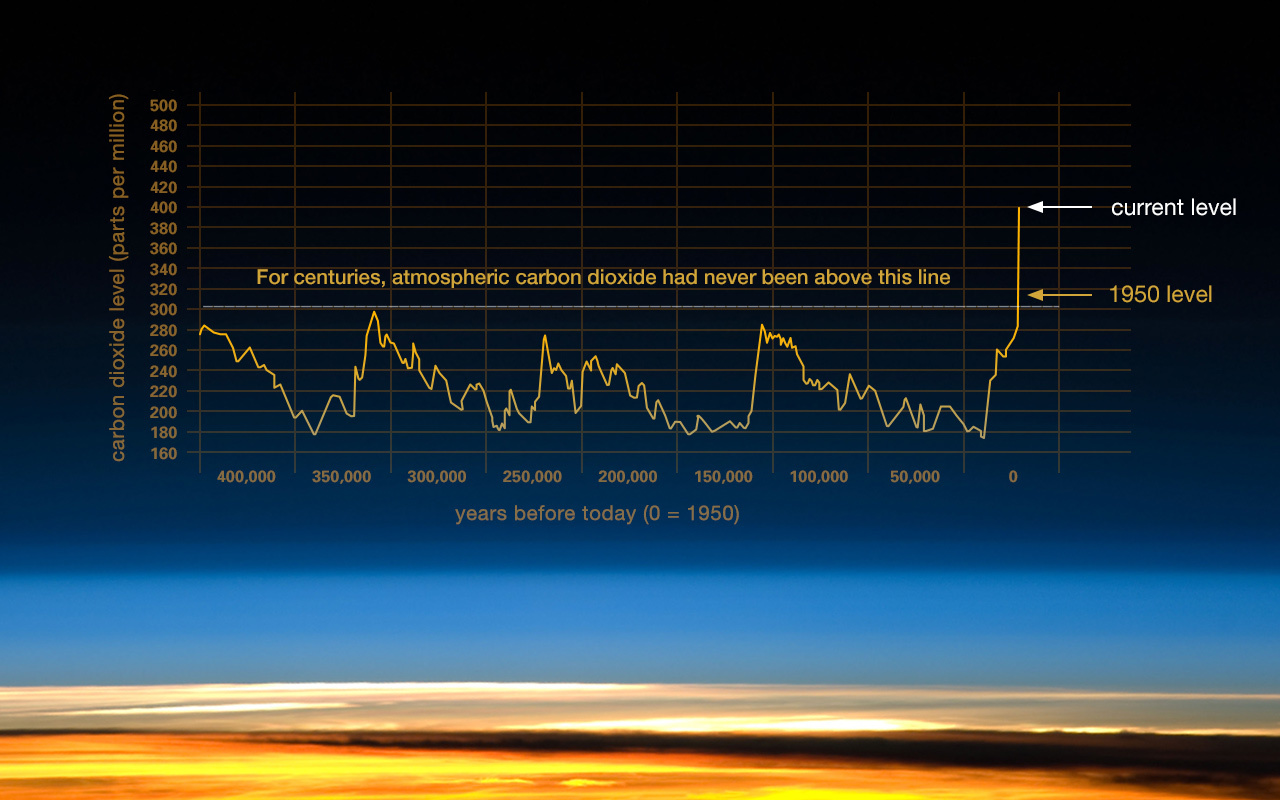
\includegraphics[width = .891\textwidth]{figure/1_1_1_nasa_co2.jpeg}
\caption{The evidence that atmospheric CO2 has increased since the Industrial Revolution began. Image courtesy: https://climate.nasa.gov/evidence}
\label{1_1_1_nasa_co2}
\end{figure}

\subsubsection{Conflicts and Wars}
An unbalanced energy distribution causes conflicts and wars. The wars, like Gulf War, are more or less derived from energy issues since WW2.\\

\subsubsection{Power Interruption}
With the use of unreliable electrical grids, power interruption occurs especially when a natural disaster, such as typhoon, earthquake, and wildfire, happens. Smart grids is more reliable than traditional grids. It’s possible to be build a dynamic technology, like Secondary Frequency Control (SFC), that grid operators need. Self-healing is possible when the storms hit, or physical attack occurs. Therefore, consumers not encounter power interruptions.\\

\subsubsection{Equal Rights to Use Natural Power}
Everyone should have his/her right to use natural resources equally. However, in most countries, the fact is that a few large companies occupy the dominant position of public funds and gradually form a monopoly market. Entrepreneurs use their centralised power to restrict consumers’ right to disagree.\\

However, the technologies should start with the customers. It is connected with intelligent devices that always communicate with each other. The system creates and stores energy throughout the day and any extra energy flows back onto the grid to power neighbours and businesses. Those smart energy buildings then power entire communities. It’s distributed, clean, and more cost-effective.\\

\subsubsection{New Issues from Clean Energy}
Using clean energy from renewable resource could be one of the ways to solve the problems above! In fact, recently, California Assembly passed a bill requiring 100 percent of the state’s electricity to come from carbon-free sources by the end of 2045. In China and Germany, renewables are outgrowing their grids. The public is accepting the idea of using electric cars instead of fuel cars.\\

However, these renewable energy sources interfaced with national or state power systems introduce new issues on stability, resilience, and reliability. Thus, power networks are under modification.\\

For countries like Switzerland, where 62\% of electricity comes from renewable sources, it’s another situation. Although it’s really friendly to the environment, energy instability has also increased. Sun doesn’t always shine, wind doesn’t always blow, and water doesn’t always flow.\\

\subsection{Solution: Secondary Frequency Control}
As these highly variable sources come to represent a growing portion of the grid, it becomes more and more important to develop an accurate and validated model to represent these units in the computational tools used to analyse the ancillary services of smart grids.\\

Smart grids power the modern city, and Secondary Frequency Control is one of the most important parts in smart grids to ensure the energy security in electricity systems and to allow increasing renewable energy penetration\\

Secondary Frequency Control ensures that the frequency of the electricity network is always restored to its nominal value when disturbances occur in the system. The frequency is one of the key “health” indicators of smart grids. Actively monitoring and controlling it ensure system security. This is done by remotely controlling the power output of generating units (both conventional and renewables) through a communication network.\\
\section{Thesis Outline} %1.2
This project consists of two parts: PART I Algorithms and PART II Test Case Scenario (Nordic).\\

PART I focuses on the task of understanding and building Secondary Frequency Control (SFC) model and PI control algorithm so that we are able to test our cases in PART II.\\


In Chapter~\ref{Chapter2}, we give an overview of Frequency Control, including Primary Frequency Control (PFC), Secondary Frequency Control (SFC) and Tertiary Frequency Control (TFC).\\

In Chapter~\ref{Chapter3}, we formally focus on the physical theory behind Secondary Frequency Control (SFC) which is the base of the whole project. We briefly discuss PID control and argue that we should use PI control to reduce the probability of risk. We then discuss how to build a communication layer on top of an existing smart grid simulator and how to design a centralised controller for stabilising the system. We describe the algorithms we built, the tuning methodology, and some implementations. We finally define the acceptable results based on the official report from Nordic, and with that, we build our own analytical tools. With these tools, we can plot a 2D and even a 3D diagram, find the eligible results and give feedback to our controller in PART II.\\

PART II views testing in a specific test case scenario (Nordic) as an important part such as the impact of different time delays. Detailedly,\\

In Chapter~\ref{Chapter4}, we focus on testing the system in a low time delay. We discuss how to choose an appropriate generator as a breaker and how to tune the range of  gain. Before simulating, we predict some expected results based on the physical theory behind Secondary Frequency Control (SFC). Then we present a comprehensive evaluation on the simulation results. We describe the results and compare them with the expected one. We discuss why my prediction had deviation or missing. We finally show a 2d plot and a simulation result.\\

In Chapter~\ref{Chapter5}, we discuss the impact of different time delays. We increase the delay and use the range of kp and ki in Chapter~\ref{Chapter4}. We explain why we think it is reasonable to continue using the range of gain in Chapter~\ref{Chapter4}. Then we predict the simulation results based on both the physical theory behind Secondary Frequency Control (SFC) and the results in Chapter~\ref{Chapter4}. Then we present a comprehensive evaluation on the complicated simulation results. We describe the results with a plotted 3d graph. We discuss some unpredictable results and some seemingly irregular data. We discuss the risk of the generators, like what we do in Chapter~\ref{Chapter4}, and how to remove unacceptable results. We  finally show a 3d plot and a best simulation result.\\

In Chapter~\ref{Chapter6}, we test Emergency Control and discuss the impact of different time delays without tuning gains. We firstly define Emergency Control although we have discussed it in Chapter~\ref{Chapter2}. We predict some results based on Secondary Frequency Control (SFC) and the conclusions in Chapter~\ref{Chapter4}. After implementing and analysing the results, we discuss why my predictions are “wrong”. We finally do a risk assessment for the system as we did before.\\


We finally conclude in Chapter~\ref{Chapter7}.\\
\section{Contributions} %1.3
The contributions of this thesis are summarised as follows:\\
\begin{itemize}
  \item I built a communication layer on top of an existing Smart Grid simulator and design a centralised controller for stabilising the system.\\
  
  \item I researched situations that cause disturbances, including generators interruption, high time delays and blackout. I built a series of efficient models for analysing the performance of the system and remove any unacceptable results. After hundreds of manual data proofreading, these models has demonstrated superior analytical ability.\\
  
  \item I built an optimal controller for stabilising the frequency based on the centralised controller and the analytical models above. This optimal controller has demonstrated superior performance of restoring frequency when disturbances occur in the system.\\
\end{itemize}


% PART I
\part{Algorithm}

\chapter{An Overview of Frequency Control}
\label{Chapter2}
% section:
Every country has its nominal frequency of the oscillations of alternating current in an electric power grid transmitted from a power station to the end-user. For instance, the nominal value is 50Hz \cite{papadopoulos2009distribution} in the UK while it’s 60Hz \cite{komarnicki2008practical} in USA.\\

However, \cite{machowski2011power} if a load is suddenly connected or disconnected to the system, or if the protection equipment suddenly disconnects a generating, there be a distortion in the power balance between that delivered by the turbines and that consumed by the loads. This imbalance is initially covered from \cite{machowski2011power} the kinetic energy of rotating rotors of turbines, generators and motors and, as a result, the frequency in the system change.

If there is a mismatch between the generation and the demand, for instance, due to the outage of one generating unit, then the frequency starts to drop down.  

If no control is applied, the frequency will largely deviates and then reaches a meagre and steady-state value, due to which the electrical grid is shut down.\\

\begin{figure}[t]
\center
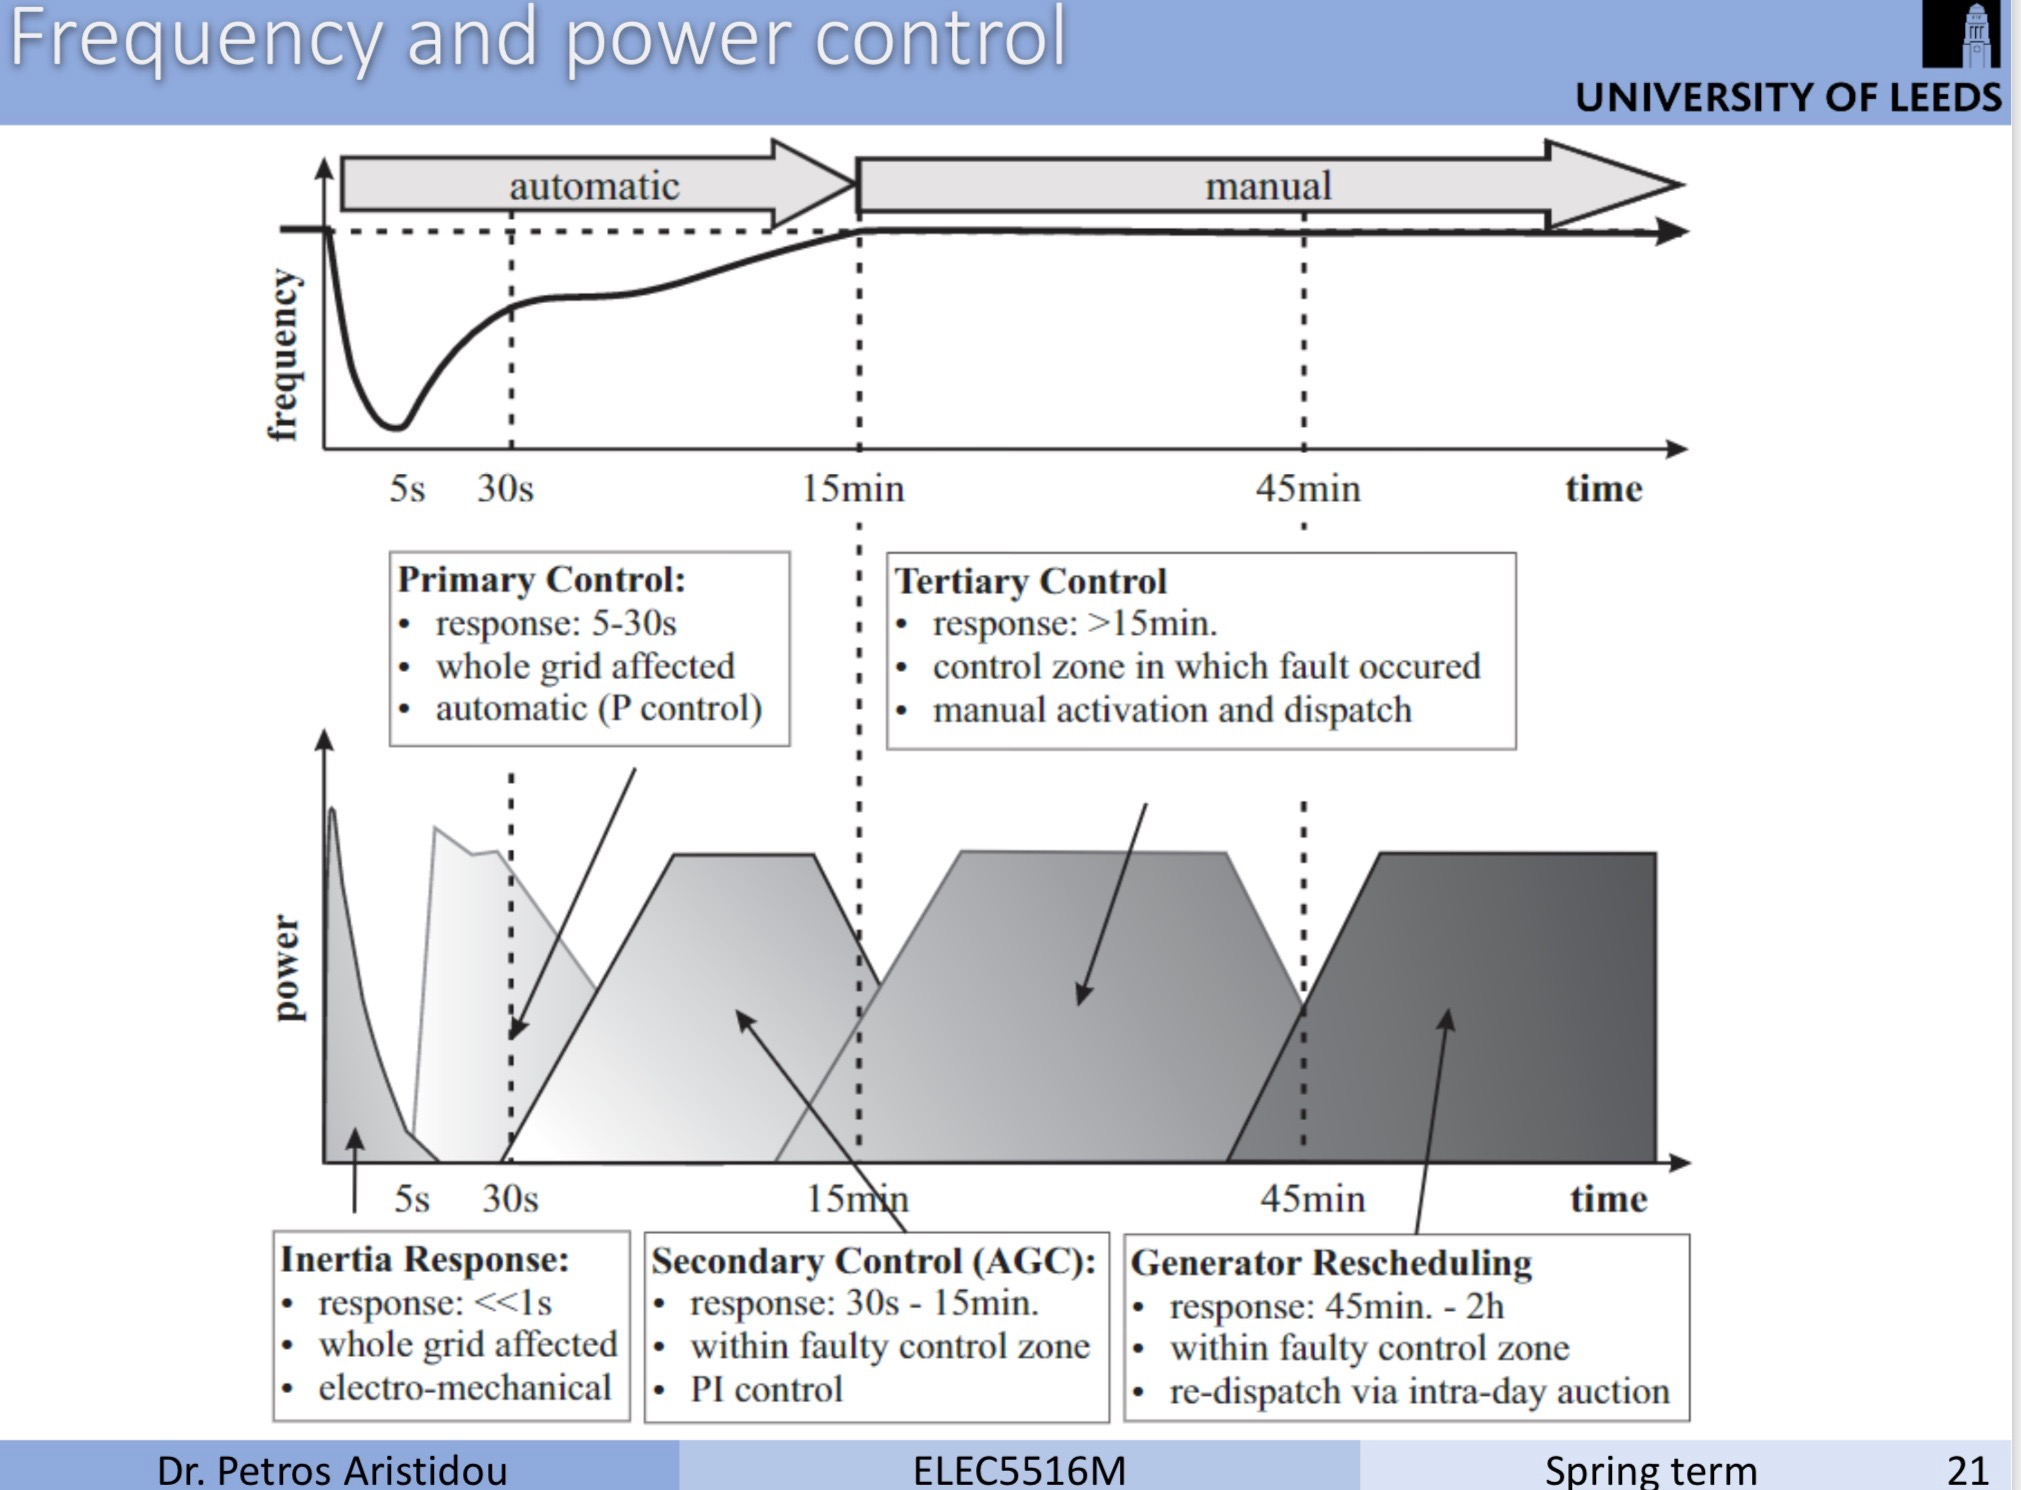
\includegraphics[scale=0.2]{figure/2_1_freq.jpeg}
\caption{Frequency and power control.}
\label{2_1_freq}
\end{figure}

The mechanism of primary frequency control is to restore the active power balance in a power system. After primary control takes place, the power balance is restored at a lower or higher frequency. Normally it takes seconds and responses from 5 seconds to 30 seconds. It is a partly Automatic Generation Control.\\


However, the frequency does not go back to its nominal value and remains at a steady-state value below or above the nominal one. To avoid damages to equipment and loads, we need secondary frequency control to \cite{machowski2011power} restore the frequency balance to its nominal value or to eliminate the steady-state error/frequency error. Normally it takes minutes and responses from 30 seconds to 15 minutes. It is a fully Automatic Generation Control.\\


Tertiary Frequency Control encompasses actions taken to capture current and future emergencies by getting resources. Alternate deployment and recovery after a disturbance are common types of Tertiary Control. Normally it takes dozens of minutes and responses longer than 15 minutes. It is a fully manual control.

\chapter{PID Control Algorithm}
\label{Chapter3}
% section:
\section{The physical theory behind Secondary Frequency Control} %3.1

From Chapter~\ref{Chapter2}, we mentioned that disturbances occur in the system, there be a distortion in the power balance between that delivered by the turbines and that consumed by the loads. The imbalance is from the kinetic energy of rotating rotors of turbines, generators and motors and, thus, the frequency in the system change. If no control is applied, the frequency largely deviates and then reaches a meagre and steady-state value, due to which the electrical grid is shut down.  

We also mentioned that the system will start Primary Frequency Control firstly and then the frequency will remain at a steady-state value below or above the nominal one. After that, Secondary Frequency Control starts. 

The mechanism of Secondary Frequency Control is to restore the frequency to the nominal one. 

Secondary frequency control, or load frequency control (LFC), or automatic generation control (AGC), is an automatic control that restores the frequency back to its nominal value in a centralised way. It's implemented that is activated after the primary frequency control. Typically, it takes 30 seconds to 15 minutes. 

\begin{figure*}[htbp]
\centering
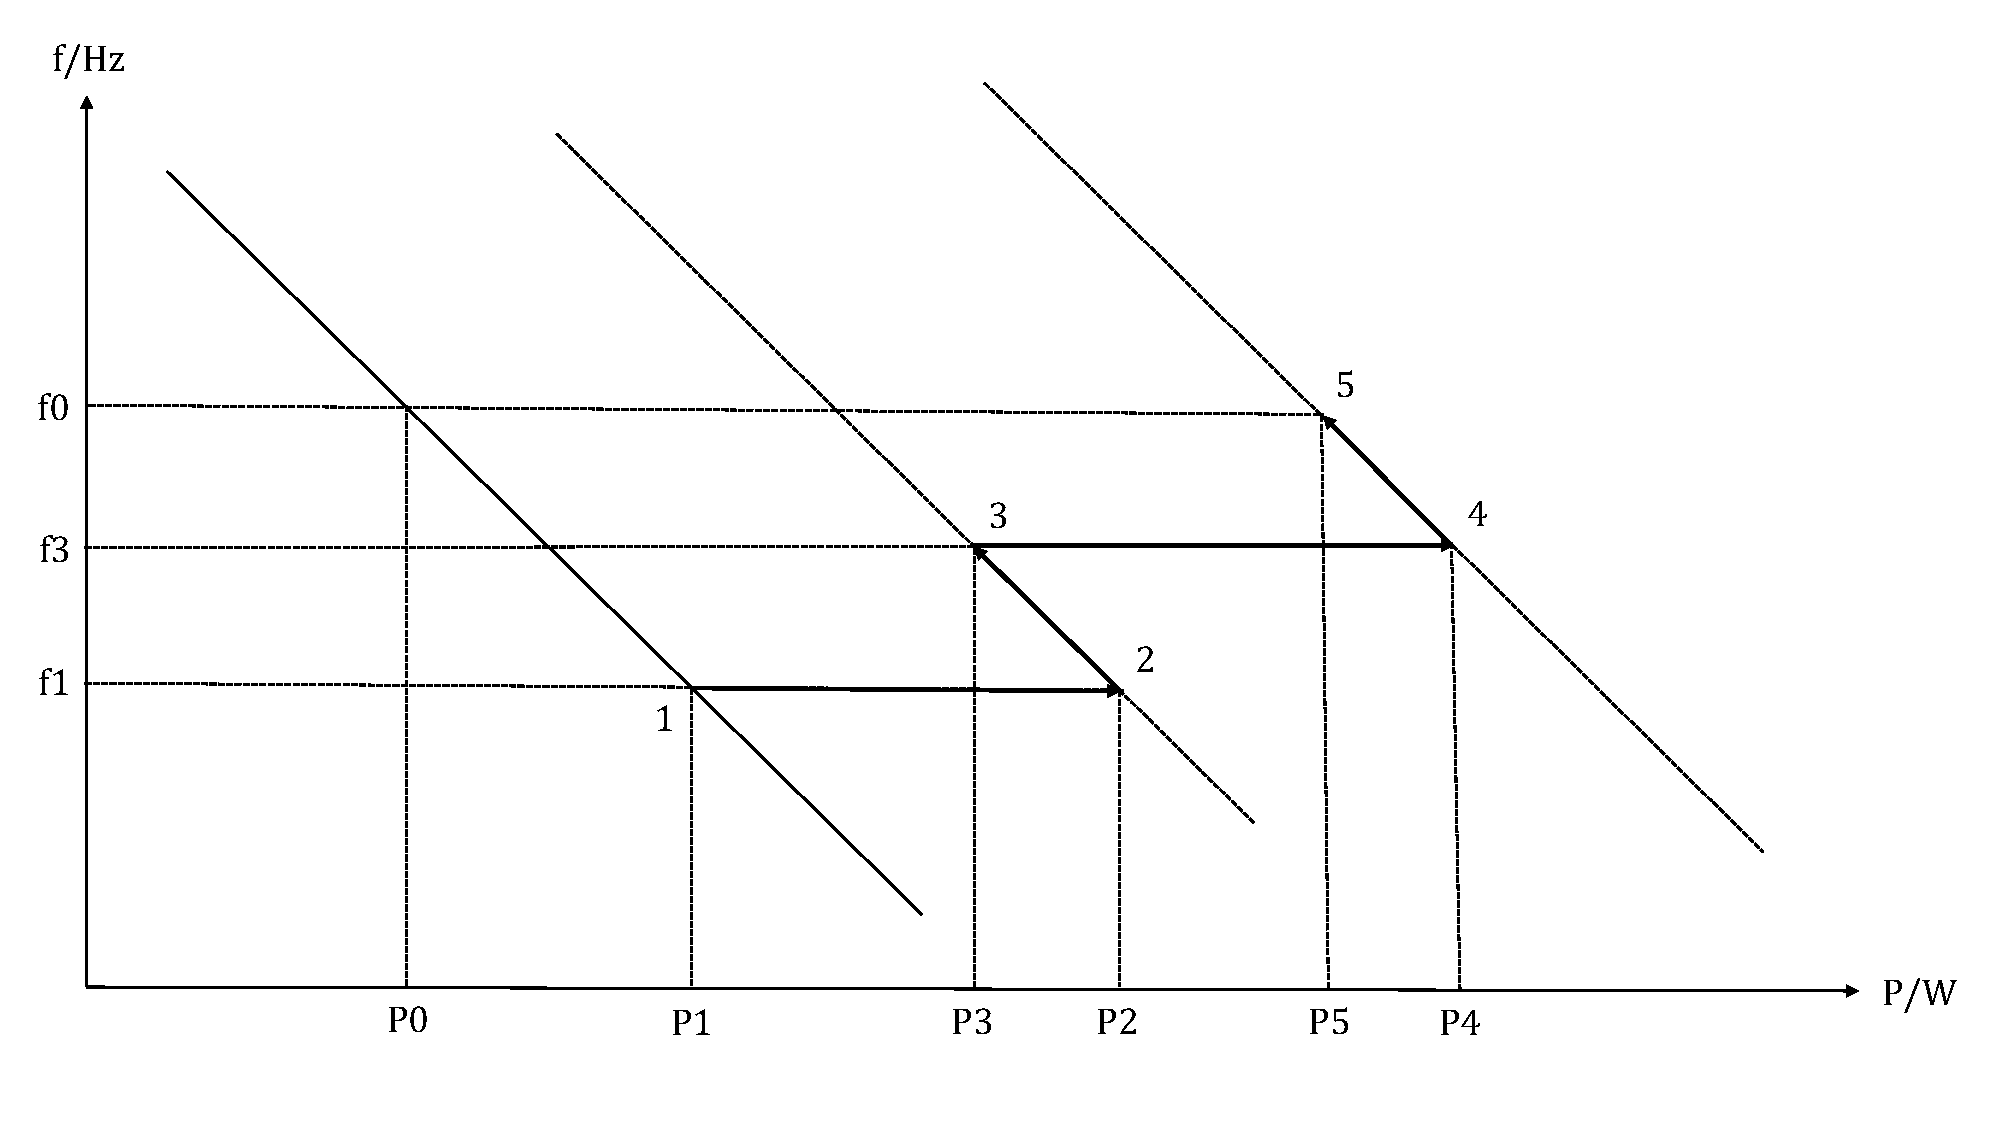
\includegraphics[width = 0.816\textwidth]{figure/3_1_Equilibrium.pdf}
\caption{Equilibrium points for an increase in the power demand.}
\label{3_1_Equilibrium}
\end{figure*}

According to Figure~\ref{3_1_Equilibrium}, frequency value rise when reference power rises. Assumed point 1 is the situation after primary frequency control happens and point 5 has the nominal value of frequency. When trying to raise the reference power a little bit, point 1 shift to point 2. Due to the power rise, the frequency of the system rise, so point 2 move to point 3. Changing more reference power of individual governors move the overall generation characteristic of the system upwards. Eventually, this lead to the restoration of the rated frequency ($f0$). 

\begin{figure}[htb]
\centering
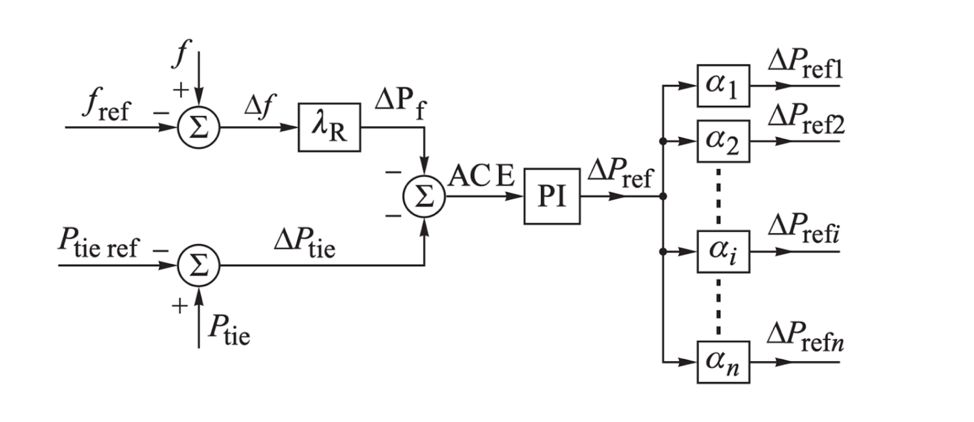
\includegraphics[width = 0.891\textwidth]{figure/3_1_Functional.png}
\caption{Functional diagram of a central regulator.}
\label{3_1_Functional}
\end{figure}

As seen in Figure~\ref{3_1_Functional}, the frequency ($f$) be measured in the local network and compared with the reference frequency to produce an amplified signal ($\Delta P_f$) that is proportional to the frequency deviation ($\Delta f$). For instance, if the frequency is smaller the reference frequency, then the signal $\Delta P_f$ be negative. Thus, input signal ACE is positive according to the functional diagram. Therefore, output signal $\Delta P_f$ is positive and it adjust the system by raising the reference value of the power. Then the system have a new frequency value ($f_{n e w}$) that go through the functional diagram again to compare the difference with the value of the reference frequency. ACE won’t be zero and the frequency won’t be stopped adding until we remove any error. 

In this standard case, which ignores the existence of tie-line interchange error, the only condition to remove errors is the frequency deviation ($\Delta f$) equals to zero. 

\begin{figure}[htbp]
\centering
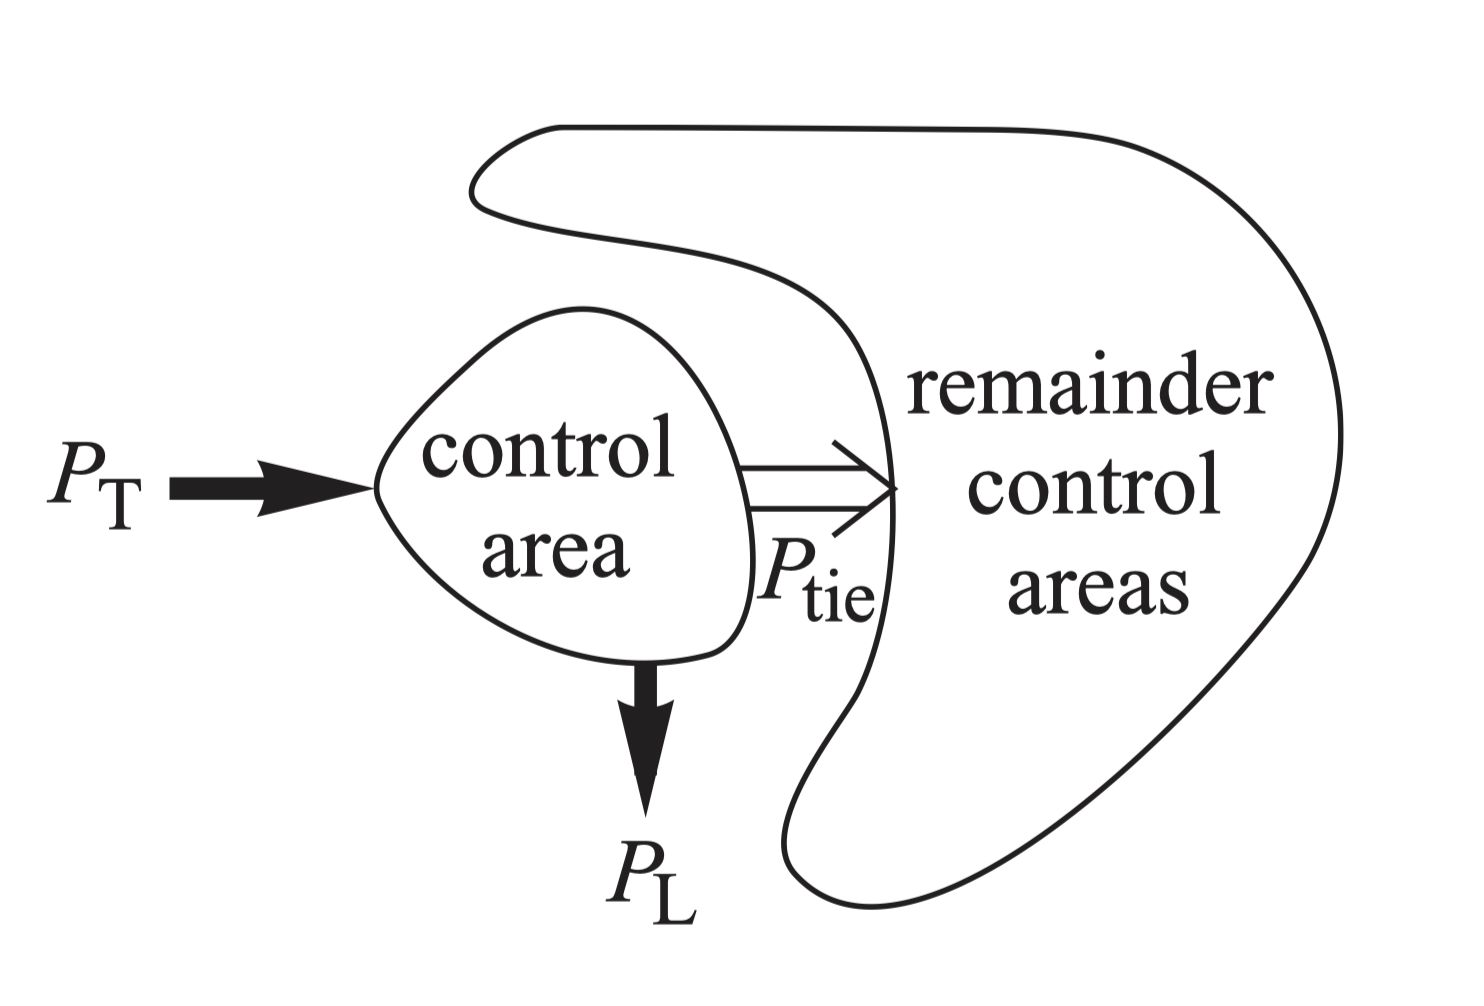
\includegraphics[width =0.819\textwidth]{figure/3_1_Power.png}
\caption{Power balance of a control area.}
\label{3_1_Power}
\end{figure}

However, it would be more difficult if consider the situation of tie-line interchange error. In interconnected power systems, AGC is implemented in a way where each subsystem has its own regulator. As shown in Figure~\ref{3_1_Power}, the power system is in equilibrium if the total power generation ($P_T$), the total power demand ($P_L$) and the net tie-line interchange power ($P_{t i e}$) satisfy the condition in each subsystem: 

\begin{equation} \label{eq1}
P_T - (P_L + P_{t i e}) = 0
\end{equation}

The objective of each regulator of the subsystem is to maintain frequency at the nominal level and to maintain net tie-line interchanges from the given area at the scheduled values. If there is a disturbance in one subsystem, then regulators in each subsystem should try to restore the frequency and net tie-line interchanges. Each subsystem regulator should enforce an increased generation covering its own area power imbalance and maintain planned net tie-line interchanges.

As shown in Figure~\ref{3_1_Functional}, to obtain a signal proportional to the tie-line interchange error $(\Delta P_{tie})$, the information on power flows in the tie-lines is sent via telecommunication lines to the central regulator which compares it with the reference value. Then the signal $(\Delta P_f)$ is added to the net tie-line interchange error $(\Delta P_{tie})$ so that ACE is


\begin{equation} \label{eq2}
ACE = - \Delta P_f - \Delta P_{tie}
\end{equation}


The situation here is similar to the situation above, where we ignore tie-line interchange error, except for the condition to remove errors. In this book, it shows us zeroing of errors can be achieved in two ways: zeroing of both errors ($ P_{tie} = 0 $ and $ f = 0 $) and achieving a compromise between the errors ($\Delta P_f + P_{tie} = 0$ or $P_f = - \Delta P_{tie}$). 
\section{PID Controller} %3.2
PID controller can be written in the following equation:

\begin{equation} \label{eq3}
u(t) = k_p e(t) + k_i \int_{0}^{t} e(\tau) d\tau + k_d \frac{d e}{d t}
\end{equation}

 where u is the control signal and e is the error. The nominal value is also called the reference value or the setpoint. The controller’s output is therefore summed by three terms: the P-term, the I-term, and the D-term. The P-term is proportional to the error and its amplification factor is $k_p$. The I-term is proportional to the integral of the error and its amplification factor is $k_i$. The D-term is proportional to the derivative of the error and its amplification factor is $k_d$. 
 
 The function of the P-term is trying to send a control signal proportional to the error. For example, there is a signal whose value is 90 and we hope it can approach to 100 using P-term only. The error now is (100 - 90 = 10). Assumed that $k_p$ equals to 0.5, then control signal becomes (10 x 0.5 = 5). The new signal becomes (90 + 5 = 95). If we continue to repeat this flow, we find the new signal turns to 97.5, 98.75 and 99.375. It seems like the new signal is approaching to our nominal value and it approach to the nominal value if we continue updating the signal. 
 

However, there are two situations that we cannot ignore. Firstly, steady-state error occurs if $k_p$ is not set well. For example, if $k_p$ equals to 2, the error be 20 and the new signal be 110, 90, 110, 90,… The signal can not be restored to the nominal one forever.  

The second situation is that, in reality, the signal is not perfect and it has its own errors. In the first example above, we choose 0.5 as our amplification factor ($k_p$) and thus the first new signal be 95. However, it is a possible the new signal will be lost its signal by 5 units every time after the control. Finally, the signal will remain 90 and the error will be 10.  

\begin{figure}[t]
\center
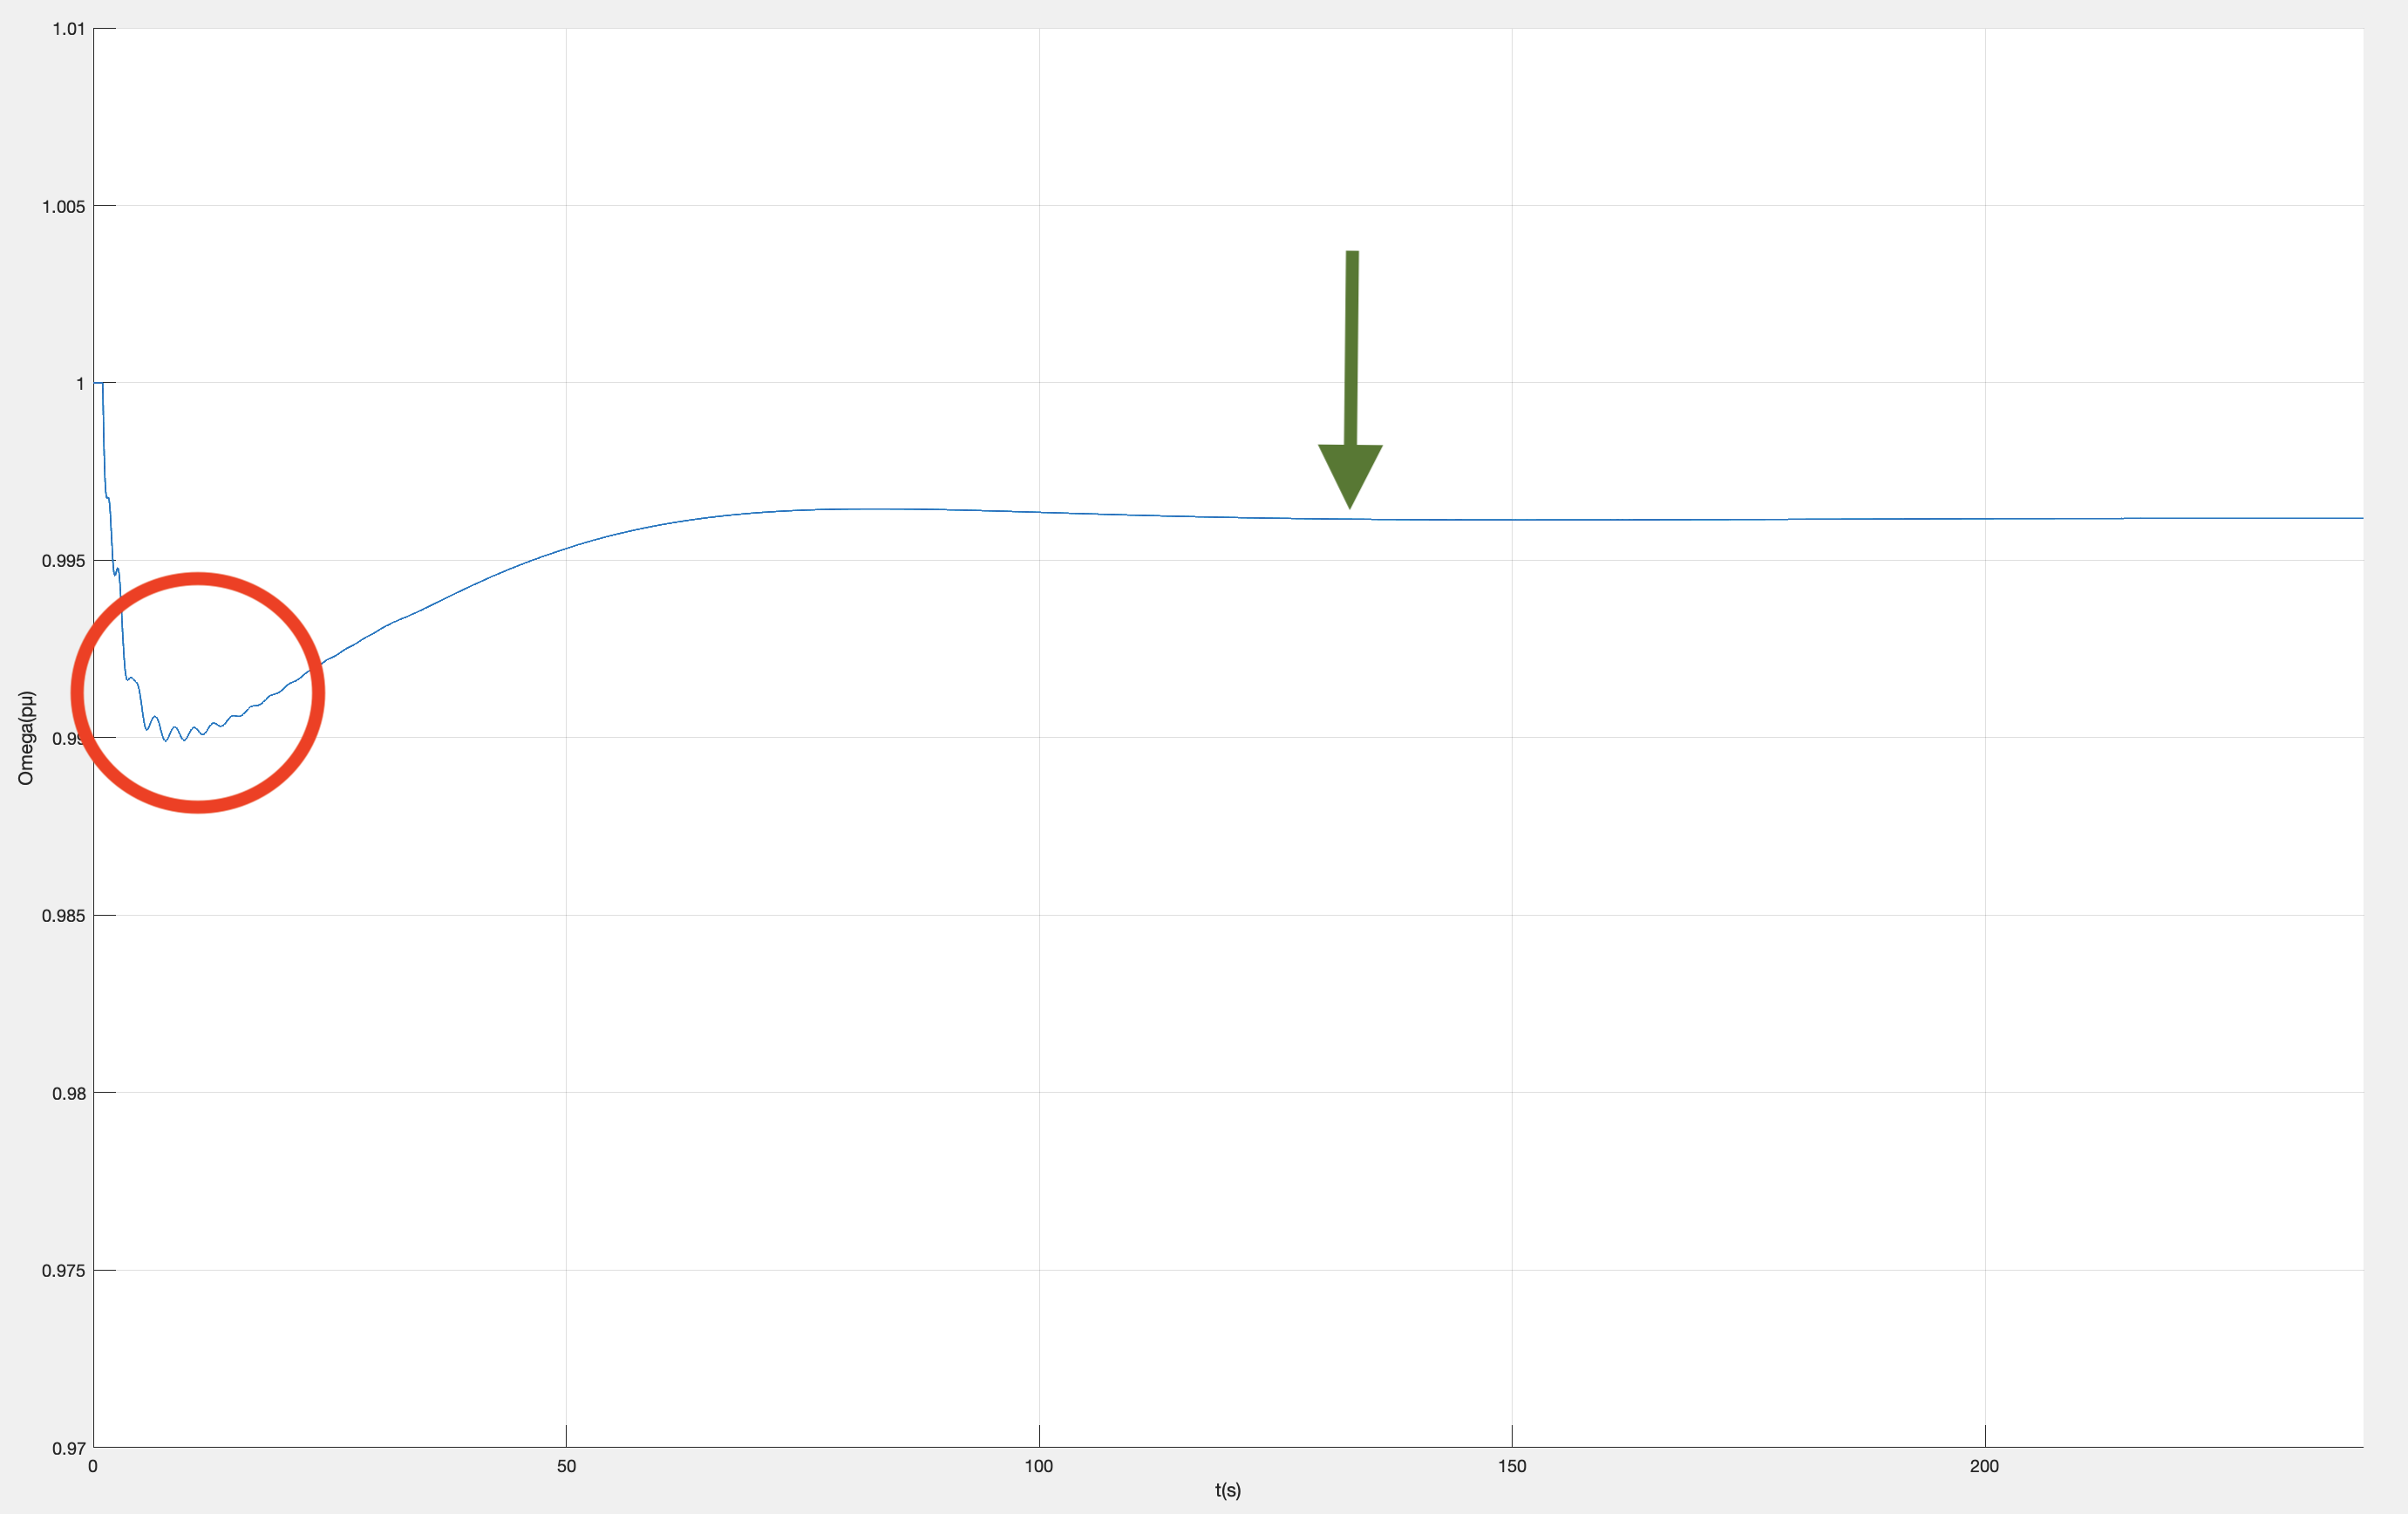
\includegraphics[scale=0.3]{figure/3_2_steady.png}
\caption{Steady-state error and high frequency component in a signal.}
\label{3_2_steady}
\end{figure}

In reality, whatever it is the automobile control system, the electronic compass control system or the Automatic Generation Control, the steady-state errors occurs if we use P control only. 

We introduce the I-term to remove such a steady-state error. Briefly, the integral of the error accumulate the previous errors and the I-term is proportional to the integral of the error, which means the I-term is proportional to previous accumulated errors. The integral of the error will not be zero, unless the error is removed. Gradually, the controlled signal will be larger and the new signal will approach to the nominal value. 

To the D-term, it is proportional to the derivative of the error. In another way, the D-term is proportional to the gradient of the signal. Thus, the D-term amplifies the high frequency component in the signal and will disturb the system. 
\section{PI Control Model} %3.3
At this point, we are equipped with all the building blocks. Let's first recap a PI control model. In PI control, we need to know the value of error and the value of integral of the error. Error is defined as the difference between the nominal value and the signal. In AGC, the nominal value is the nominal frequency in the country (50 Hz or 60 Hz) and the signal is the actual frequency sending into the controller. 

To the integral of the error, it should be realised that it is helpful to use discrete mathematics. In discrete mathematics, the value of integral of the error is the accumulated error. Thus, in Python, we can use time-step to help calculating the integral of the error.  Detailedly, in program, we can represent output as 

\begin{figure}[!htbp]
\center
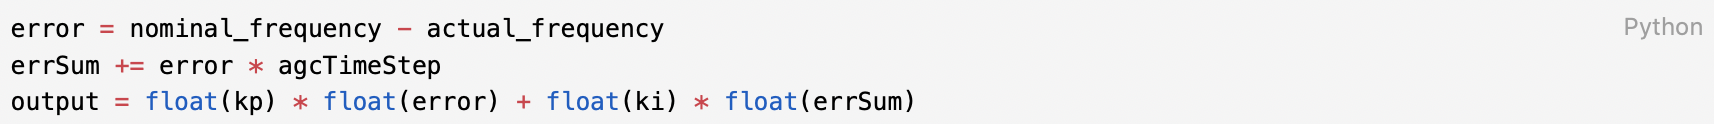
\includegraphics[scale=0.5]{figure/3_3_code1.png}
\caption{Python: PI control algorithm.}
\label{3_3_code1}
\end{figure}

where nominal frequency is 1.0 and we can directly get actual frequency from the simulation. 

Next, we should send output signal to generators through the command, 

\begin{figure}[!htbp]
\center
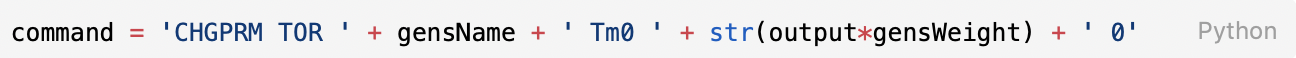
\includegraphics[scale=0.65]{figure/3_3_code2.png}
\caption{Python: send corrections to the generators.}
\label{3_3_code2}
\end{figure}

where, 'gensName' is the name of generator such as g1, g2 or g9. '1/gensWeight' is $\alpha$ in the Figure~\ref{3_1_Functional}. We use $\alpha$ to ask power proportional to these generators' nominal power.\\

Furthermore, we need to consider deadband control. The deadband refers to the range of input signal when output signal is zero in the domain of transfer signal. In our case, as shown in Figure~\ref{3_3_deadband}, it refers to the range of time when frequency does not change.  

\begin{figure}[!htbp]
\center
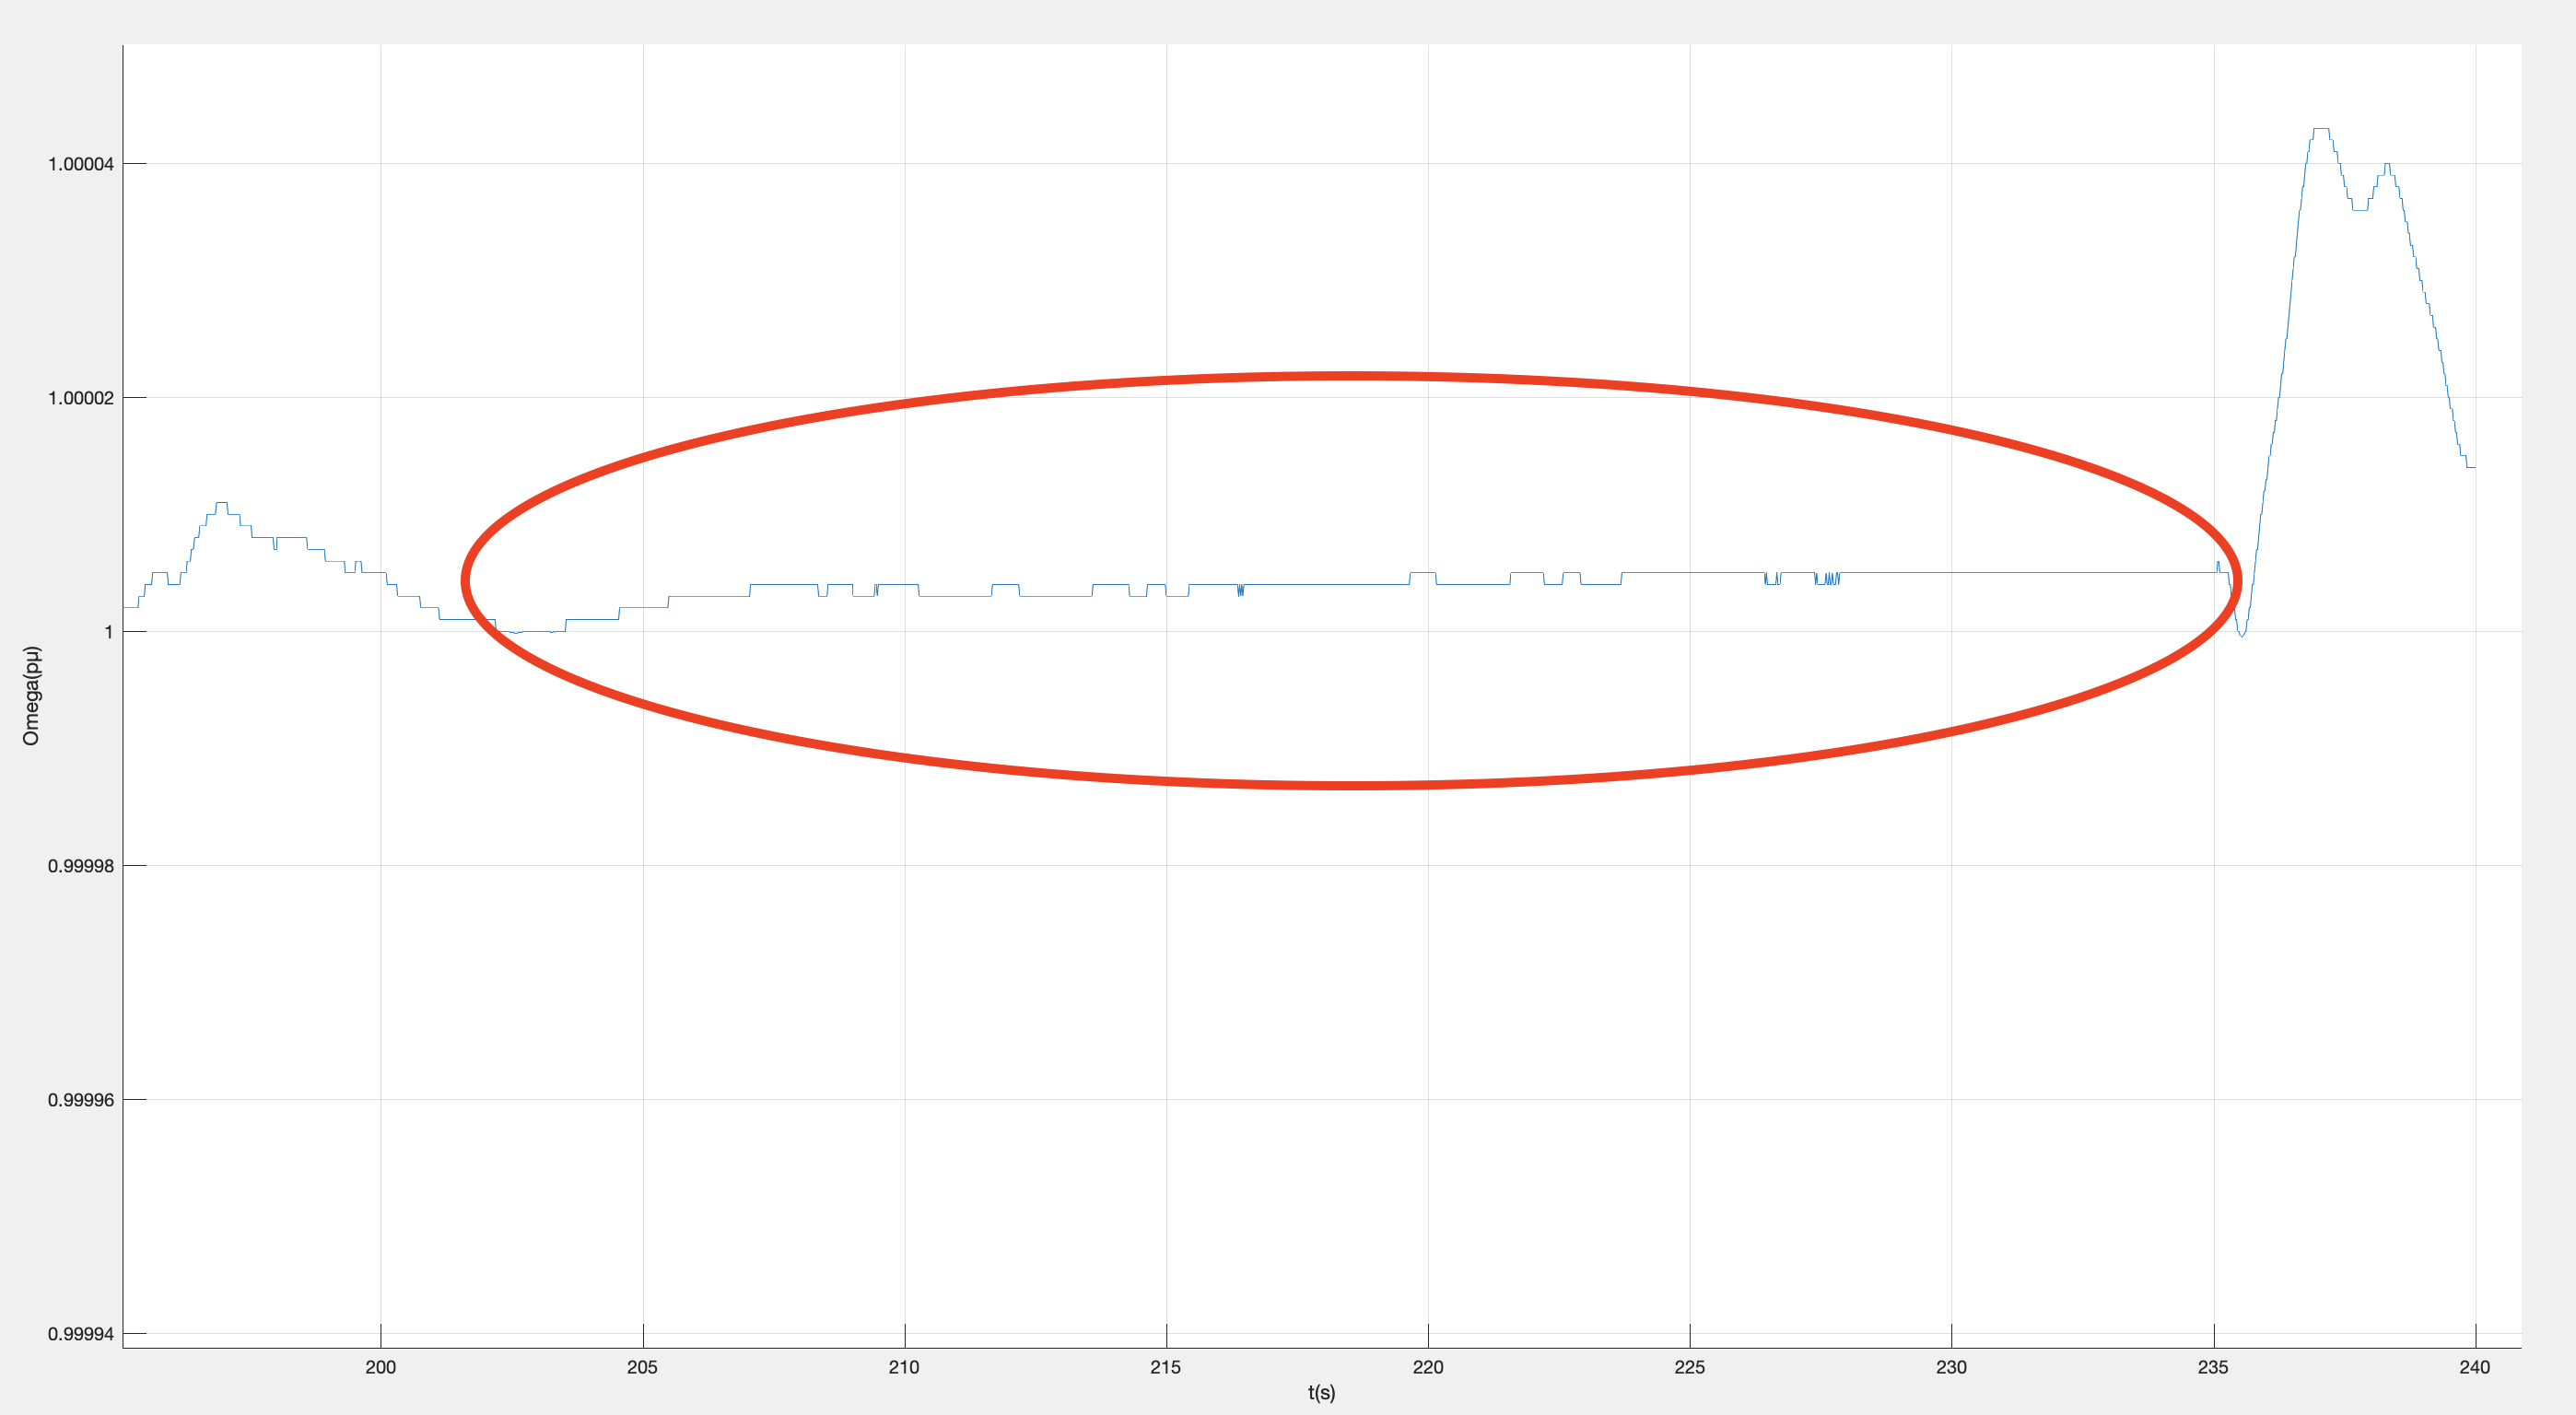
\includegraphics[scale=0.3]{figure/3_3_deadband.png}
\caption{Deadband in SFC.}
\label{3_3_deadband}
\end{figure}


However, in theory, it is impossible to remove deadband totally. The aim to use deadband control is: 
	
    (1). Make the frequency value as small as possible in the deadband area, so we can assume that tiny error is no error;
    
	(2). Make the deadband area as long as possible, so we can keep the frequency in the system stable in a relatively long time. 

Thus, we need to choose two parameters in our deadband control: acceptable frequency range in deadband area and control results. 

The acceptable frequency range is a suitable tiny frequency range that we allow deadband occurs.\\

For control results, we have three situations. One of them is without deadband control. Another situation is to make error be zero in the deadband area. The last situation is to make the error and the sum of error be zero at the same time.

\begin{figure}[htbp]
\center
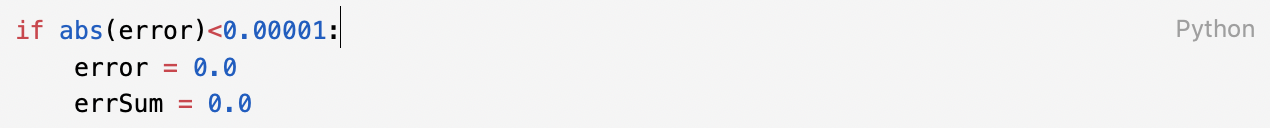
\includegraphics[scale=0.65]{figure/3_3_deadband_code.png}
\caption{Deadband controller.}
\label{3_3_deadband_code}
\end{figure}

Finally, as shown in the Figure~\ref{3_3_deadband_code}, we choose the frequency range in the deadband from -0.000001 Hz to 0.000001 Hz and we make the error and the sum of error be zero at the same time after the deadband control starts. Figure~\ref{3_3_deadband_result} shows the comparison between one without deadband control and one with deadband control. It shows that our deadband control is a more suitable solution for the system. 

\begin{figure}[!htbp]
\center
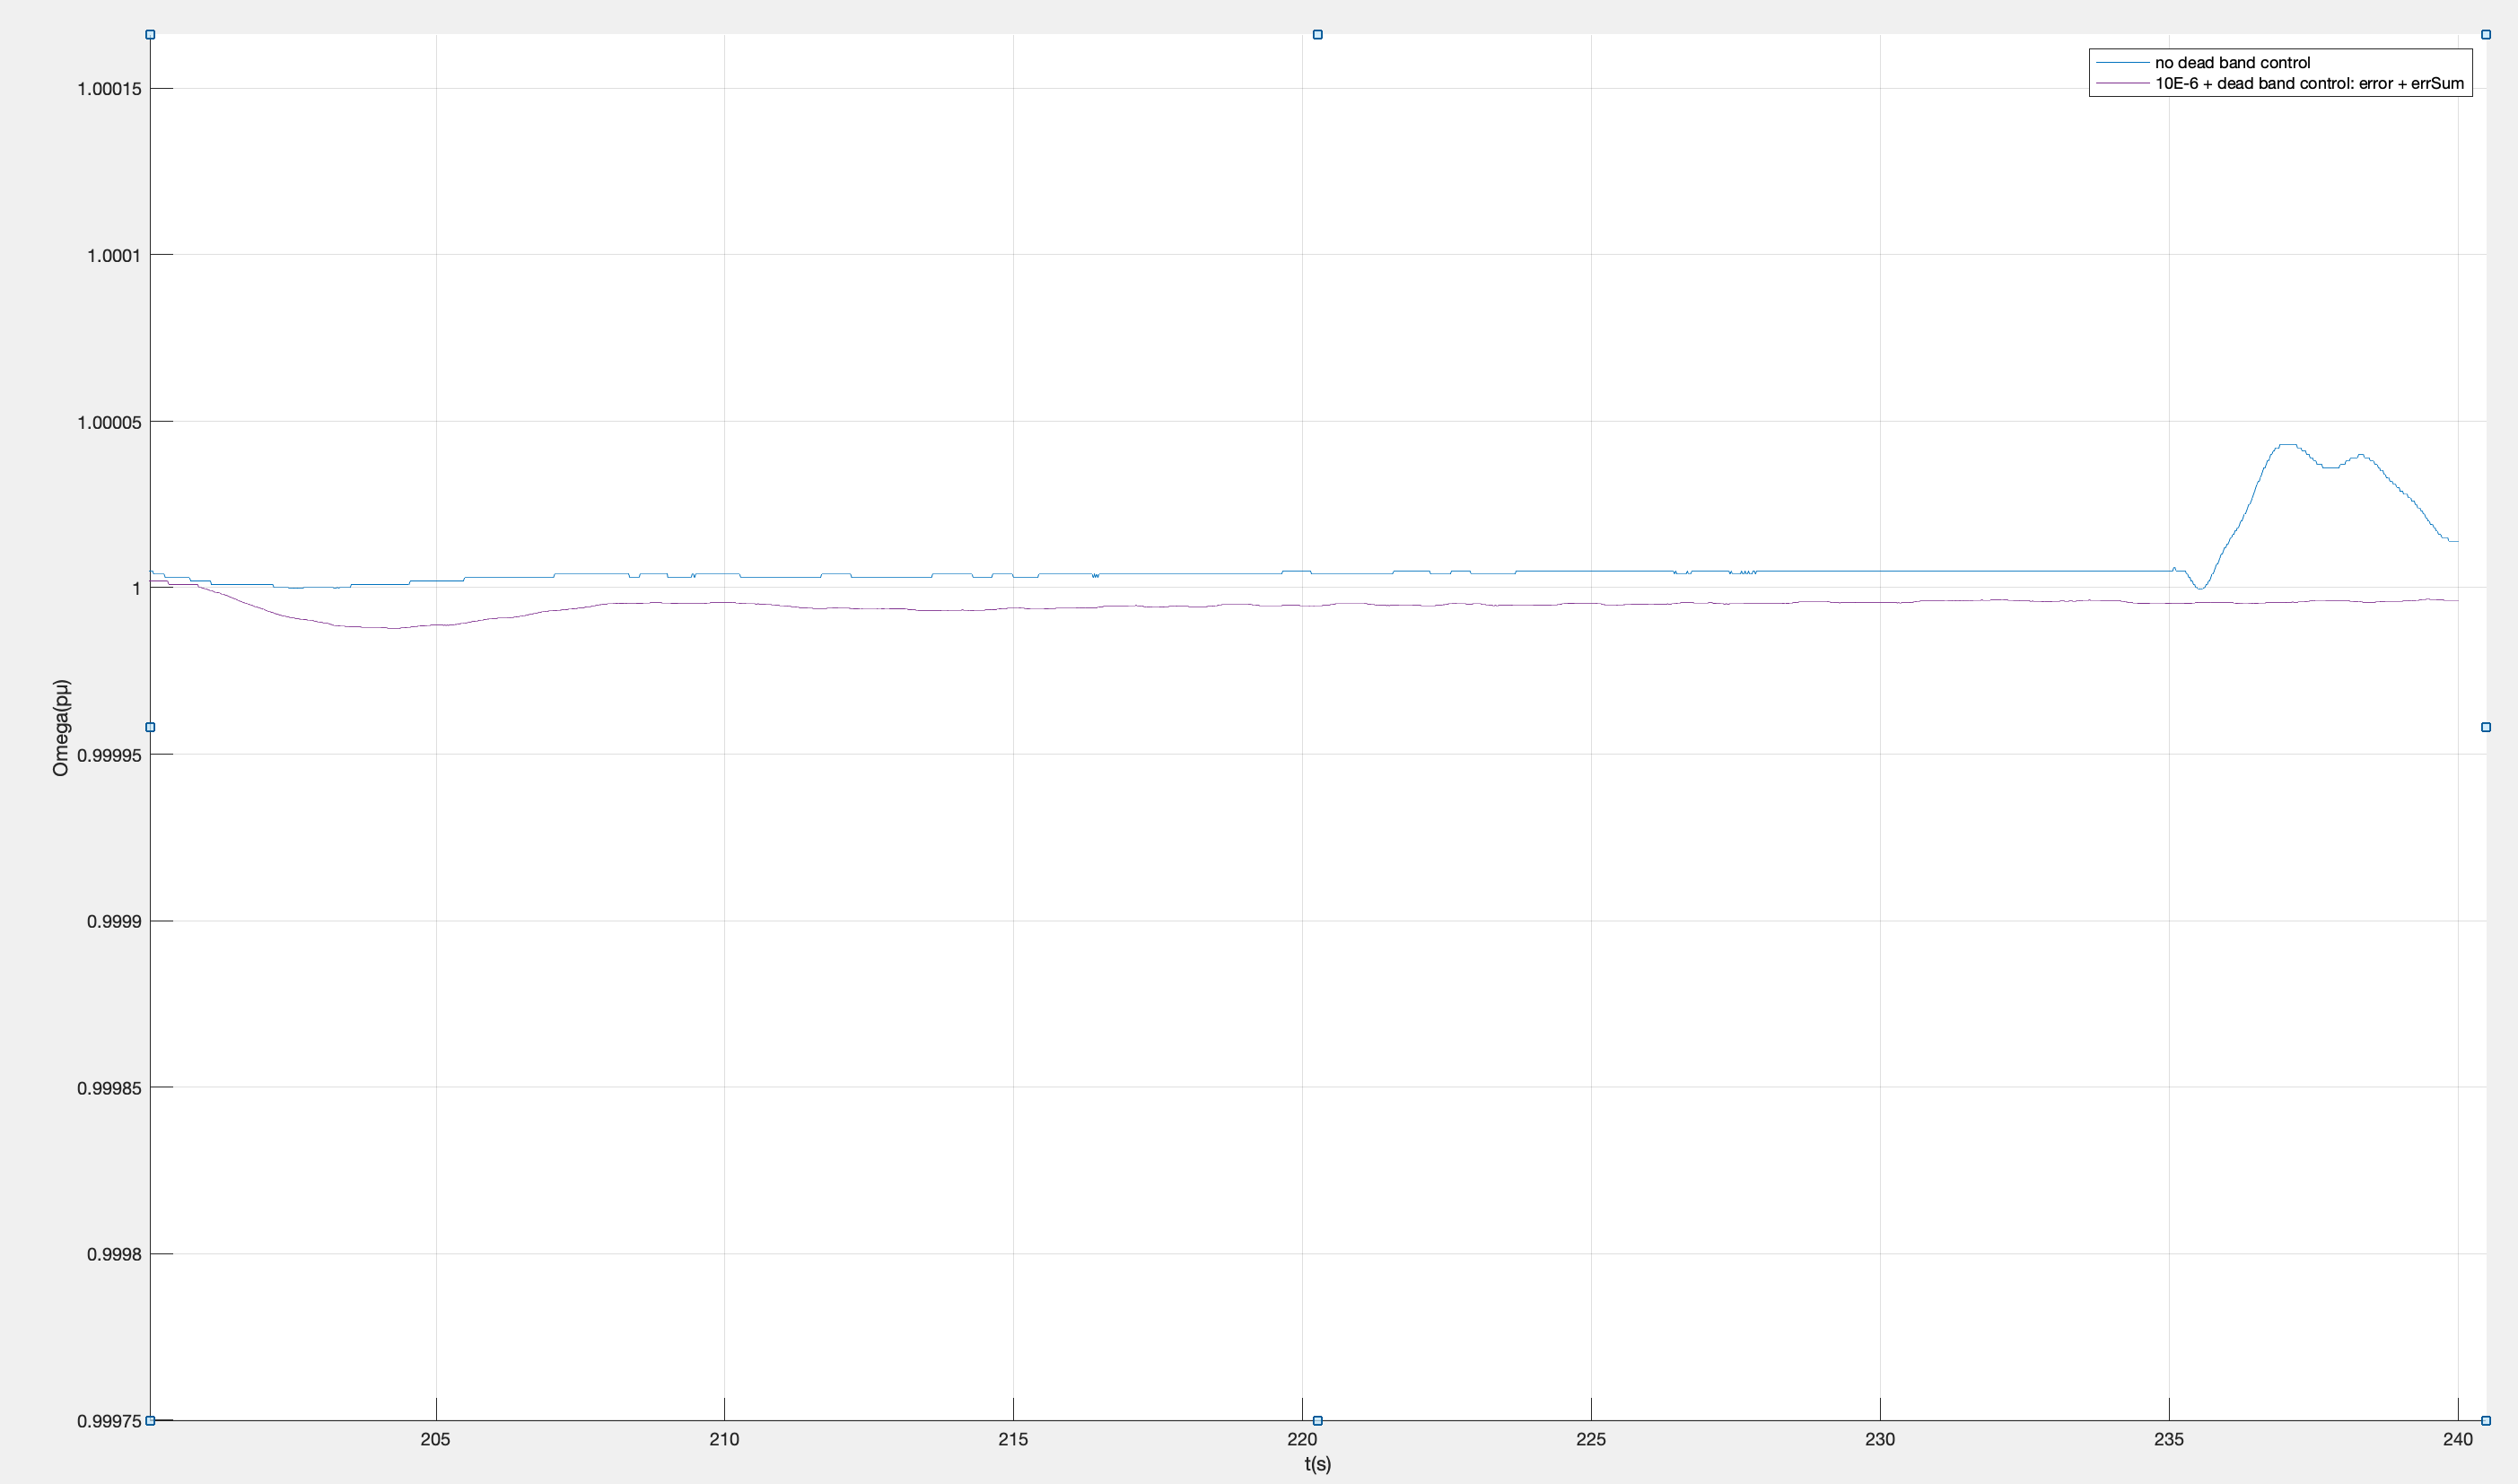
\includegraphics[scale=0.2]{figure/3_3_deadband_result.png}
\caption{Comparison: with and without deadband control.}
\label{3_3_deadband_result}
\end{figure}



We get the input from the existing smart grid simulator and send output to the existing smart grid simulator via our controller. Thus, a communication layer is formed.

Multiple hard-coded parameters, like the disconnected generator, the generators we asked for their power, amplification factor and time delay, are removed and added into main function so we can test our system comprehensively and easily. 
\section{Tuning Methodology } %3.4
\label{section3.4}
\subsection{Tuning Model} %3.4.1
Imagine if we have a 2D plane with the horizontal axis kp and the vertical axis ki, we can use the points on the plane to represent all the acceptable combination of kp and ki. 

\begin{figure}[!htbp]
\minipage{0.33\textwidth}
  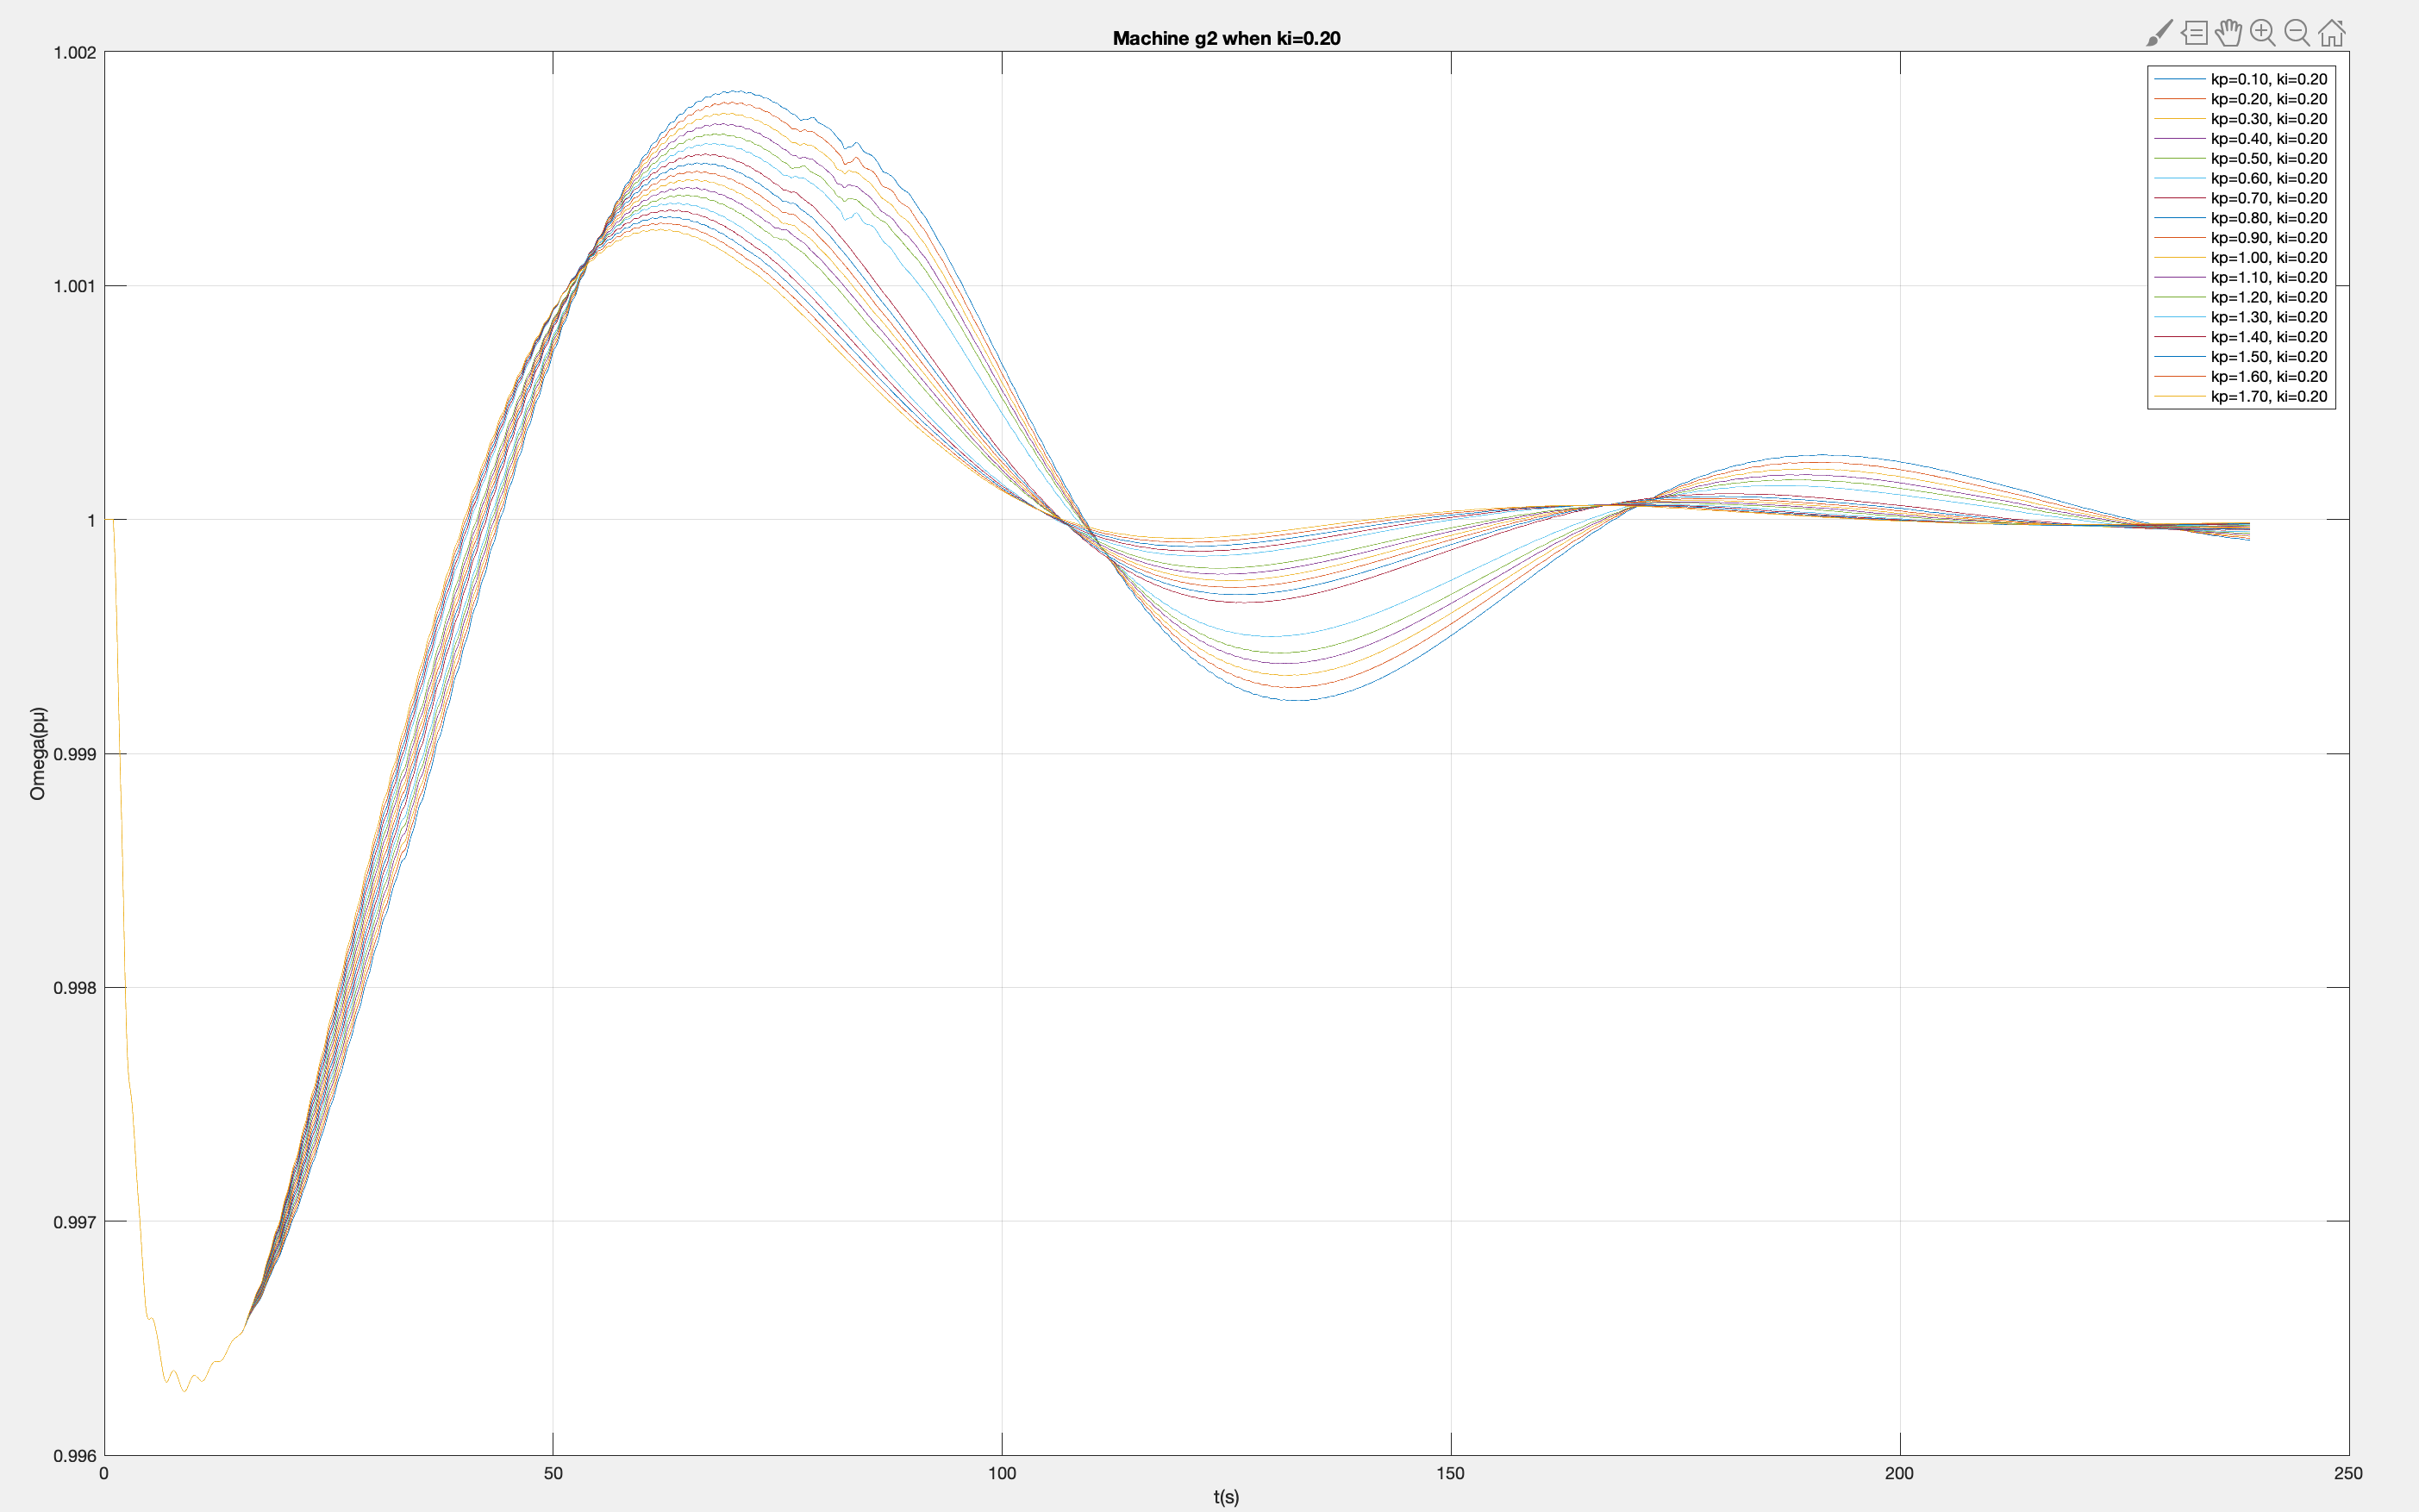
\includegraphics[width= \linewidth]{figure/3_4_1_tune_ki_1.png}
  %\caption{A really Awesome Image}\label{fig:awesome_image1}
\endminipage\hfill
\minipage{0.33\textwidth}
  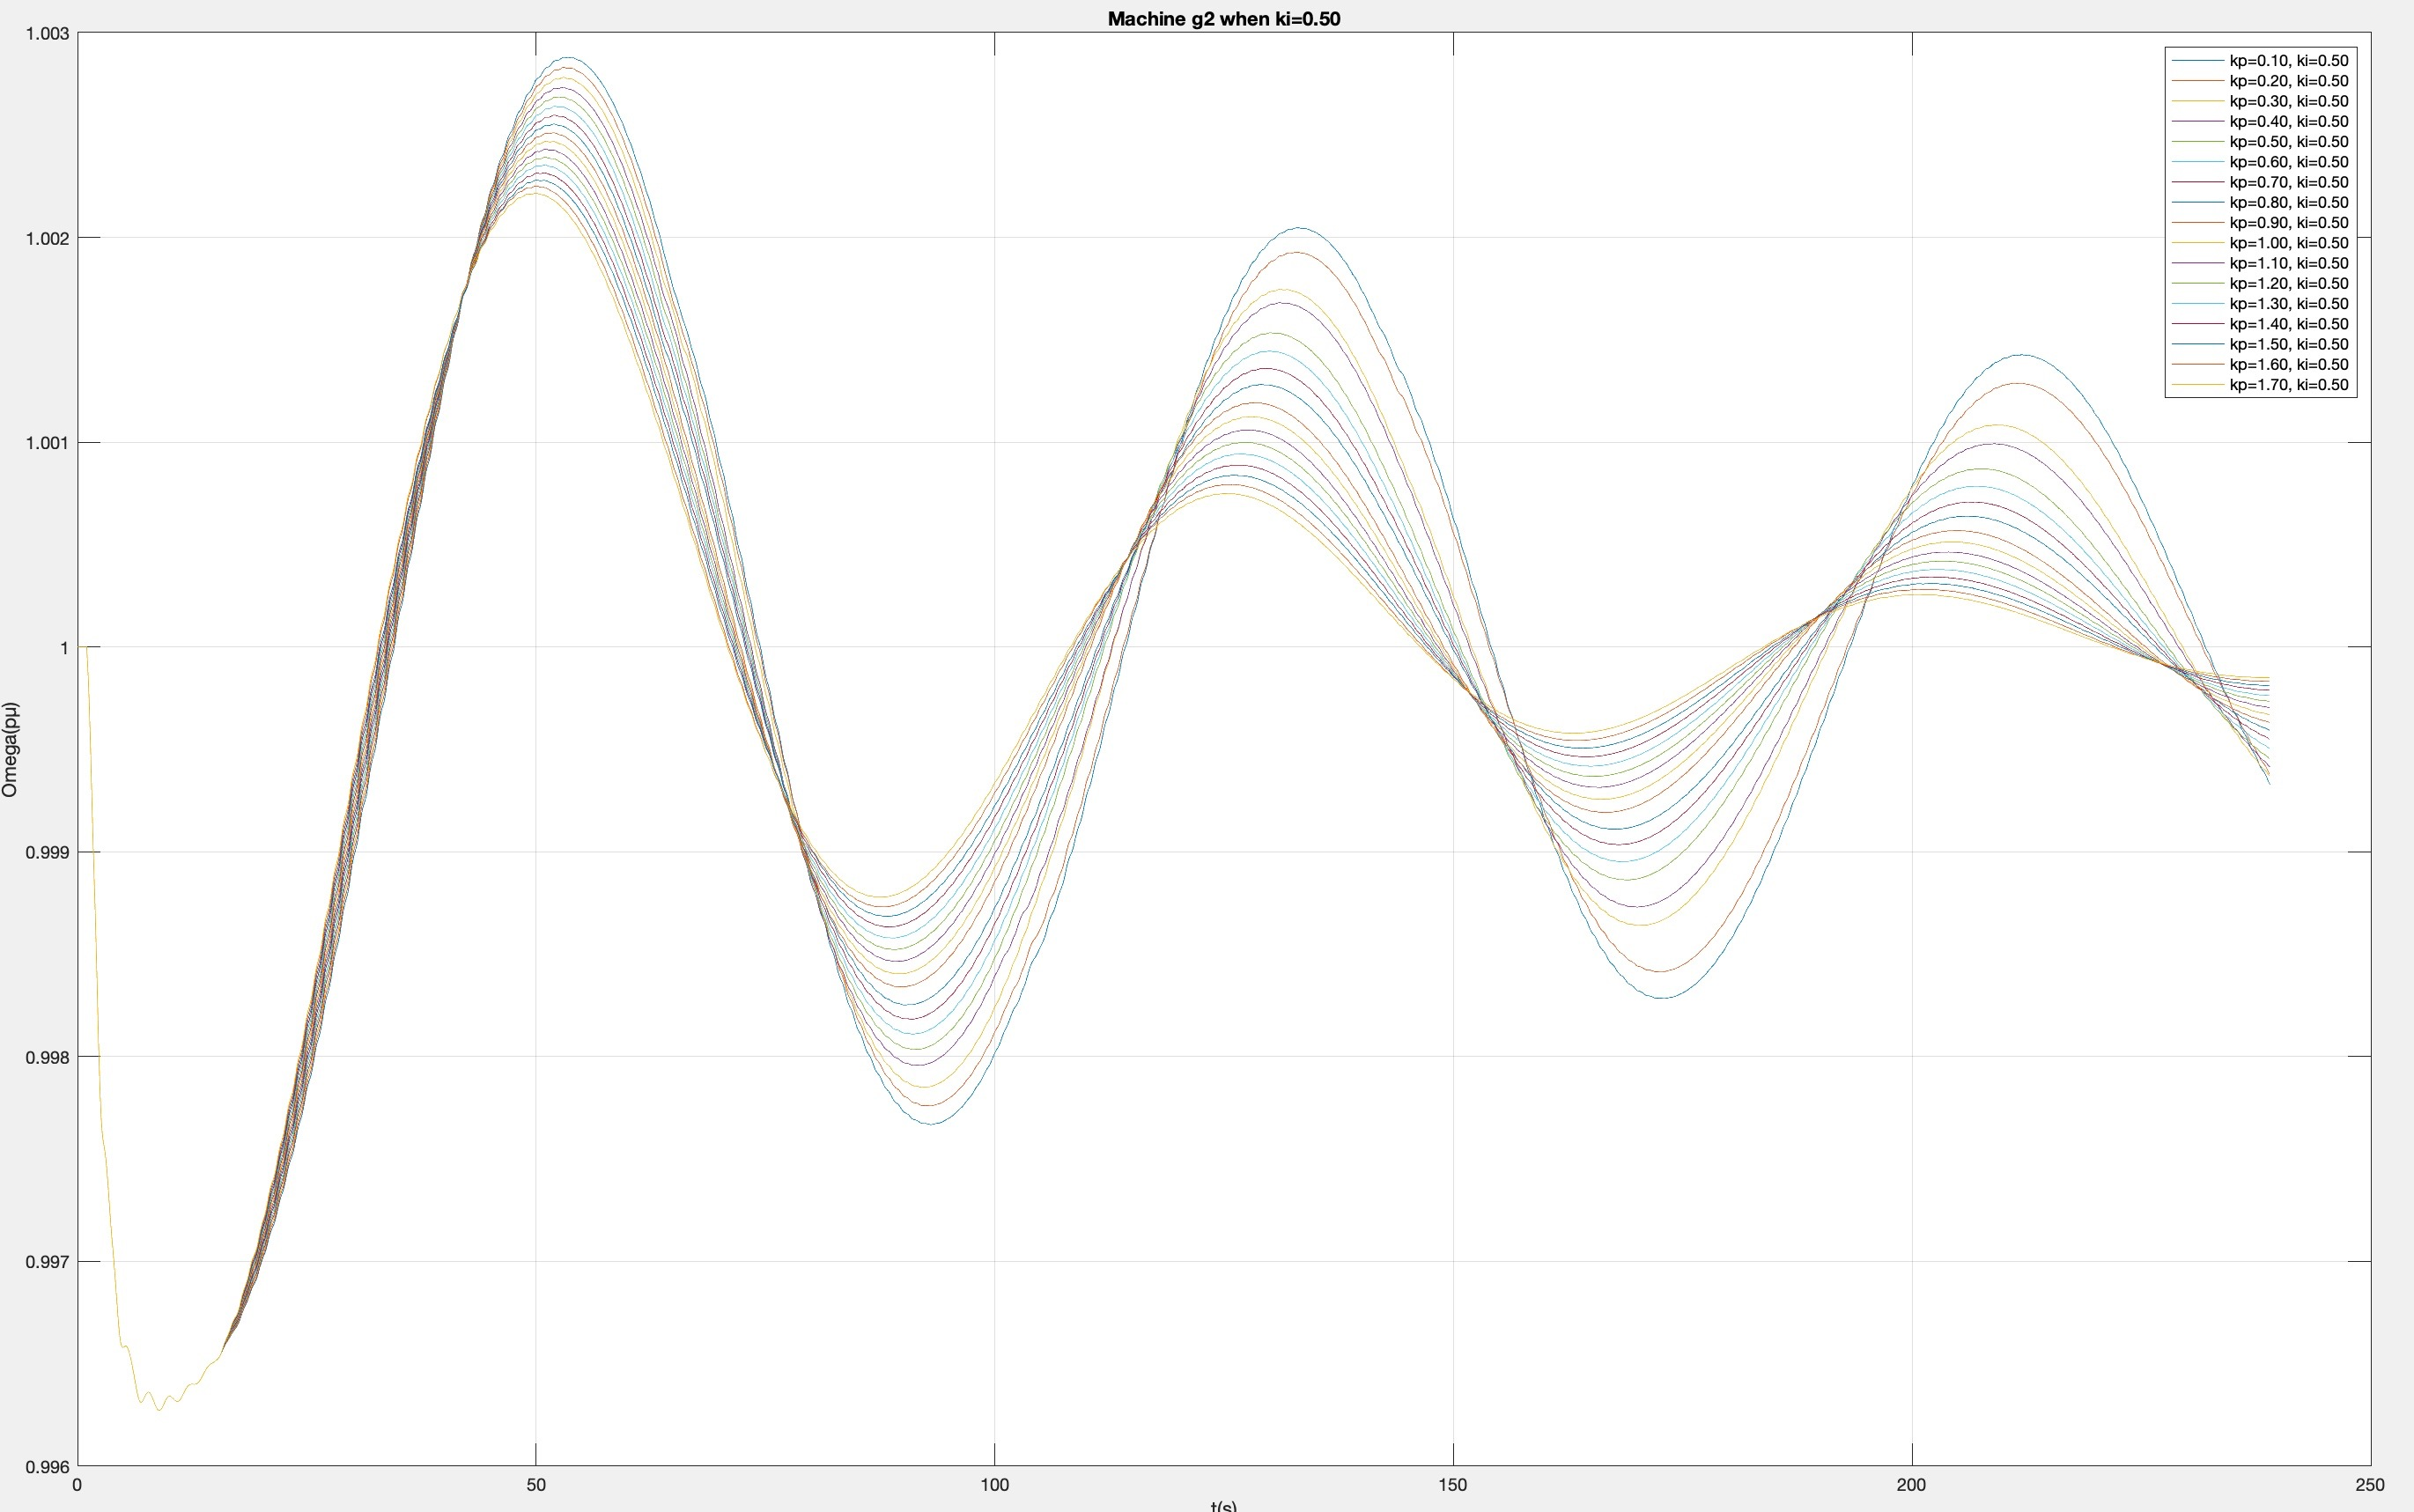
\includegraphics[width= \linewidth]{figure/3_4_1_tune_ki_2.jpeg}
  %\caption{A really Awesome Image}\label{fig:awesome_image2}
\endminipage\hfill
\minipage{0.33\textwidth}%
  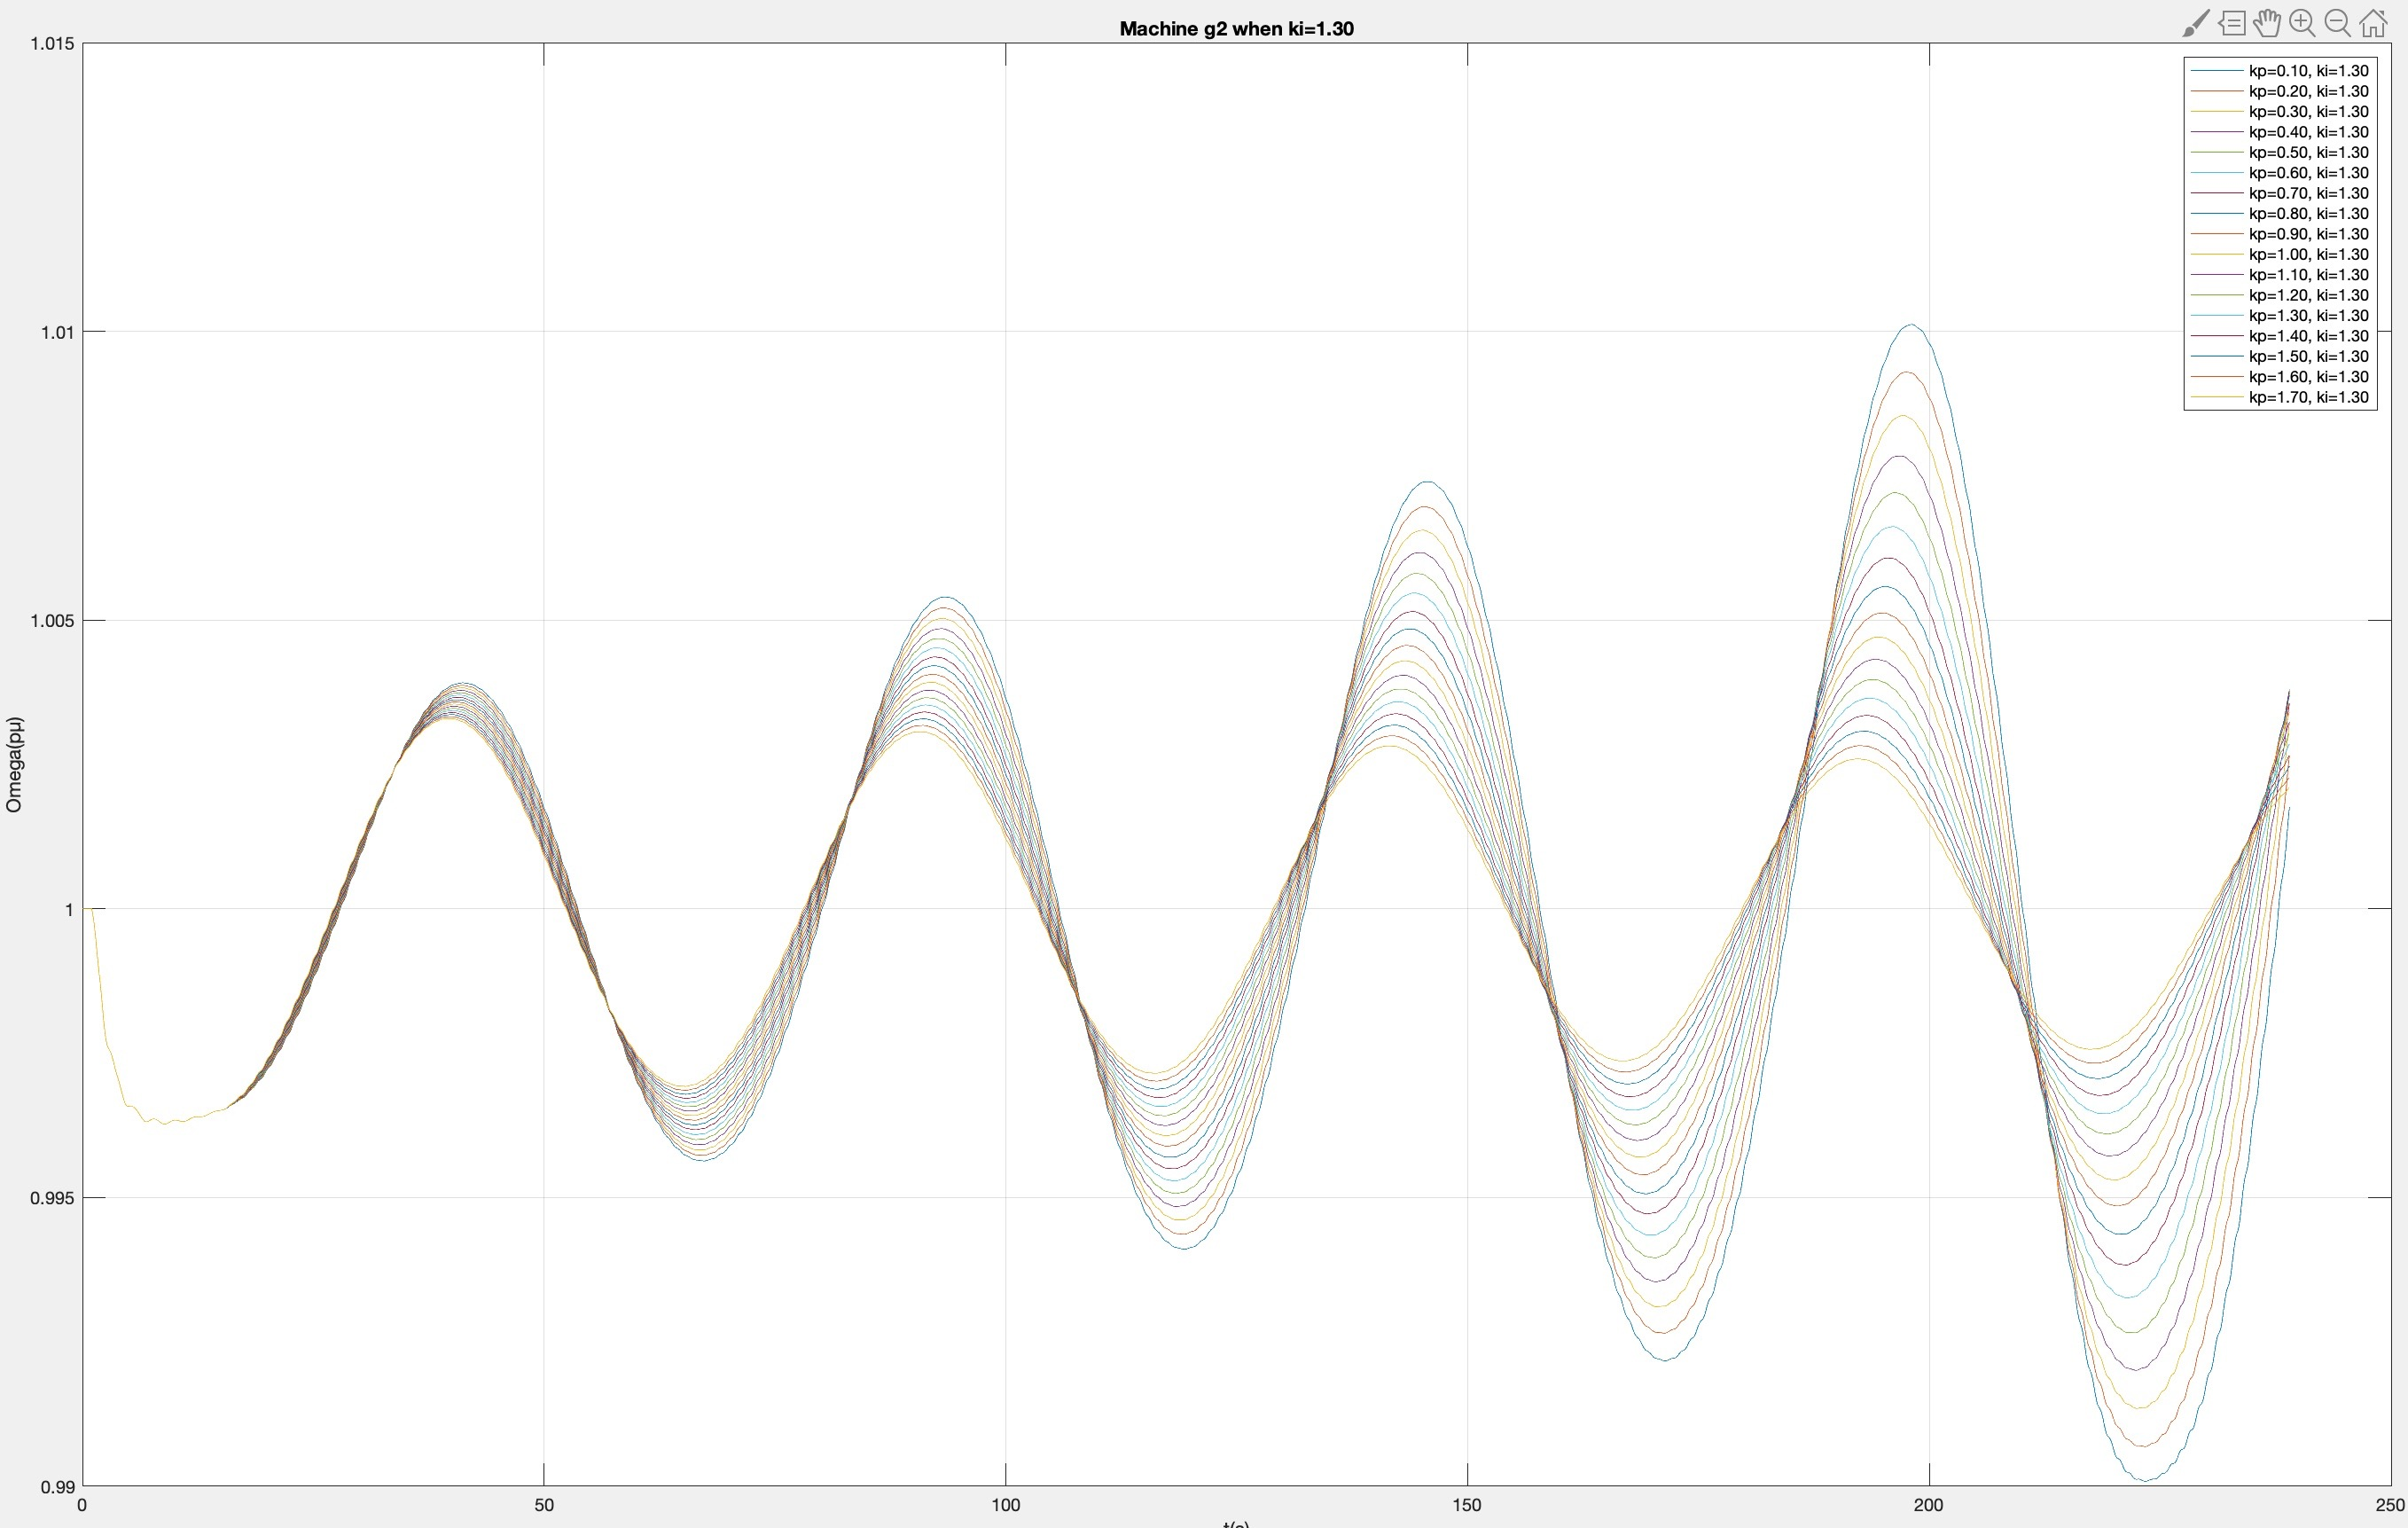
\includegraphics[width= \linewidth]{figure/3_4_1_tune_ki_3.jpeg}
  %\caption{A really Awesome Image}\label{fig:awesome_image3}
\endminipage
\caption{PI Control: ki = 0.2; ki = 0.5; ki = 1.3.}
\label{3_4_1_larger_ki}
\end{figure}


The reason for this is that neither kp nor ki can be infinitely magnified. Kp is the amplifier factor of D-term and it represents how quickly an error can be corrected. If kp is larger, the overshoot of the corrected signal will be larger. Kp has a limit because there is an acceptable range of frequency with official document. For instance, in Nordic test case scenario, the limit is ±0.2\%. In other words, the range of signal is from 0.998 $p\mu$ to 1.002$p\mu$. 

Ki is the amplifier factor of the I-term. The signal has too many oscillations and it would not be settled if we keep increasing the value of ki.

However, the signal needs to be settled before a specific time in reality and it makes sure the signal has no chance of excessive oscillation. Thus, ki is limited. 

One of the objectives of this project is to find the best combination of amplifier factors, i.e. kp and ki. To obtain it, we need to find the limit of kp and ki and simulate possible situations in the range. 

The idea of bisection method is used to find the limit of kp and ki. 

Firstly, we tune a large kp, and we test if a new signal is acceptable. To simplify the model, we choose ki being from 0.1 to the value of kp and the step of ki is dependent to the value of kp. For instance, if kp is 500.1, the range of ki is between 0.1 and 500.1. From the part we discussed before, the signal has great chance to have a large overshoot. Thus, ki can be given a large step, like 100.0. We do not need to worry about such a large step will filter some acceptable results. The purpose of this step is not to find all the acceptable results. The purpose of tuning kp and ki is not finding all the possible values. We hope to find a general relationship between kp and ki and it will be helpful to find the impact of time delay afterwards. 

Secondly, we check if the signal is acceptable if we have simulated data. The purpose of this step is to find the limit of ki. 

If ki exists (i.e. there is one acceptable result at least), for instance, ki equals to 200.1, we need to make sure there are no solutions when increasing ki by its step. Then, we can judge that the limit of the kp is between (200.1 and 200.1 + the step of kp). Thus, we have a range of kp which is between (0.1 and 200.1 + the step of kp). If the step of kp is 10, the range of kp will be from 0.1 to 210.1. Normally, we can directly tune kp and ki between 0.1 and 210.1. 

If ki exists in another way, for instance, kp equals to 200.1 and ki equals to 5.1 when the step of ki is 5.0. The result is acceptable but we need to increase the value of kp to make sure ki does not exist when kp equals to (kp + the step of kp). 

If ki does not exist, for instance, there is no acceptable ki when kp is 500.1. According to bisection method, we can test the simulations and tune kp between 0.1 and 250.1. We repeat the method above until we find the limit of kp and ki. 


\subsection{Analytical Models} %3.4.2
\label{subsection3.4.2}

The first analytical model generates two different kinds of excel files. One of them is named as ori.xlsx. This is a file saving all the acceptable results. For another kind of files, their names are related to the value of time delay. For instance, if time delay is 0.01 seconds, the file name be td\_0.01s\_xlsx. It stores all the acceptable results when delay is 0.01 seconds. 

Importantly, we define 'SettlingTimeThreshold', a MATLAB variant, to 0.02, so the time taken for the error between the response and the steady-state response will fall within 2\% of nominal value. 

\begin{figure}[htbp]
\centering
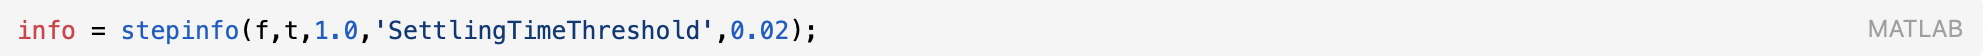
\includegraphics[width = .999\textwidth]{figure/3_4_2_code4.png}
\caption{MATLAB: stepinfo function.}
\label{3_4_2_code4}
\end{figure}

In our case, the system starts from the zeroth second. However, in the analytical model, we can not put all the data into the stepinfo function because the data should be analysed from the beginning of SFC. Thus, the data stepinfo function gets should starts from the SFC control starting, which is the 150th seconds.  

\begin{figure}[htbp]
\centering
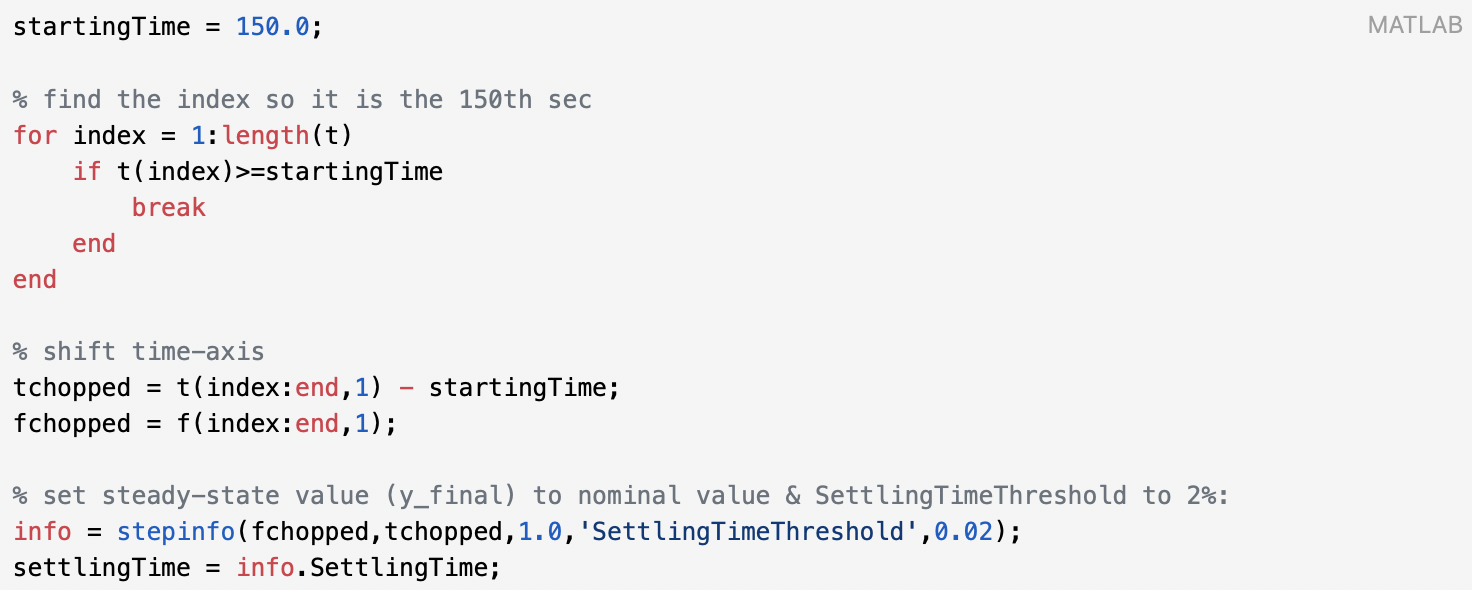
\includegraphics[width = .999\textwidth]{figure/3_4_2_chopped.png}
\caption{MATLAB: chopped the time from the 150th sec.}
\label{3_4_2_chopped}
\end{figure}


In the first analytical model named i\_cur\_plot.cur , we check if simulation results are acceptable via our MATLAB program if we have collected data. Firstly, we import data from simulations. Then, we limit both the overshoot and settling time as required via a MATLAB module: stepinfo. The data will be filtered if the overshoot or the settling time is not in the required range. 

\begin{figure}[htbp]
\centering
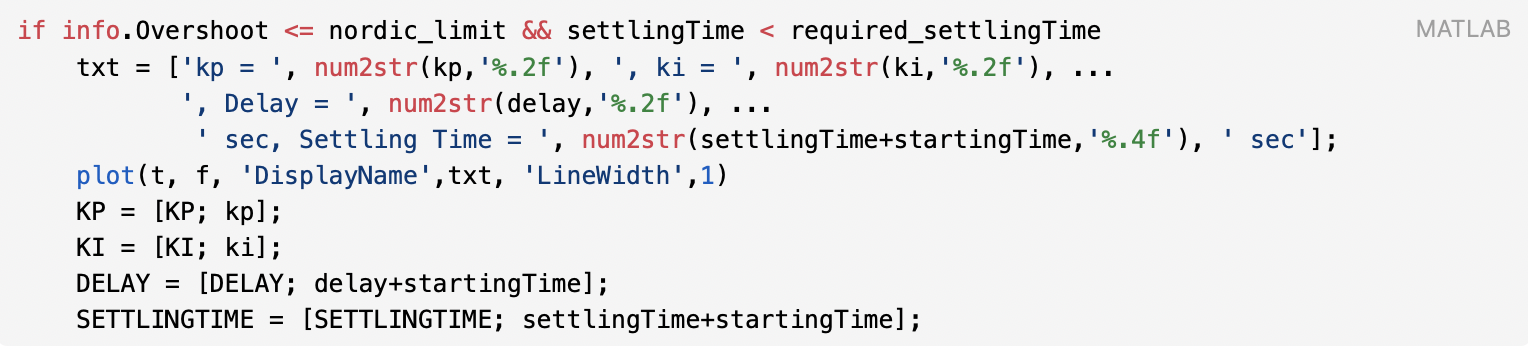
\includegraphics[width = .999\textwidth]{figure/3_4_2_code5.png}
\caption{MATLAB: filter unacceptable tuning results.}
\label{3_4_2_code5}
\end{figure}


As you can see from Figure~\ref{3_4_2_code5}, if the signal is acceptable, its parameters, i.e. kp, ki and time delay, will be saved in prepared lists. The lists will be transferred into the two kinds of excel files. 

The second analytical model helps finding which combination of kp and ki has a minimum settling time with a fixed delay. The idea is as follows. Firstly, we import an excel file, whose name is related to the value of delay,  that is generated by the last step. Then, we find the minimum settling time. Finally, we find related kp, ki and delay and export them into another excel file. 

The third analytical model helps finding the best combination of kp and ki. Firstly, we import data from ori.csv. Then, we calculate the average settling time for each combination of kp and ki. However, it is invalid that a combination is not acceptable for all the time delay. Thus, we need to add a limitation factor to make sure the best combination is valid for every delay. For instance, if there are 21 different time delays, we can use 

\begin{figure}[htbp]
\centering
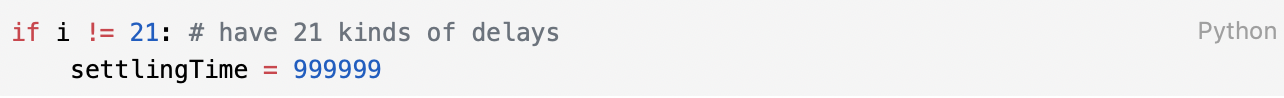
\includegraphics[width = .999\textwidth]{figure/3_4_2_code6.png}
\caption{Python: filter out the tuning results that cannot settled in all delay}
\label{3_4_2_code6}
\end{figure}

to filter some unacceptable results. Finally, we have all the average settling time so we can find the minimum average settling time. 

The fourth analytical model helps sorting out the combination’s settling time with different time delay. It is one of the inputs of the fifth analytical model. 

The fifth analytical model helps plotting a 3D triangle surface diagram. It draws a 3d plot from the data in ori.xlsx. We use: 

\begin{figure}[htbp]
\centering
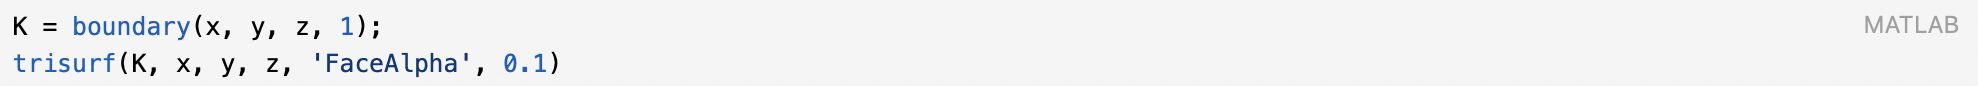
\includegraphics[width = .999\textwidth]{figure/3_4_2_code7.png}
\caption{MATLAB: 3D triangle surface algorithm.}
\label{3_4_2_code7}
\end{figure}

to draw a triangle surface plot. Besides, it highlights the results from the second analytical model and the fourth analytical model. With a 3D triangle surface plot, we can clearly understand the impacts of the time delay. 
\section{Rate of Generators Change} %3.5
\label{section3.5}
Generators have a limit on the output power (in MW) and another limit on the rate of change of power (in MW/minute). The rate of change of power is called ramp rate. It expresses how quickly a power plant's power output is changing. 

\begin{equation}
    Rate = \frac{\Delta P}{\Delta t}
\end{equation}


According to National Renewable Energy Lab., Golden, CO (US), \cite{osti_15016292} large thermal units are usually able to ramp around 1\% of their capacity per minute. For instance, if a generator's nominal power is 360 MW, its ramp rate will be 3.6 MW/min or 0.06 MW/sec.\\

In this project, benefiting from \sys{pyramses}~\footnote{\sys{pyramses} is a Python library for \sys{RAMSES} dynamic simulator: \href{https://anaconda.org/apetros/pyramses}{https://anaconda.org/apetros/pyramses}}, it's possible to get generators' power output directly from the simulator. Thus, through the MATLAB \sys{stepinfo}~\footnote{\sys{stepinfo} contains \sys{Rise time}, \sys{settling time}, and other step-response characteristics. Document: \href{https://www.mathworks.com/help/control/ref/stepinfo.html}{https://www.mathworks.com/help/control/ref/stepinfo.html}} module, we can use \sys{Peak} and \sys{PeakTime} to calculate the ramp rate:

\begin{equation}
    Rate = \frac{P_{\sys{peak}} - P_o}{\sys{PeakTime}}
\end{equation}

where $P_o$ is the original power output of a generator when SFC starts (i.e. $P_{t=0}$ when the SFC starts).\\

I have to explain why I don't use \sys{RiseTime} to calculate the ramp rate. It seems like \sys{RiseTime} ensures the rate's reliability from its definition: "Time it takes for the response to rise from 10\% to 90\% of the steady-state response". However, unlike frequency, generators do not have steady-state response ($y_{final}$). Traditionally, we can use the final value of the signal as steady-state response ($y_{final}$). However, in this case, as shown in Figure~\ref{3_5_yfinal1} and in Figure~\ref{3_5_yfinal2}, different tuning results may bring different $y_{final}$. It makes using $y_{final}$ as steady-state response nearly impossible. Choosing \sys{Peak} and \sys{PeakTime} that are not related with steady-state response is necessary.

\begin{figure}[!t]
\center
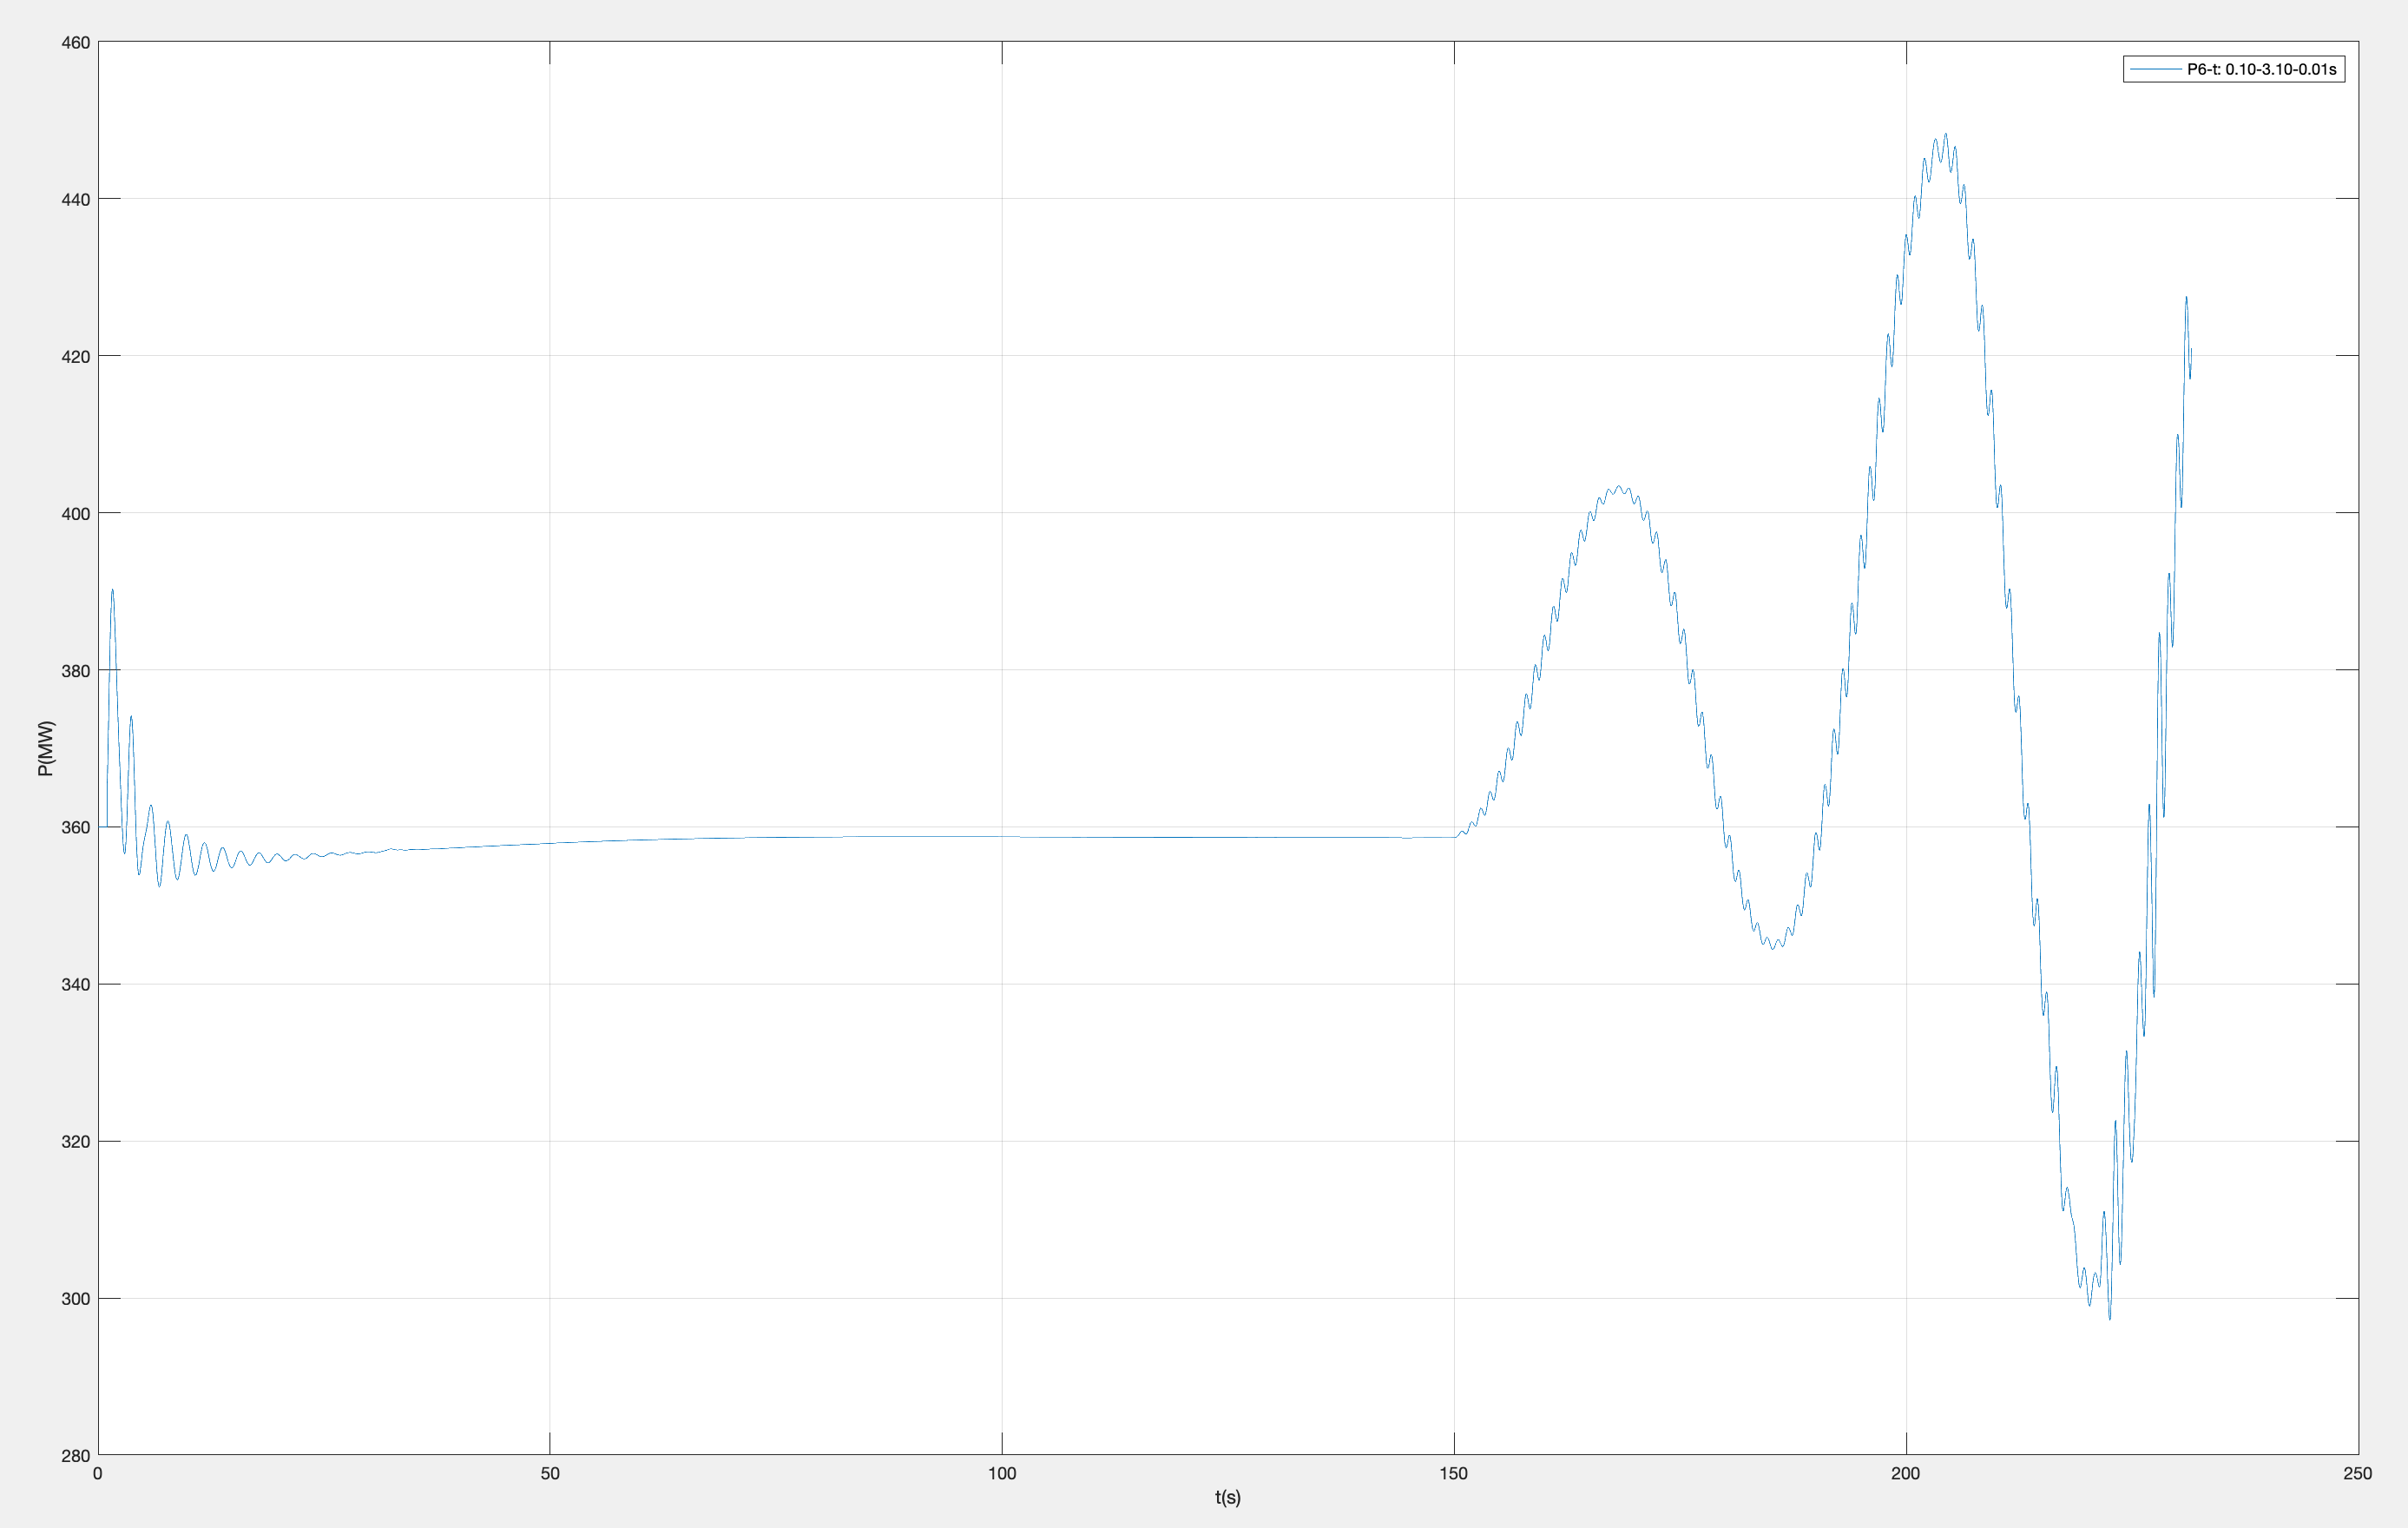
\includegraphics[scale=0.25]{figure/3_5_yfinal1.png}
\caption{g6's power output: kp=0.1, ki=3.1}
\label{3_5_yfinal1}
\end{figure}

\begin{figure}[!t]
\center
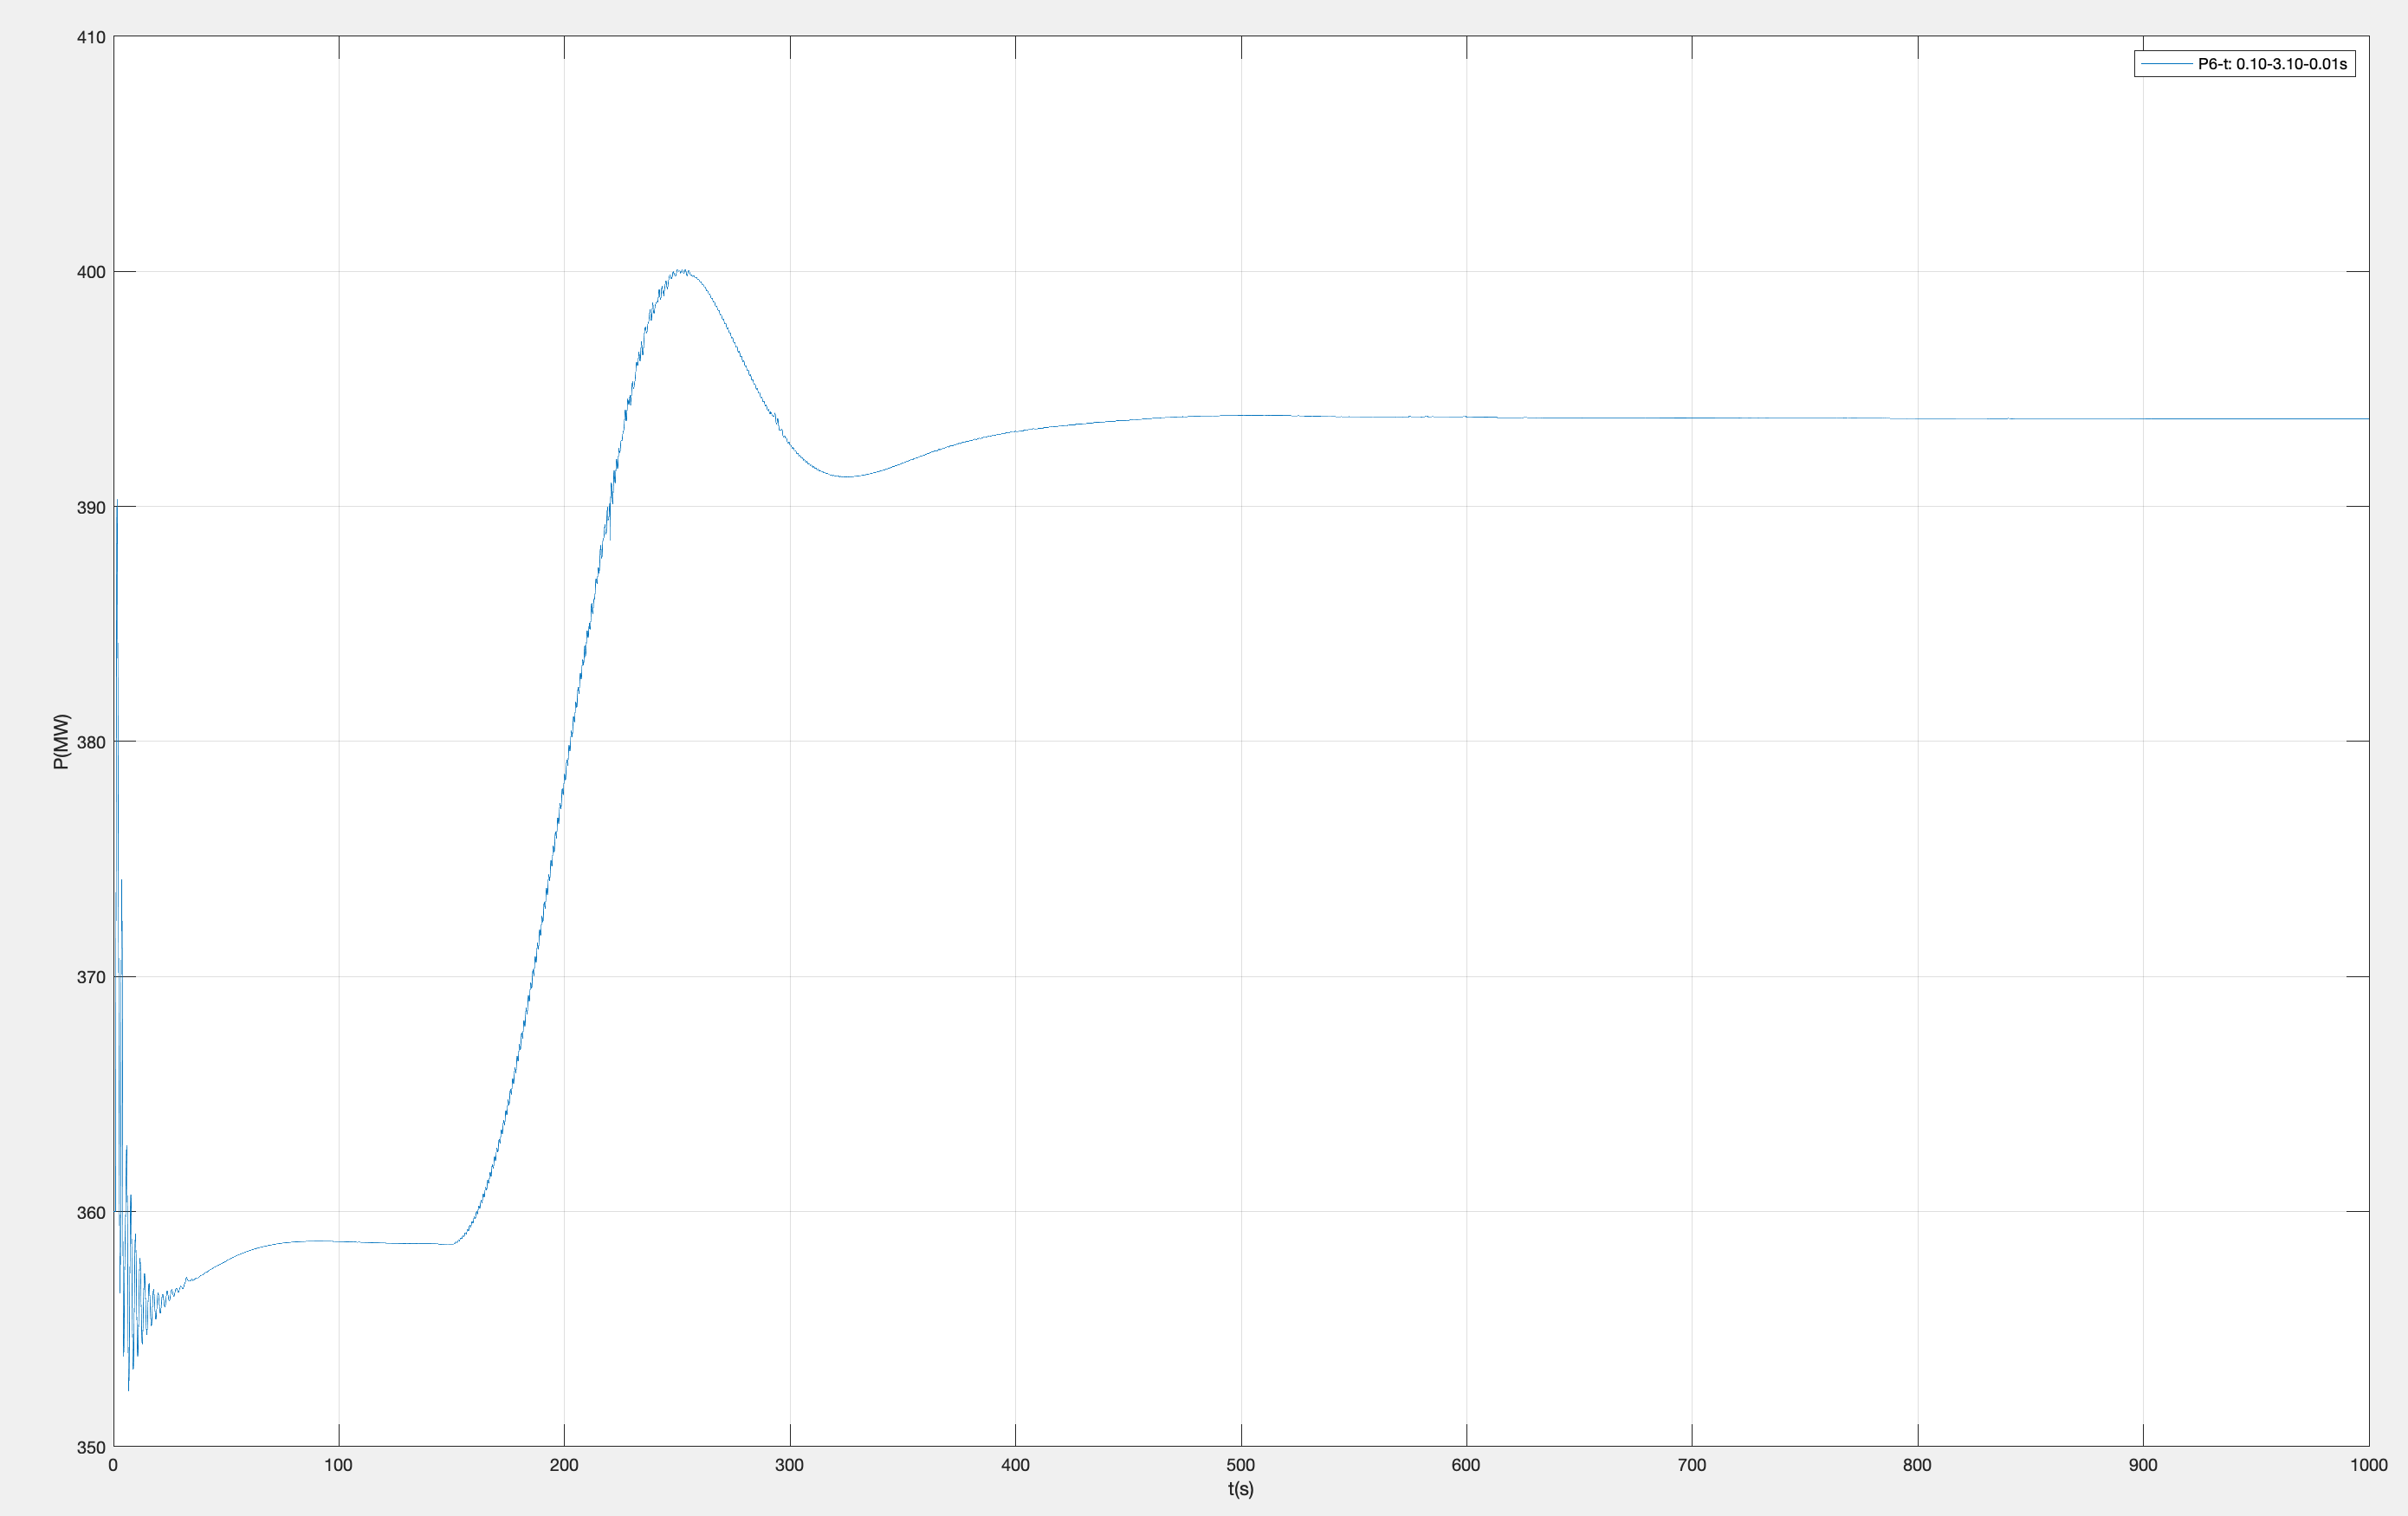
\includegraphics[scale=0.25]{figure/3_5_yfinal2.png}
\caption{g6's power output: kp=0.1, ki=0.1}
\label{3_5_yfinal2}
\end{figure}




% PART II
\part{Test Case Scenario (Nordic)}

\chapter{Low Time Delay}
\label{Chapter4}
% section:
\section{Hypothesis} %4.1
\label{section4.1}
\subsection{Hardware Hypothesis} %4.1.1
\label{subsection4.1.1}

In this Chapter, we use the algorithms described in the Chapter~\ref{Chapter3} to test the well-known Nordic system. One-line diagram of the Nordic test system is  shown in Figure~\ref{4_1_1_nordic}. 

\begin{figure}[htbp]
\centering
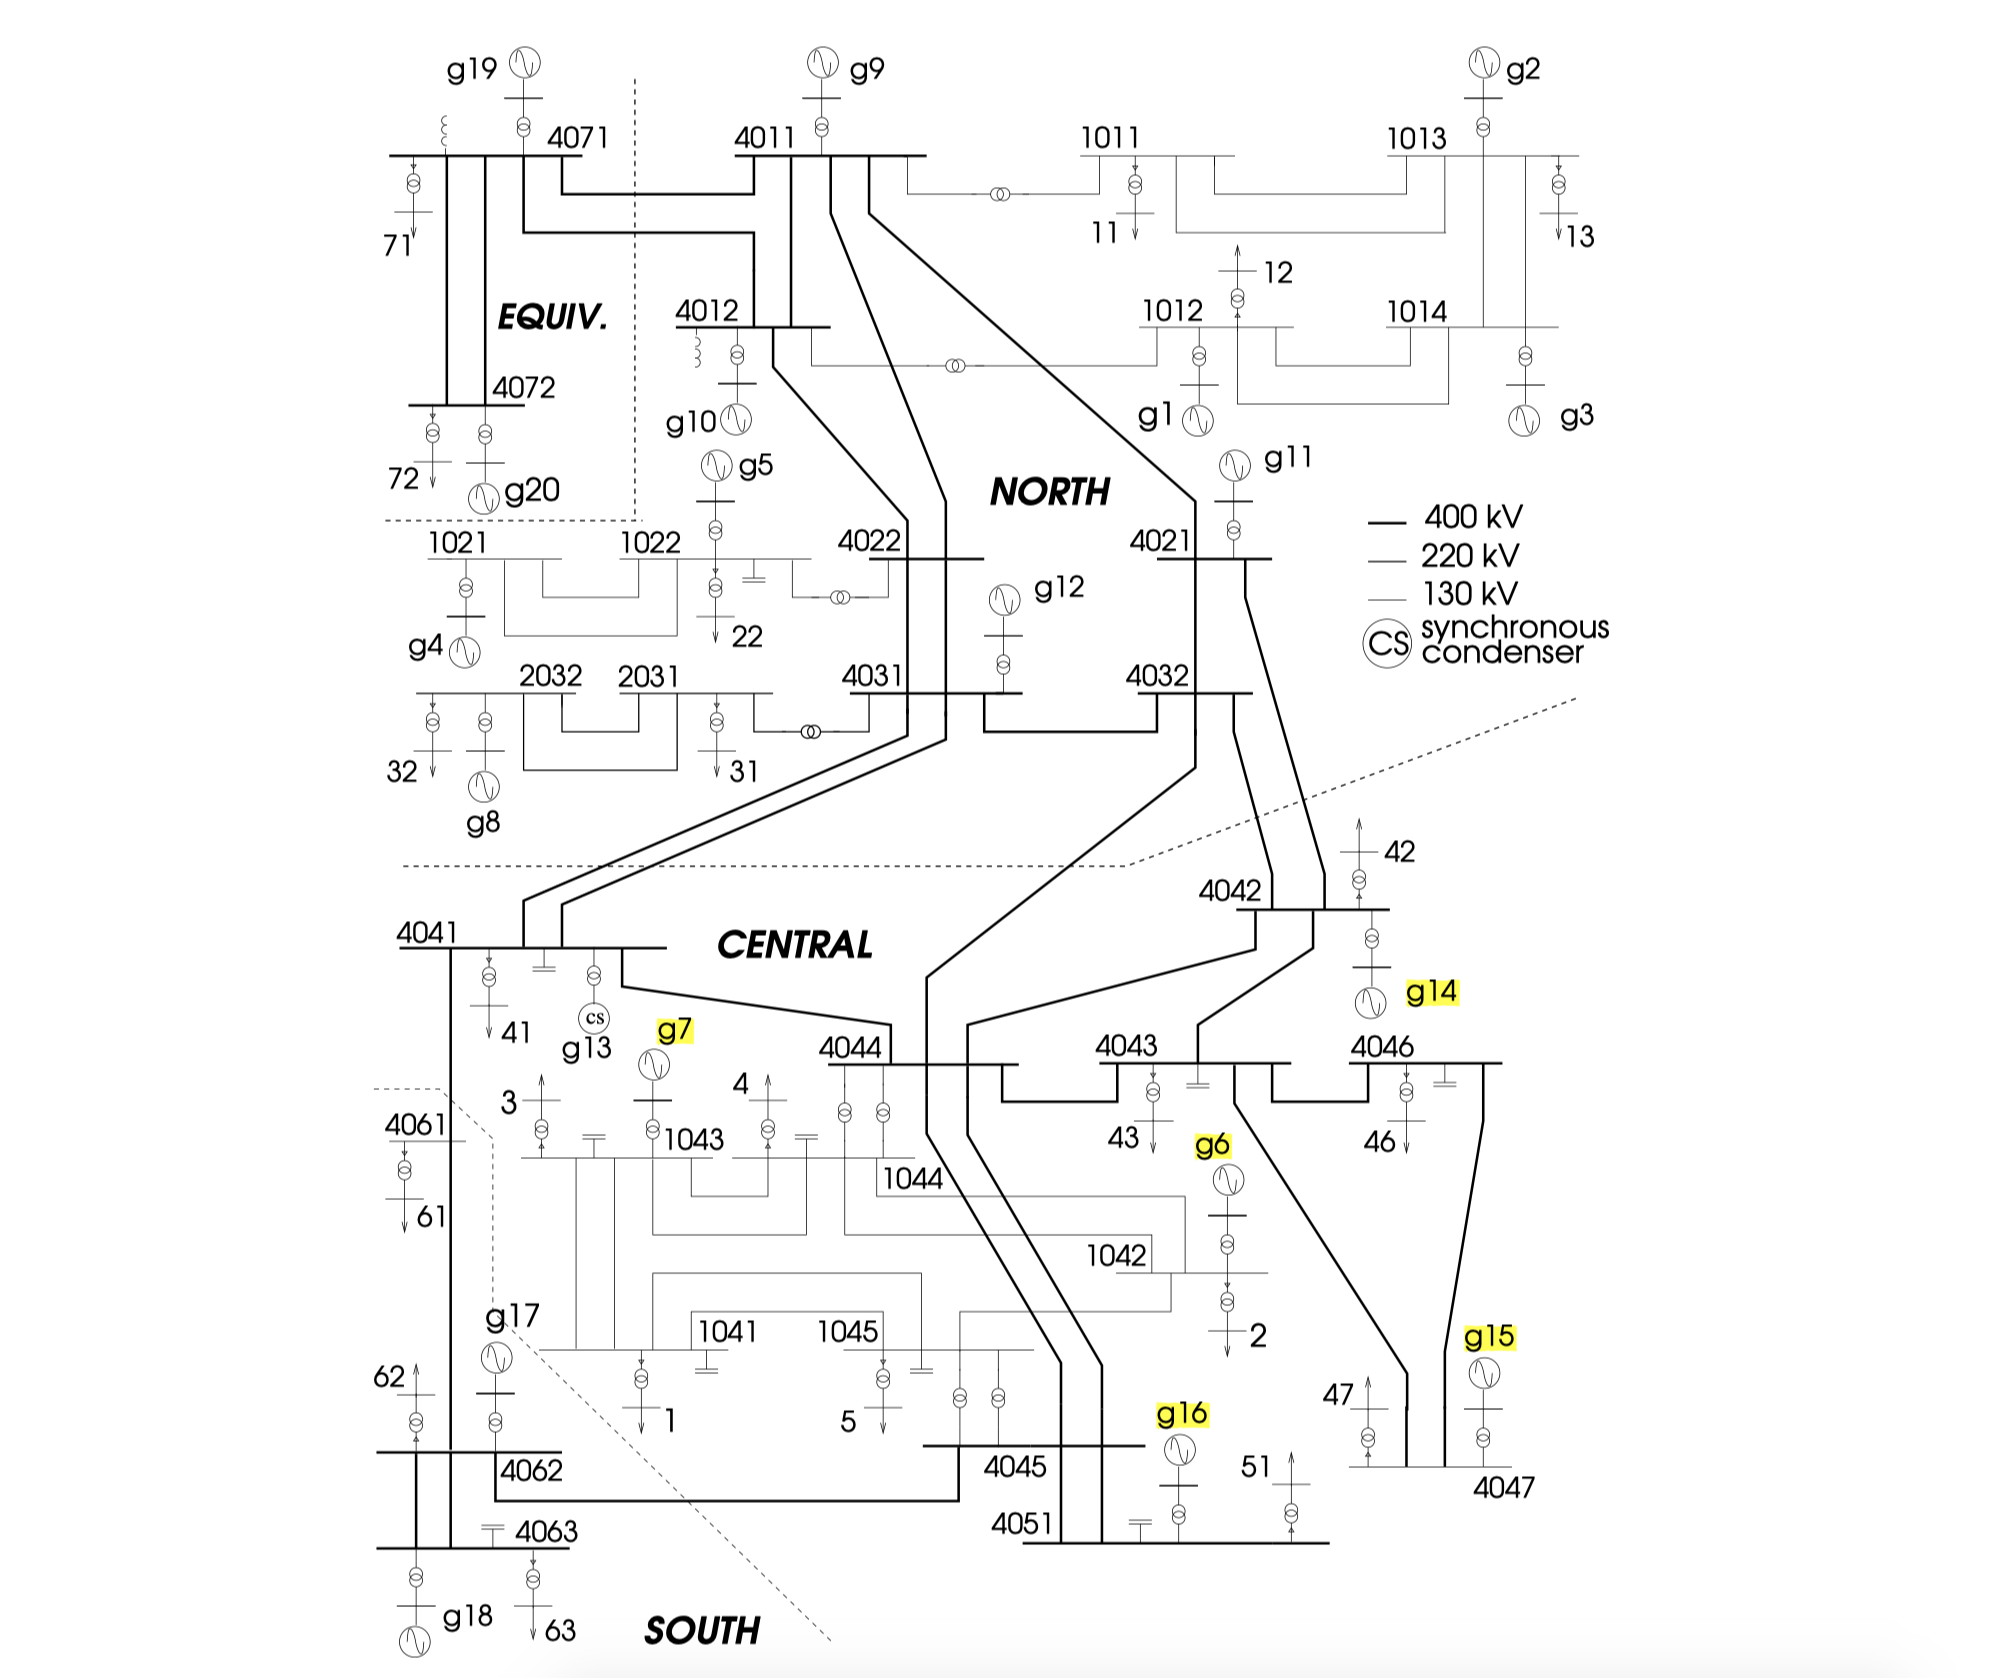
\includegraphics[width = .891\textwidth]{figure/4_1_1_nordic.png}
\caption{One-line diagram of the test system}
\label{4_1_1_nordic}
\end{figure}

Firstly, we assume g2 as our monitor. The monitor sends its frequency, also the frequency in the system, to the communication layer. Then, we choose five thermal generators  (g6, g7, g14, g15, g16) in the CENTRAL area. There are three reasons I choose these five generators that produce the power to the system when disturbances occur in the system. First of all, these are thermal generators not the generators in the NORTH area which are equipped with hydraulic turbines. We only have strict mathematical proof of thermal generators. Another reason is they have nice nominal power as shown the Table~\ref{nominalPower} below. The second reason is the difference of them is up to 900 MW which is good for researching the function of generators comprehensively. The last reason is I was collaborated with a PhD student. We researched Nordic test system in different algorithms. He used distributed method and I used centralised method. For convenience, we keep our generators the same. 


\begin{table}[htbp]
\centering
\begin{tabular}{ll}
Generator & Nominal Power (MW) \\
g1        & 760.0              \\
g2        & 570.0              \\
g3        & 665.0              \\
g4        & 570.0              \\
g5        & 237.5              \\
g6        & 360.0 (1/8)        \\
g7        & 180.0 (1/16)       \\
g8        & 807.5              \\
g9        & 950.0              \\
g10       & 760.0              \\
g11       & 285.0              \\
g12       & 332.5              \\
g13       & 0.0                \\
g14       & 630.0 (7/32)       \\
g15       & 1080.0 (3/8)       \\
g16       & 630.0 (7/32)       \\
g17       & 540.0              \\
g18       & 1080.0             \\
g19       & 475.0              \\
g20       & 4275.0             

\end{tabular}
\caption{Generators Nominal Power in Nordic.}
\label{nominalPower}
\end{table}

After choosing the generators, we need to choose a breaker. The breaker is a generator that can be disconnected to the system. Thus, a breaker is one of the most important impact factors to the grid system. However, at first, I am not sure how to choose a suitable breaker but then I try to disconnect all of them one by one without Secondary Frequency Control. Results are as Figure~\ref{4_1_1_without1}. 

\begin{figure}[htbp]
\centering
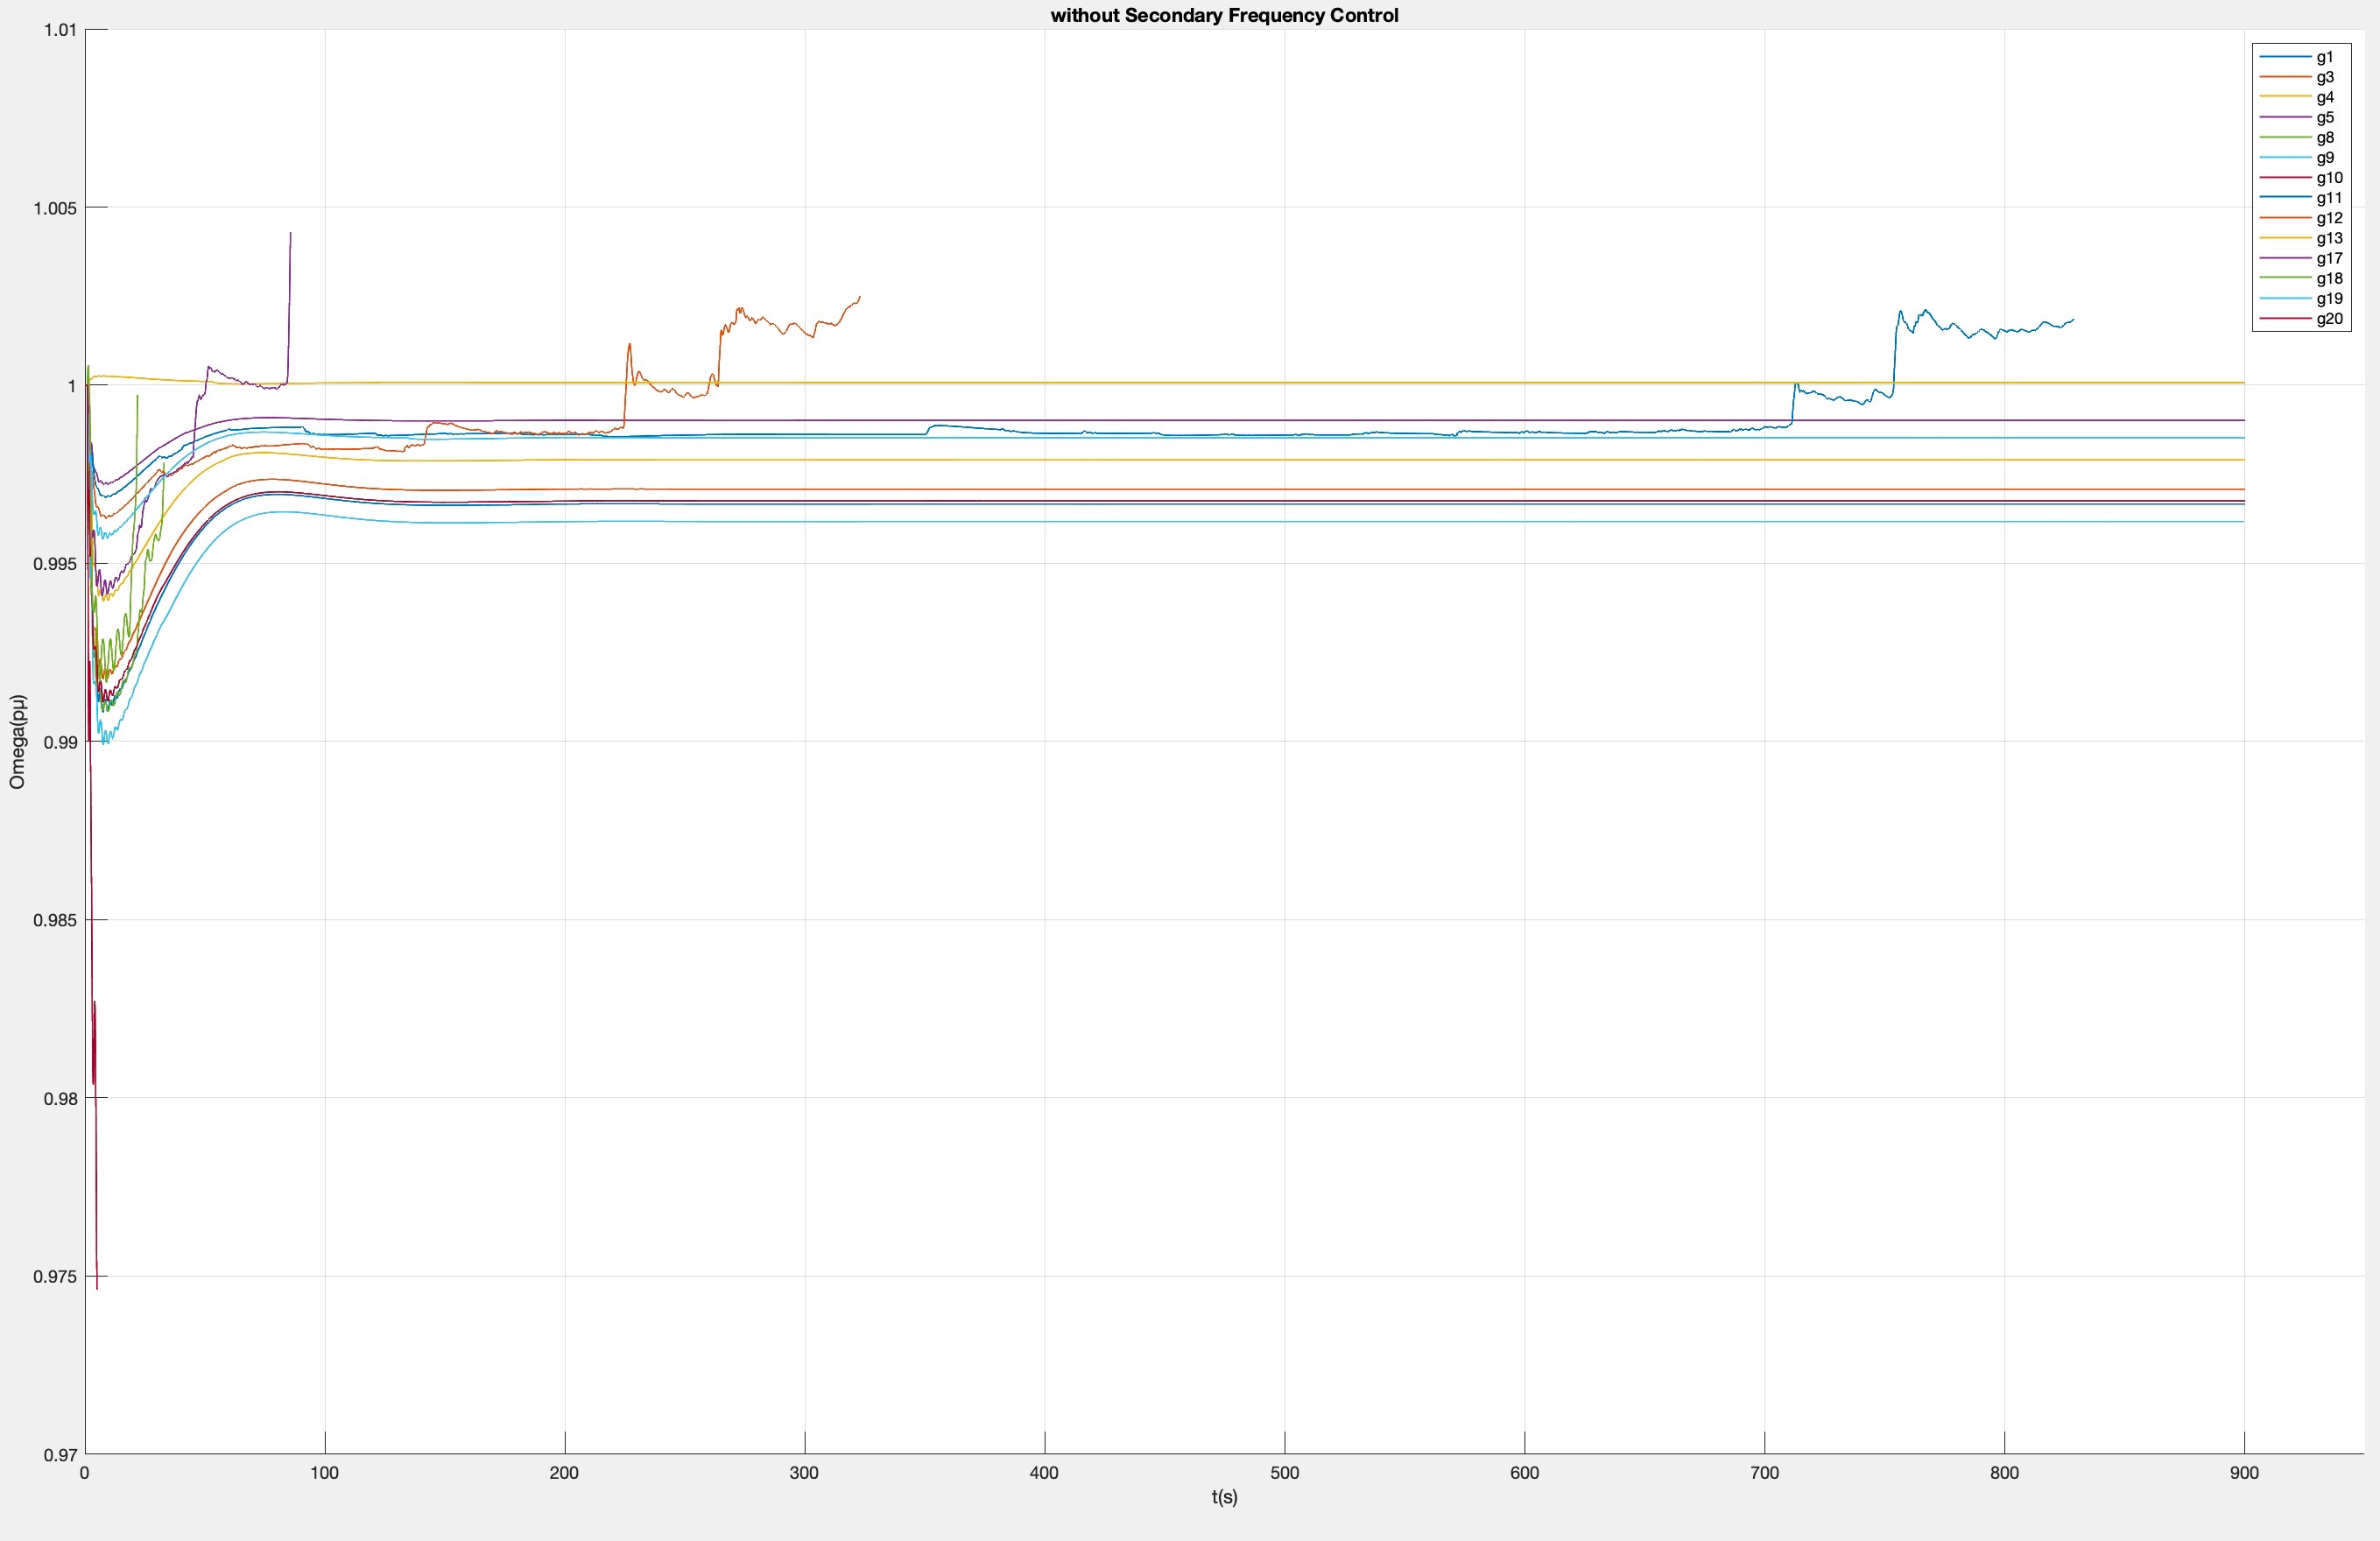
\includegraphics[width = .891\textwidth]{figure/4_1_1_without1.jpeg}
\caption{MATLAB figure: simulation results with different breakers, without SFC.}
\label{4_1_1_without1}
\end{figure}

As we can see from Figure~\ref{4_1_1_without1}, g8, g17, g18 and g20 are extremely unstable before 100 seconds and g13 have zero nominal power (because it has zero nominal power, from Table~\ref{nominalPower}). Thus, we choose a breaker out of them to make sure we have a smooth testing environment. 


\begin{figure}[htbp]
\centering
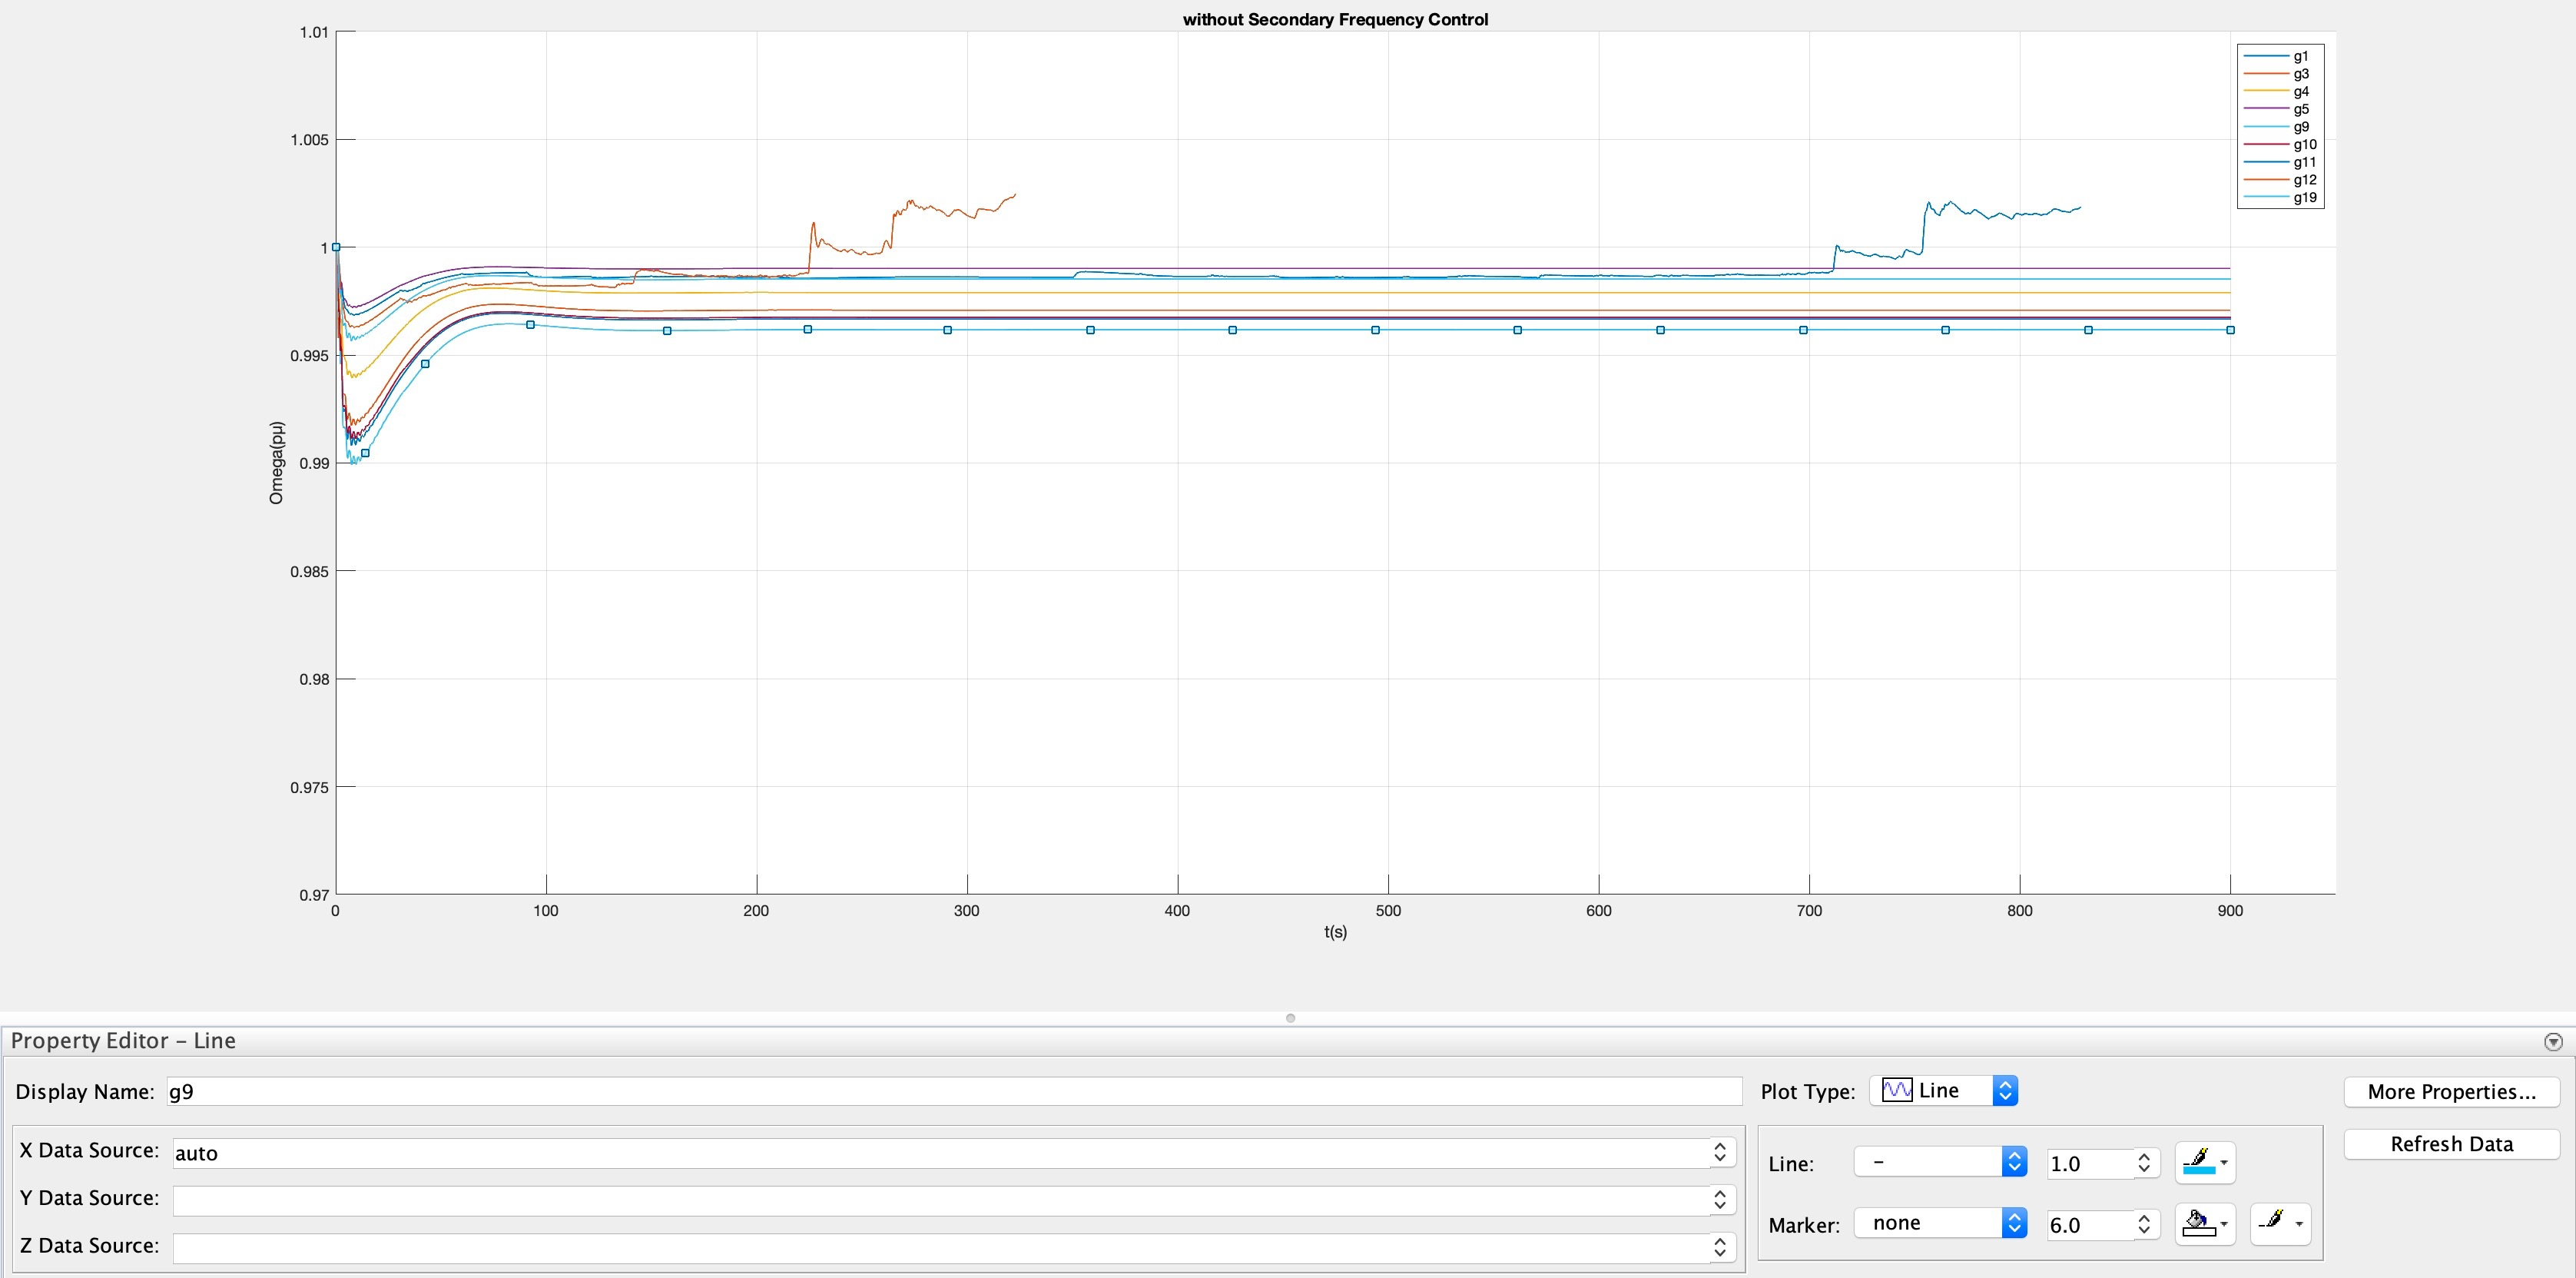
\includegraphics[width = .891\textwidth]{figure/4_1_1_without2.jpeg}
\caption{MATLAB figure: choose g9 as breaker.}
\label{4_1_1_without2}
\end{figure}

Finally, we choose g9, as shown in Figure~\ref{4_1_1_without2}, because it has a large steady-state error. Thus, the turbines will send more power to the system. It is easier to see the changes of kp and ki. 

\subsection{Software Hypothesis} %4.1.2

\begin{figure}[htbp]
\centering
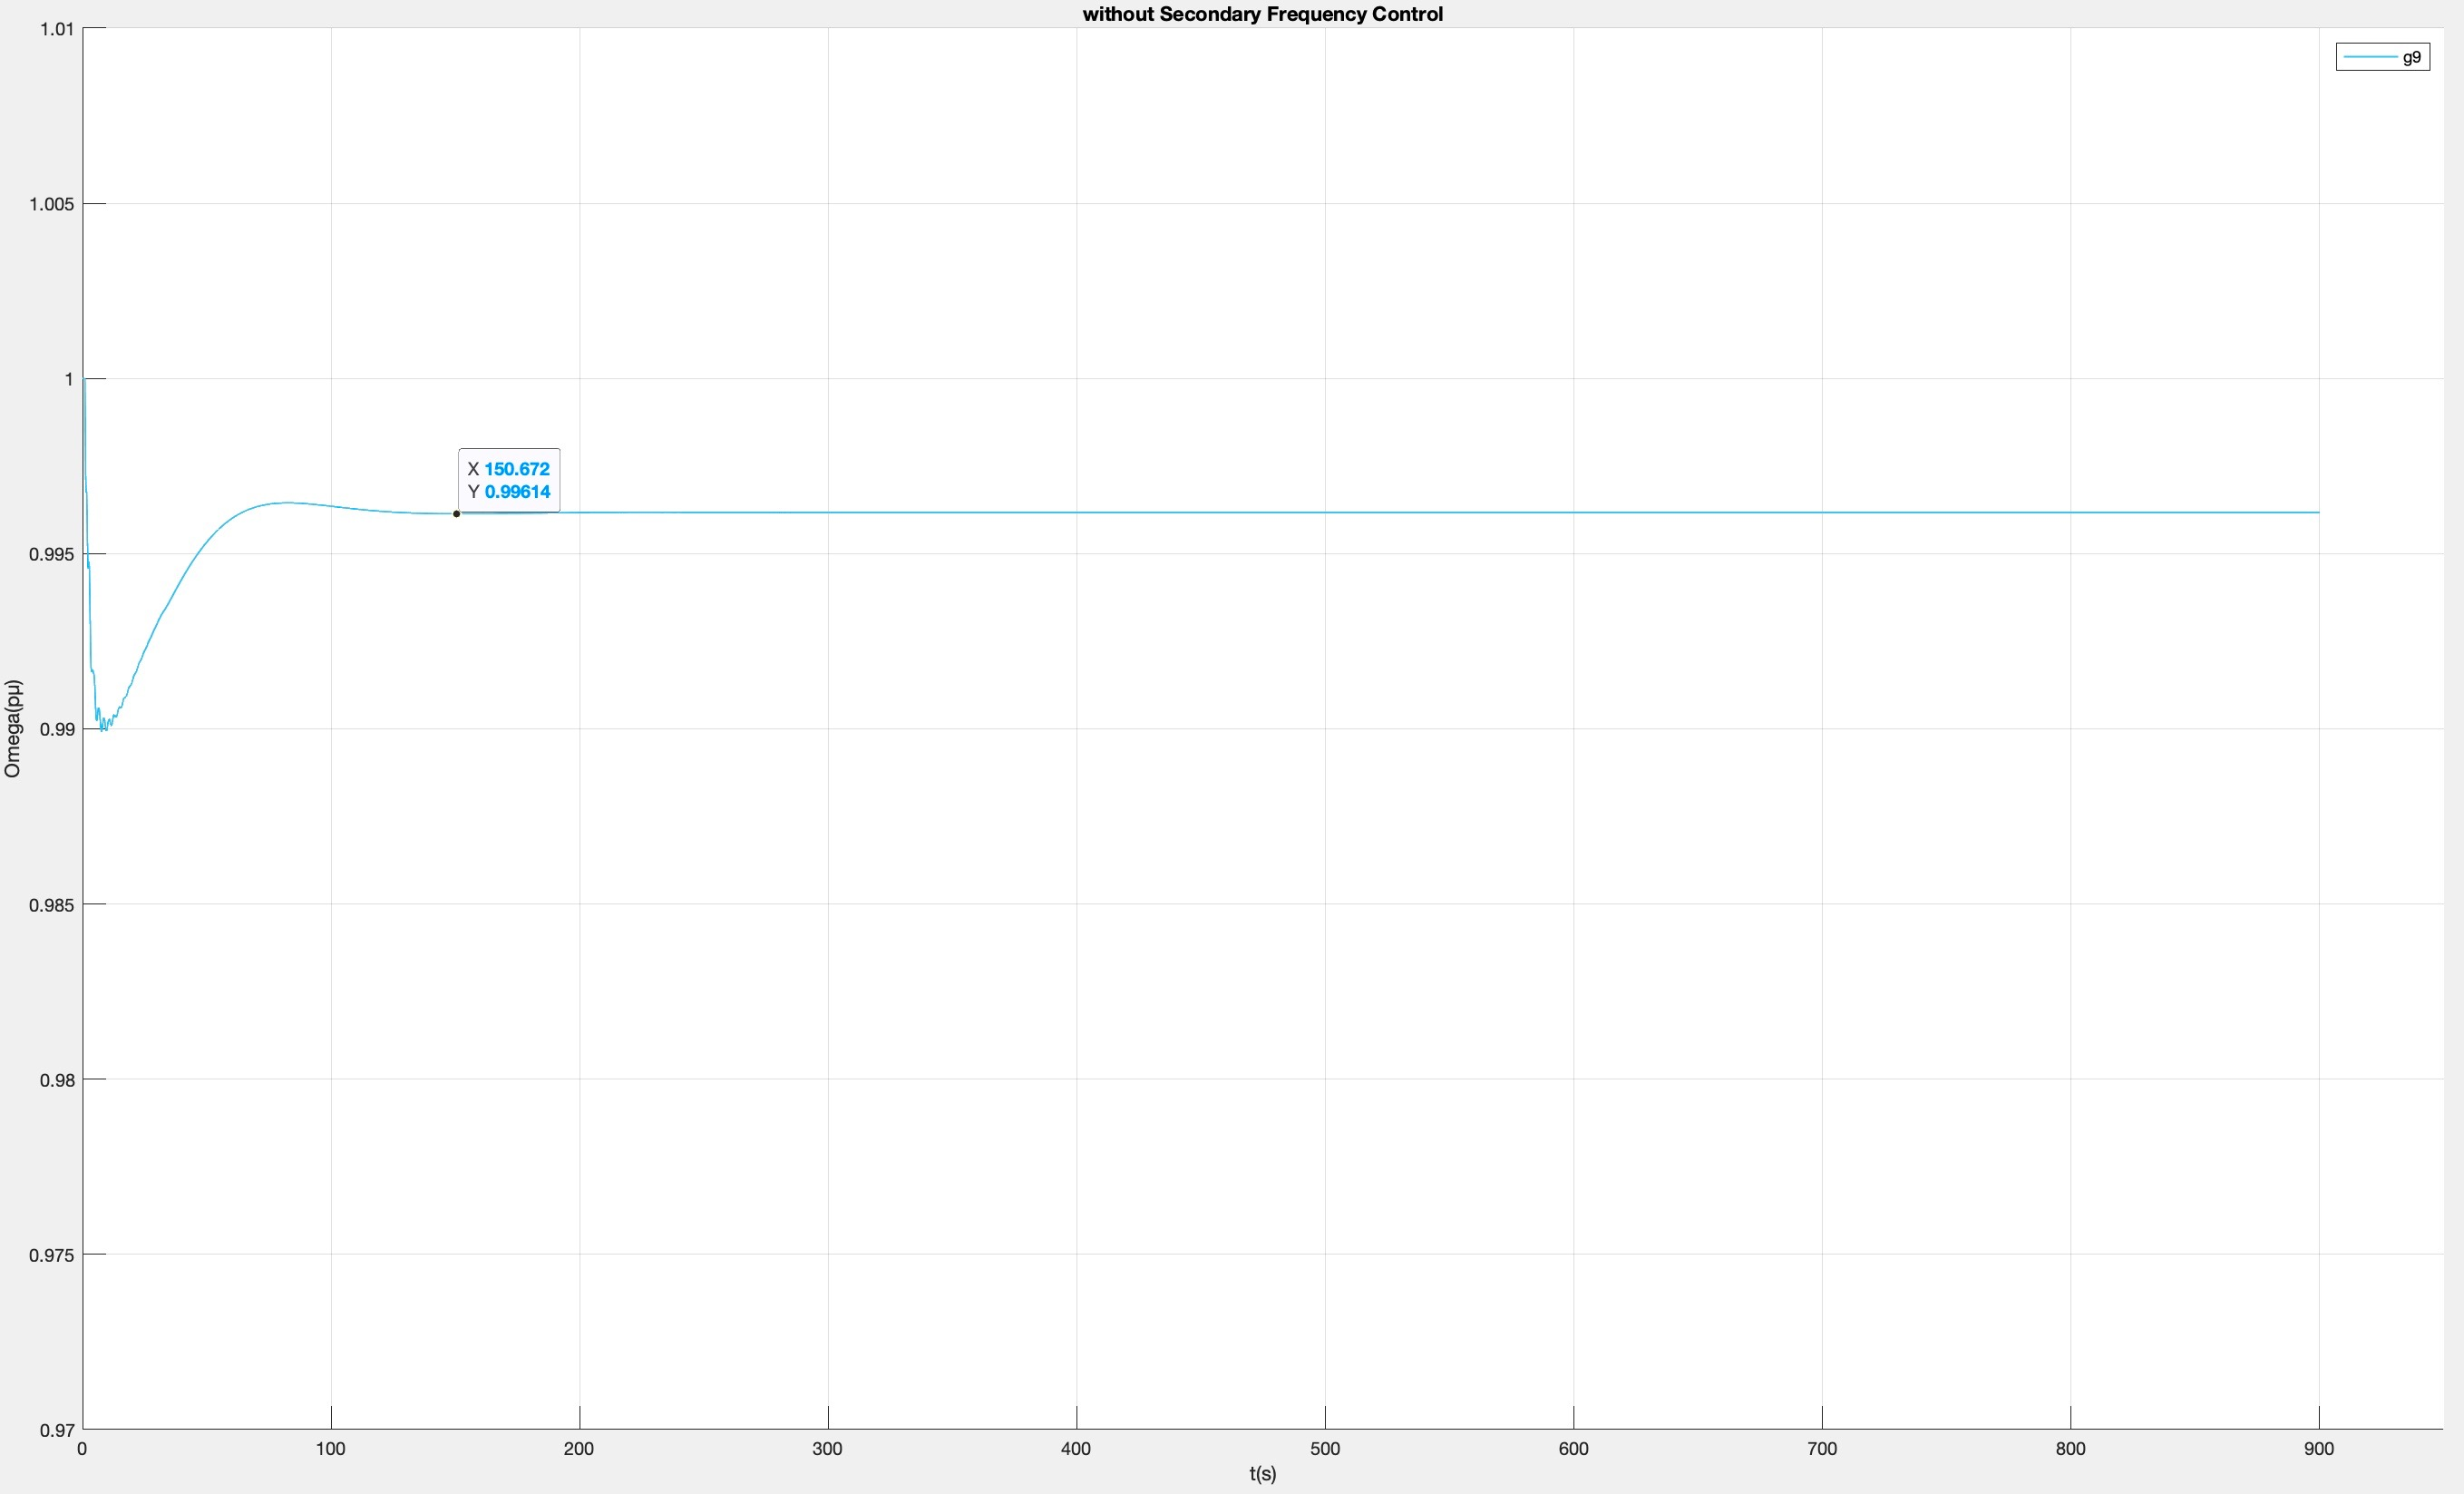
\includegraphics[width = .891\textwidth]{figure/4_1_1_without3.jpeg}
\caption{MATLAB figure: choose start time for SFC.}
\label{4_1_1_without3}
\end{figure}
Next hypothesis is about start time and end time. In the definition of Primary Frequency Control, its power balance will be restored at a lower or higher frequency, thus, from the Figure~\ref{4_1_1_without3}, we can observe that, at the 150th seconds, the frequency is stable. Thus, I choose the 150th second at the beginning of Secondary Frequency Control. In the definition of Secondary Frequency Control, the response time will take up to 15 minutes, thus, I choose the 900th second as my temporary end time. 

Since it is a low time delay testing, we can assume that delay is 0.01 seconds. The reason for no choosing zero delay is that, in reality, there be no such a zero delay scenario. 

Next step, we need to start tuning kp and ki. Following the idea of section~\ref{section3.4}, firstly, we assume a large value as a limit value of kp. Detailedly, we assume the range of kp and ki are both from 0.1 to 300.1 and their steps are both 50.  

Then, we use the designed MATLAB program to check whether the simulation results are acceptable. Detailedly, we set overshoot is smaller than 0.2 percent because it is required that the frequency error should be in range of ±0.1 Hz from Section~\ref{subsection4.1.1} in the Nordic official document. 

We also need to make sure the signal is really settled from 0.9998 to 1.0002 before the end time (i.e. the 900th second), thus, it is necessary to set the required setting time be smaller than the end time so the program will have time to check if the signal is settled. We set the required settling time be 800 seconds.  

Every signal will be checked whether they are met the settling criteria, i.e. the signal should be in a range of 0.9998 and 1.0002 from the 800th second. 

Finally, the program sketches the plots of all the acceptable results and gives related information in the legend bar.  

\begin{figure}[htbp]
\centering
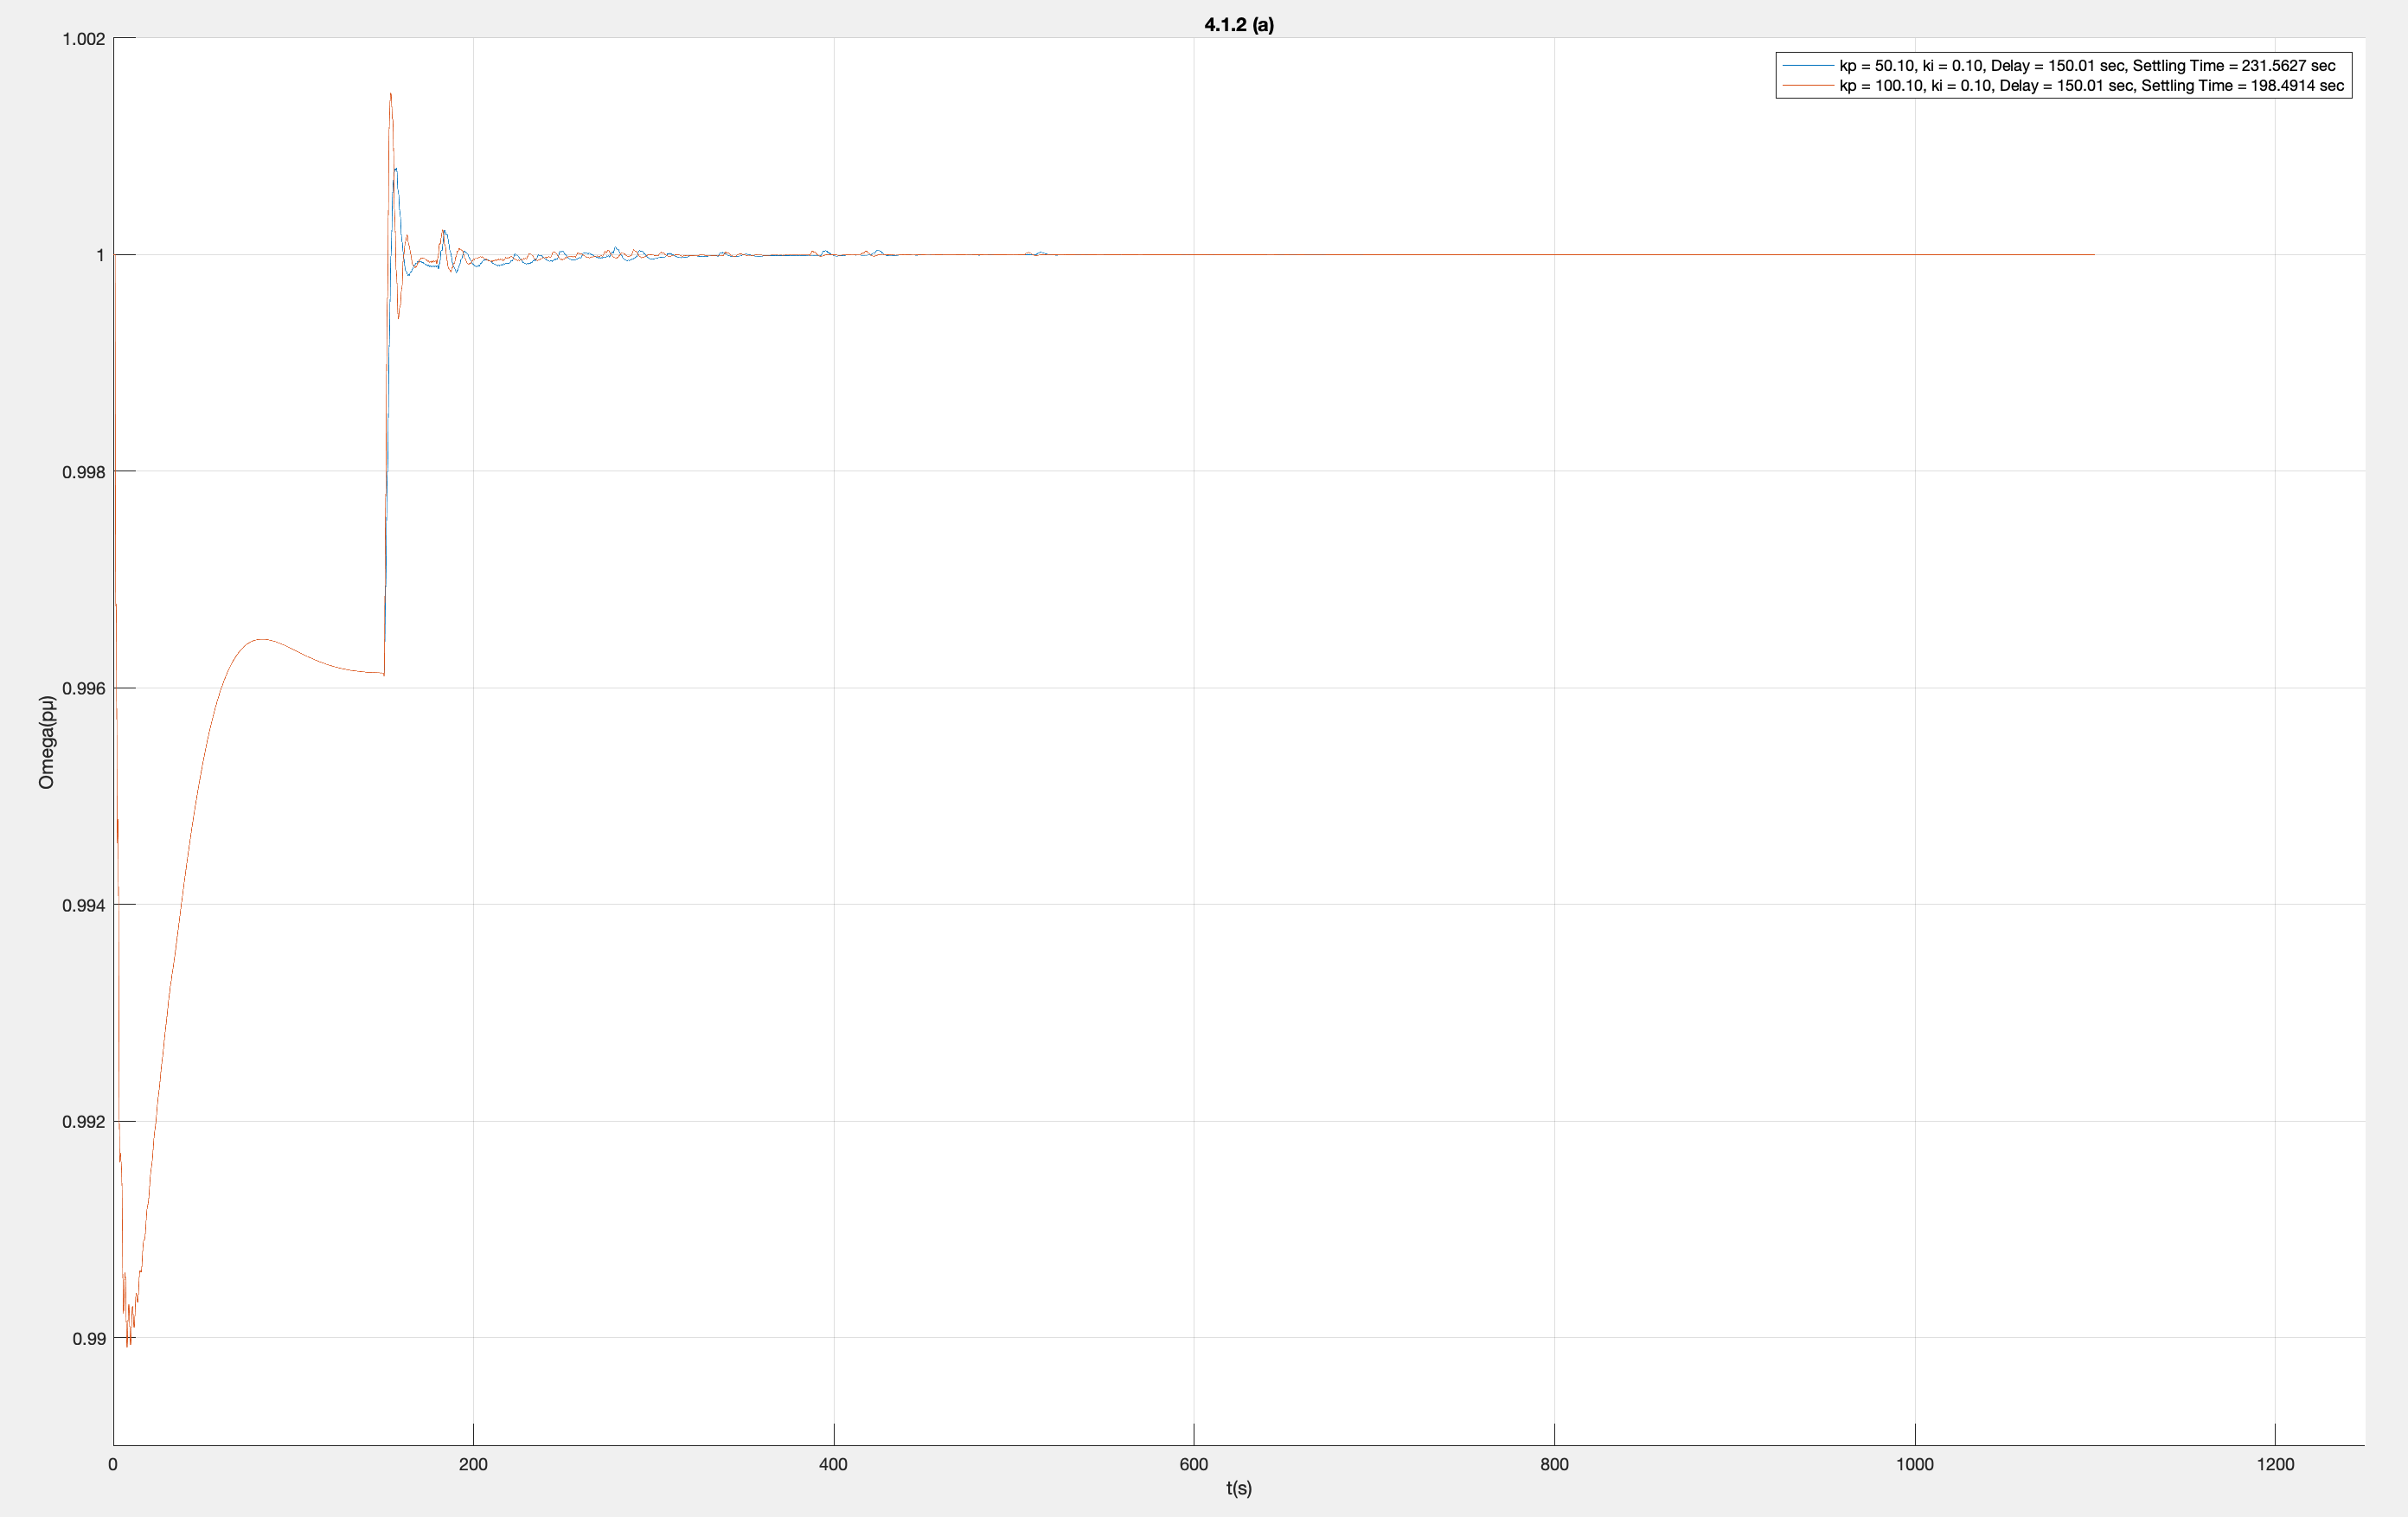
\includegraphics[width = .819\textwidth]{figure/4_1_2_a.png}
\caption{Disconnect generator g9: delay = 0.01, kp = 0.1~300.1, ki = 0.1~300.1, step: 50; start time (150s), end time (1100), settling time (1050s).}
\label{4_1_2_a}
\end{figure}

However, as you can see from Figure~\ref{4_1_2_a}, only two of all the simulations are acceptable. The maximum value of kp is 100.1 and the maximum value of ki is 0.1.  

According to the regulations from the last chapter, we need to increase the maximum amplifier factor by the step value.  

For instance, the new range of kp is between 0.1 and 150.1 and the new range of ki is between 0.1 and 50.1. To make more accurate results, we need to decrease the step at the same time. We set step be 10.0.  

Finally, we have another plot as shown in Figure~\ref{4_1_2_b}.  

\begin{figure}[htbp]
\centering
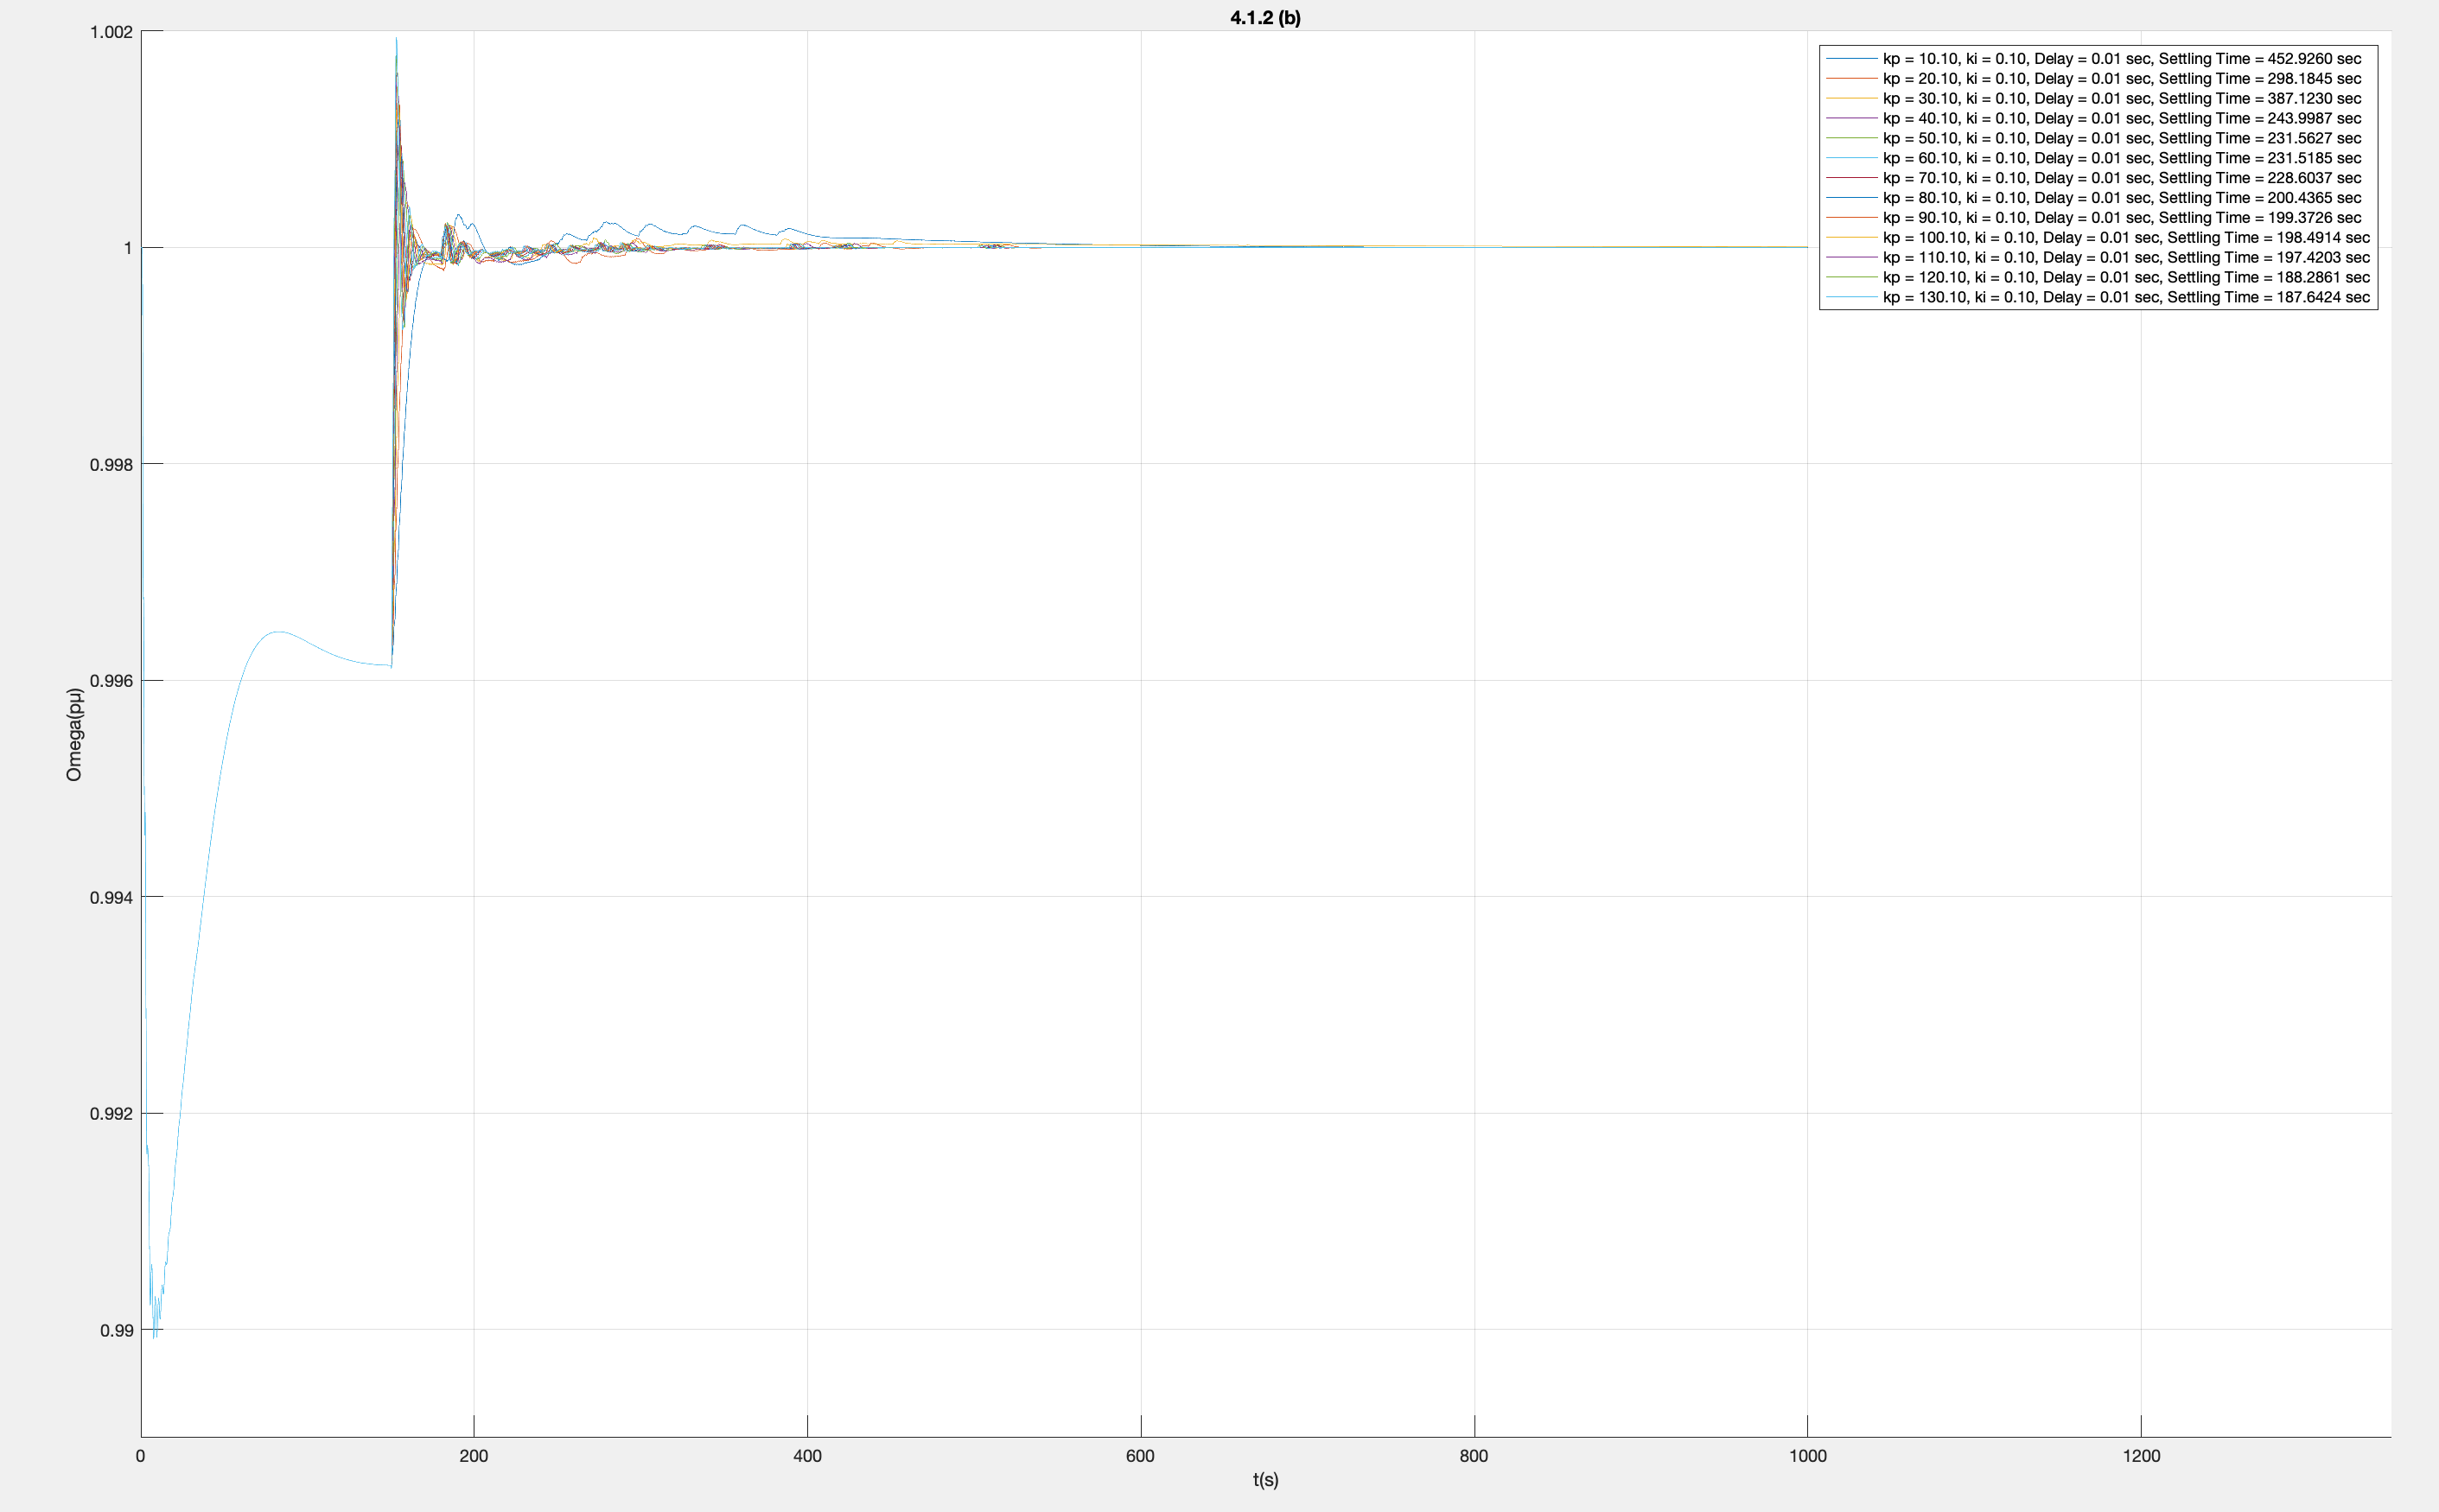
\includegraphics[width = .819\textwidth]{figure/4_1_2_b.png}
\caption{Disconnect generator g9: delay = 0.01, kp = 0.1~150.1, ki = 0.1~50.1, step: 10; start time (150s), end time (1100s), settling time (1050s).}
\label{4_1_2_b}
\end{figure}


Apparently, we have more acceptable results than last simulation because of shrinking the step of kp. We find that the simulations are unacceptable if kp equals to 140.1 or 150.1. Thus, we can finally fix the range of kp between 0.1 and 140.1 and keep the step of kp to 10.  

We could set ki in a range of 0.1 and 10.1 with the reason above. However, it is possible the maximum value of ki is still 0.1 if we set the range of ki be from 0.1 and 10.1. Then the simulations are meaningless.  

Thus, we need to apply bisection method again on the range of ki and find the meaningful maximum ki. Detailedly, we range kp from 0.1 to 140.1 and its step is 10.0. We set ki equals to 5.1. The purpose of doing this is to find if there are acceptable results if ki is in the middle of 0.1 and 10.1.    

The filtered results are as Figure~\ref{4_1_2_c}.  

\begin{figure}[htbp]
\centering
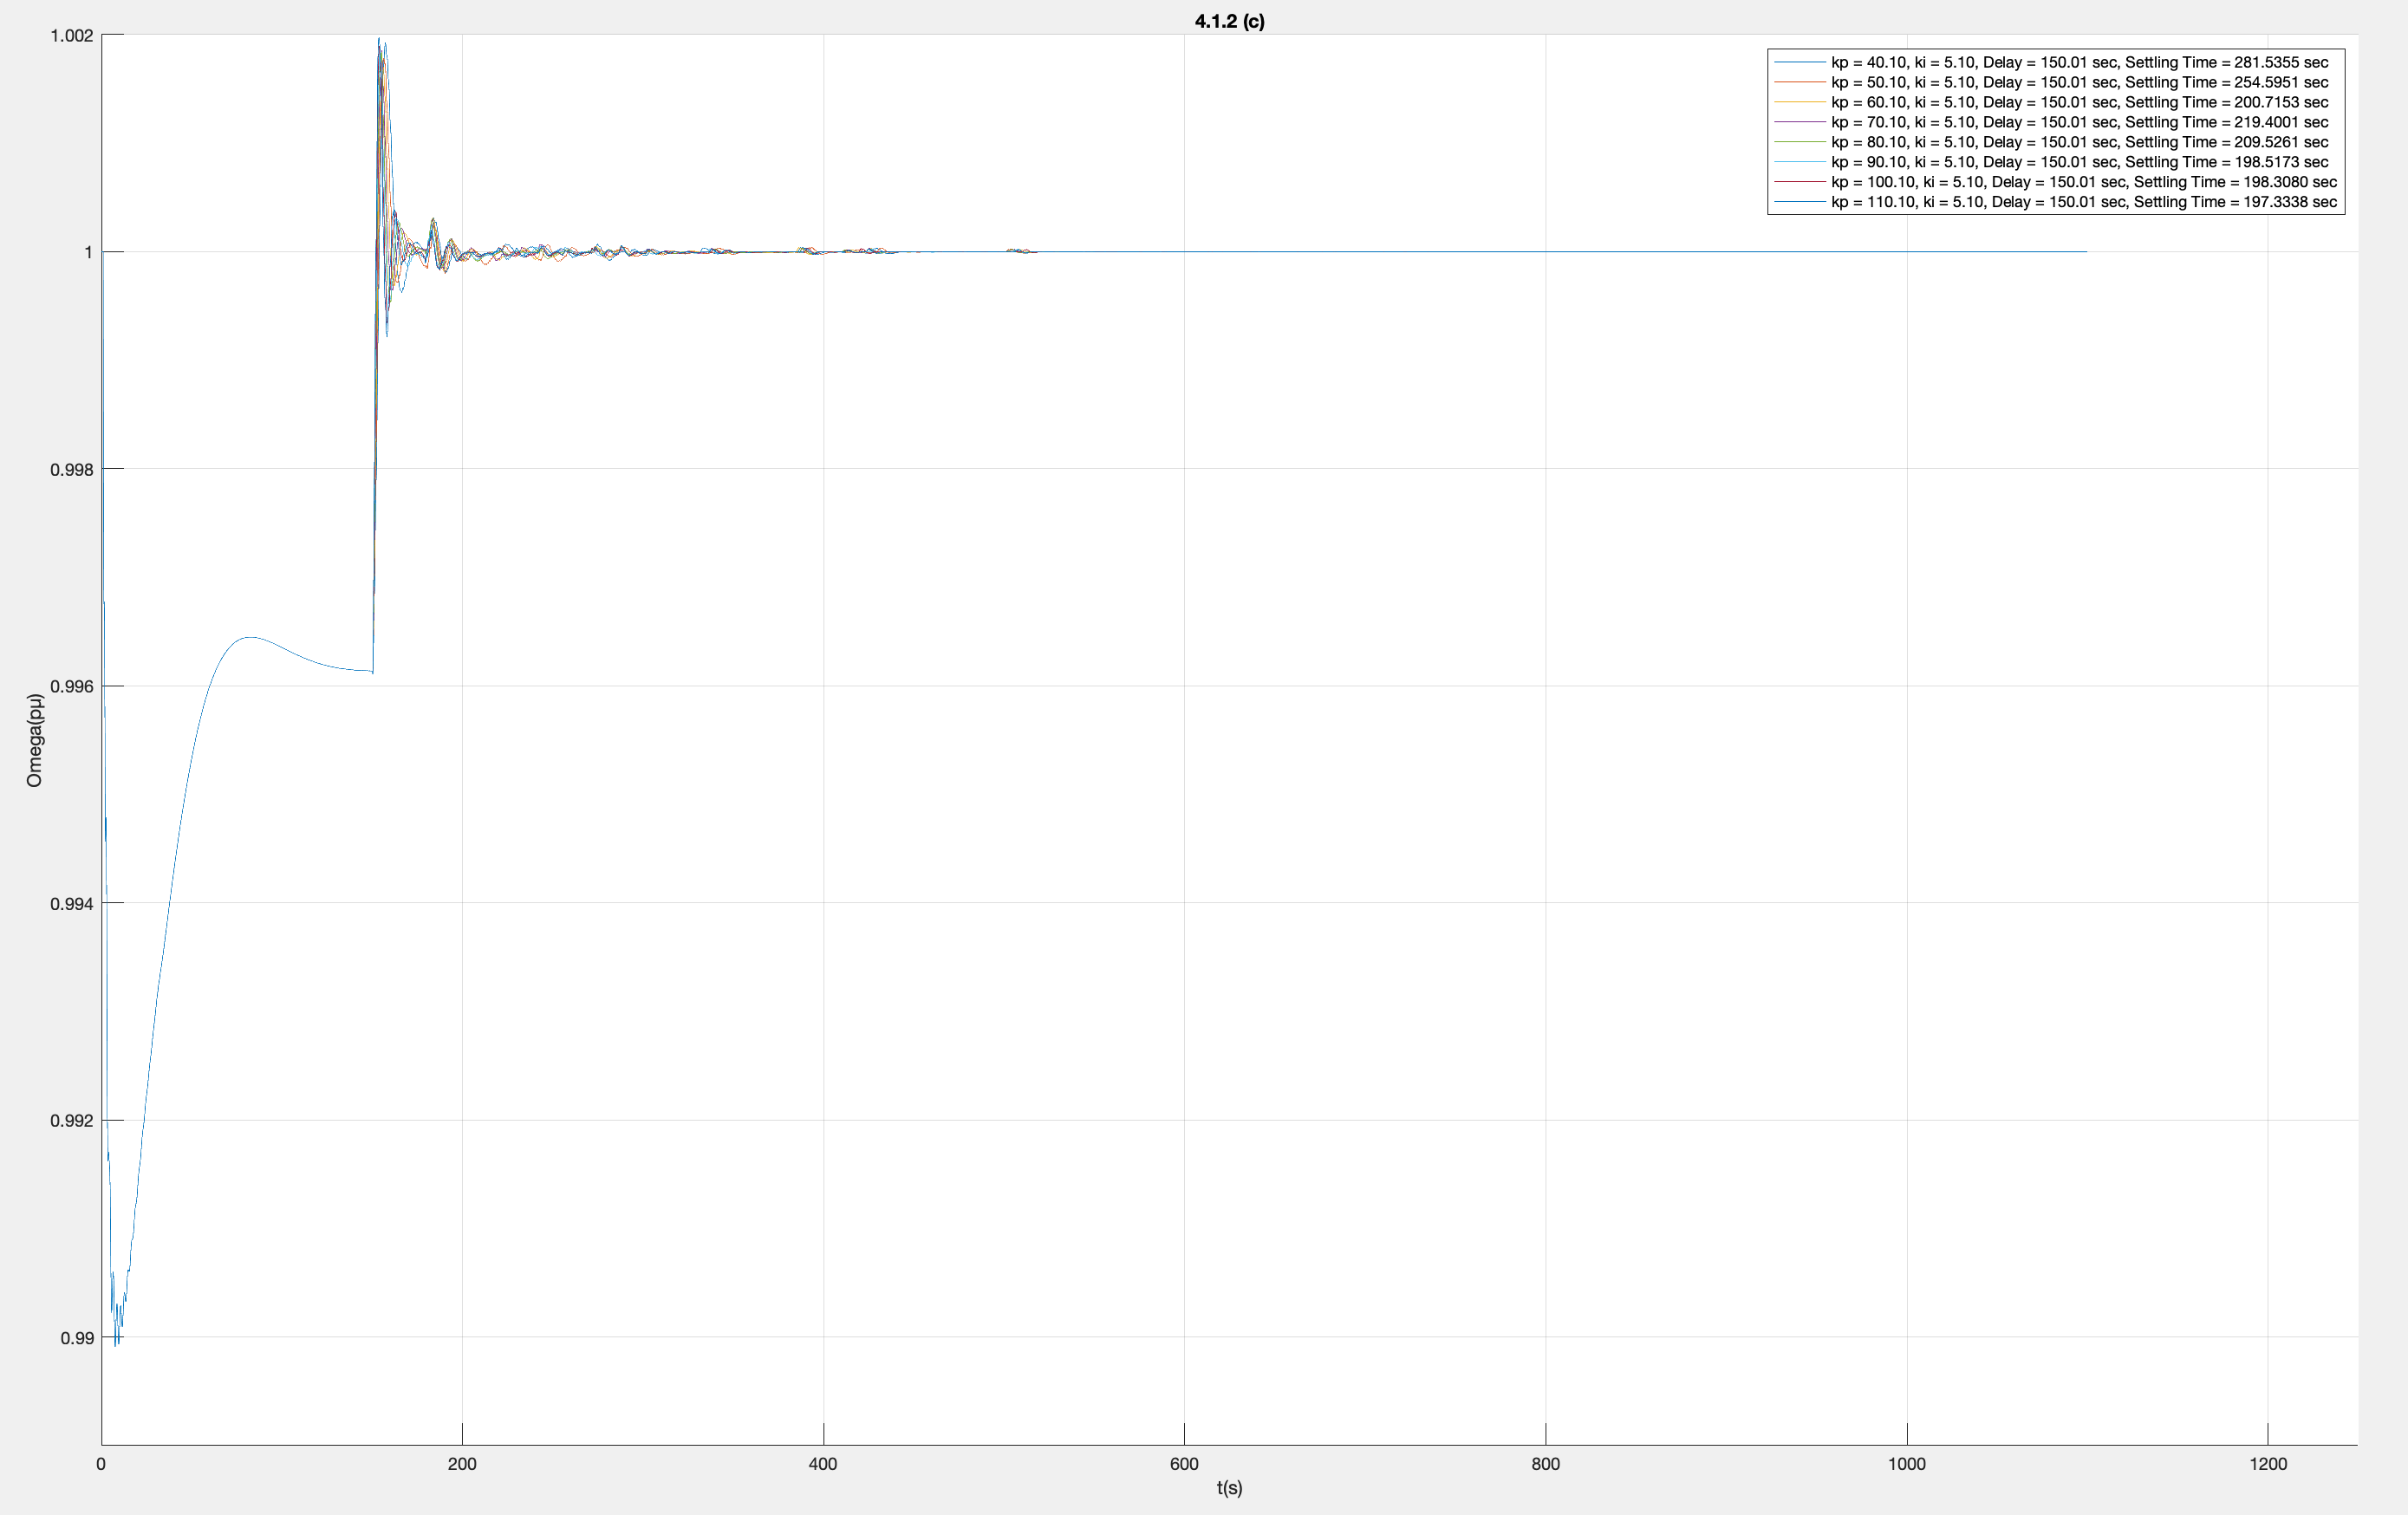
\includegraphics[width = .819\textwidth]{figure/4_1_2_c.png}
\caption{Disconnect generator g9: delay = 0.01, kp = 0.1~140.1, step: 10, ki = 5.1; start time (150s), end Time (1100s), settling time (1050s).}
\label{4_1_2_c}
\end{figure}

The results shows there are acceptable simulations if ki equals to 5.1.  

Thus, we can set the range of ki between 0.1 and 10.1. 
Besides, we can reset the end time to 240 seconds and the required settling time to 200 seconds since most of the acceptable simulations are settled before 200 seconds. 
\section{Expected Outcome} %4.2
\label{section4.2}

From discussions before, we know that both kp and ki can not be expanded indefinitely since we have specialised limit for kp and ki in MATLAB program. Thus, firstly, I hope to see a clear borderline that separates the acceptable and unacceptable results. The acceptable results will be expressed as blue points in Excel.  \\

Secondly, I hope to see a relationship between the best point, which has minimum settling time among all the acceptable results, and other acceptable points. I expect the best point will not appear in the borderline because the points in the borderline are likely to be unstable if the delay increases.  \\

I also do not hope the best point has a large or small kp and ki. A larger kp produce a larger overshoot although it would be relatively faster. A small kp has a larger probability of producing a steady-state error and it is relatively harder to approach a settled statement. A larger ki produces more oscillations, as Figure~\ref{3_4_1_larger_ki} shows, and thus it is also hard to approach a settled statement. A small ki does not help fixing the steady-state error along with a small kp.\\
\section{Implement} %4.3
One of the most important idea to implement the testing environment is to modularize the function. We modularize our functions, like the AGC algorithm, the moving file script and ending file script, in a python file so we can import them as a library and call them in the main file directly. Additionally, it is necessary to remove hard coded parameters so it is easy to change the parameters like start time, end time, prepared folder address and list of generators in the main function. 

Another noteworthy detail is we need to keep two significant digits for kp, ki and time delay. It provides an unified format that helps exporting data into analytical algorithms. 

\begin{figure}[htbp]
\centering
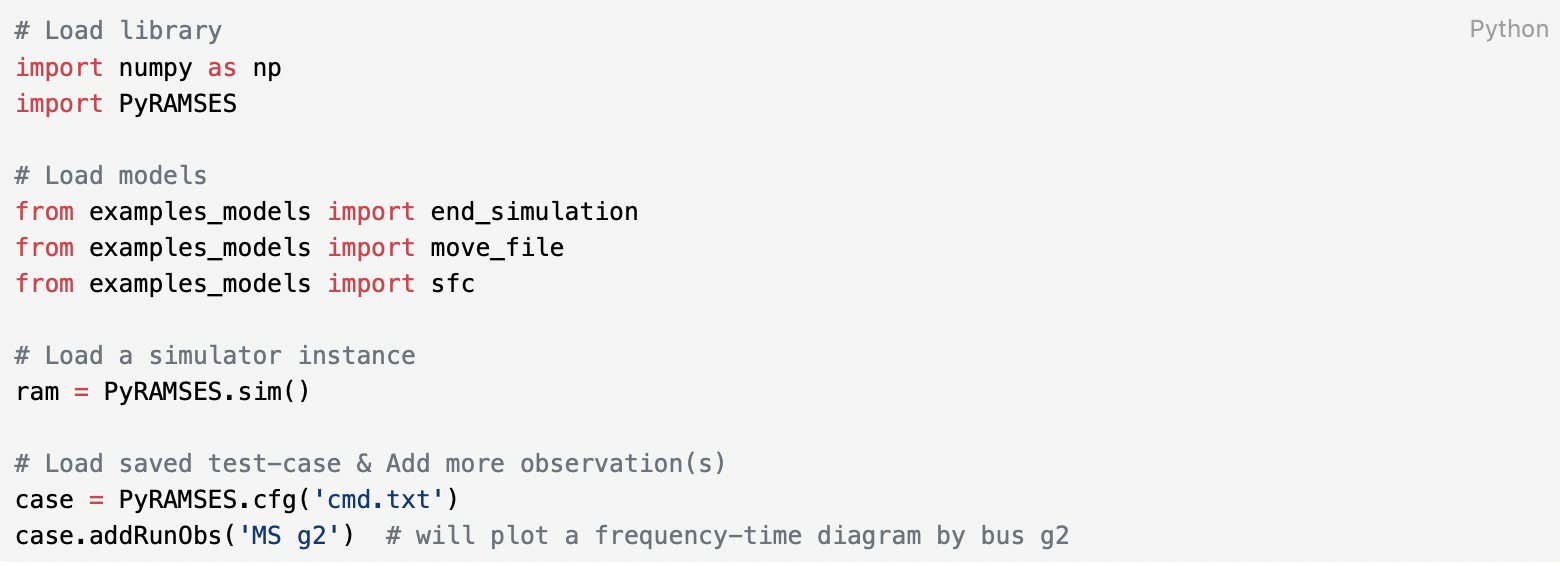
\includegraphics[width = \textwidth]{figure/4_3_code1.png}
\caption{Python: import related libraries.}
\label{4_3_code1}
\end{figure}

\begin{figure}[htbp]
\centering
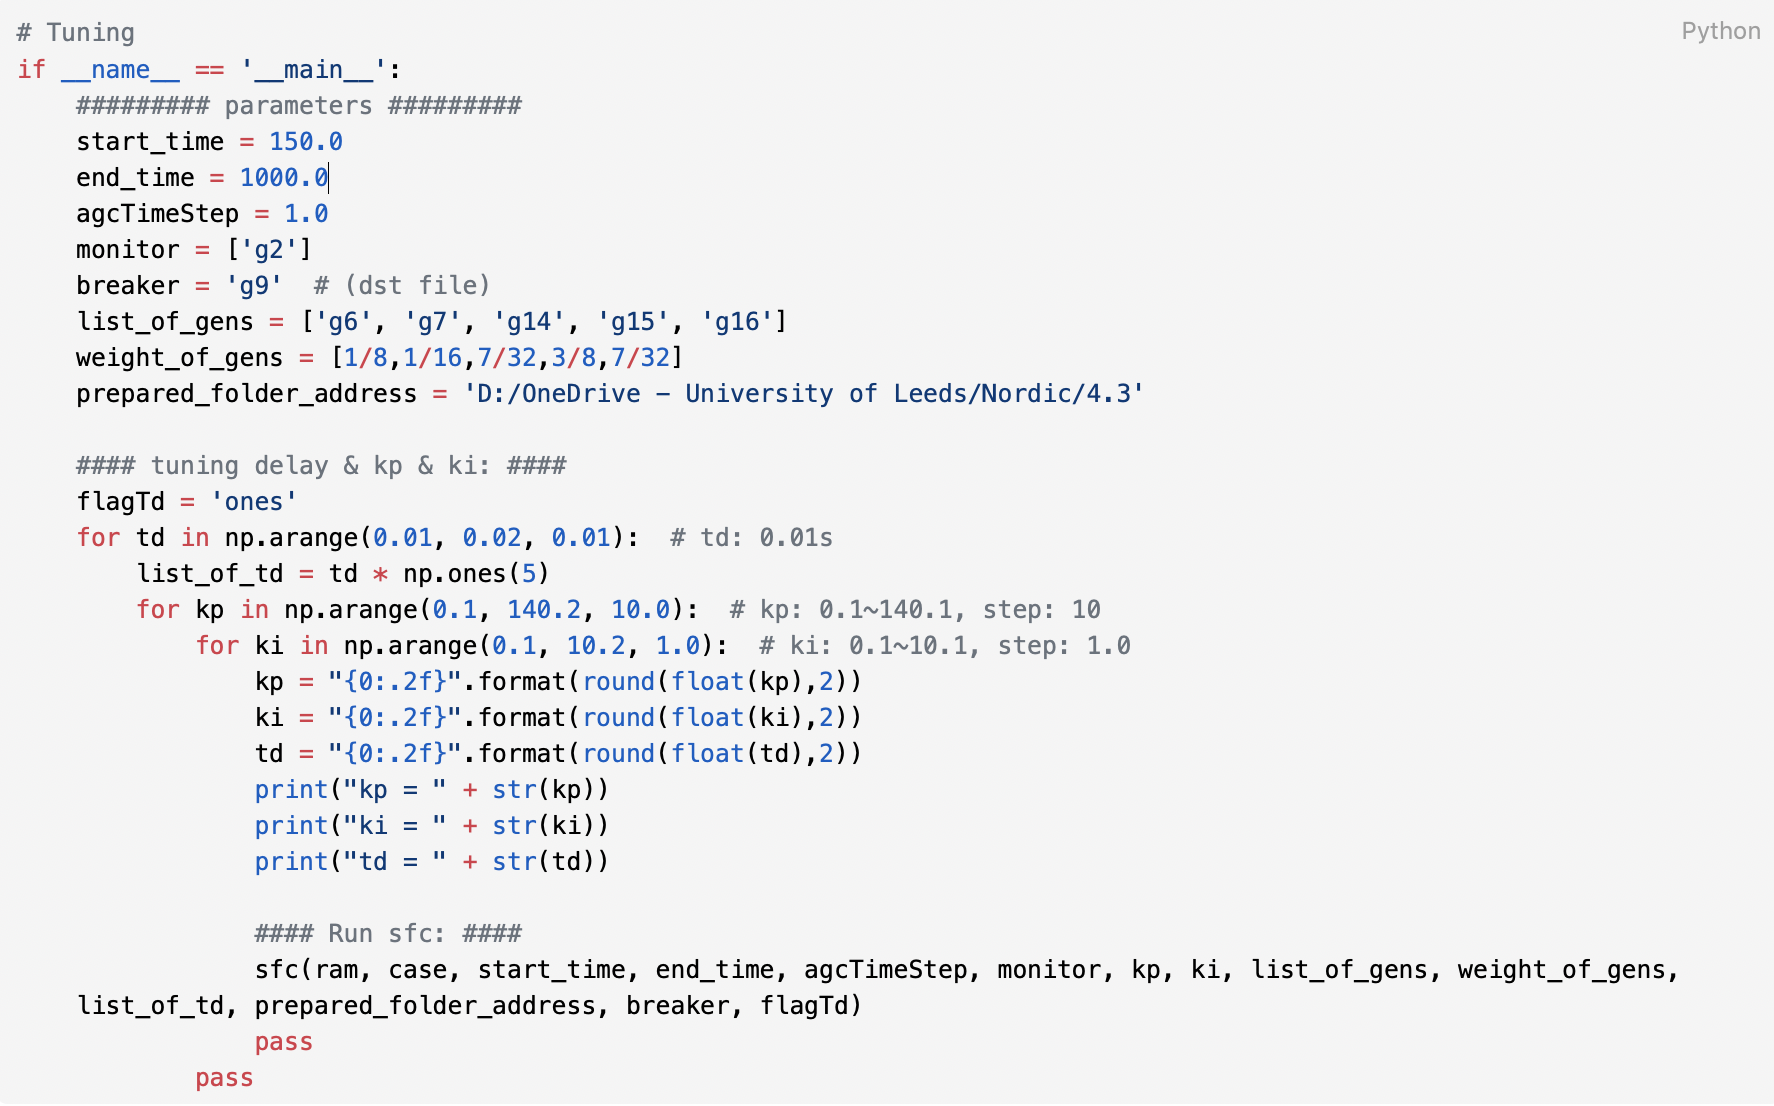
\includegraphics[width = \textwidth]{figure/4_3_code2.png}
\caption{Python: tune PI control.}
\label{4_3_code2}
\end{figure}
\section{Results} %4.4
\label{section4.4}
\subsection{Results and Analysis} %4.4.1
The implement results are as follows. Figure~\ref{4_4_1_result1} shows all the acceptable signals.

\begin{figure}[htbp]
\centering
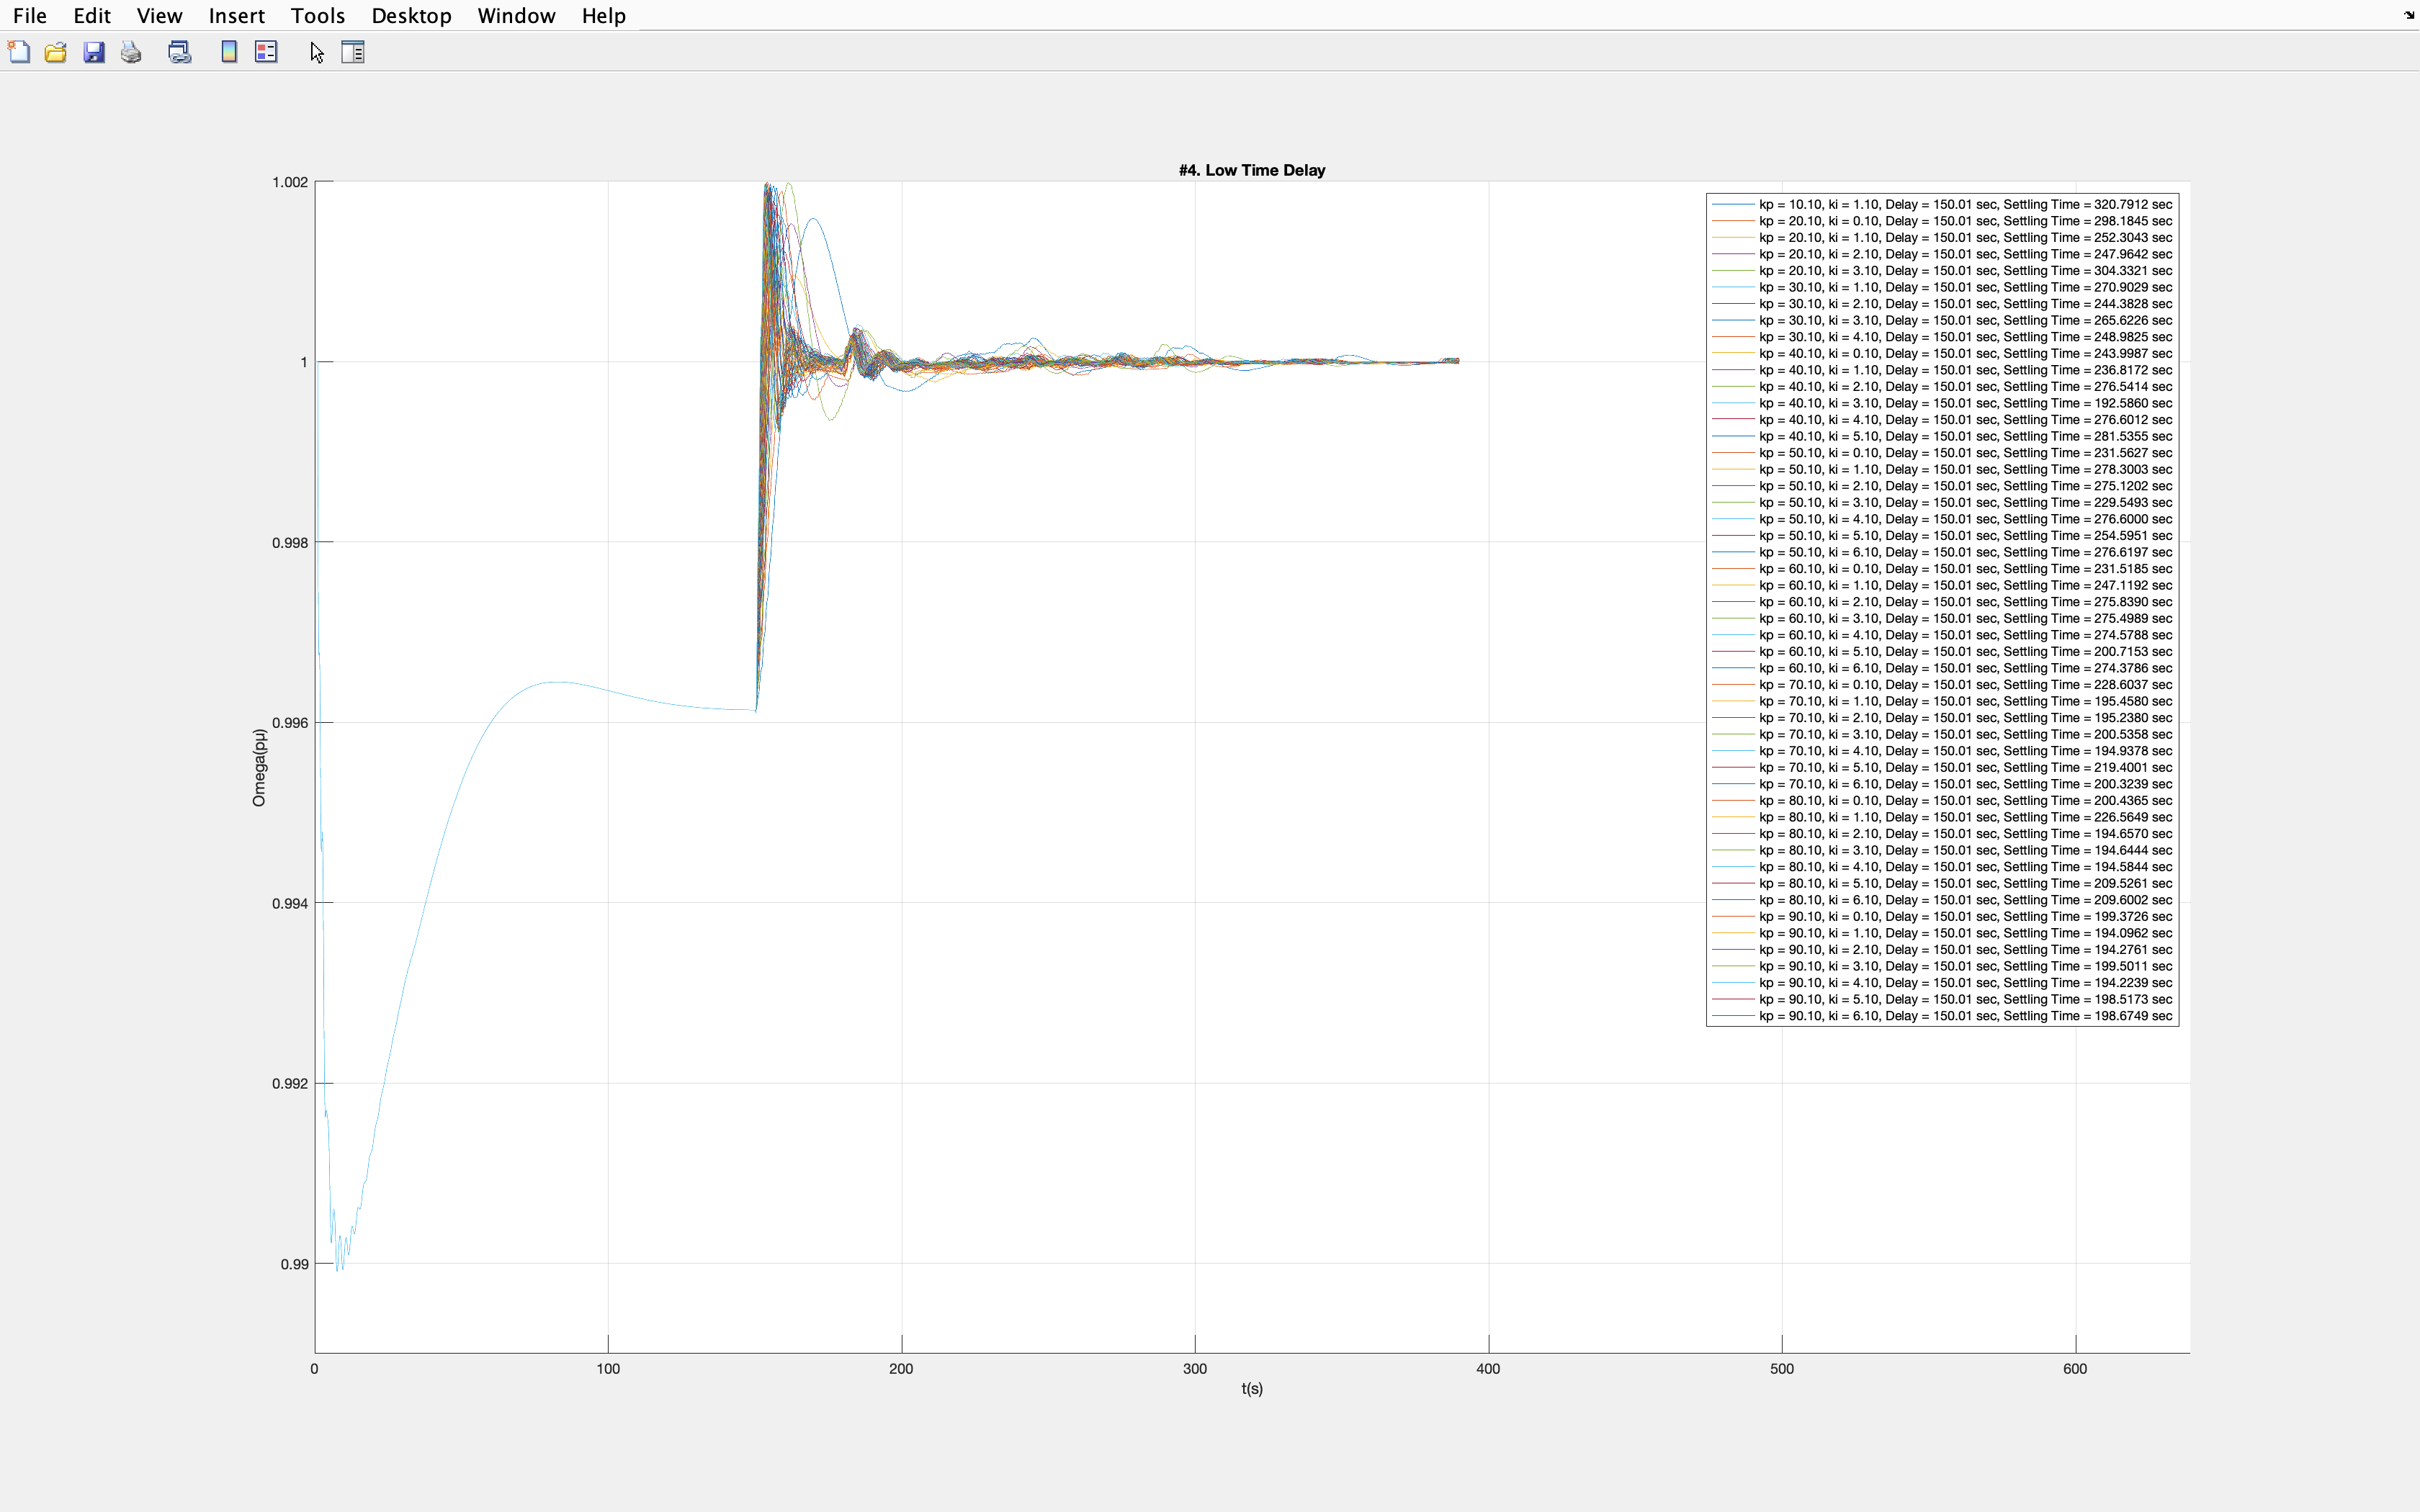
\includegraphics[width = .819\textwidth]{figure/4_4_1_result1.png}
\caption{MATLAB plot: all the acceptable signals.}
\label{4_4_1_result1}
\end{figure}

From Figure~\ref{4_4_1_result1}, we can roughly draw a conclusion that the signals are indeed within a reasonable range and it seems that they have finally reached the nominal value. \\

However, we need to check further by choosing one of the signals. For instance, I choose the signal whose kp is 90.1 and ki is 7.1. The reason I choose this signal is that it is located at the borderline. Results are as follows. \\

\begin{figure}[htbp]
\centering
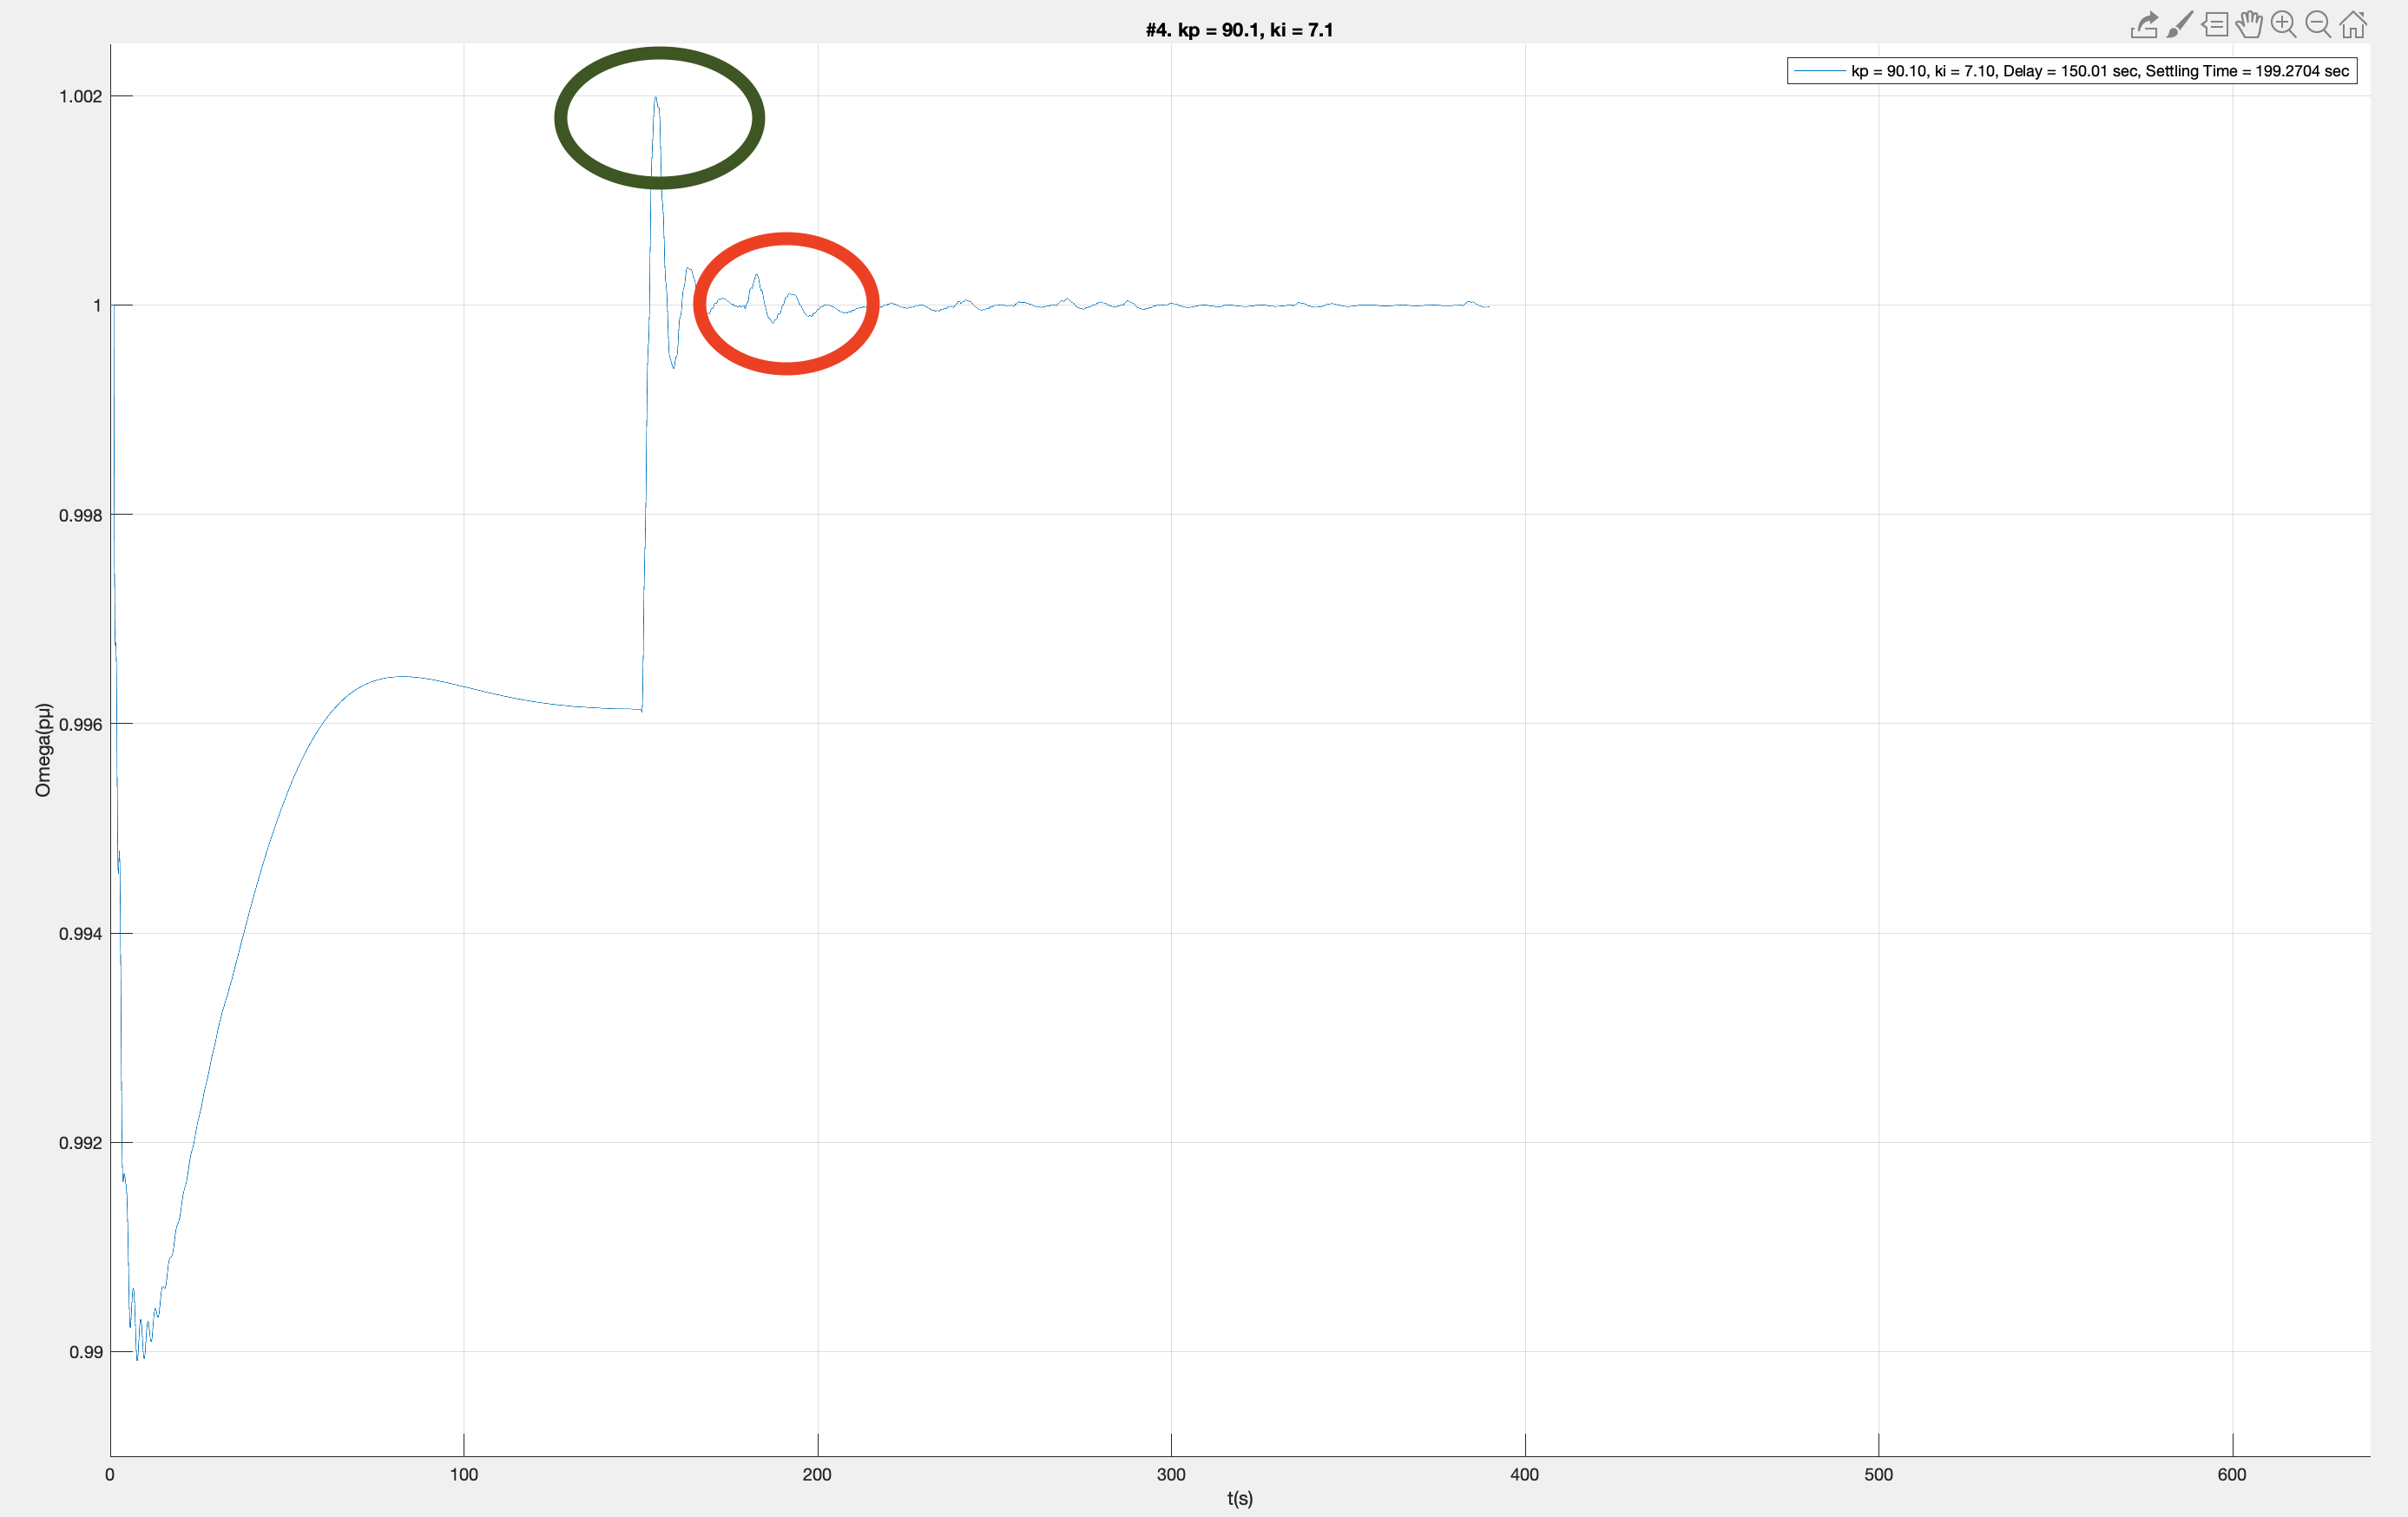
\includegraphics[width = .819\textwidth]{figure/4_4_1_result2.png}
\caption{The whole picture: whether the controlled signal meet the conditions: frequency limit and settling condition}
\label{4_4_1_result2}
\end{figure}

From the Figure~\ref{4_4_1_result2}, we can see that the overshoot does not exceed 1.002 obviously. But for the settling time, we can not make any conclusion until we see the details. \\


\begin{figure}[htbp]
\centering
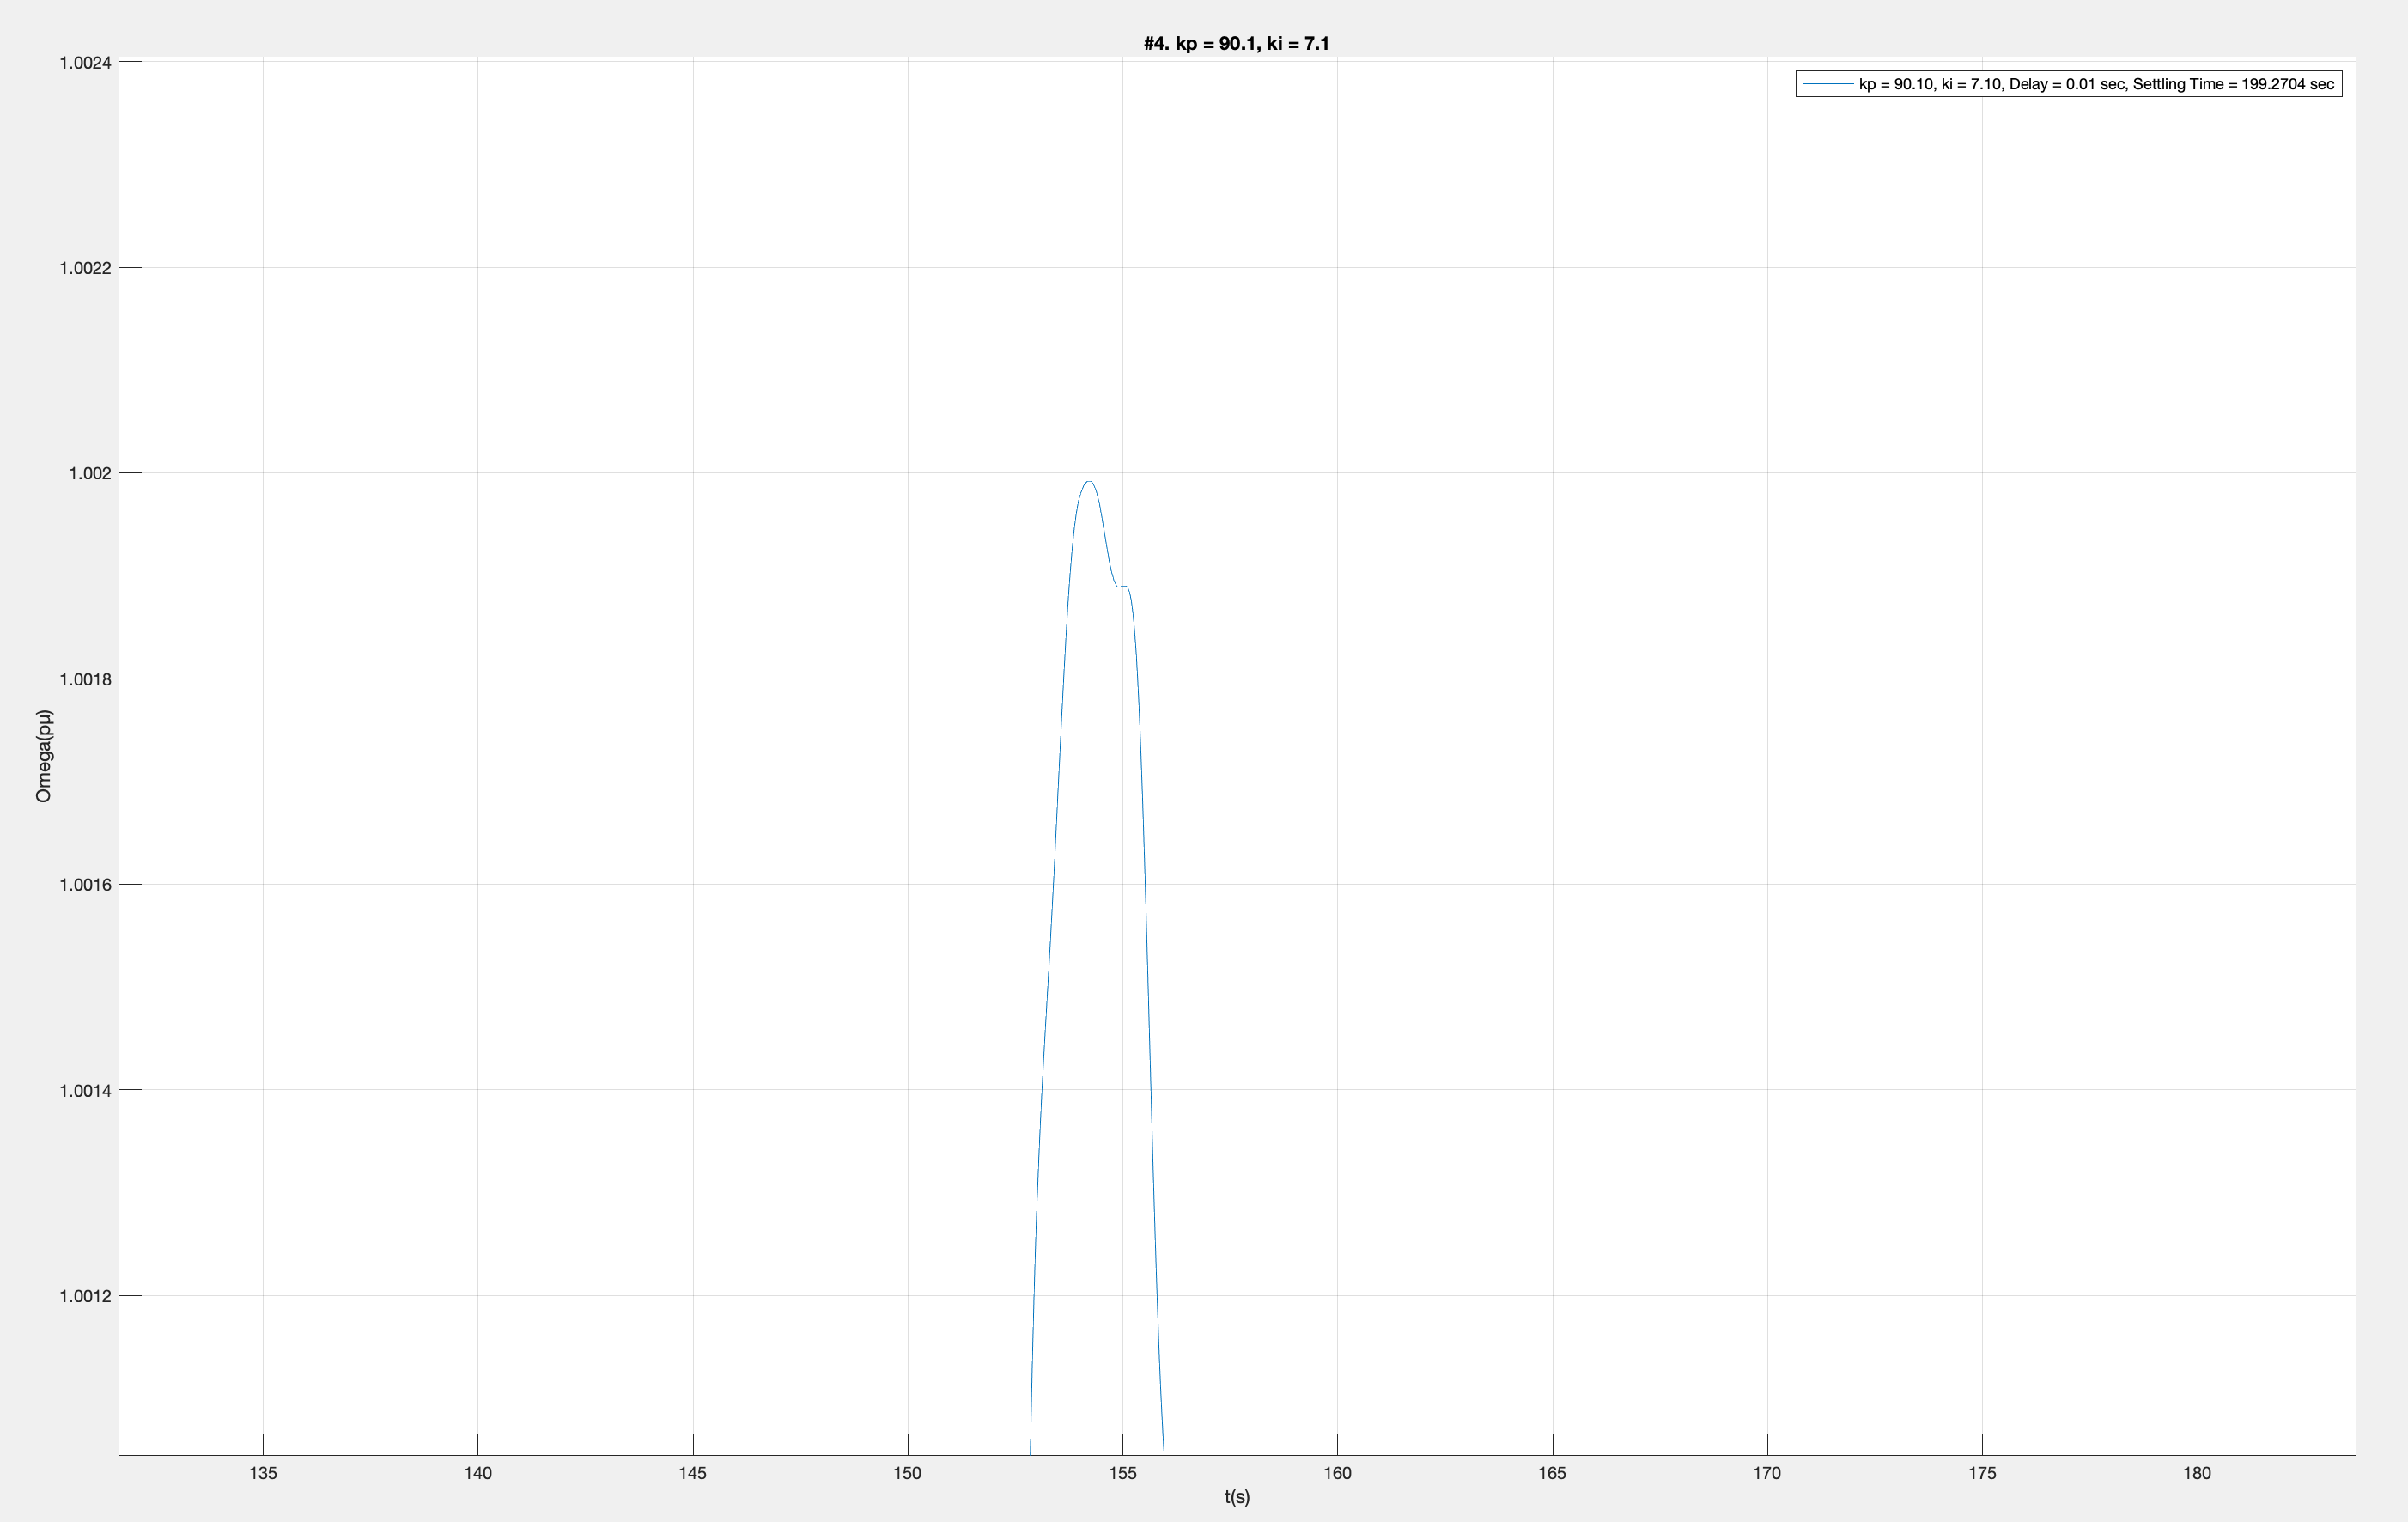
\includegraphics[width = .819\textwidth]{figure/4_4_1_result3.png}
\caption{Details: check frequency limit.}
\label{4_4_1_result3}
\end{figure}

From Figure~\ref{4_4_1_result3}, we can judge that its overshoot does not exceed the maximum allowable value, i.e. 1.002 $p\mu$, after the signal settled.\\

\begin{figure}[htbp]
\centering
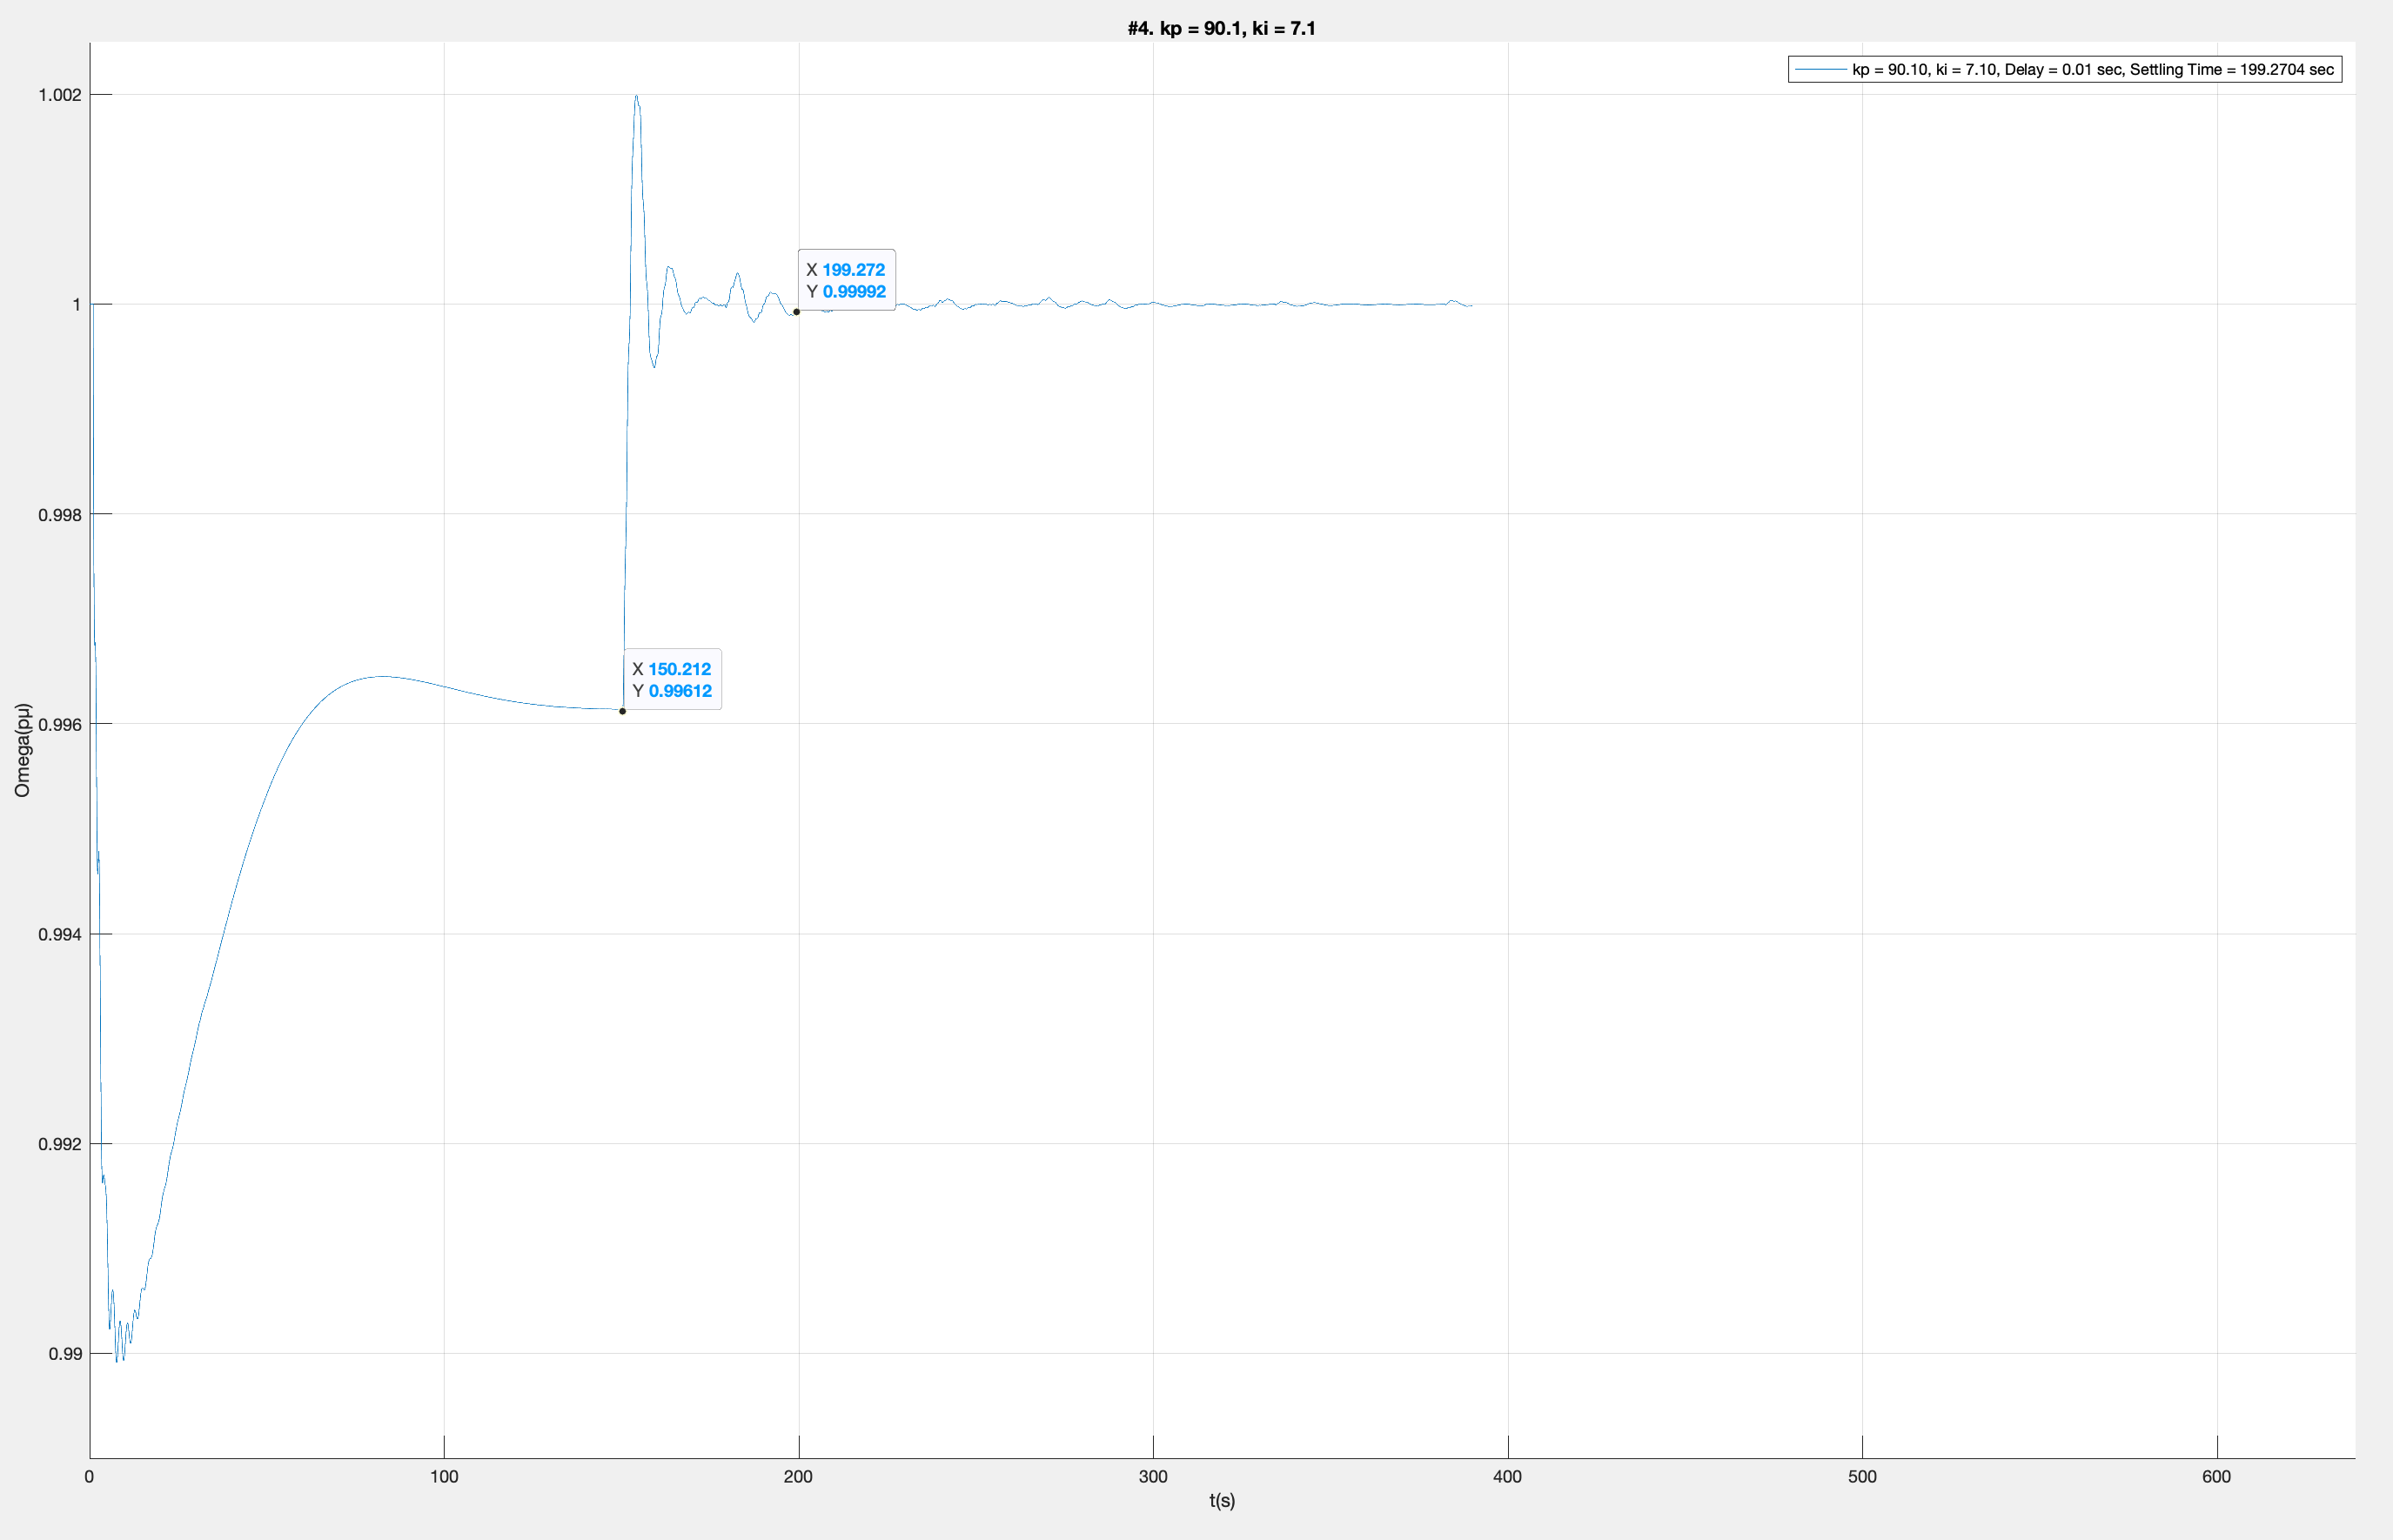
\includegraphics[width = .819\textwidth]{figure/4_4_1_result4.png}
\caption{Details: check settling condition.}
\label{4_4_1_result4}
\end{figure}


From Figure~\ref{4_4_1_result4}, we find that, after the signal settled, the signal is between the settling time threshold, i.e. 0.9998 $p\mu$ and 1.0002 $p\mu$.\\


With the prove above, we can finally say that our assumed acceptable simulation results are acceptable.\\

Next, we show you the relationship between kp and ki.\\

\begin{table*}[htbp]
\centering
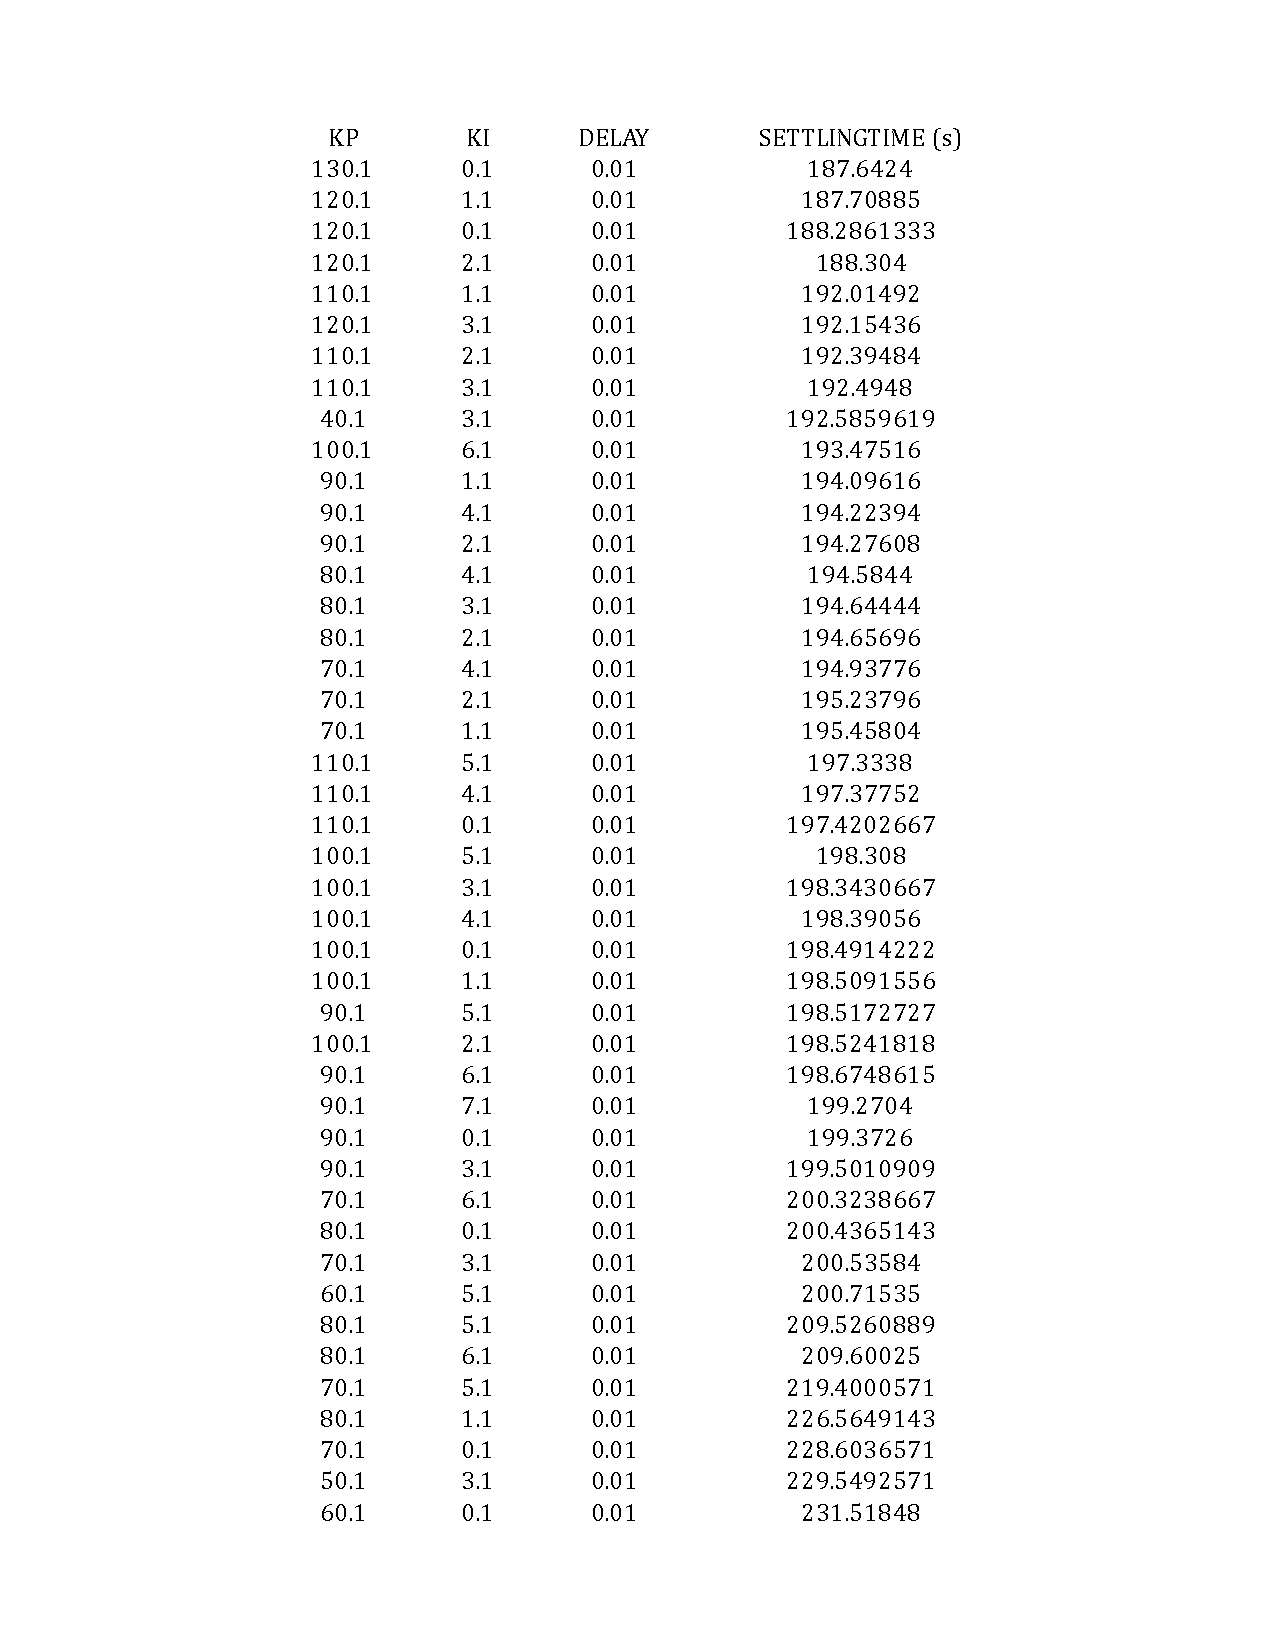
\includegraphics[width = \textwidth]{figure/4_4_1_table.pdf}
\caption{Part of the acceptable results ranked by settling time.}
\label{4_4_1_table}
\end{table*}

 Table~\ref{4_4_1_table} shows the parameters that make up the acceptable signals, i.e. kp, ki, delay and settling time. It has ranked by the settling time. \\

\begin{figure}[htbp]
\centering
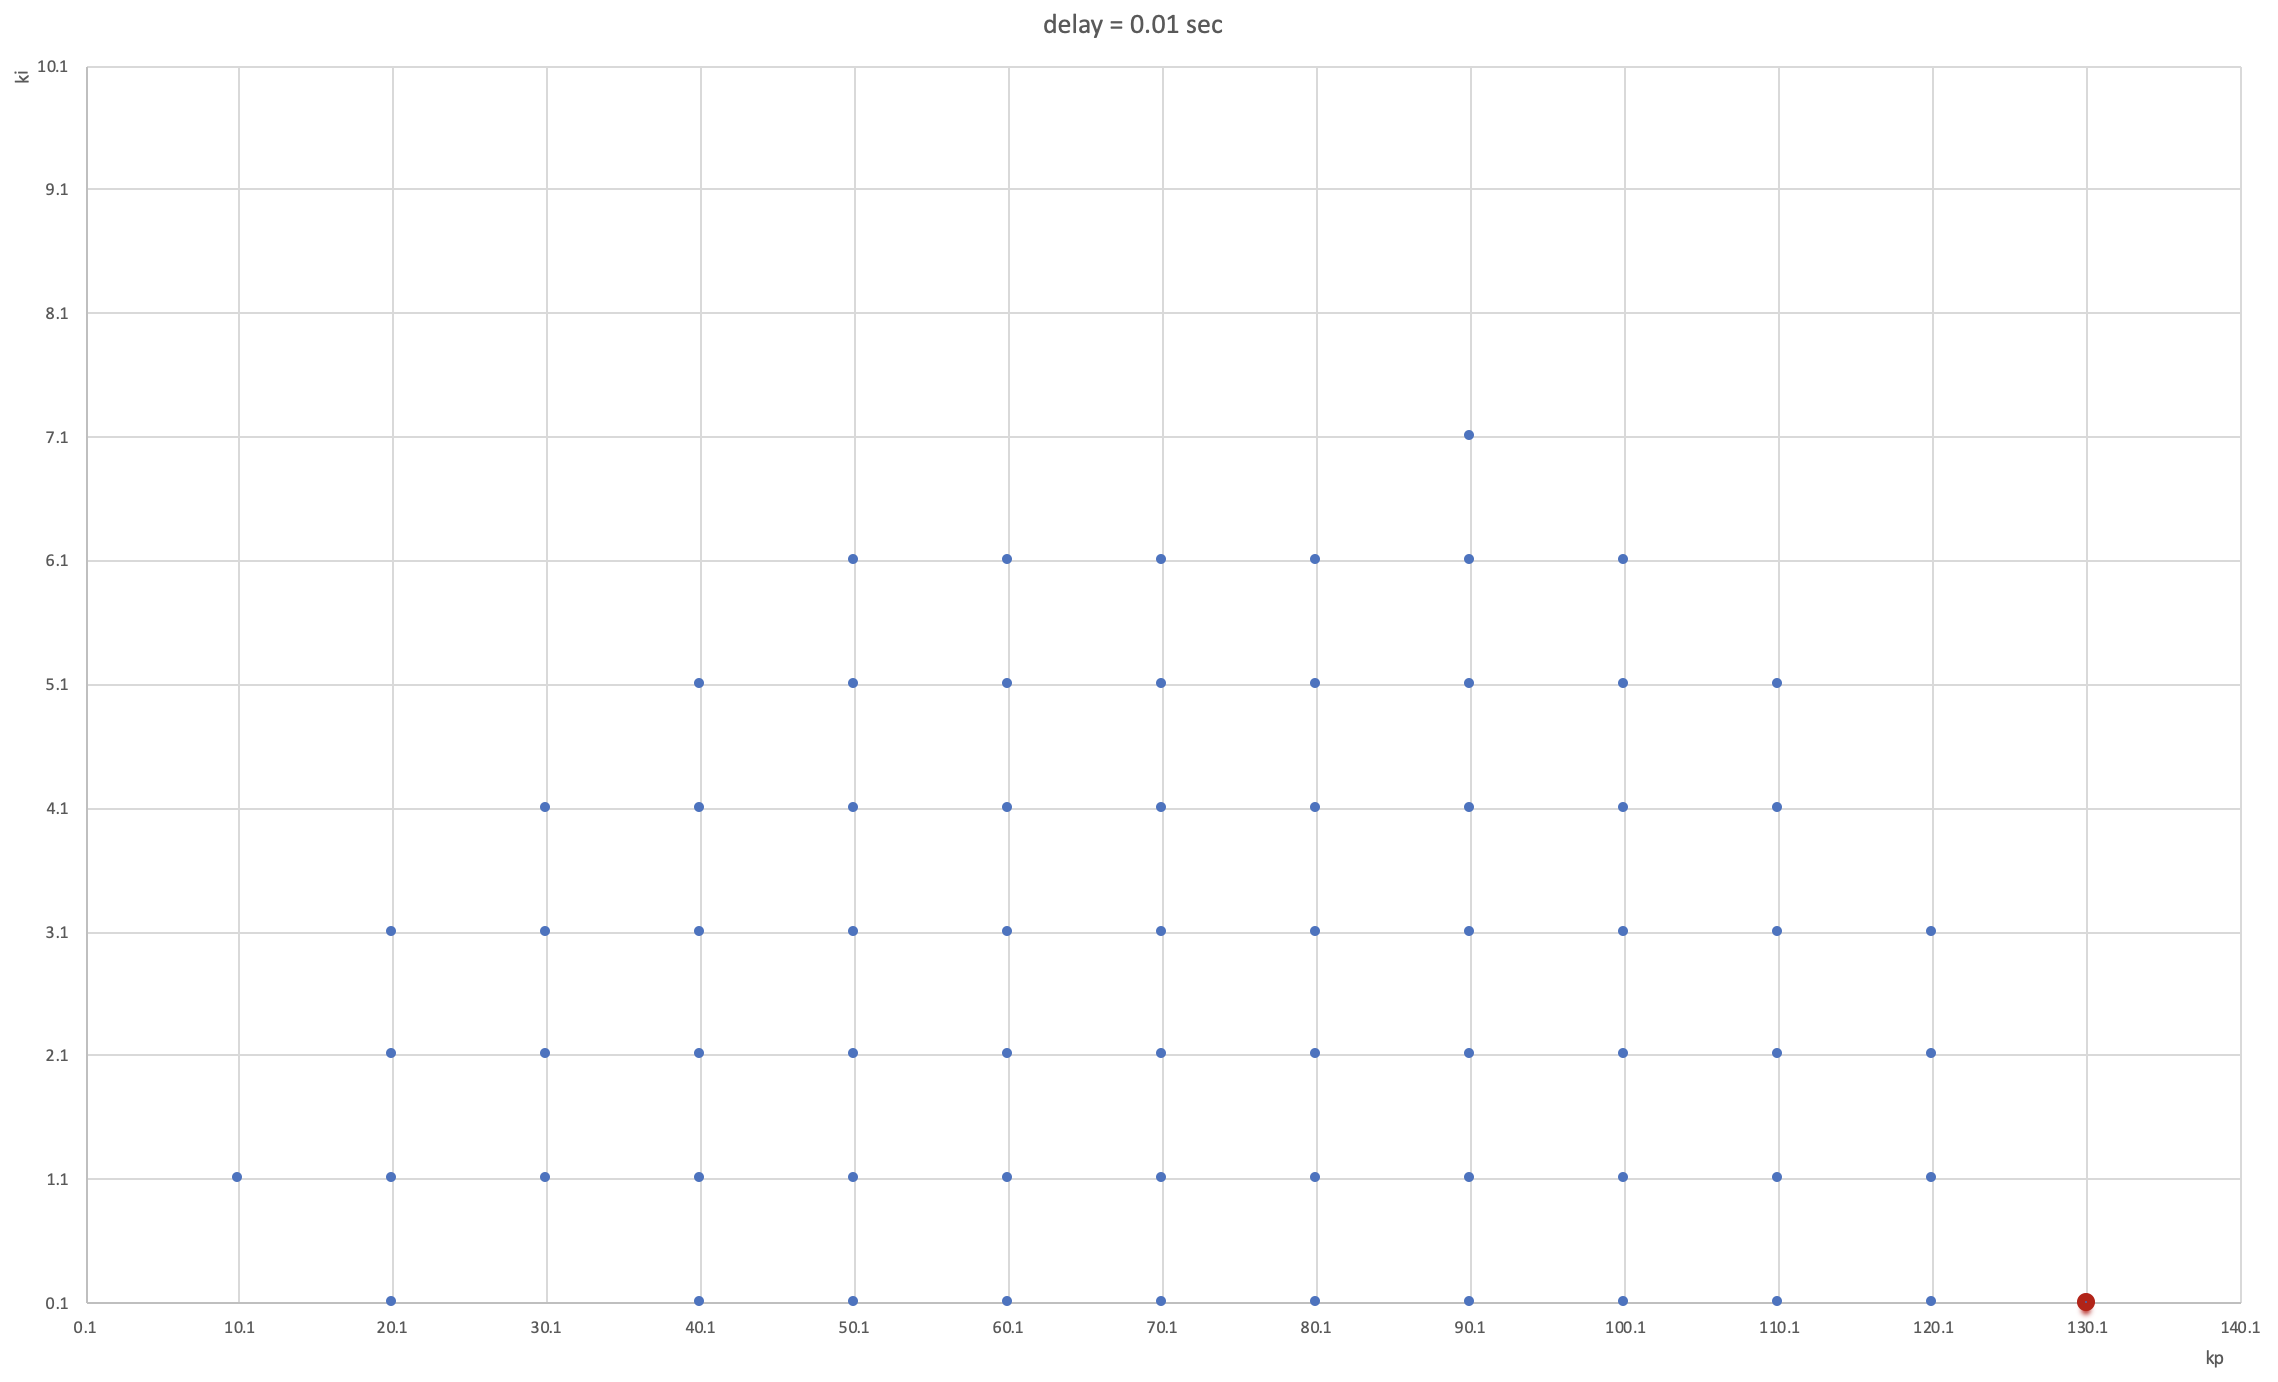
\includegraphics[width = .819\textwidth]{figure/4_4_1_2d.png}
\caption{2D plot: All the acceptable tuning results in low time delay.}
\label{4_4_1_2d}
\end{figure}

Table~\ref{4_4_1_2d} draws a 2D graph where kp is horizontal axis and ki is vertical axis. Besides, we highlight the point which gives the minimum settling time as a reference.\\

Analysing the Table~\ref{4_4_1_2d}, we can find:\\

\begin{itemize}
\item The 2D graph shows a clear borderline which separates the acceptable results and unacceptable results. This is in line with the previous expectation from section~\ref{section4.2};\\

\item The best point is (130.1, 0.1);\\

\item The best point is in the borderline.  This is not in line with the previous expectation from section~\ref{section4.2};\\

\item The best point’s kp value is too large. This is not in line with the previous expectation from section~\ref{section4.2};\\

\item The best point's ki value is not too large.  This is in line with the previous expectation from section~\ref{section4.2};\\

\item The worst point, i.e. kp is 10.1 and ki is 1.1, shows in the borderline. This is in line with the previous expectation from section~\ref{section4.2}.\\
\end{itemize}

Although, for the best point, its kp is large enough to keep the signal approaching the settling status as fast as possible, it is dangerous that it would be removed by a higher time delay.\\

However, the best point's ki value is 0.1, which is “unexpected” before. \\

There are two explanations for this small ki value. The first explanation is that this “small” ki value is not small enough or is not the smallest because it is assumed that 0.1 is the minimum value of the range of ki at the beginning of the simulation. We do not need to find the real limit value of ki in this case because it will increase the amount of computation by an order of magnitude. There might be acceptable results whose kp is smaller than 0.1 but it is not necessary to find them in this case. \\

Another explanation is that the function of the I-term is to help fixing the steady-state error. In fact, steady-state error will not be always shown if only there is a suitable kp being tuned. Besides, a larger ki will produce more oscillations and it makes a longer settling time. \\


\subsection{The Best Tuning Signal} %4.4.2

\begin{figure}[htbp]
\centering
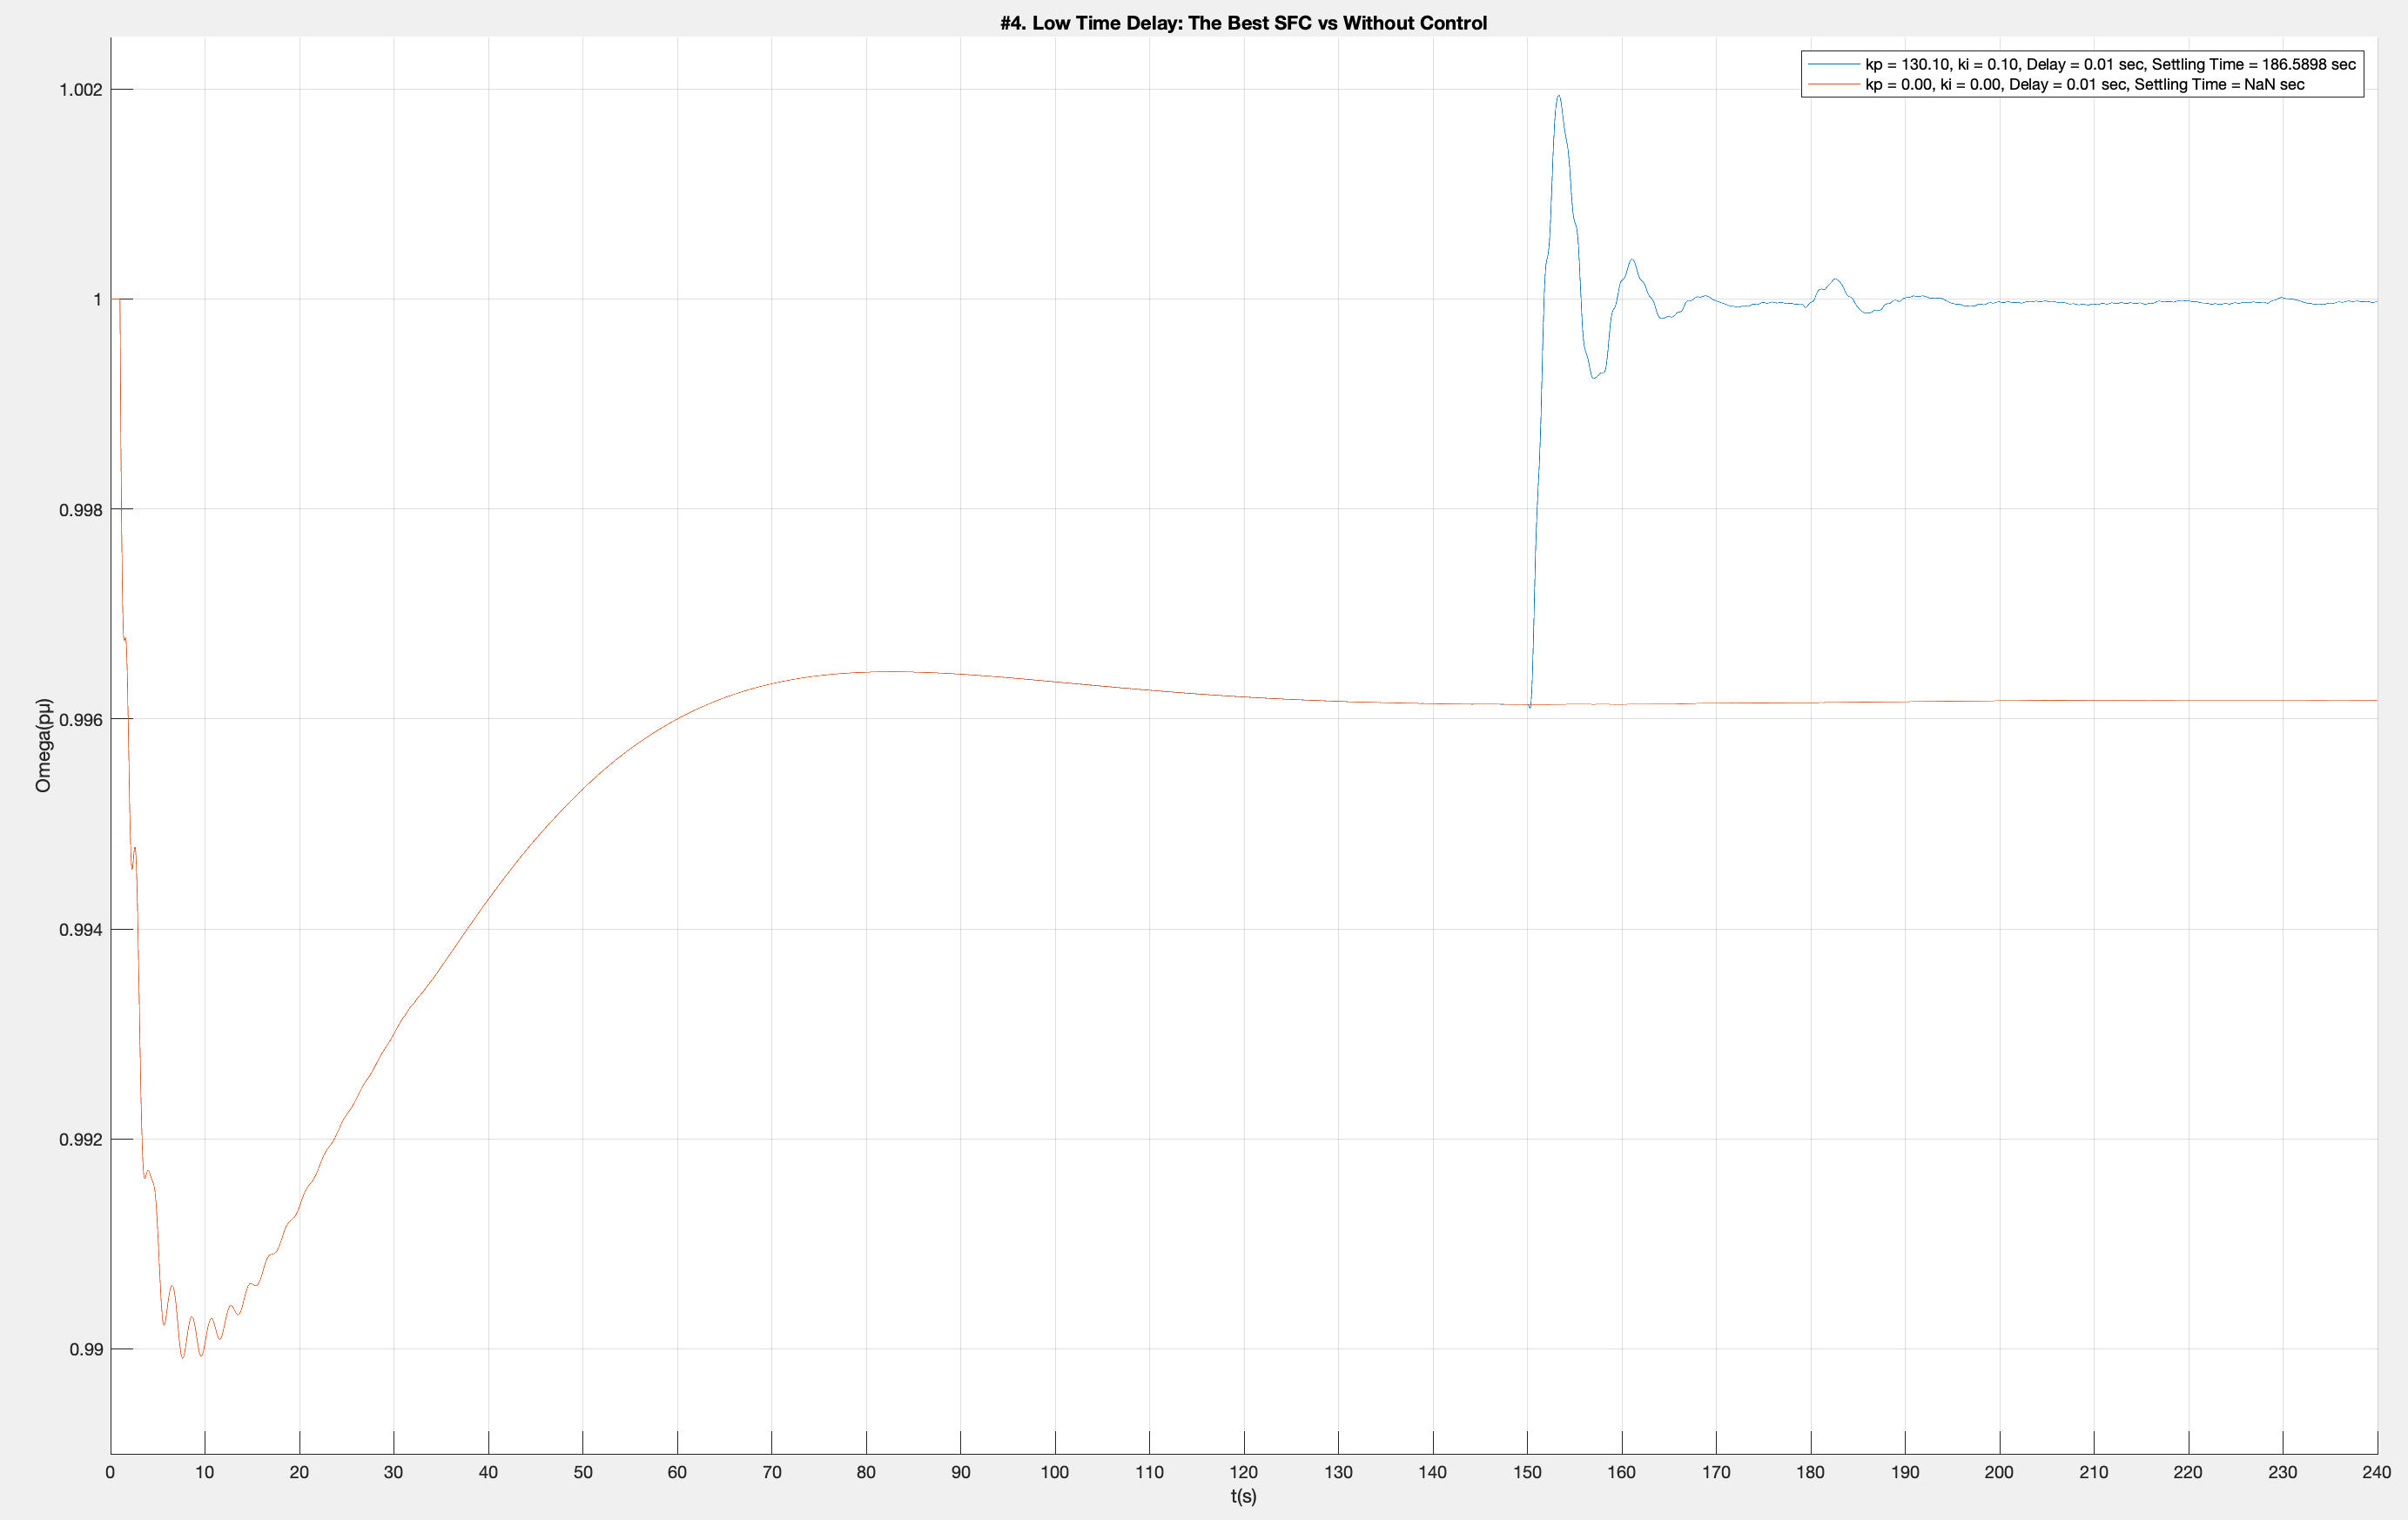
\includegraphics[width = .819\textwidth]{figure/4_4_2_best.png}
\caption{The best tuning signal}
\label{4_4_2_best}
\end{figure}
\section{Ramp Rate Analysis} %4.5
\label{section4.5}

From Section~\ref{section3.5}, we understand the importance of using ramp rate in power system. The aim is to be realistic. This is a real constraint in physical systems. The control cannot be used in reality if do not set the limit of it.\\

In Section~\ref{section3.5}, we discussed the reason to use \sys{peak} and \sys{peaktime} to calculate the ramp rate. Equation is as follow.

\begin{equation}
    Rate = \frac{P_{\sys{peak}} - P_o}{\sys{PeakTime}}
\end{equation}


Next, we can calculate the limit of ramp rate of generators. According to National Renewable Energy Lab., Golden, CO (US), \cite{osti_15016292} large thermal units are usually able to ramp around 1\% of their capacity per minute. Thus, we have Table~\ref{4_5_nominal_rate}:


\begin{table}[htbp]
  \centering
    \begin{tabular}{ccccc}
    Generator & Pnom~\footnote{Pnom (nominal power) is original from:~\href{https://github.com/realgjl/sfcNordic/blob/master/examples/dyn\_A.dat}{https://github.com/realgjl/sfcNordic/blob/master/examples/dyn\_A.dat}} (MW) & Ramp Rate (MW/min) & Ramp Rate (MW/sec)\\
    g6    & 360   & 3.6   & 0.06\\
    g7    & 180   & 1.8   & 0.03\\
    g14   & 630   & 6.3   & 0.105\\
    g15   & 1080  & 10.8  & 0.18\\
    g16   & 630   & 6.3   & 0.105\\
    \end{tabular}
  \caption{Nominal ramp rate of generators}
  \label{4_5_nominal_rate}
\end{table}

Then we can use the limit of ramp rate from Table~\ref{4_5_nominal_rate} to remove some tuning results. The source code~\footnote{See \href{https://github.com/realgjl/sfcNordic/blob/master/analysis/4.5/risk\_lowTd.m}{https://github.com/realgjl/sfcNordic/blob/master/analysis/4.5/risk\_lowTd.m}} is open to public. \\

\begin{table*}[htbp]
\centering
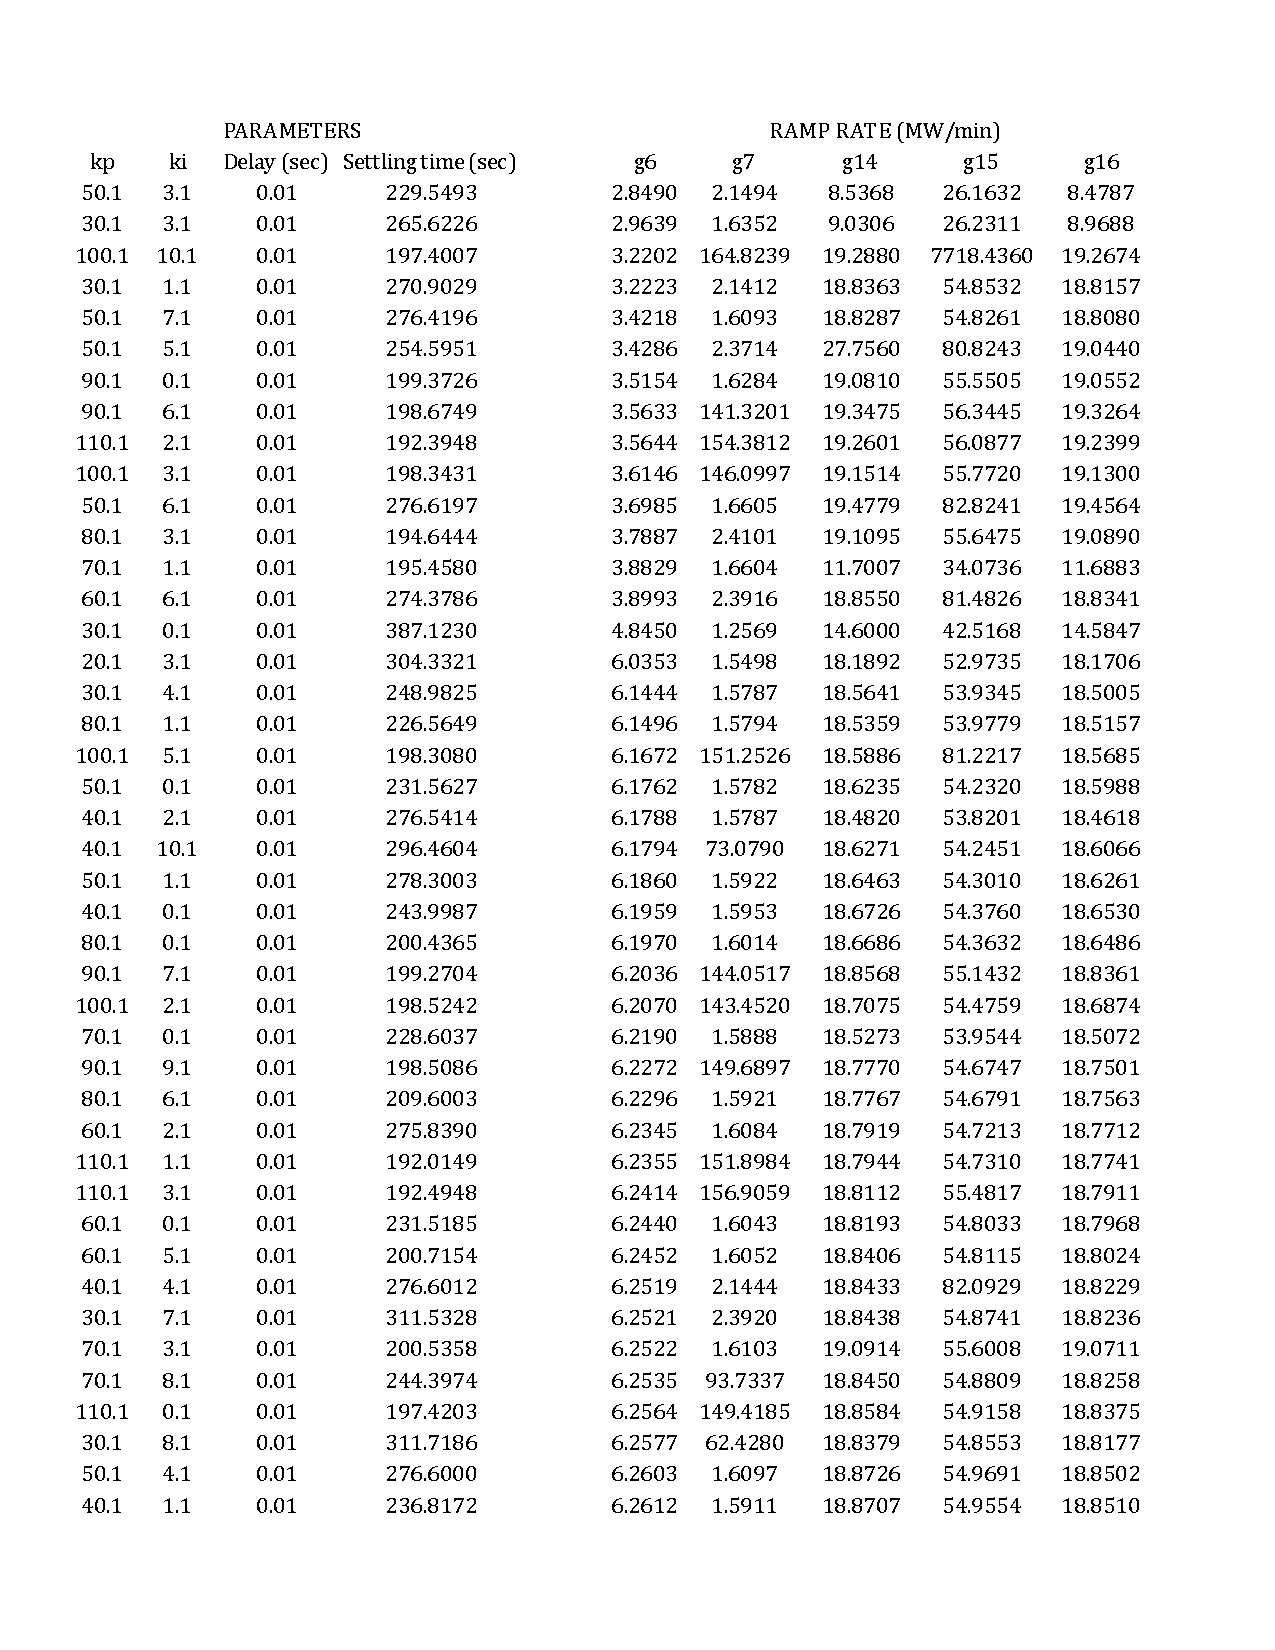
\includegraphics[width = \textwidth]{figure/4_5_risk.pdf}
\caption{Some generators' real ramp rates, ranked by g6's ramp rate.}
\label{4_5_risk}
\end{table*}


Finally, we should have a figure that similar to Figure~\ref{4_4_1_2d}. However, as you can see from Table~\ref{4_5_risk}, none of tuning results can meet the requirement of the limit of ramp rate (i.e. the ramp rates in the test system are larger than the limit). After repeated confirmation, I do not think there are any logic mistake in my algorithm. \\

In fact, our assumption is based on the materials from the United States. Although it's positive to reference an official document, the situation might be different between the United States and Nordic countries.\\

Wärtsilä Oyj Abp, a Finnish corporation which manufactures and services power sources and other equipment in the marine and energy markets, says, \cite{Combustion} "Ramp rates of most industrial frame gas turbine models are advertised as 10 MW/min up to 100 MW/min, with an average of about 25 MW/min". The maximum allowed ramp rate or the average one are significantly larger than the limit we set.\\

Another paper is also mentioned the similar information that, in Germany, \cite{huber2017flexibility} the maximum ramp can be up to 11\%.

Thus, it's reasonable to believe that, in Nordic grid, the official ramp rate should be larger than 1\% of the nominal power per min.\\


Another conclusion that we can sum up from Table~\ref{4_5_risk} is that storage ramp rates are rapid (i.e. output can change quite rapidly). Power devices with a slow response time tend to have a slow ramp rate. This is the philosophical inspiration of Smart Grid operation: a fast response time would exceed the physical limit of a turbine which forces you to slow the response time to keep a balance between the design and the requirement.\\

\chapter{Impact of Time Delay}
\label{Chapter5}
% section:
\section{Hypothesis} %5.1
The hypothesis in this chapter is basically based on the hypothesis in Section~\ref{section4.1}.  \\
 
One of the different hypothesis is that it has several delays here, i.e. delay ranges between 0.01 seconds and 0.21 seconds, and the step is 0.01 seconds.  \\

It allows having the similar hypothesis with Section~\ref{section4.1} because, in this chapter, it can be seen as an extension of last chapter. In the last chapter, Nordic system is tested in a low delay while, in this chapter, we increase the delay. \\ 

An important assumption to allow keeping other parameters the same when increasing the time delay is that a larger time delay declines the performance of Nordic grid.\\
\section{Expected Outcome} %5.2
\label{section5.2}
From the assumption of a larger delay declining the performance of Nordic grid and the results from Section~\ref{section4.4}, I expect in this chapter,\\

\begin{itemize}
    \item The acceptable points will be less if the time delay is increased. \\
    \item To the best result of different delay, kp should be larger when time delay is increased. \\
\end{itemize}


I make this assumption because I think of my experience of waiting for traffic light. At first I didn't notice the green light until the car behind reminded me. In order to make up for the few seconds I missed, I stepped on the accelerator to increase the speed.\\ 

With the same reason, the signal is faced with a time delay problem and it should make up the errors by accelerating the speed of it. Thus, kp will be increased if the time delay is increased. \\
\section{Implement} %5.3
The only difference with Section 4.3 is we need to change the range of time delay. Details are shown as Figure~\ref{5_3_code}.  

\begin{figure}[htbp]
\centering
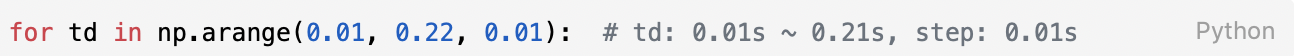
\includegraphics[width = .999\textwidth]{figure/5_3_code.png}
\caption{Implement different time delays}
\label{5_3_code}
\end{figure}
\section{Results} %5.4
\subsection{Results and Analysis} %5.4.1
The final 3D Triangle Surface plot shows in Figure~\ref{5_4_1_Outlier}. 

\begin{figure}[htbp]
\centering
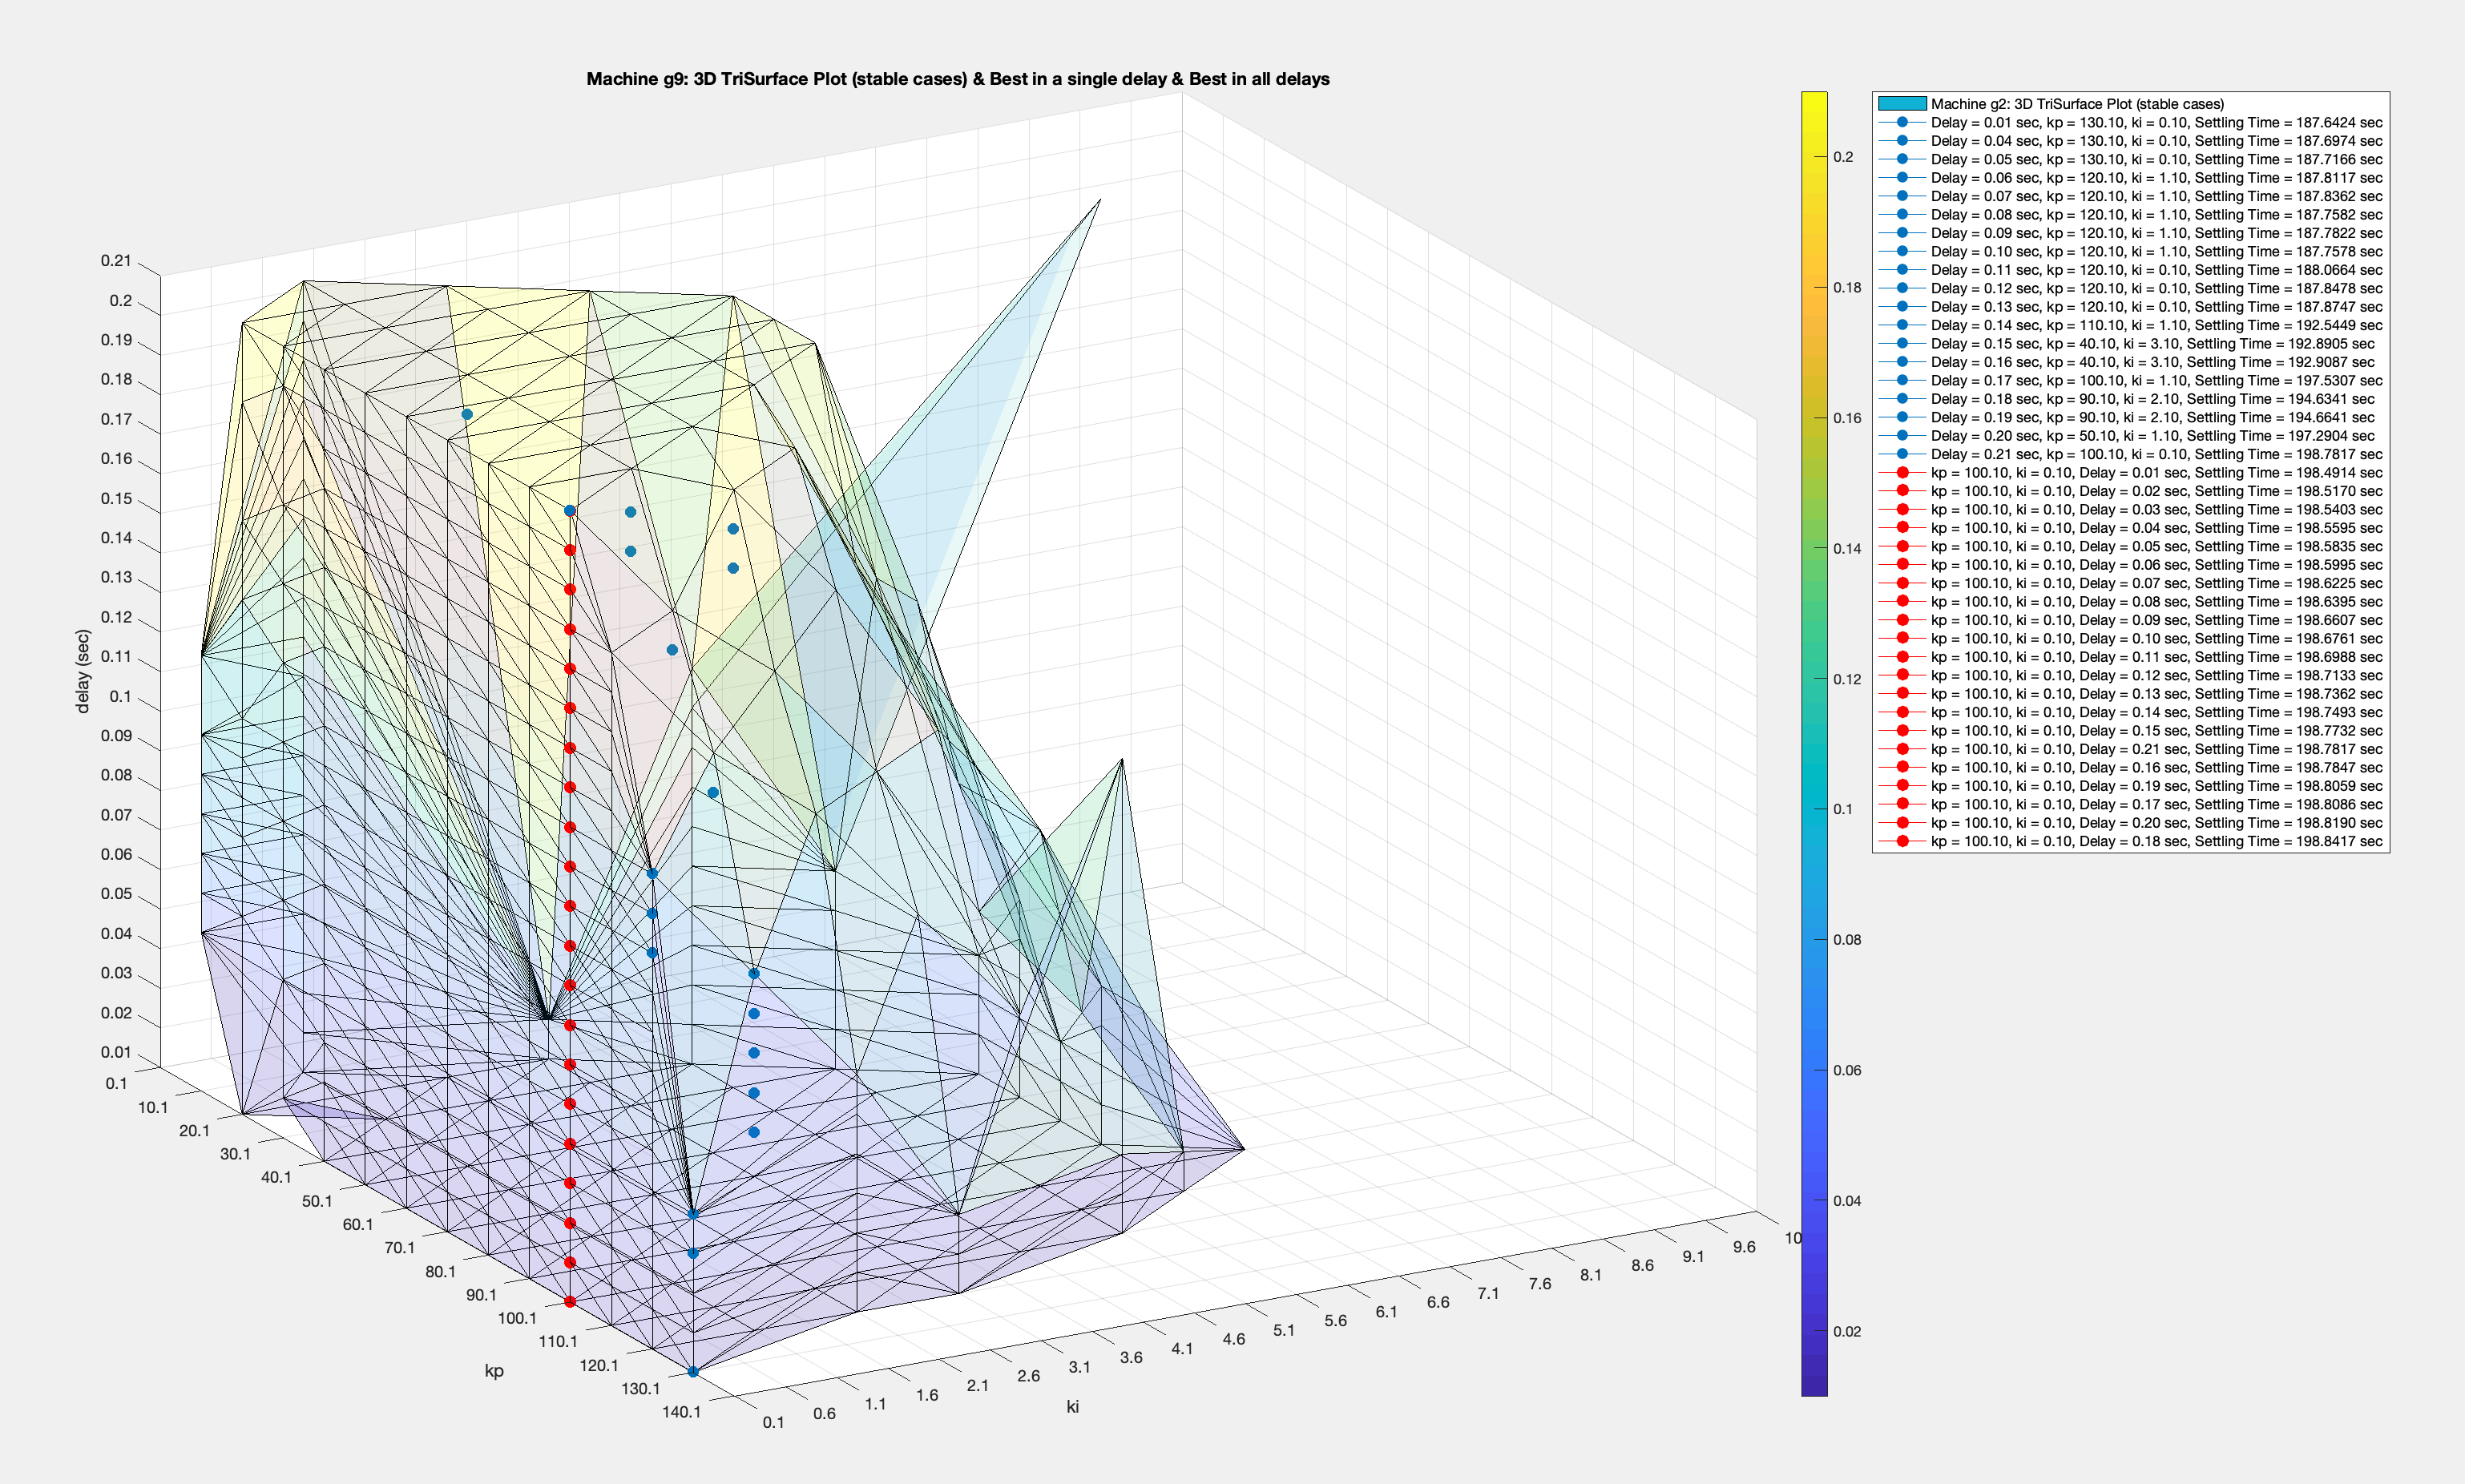
\includegraphics[width = .819\textwidth]{figure/5_4_1_Outlier.png}
\caption{3D plot: contain outliers}
\label{5_4_1_Outlier}
\end{figure}

From Figure~\ref{5_4_1_Outlier}, we can see that there are some outliers here. These outliers can be seen as part of the acceptable results. However, in reality, these outliers can be seen as interference data so we can remove them for a better analysis. 

\begin{figure}[htbp]
\centering
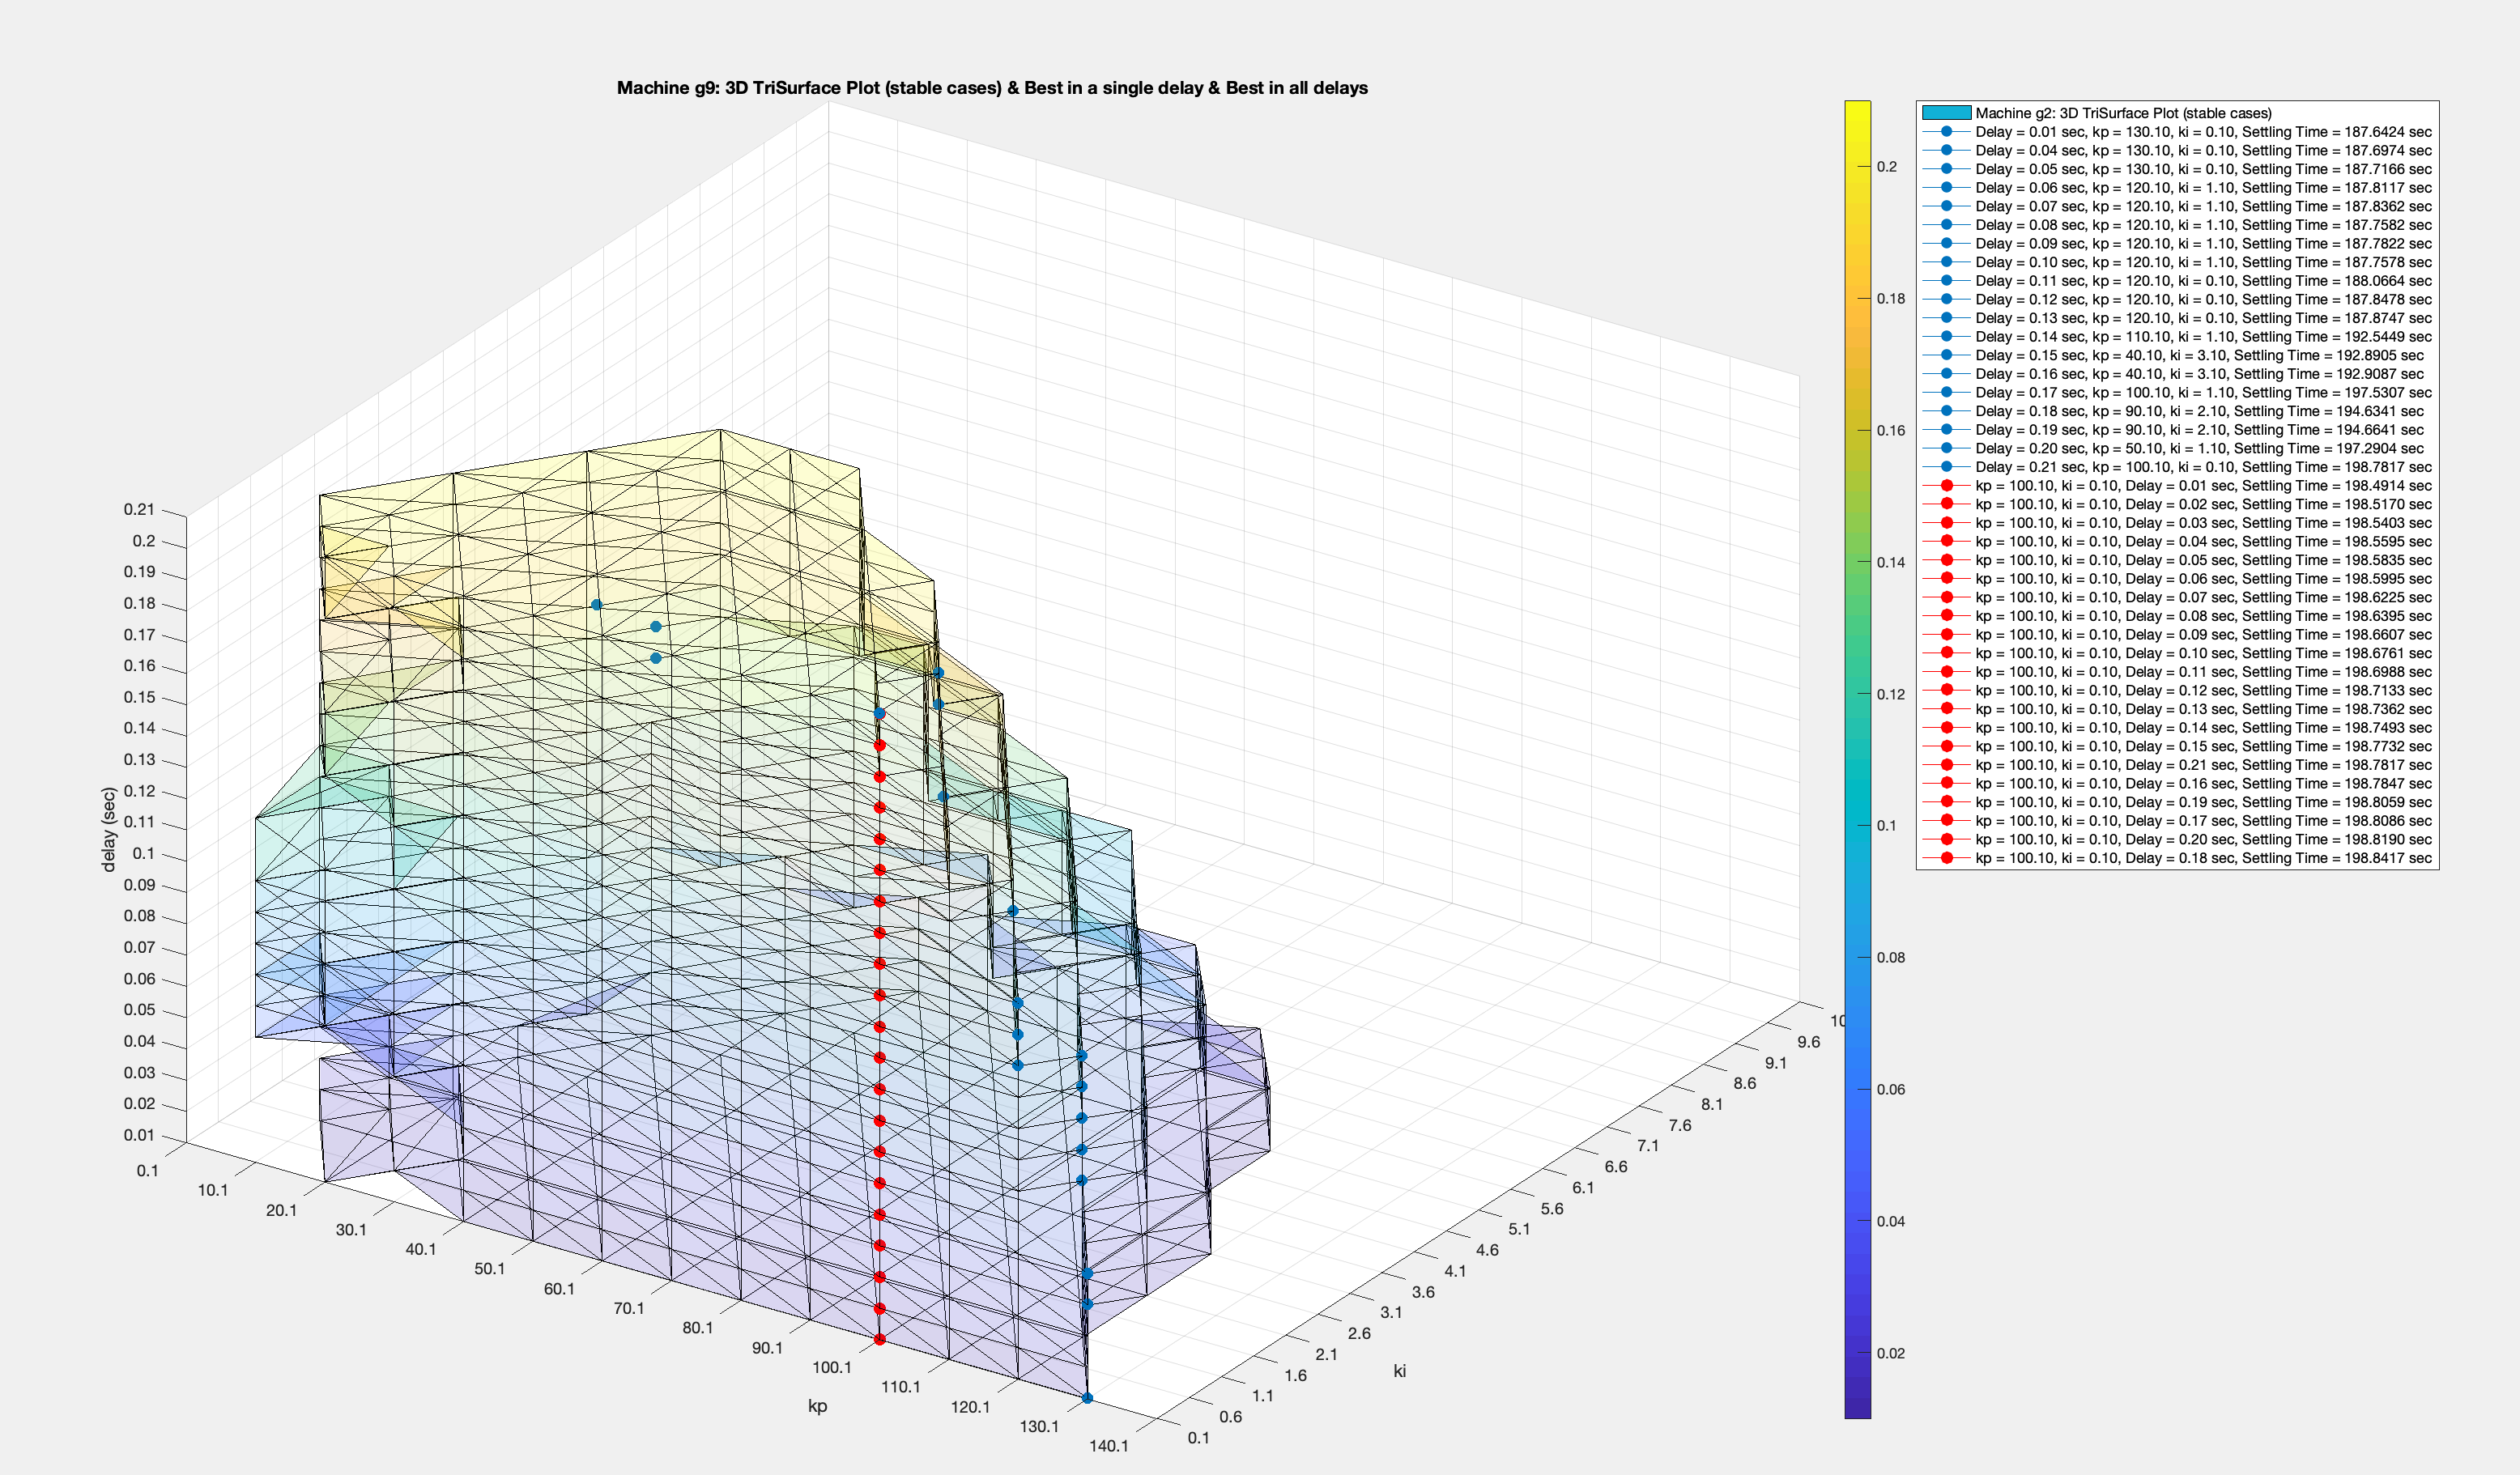
\includegraphics[width = .819\textwidth]{figure/5_4_1_without_Outlier1.png}
\caption{3D plot: contain outliers}
\label{5_4_1_without_Outlier1}
\end{figure}

\begin{figure}[htbp]
\centering
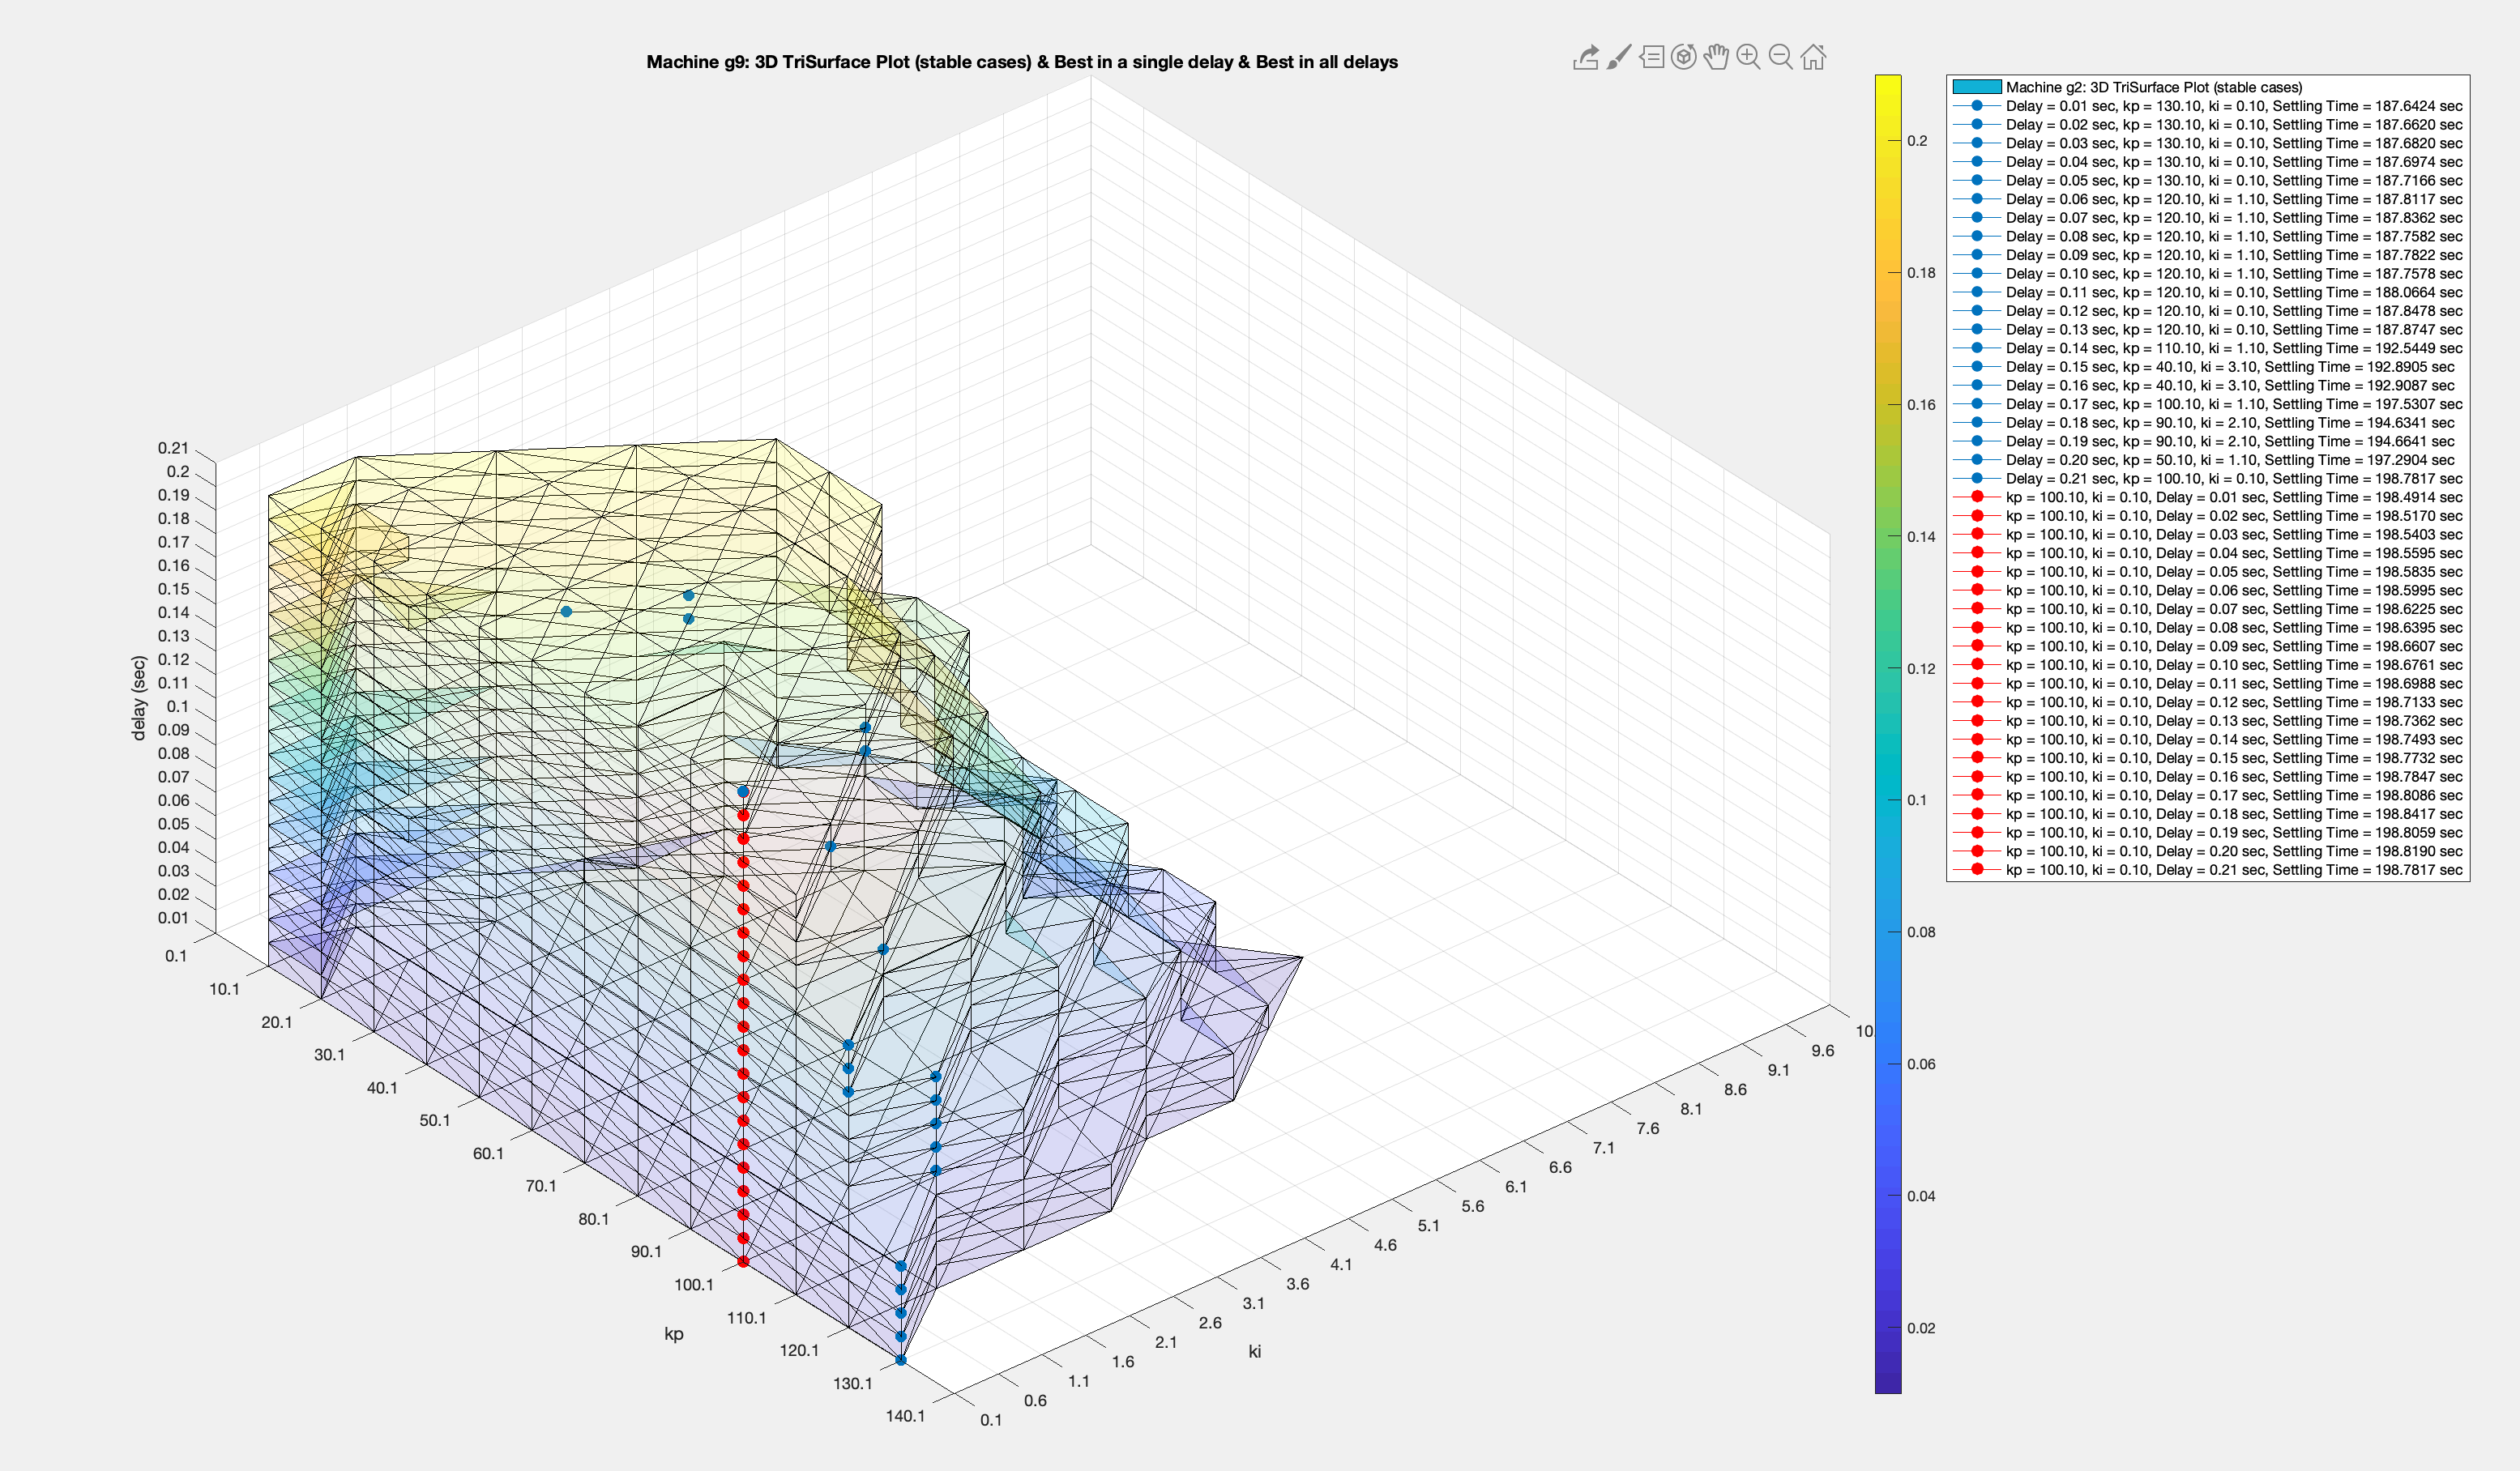
\includegraphics[width = .819\textwidth]{figure/5_4_1_without_Outlier2.png}
\caption{3D plot: contain outliers}
\label{5_4_1_without_Outlier2}
\end{figure}


As we can see from Figure~\ref{5_4_1_without_Outlier1}, overall, the shape of the 3D plot shows kp and ki are shrunk together when the time delay is increased. A increasing time delay removes a larger ki. Detailedly, if the controller has a larger kp and a large ki, the simulation results are recognised as unacceptable points in high probability. If a controller has a high kp but a small ki when the time delay is increased, the simulation results will not be recognised as unacceptable points in a large probability. 

We rank the average settling time for every tuning situation. We finally find that when kp is 100.1 and ki is 0.1, the signal can approach to the nominal value fastest in average. 

Besides, we can find that for the same ki and ki value, for instance, when kp is 100.1 and ki is 0.1, the settling time has a trend of increasing when time delay is increased.  

This directly prove the previous expectation on the impact of the time delay from Section~\ref{section5.2}.  


Another important result is showing in the legend bar in the Figure~\ref{5_4_1_without_Outlier1}. The highlighted blue points are the best result for their delay. For example, “Delay = 0.01 sec, kp = 130.1, ki = 0.10, Settling Time = 187.6424sec” in the legend bar means when time delay is 0.01 seconds, the signal fastest approach to the nominal value if its kp is 130.1 and its ki is 0.10. We find the kp value be increased if time delay is increased. This is in line with the assumption in Section~\ref{section5.2}. 

\subsection{The Best Tuning Result} %5.4.2
\begin{figure}[htbp]
\centering
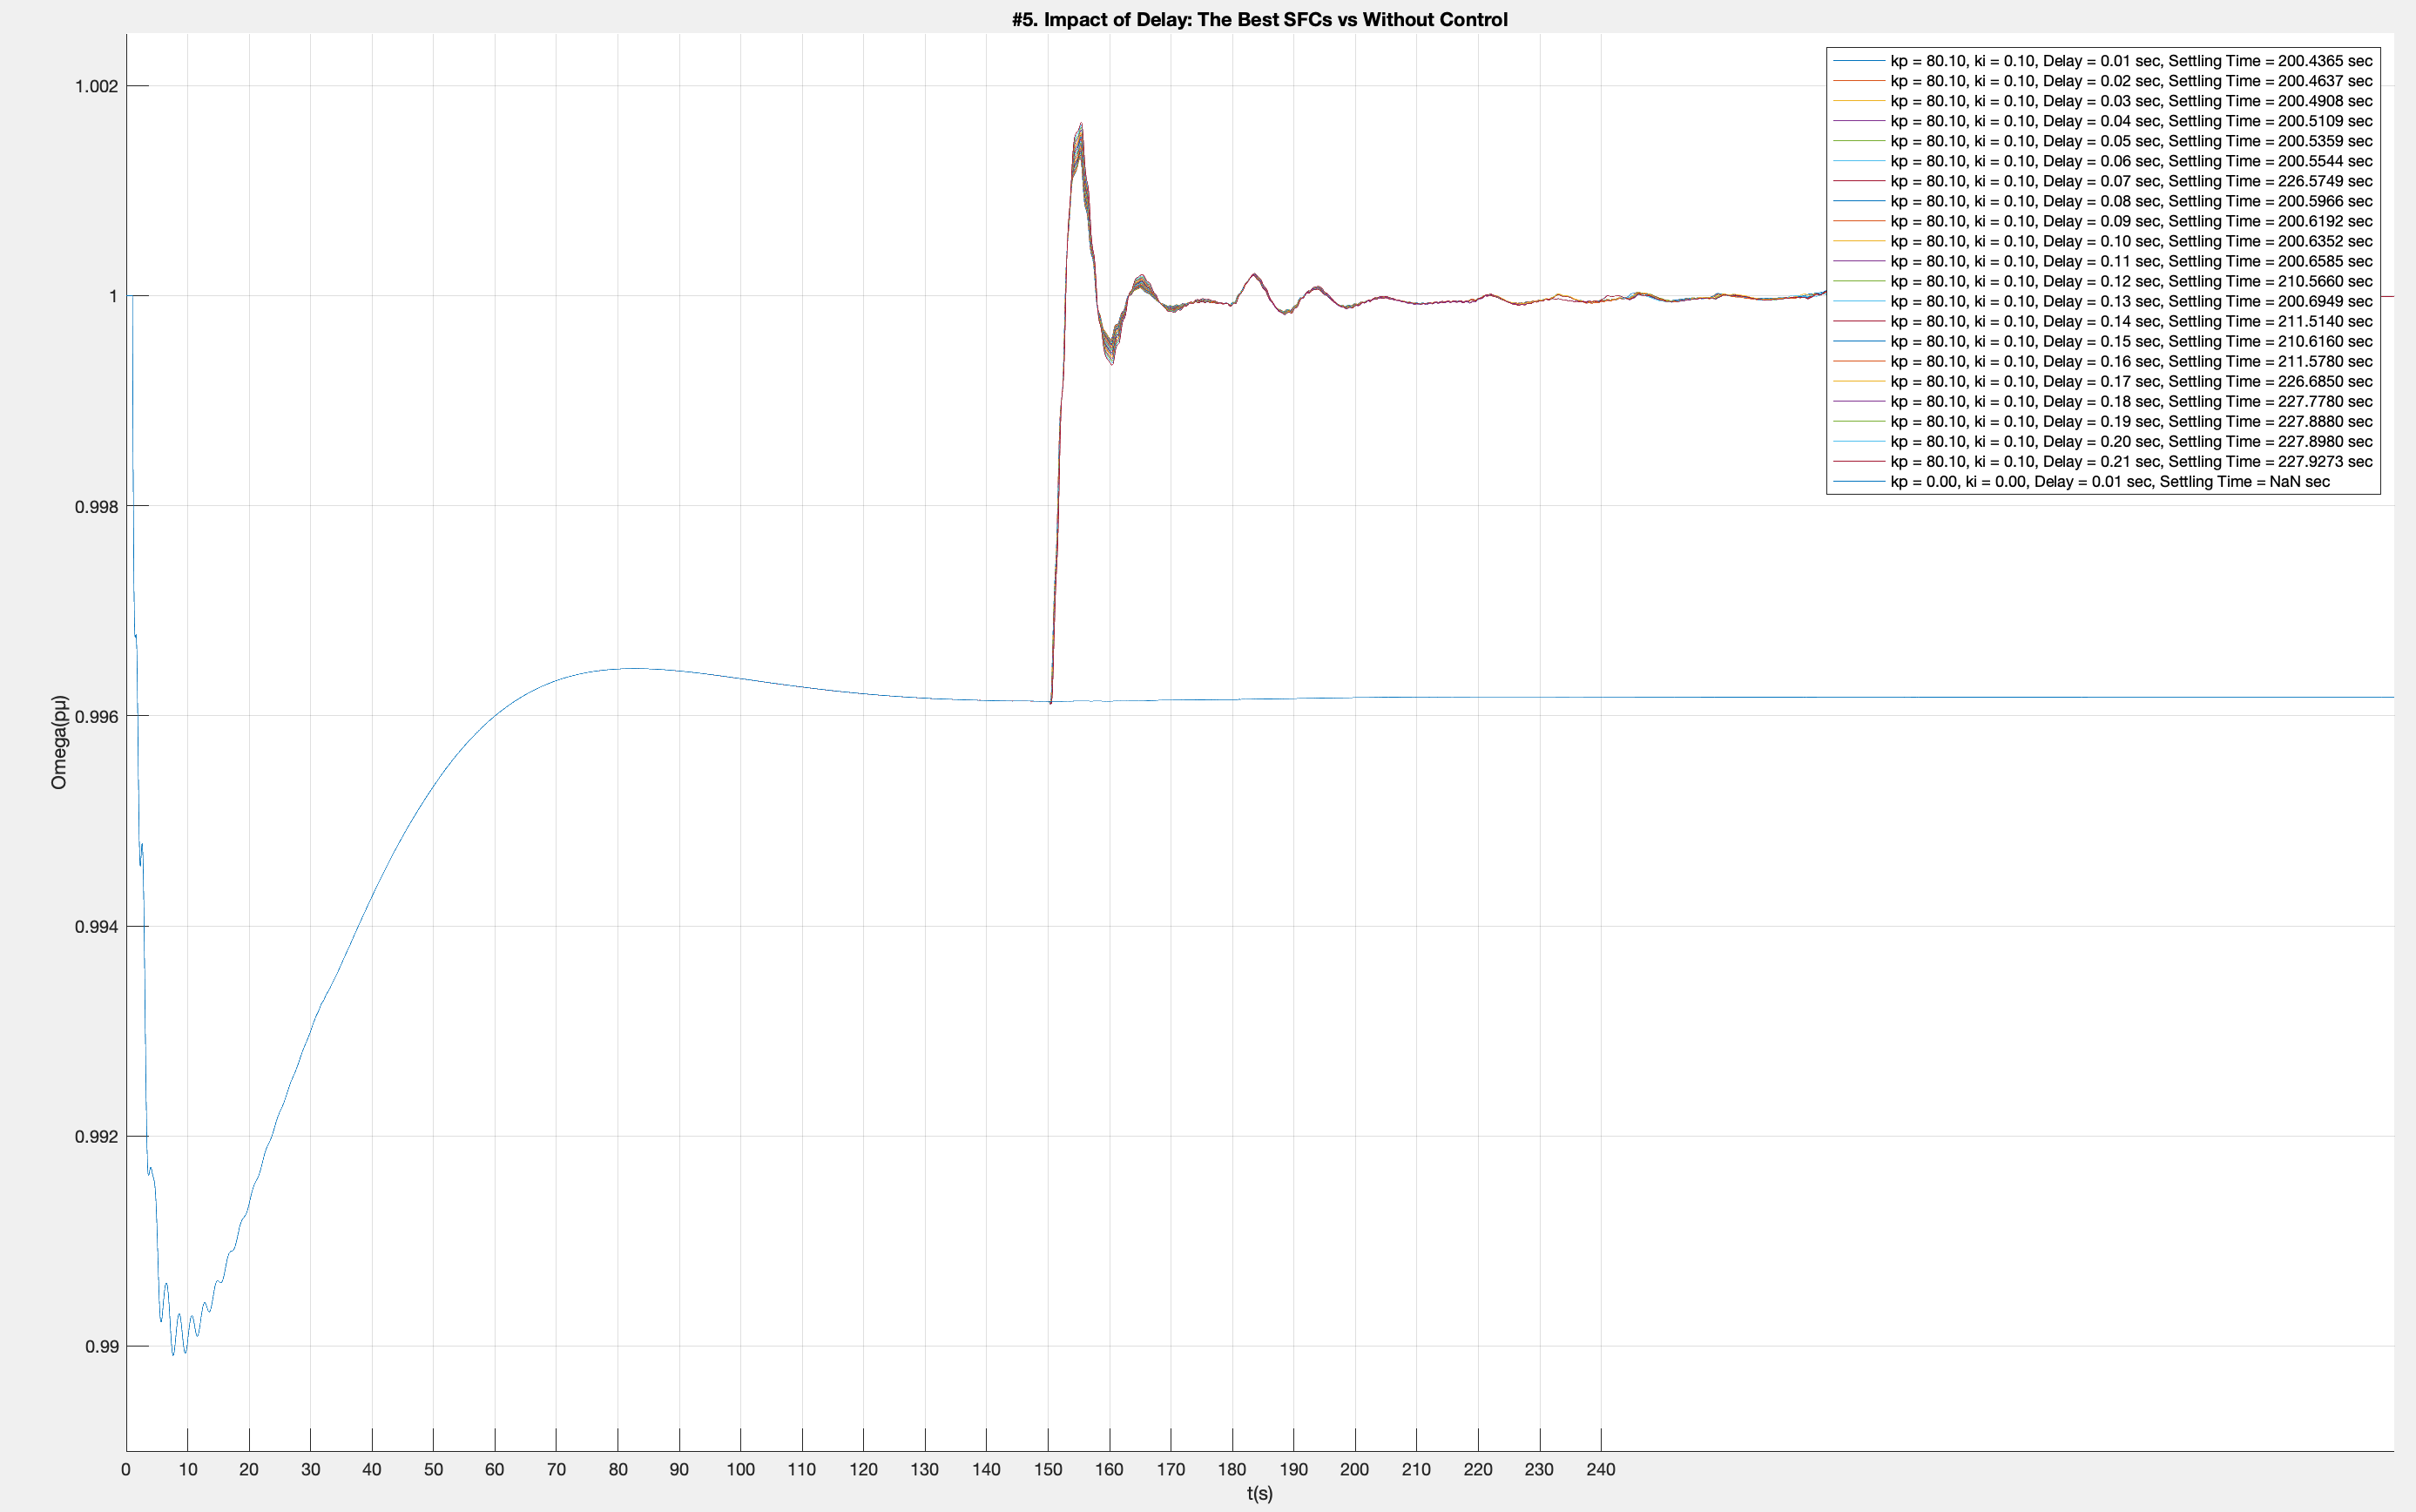
\includegraphics[width = .819\textwidth]{figure/5_4_2.png}
\caption{MATLAB: Impact of Delay: The Best SFCs vs Without Control}
\label{5_4_2}
\end{figure}

\chapter{Emergency Control}
\label{Chapter6}
% section:
\section{Overview} %6.1

Kundur and Morison discussed about emergency control in \sys{Techniques for emergency control of power systems and their implementation}. In that paper, they introduced alert state before describing emergency control. They think, \cite{kundur1997techniques} an alert state will be entered if the security level is below "a certain limit of adequacy", or if the probability of heavy disturb increases due to the weather conditions. However, in an alert state, all constraints are met. Emergency state is at state that one or more constraints are not met. Thus, the emergency control tries to do prevent the emergency state happening and an emergency control will triggered at the alert state.\\

In all, emergency control should be established in emergency conditions to minimise the risk of further uncontrolled separation, loss of generation, or system shutdown. In reality, \cite{kundur1997techniques} alert thresholds can be established. If the system exceeds one of the alert thresholds, emergency control can start.\\

In our case, emergency control starts from the lowest point of frequency in Primary Frequency Control and use Secondary Frequency Control to restore its frequency to prevent the risk of black out.
\section{Hypothesis and Implement} %6.2
Referencing Figure~\ref{4_1_1_without2} in Subsection~\ref{subsection4.1.1}, we find one of the lowest point, as shown in the Figure~\ref{6_2_g9}, as our start point of Emergency Control.  

\begin{figure}[htbp]
\centering
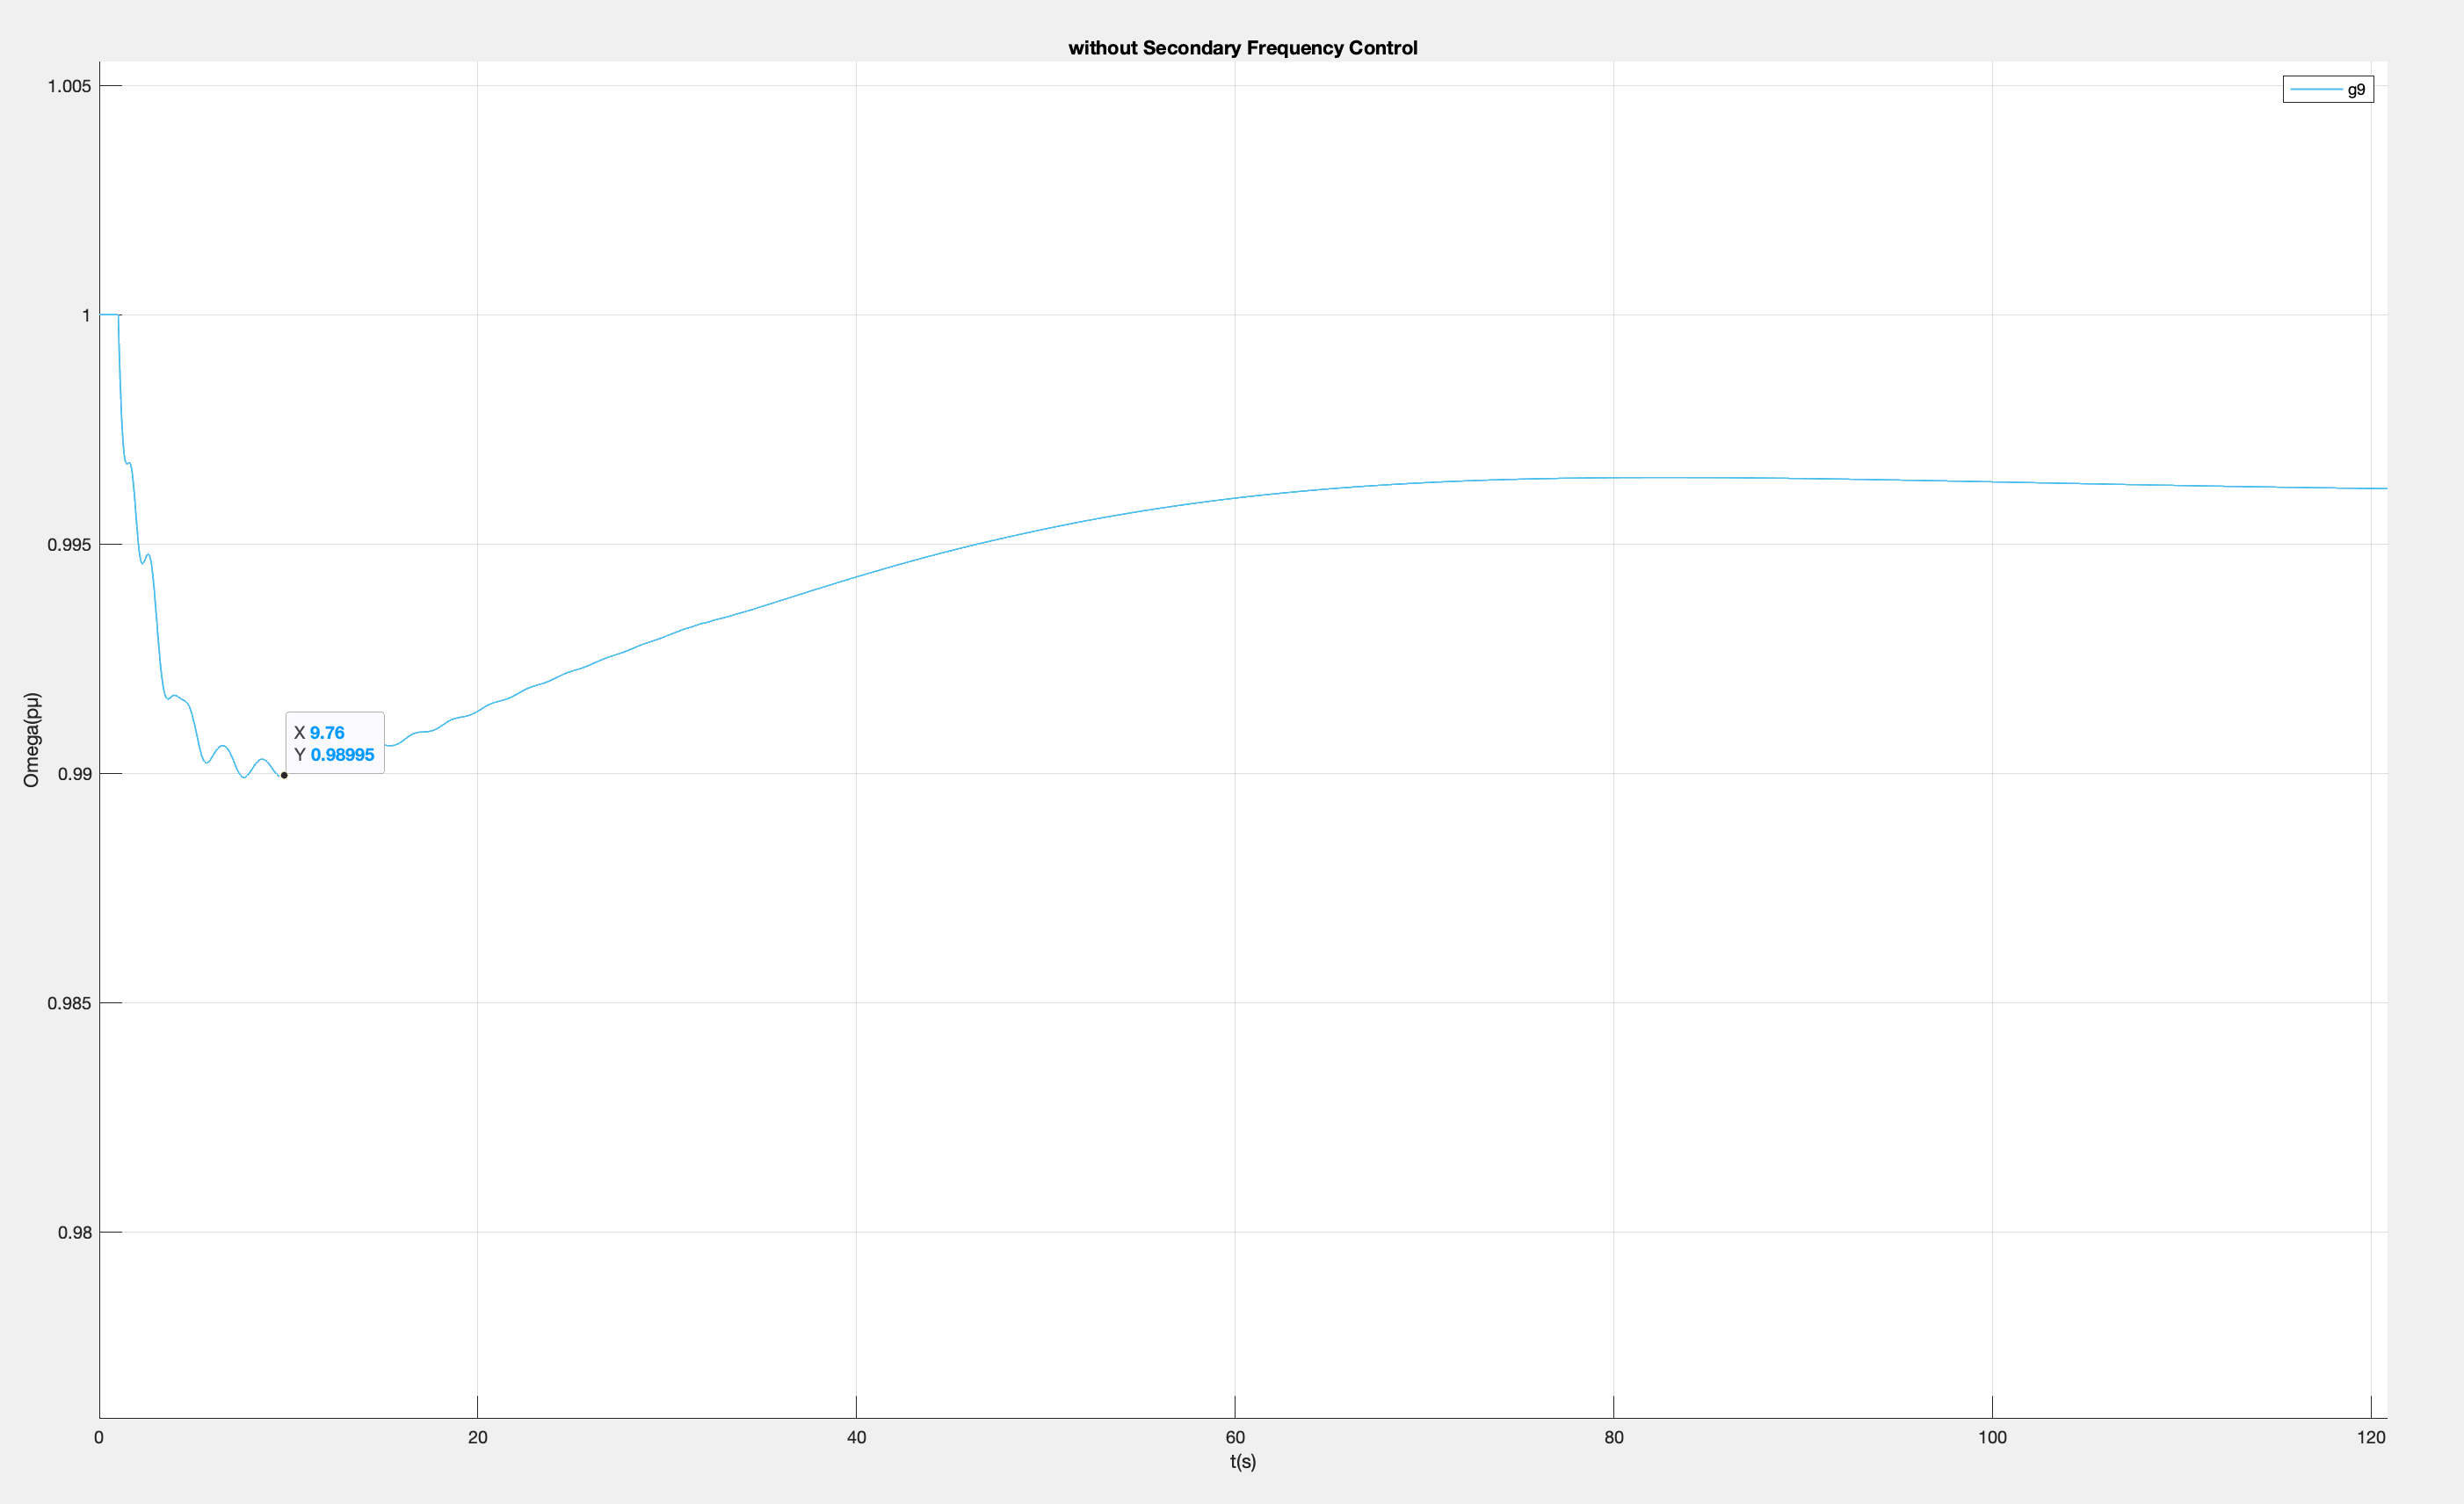
\includegraphics[width = .819\textwidth]{figure/6_2_g9.png}
\caption{Start time of Emergency Control.}
\label{6_2_g9}
\end{figure}

We start the Emergency Control from the 9.76th second and use one of the acceptable tuning results, i.e. kp is 30.1 and ki is 0.1, in Chapter~\ref{Chapter4}. The aim of such hypotheses is to test the impact of time delay under the condition of Emergency Control. The simulation lasts for 360 seconds. 
\section{Expected Outcome} %6.3
Time delay disturbs the system. A faster controller be implemented for a larger time delay to eliminate the errors due to the time delay. We already have a detailed discussion in Chapter~\ref{Chapter5}. In all, emergency control should not change the conclusion on the impact of time delay although they have different start time and have different performance under the same tuning condition. 
\section{Results} % 6.4
\subsection{Results and Analysis} %6.4.1

All the acceptable results can be seen as Figure~\ref{6_4_i}. Compared to Figure~\ref{5_4_1_i}, we can see there are less acceptable tuning results in the emergency control.\\

Separately, when delay is 0.01 seconds, as shown in Figure~\ref{6_4_i} and in Figure~\ref{6_4_copare_01}, there are only four acceptable results for the emergency control. Besides, emergency control removes high-kp values to make sure the overshoot is in the set range.

Comparing Figure~\ref{6_4_CompaPlots_01}, Figure~\ref{6_4_CompaPlots_11} and Figure~\ref{6_4_CompaPlots_21}, the system is more unstable when the time delay increases.

\begin{figure}[htbp]
\centering
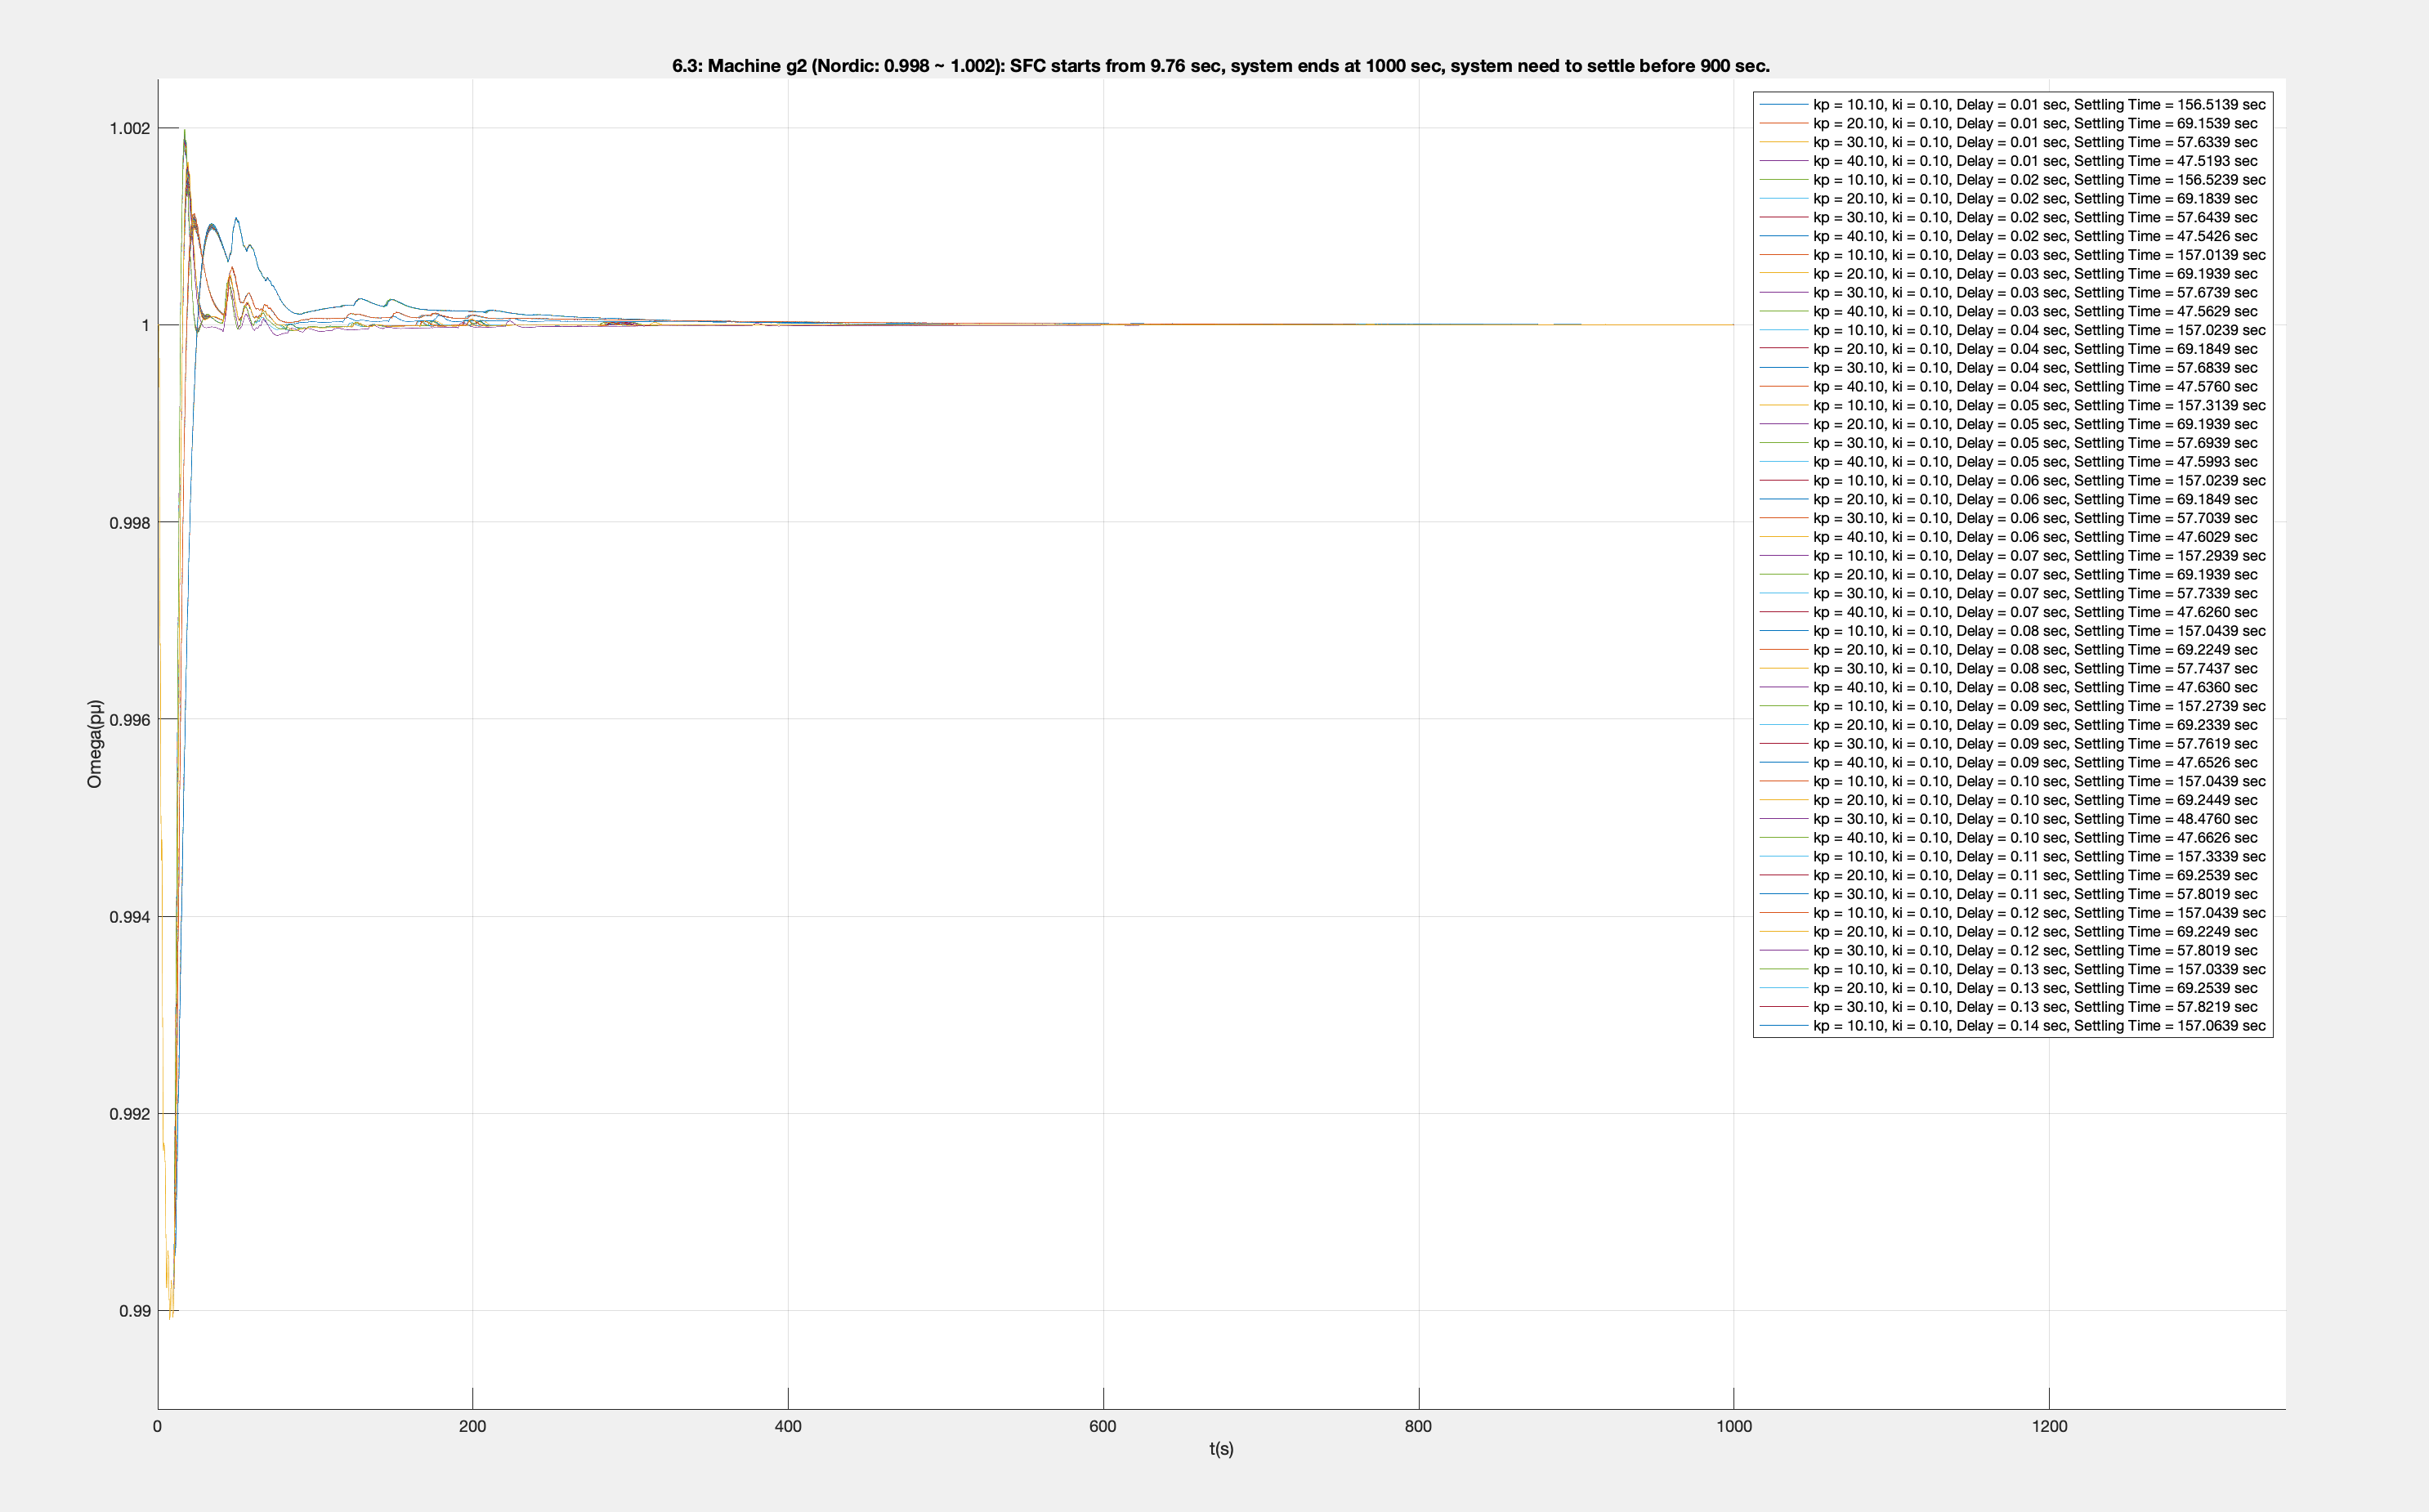
\includegraphics[width = .891\textwidth]{figure/6_4_i.png}
\caption{Acceptable results of Emergency Control.}
\label{6_4_i}
\end{figure}

\begin{figure}[htbp]
\centering
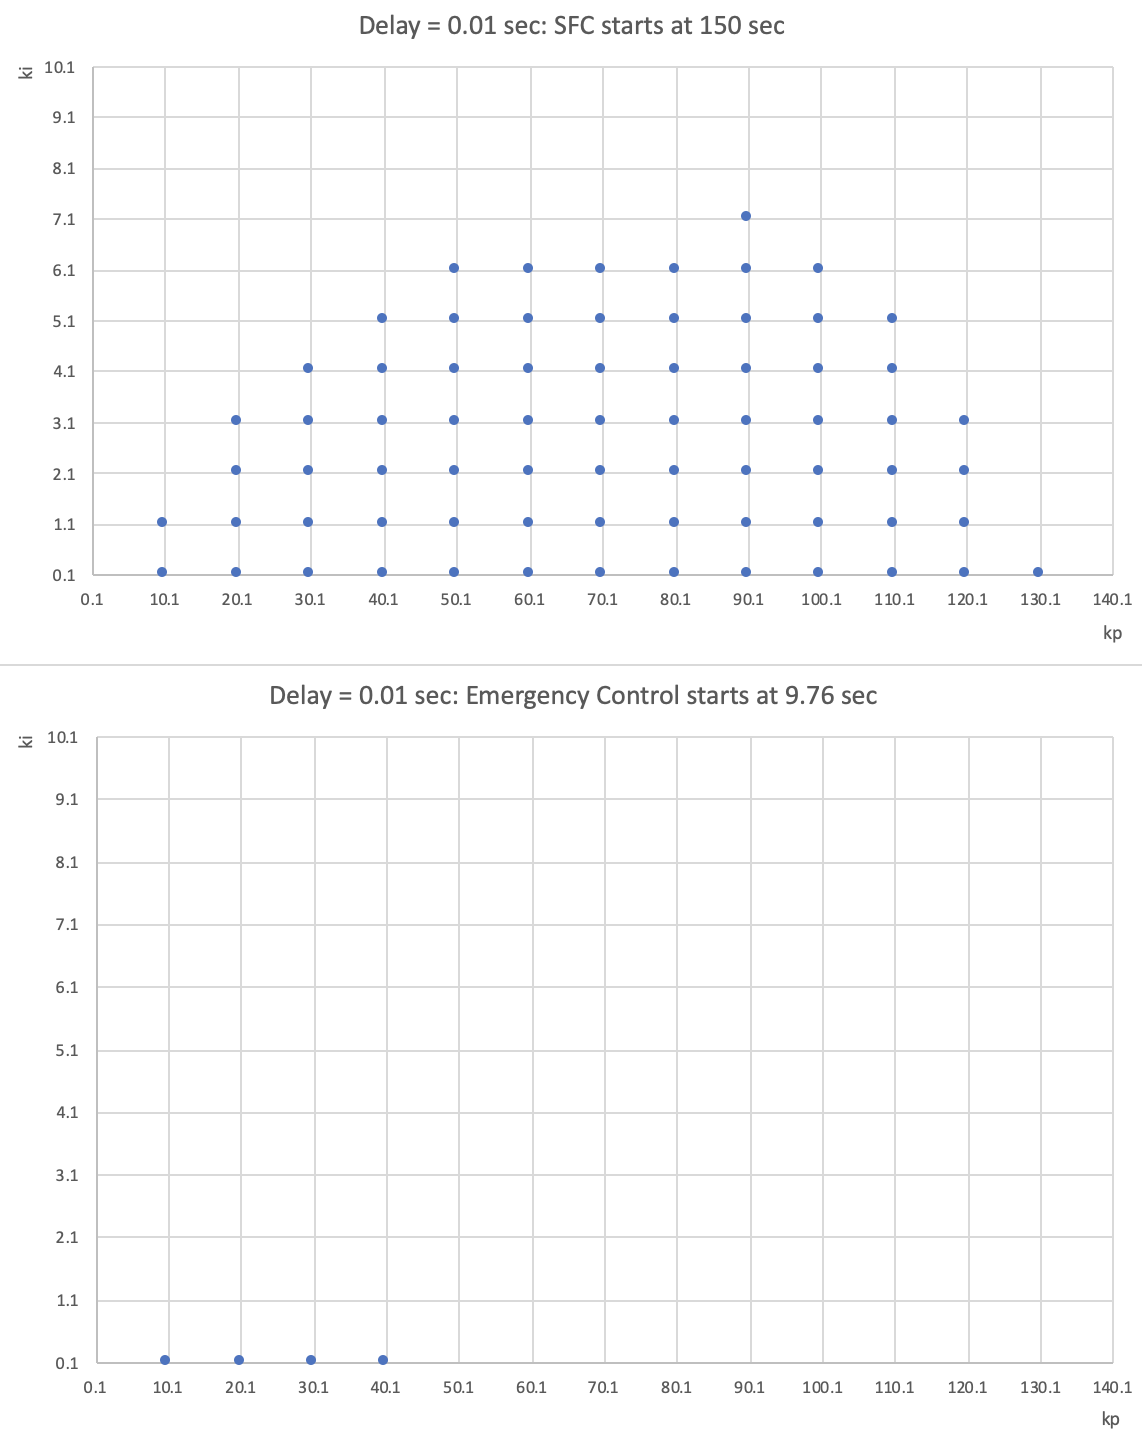
\includegraphics[width = .891\textwidth]{figure/6_4_copare_01.png}
\caption{Comparison: Delay is 0.01 sec}
\label{6_4_copare_01}
\end{figure}

\begin{figure}[htbp]
\centering
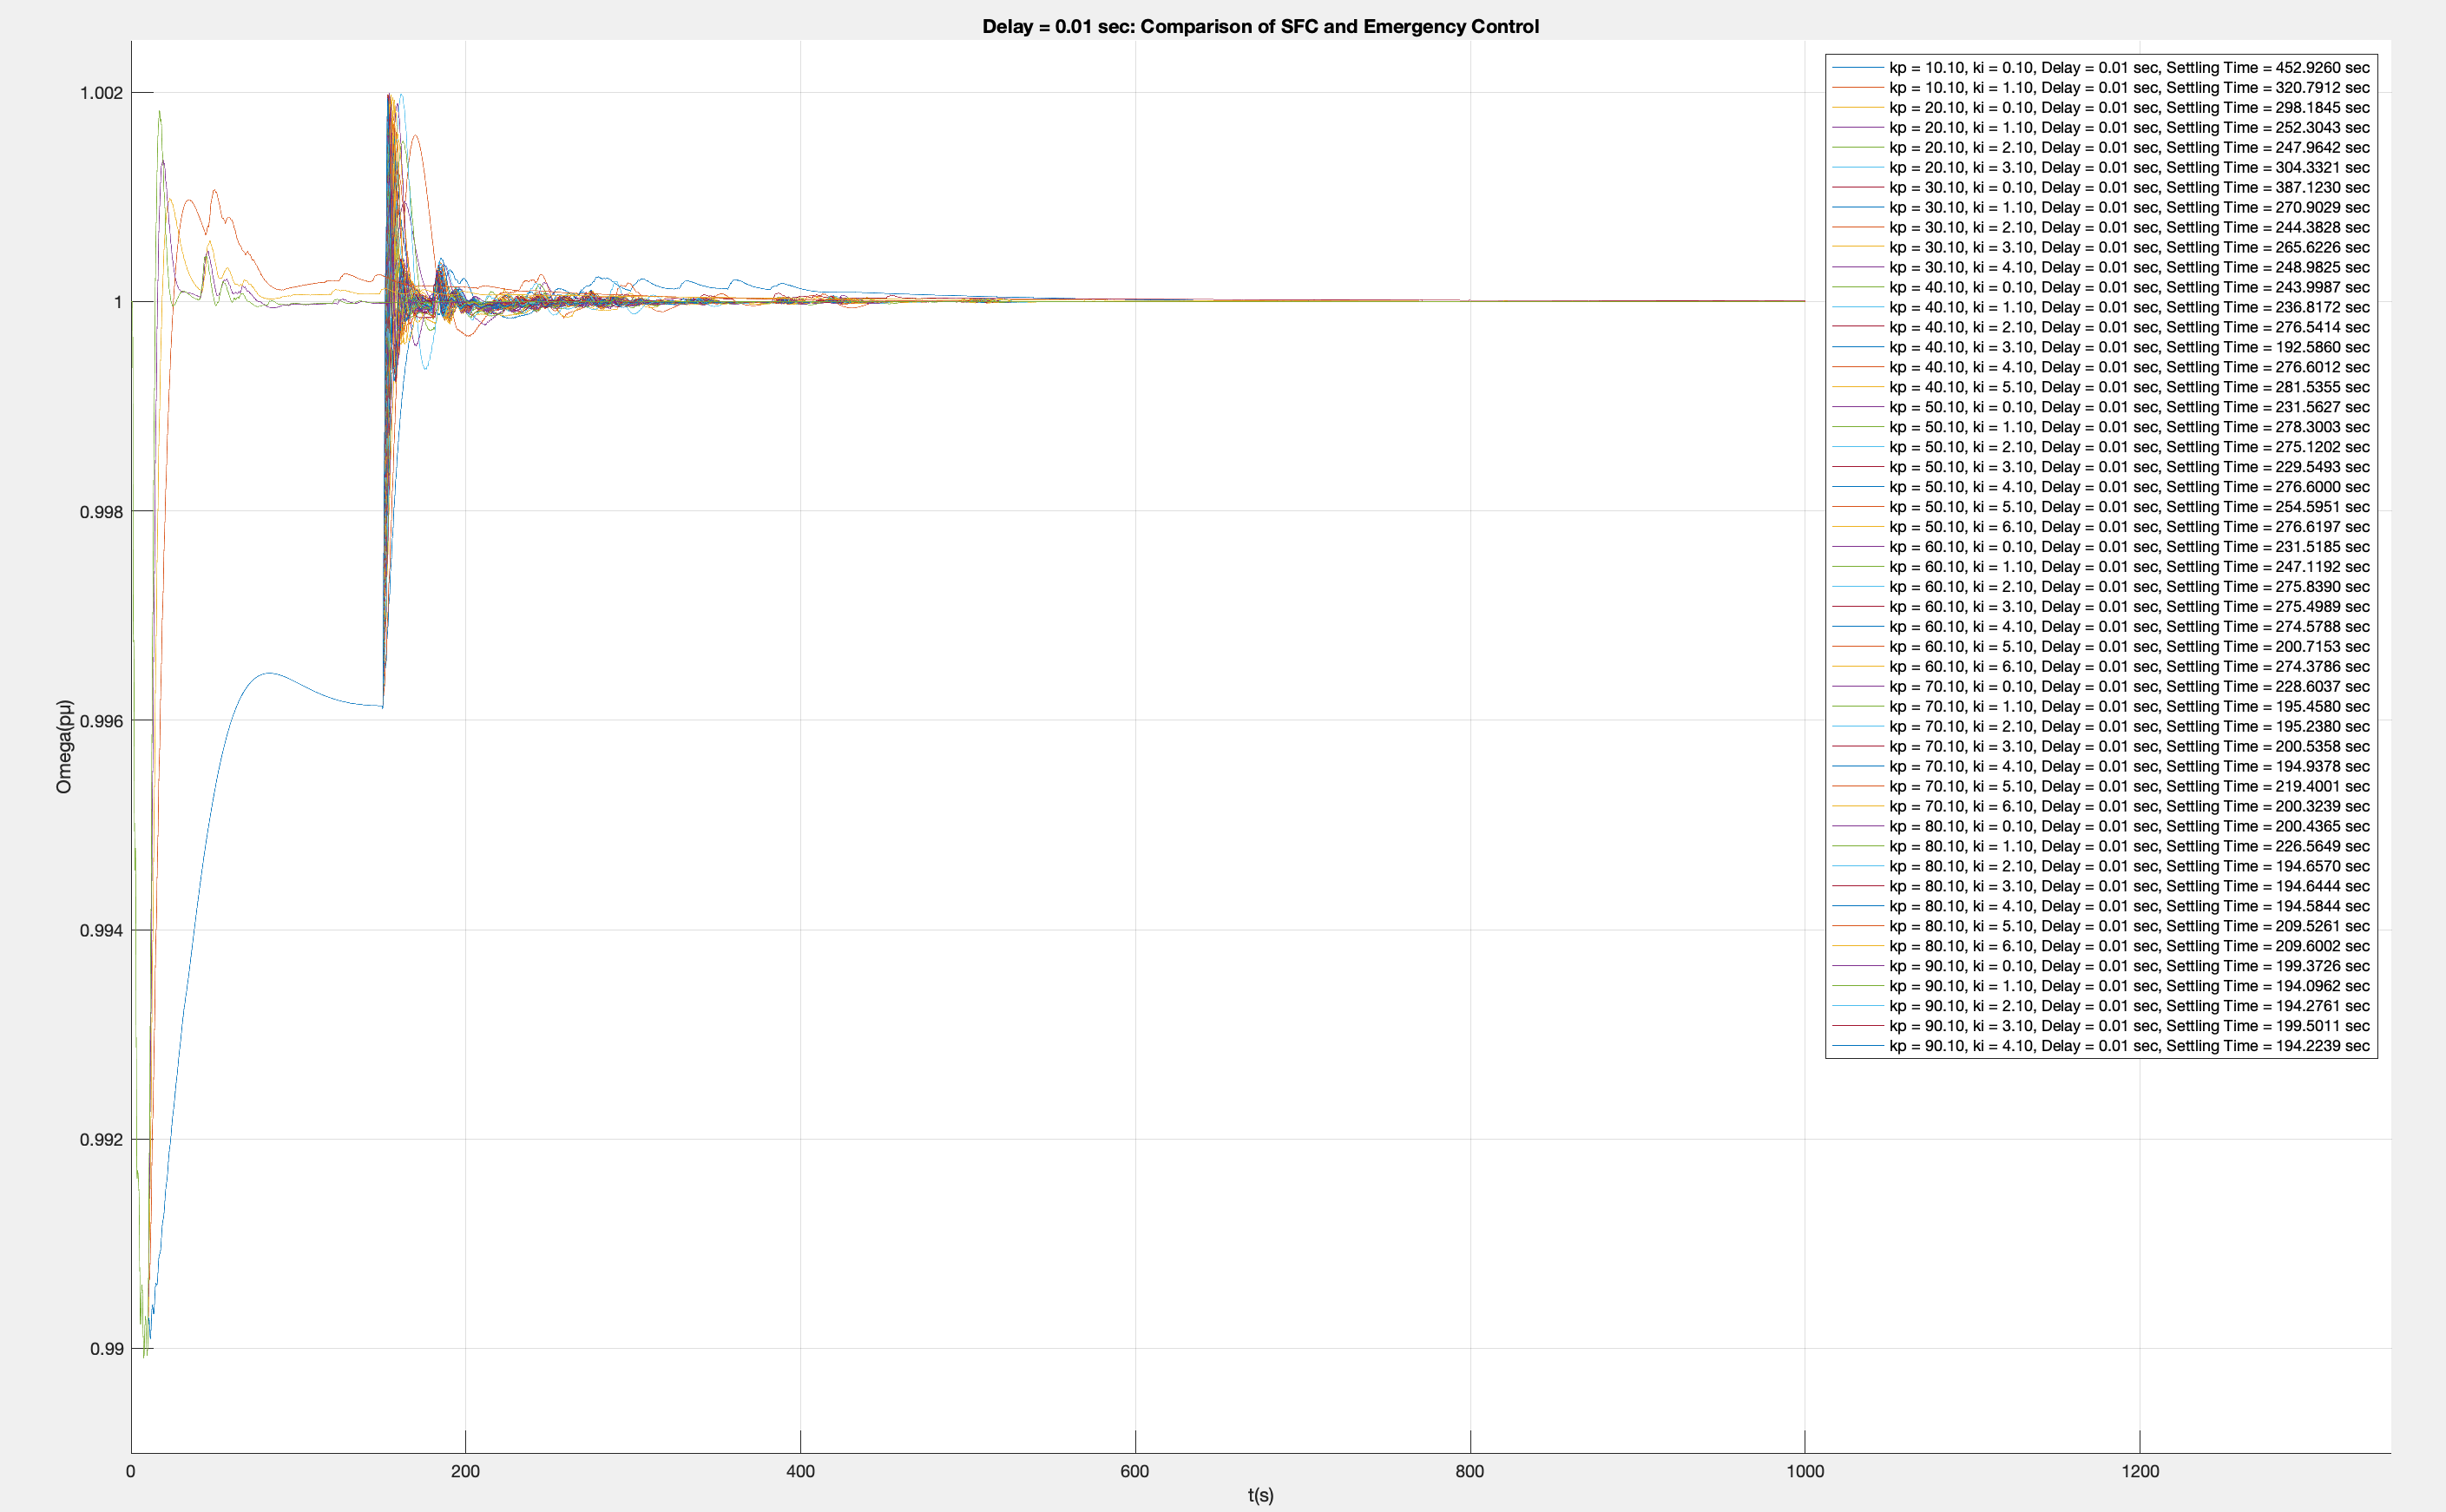
\includegraphics[width = .891\textwidth]{figure/6_4_CompaPlots_01.png}
\caption{Sketches for SFC and Emergency Control: Delay is 0.01 sec}
\label{6_4_CompaPlots_01}
\end{figure}


\begin{figure}[htbp]
\centering
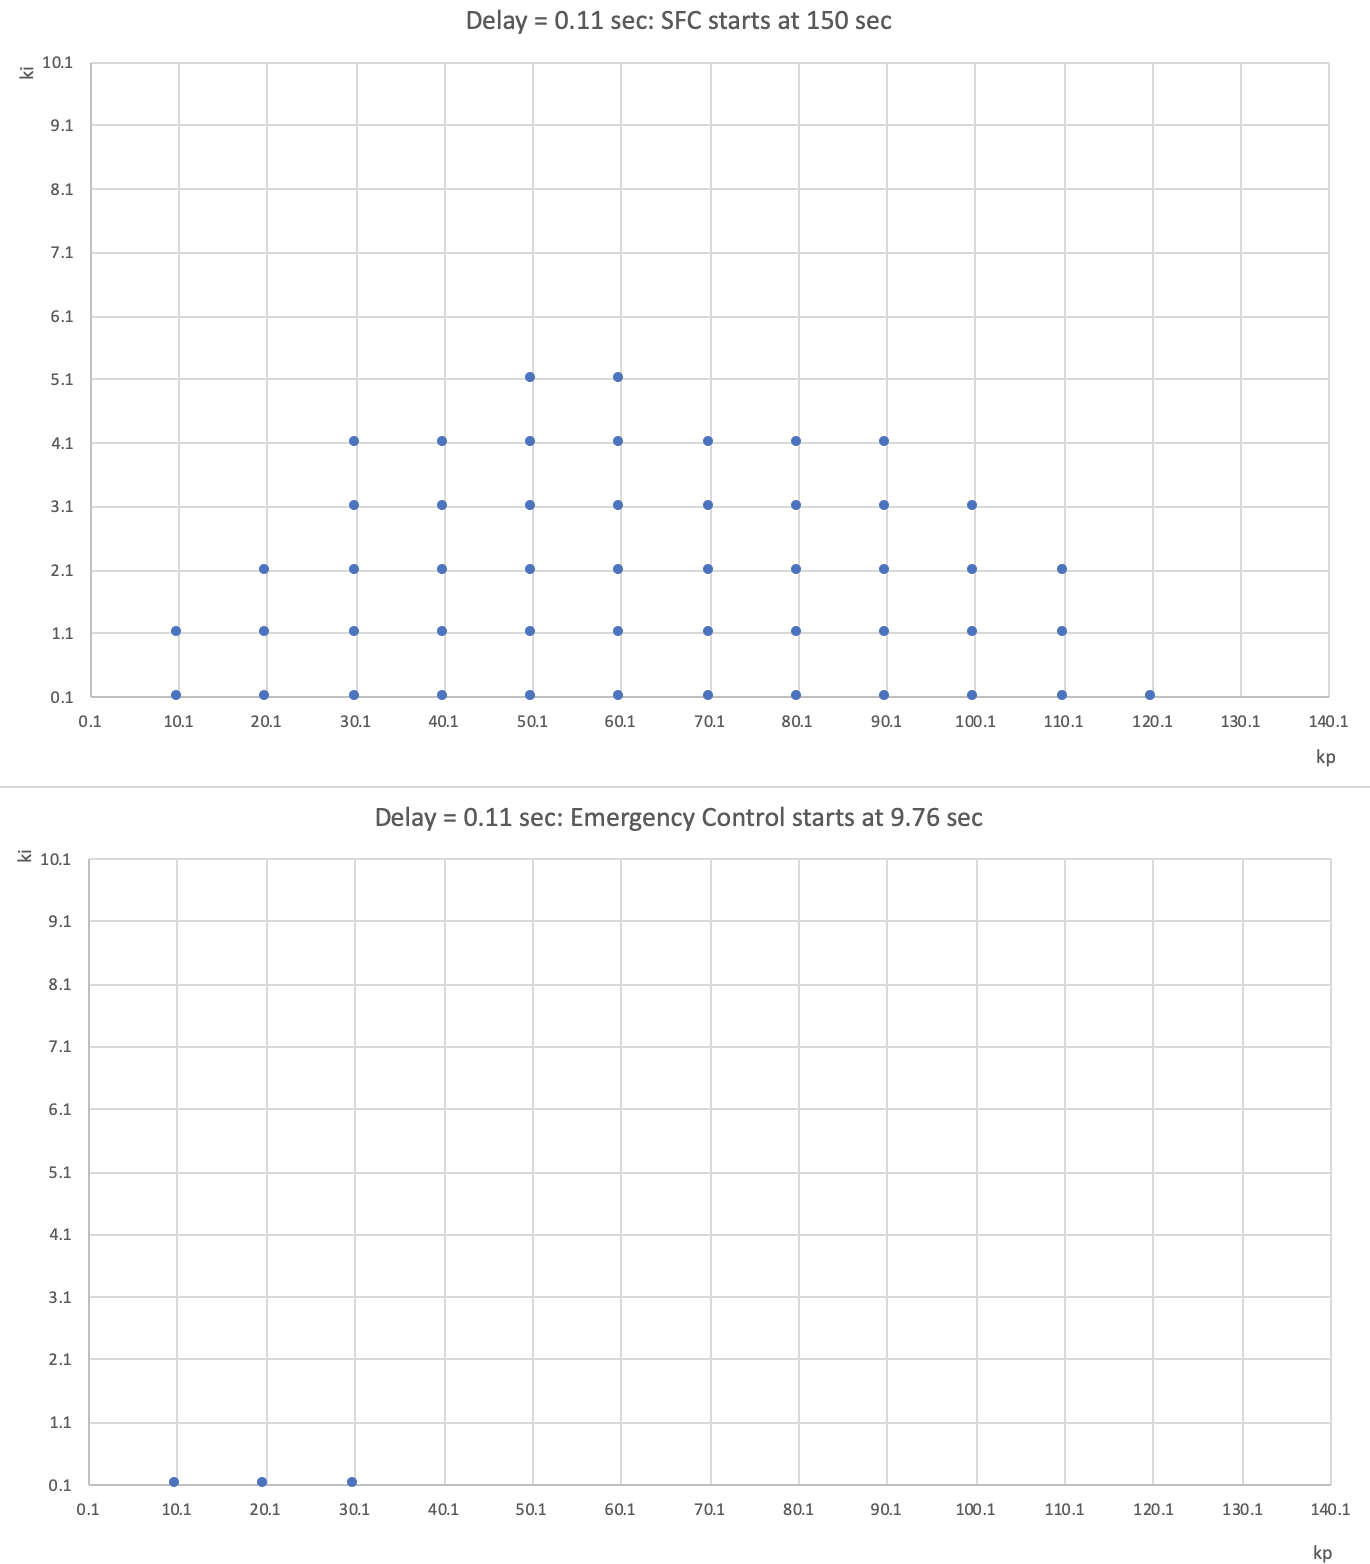
\includegraphics[width = .891\textwidth]{figure/6_4_copare_11.png}
\caption{Comparison: Delay is 0.11 sec}
\label{6_4_copare_11}
\end{figure}


\begin{figure}[htbp]
\centering
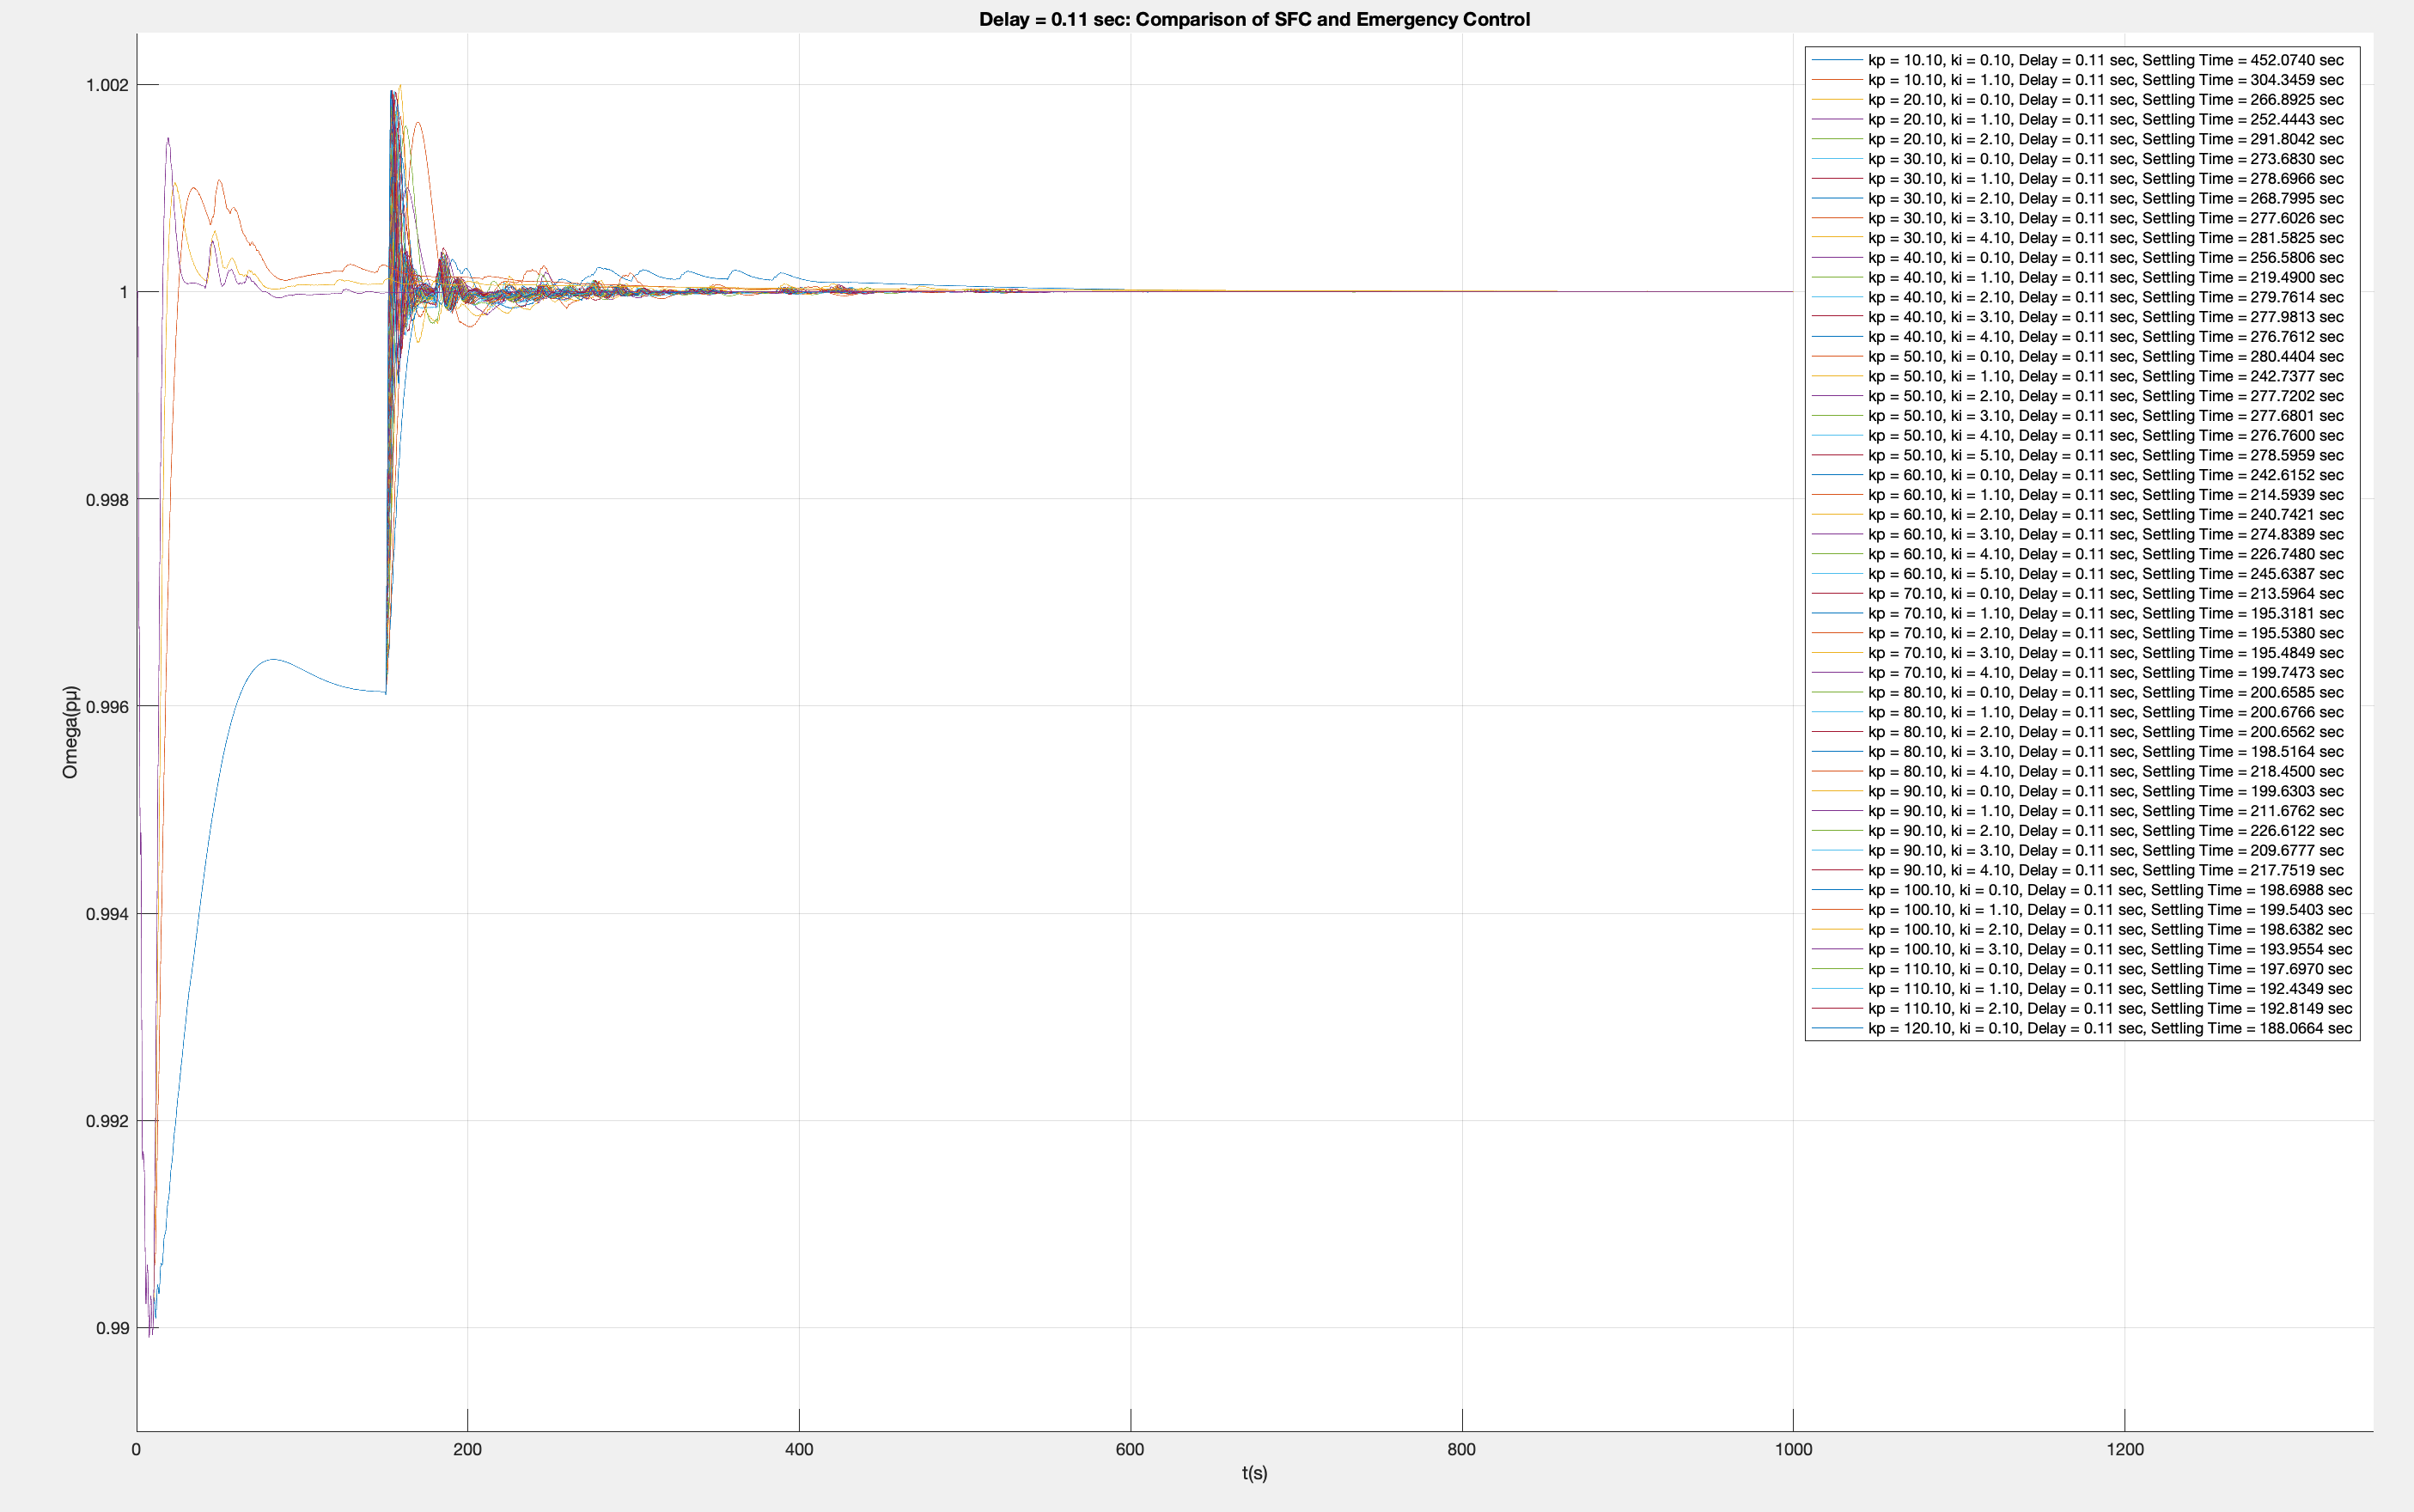
\includegraphics[width = .891\textwidth]{figure/6_4_CompaPlots_11.png}
\caption{Sketches for SFC and Emergency Control: Delay is 0.11 sec}
\label{6_4_CompaPlots_11}
\end{figure}


\begin{figure}[htbp]
\centering
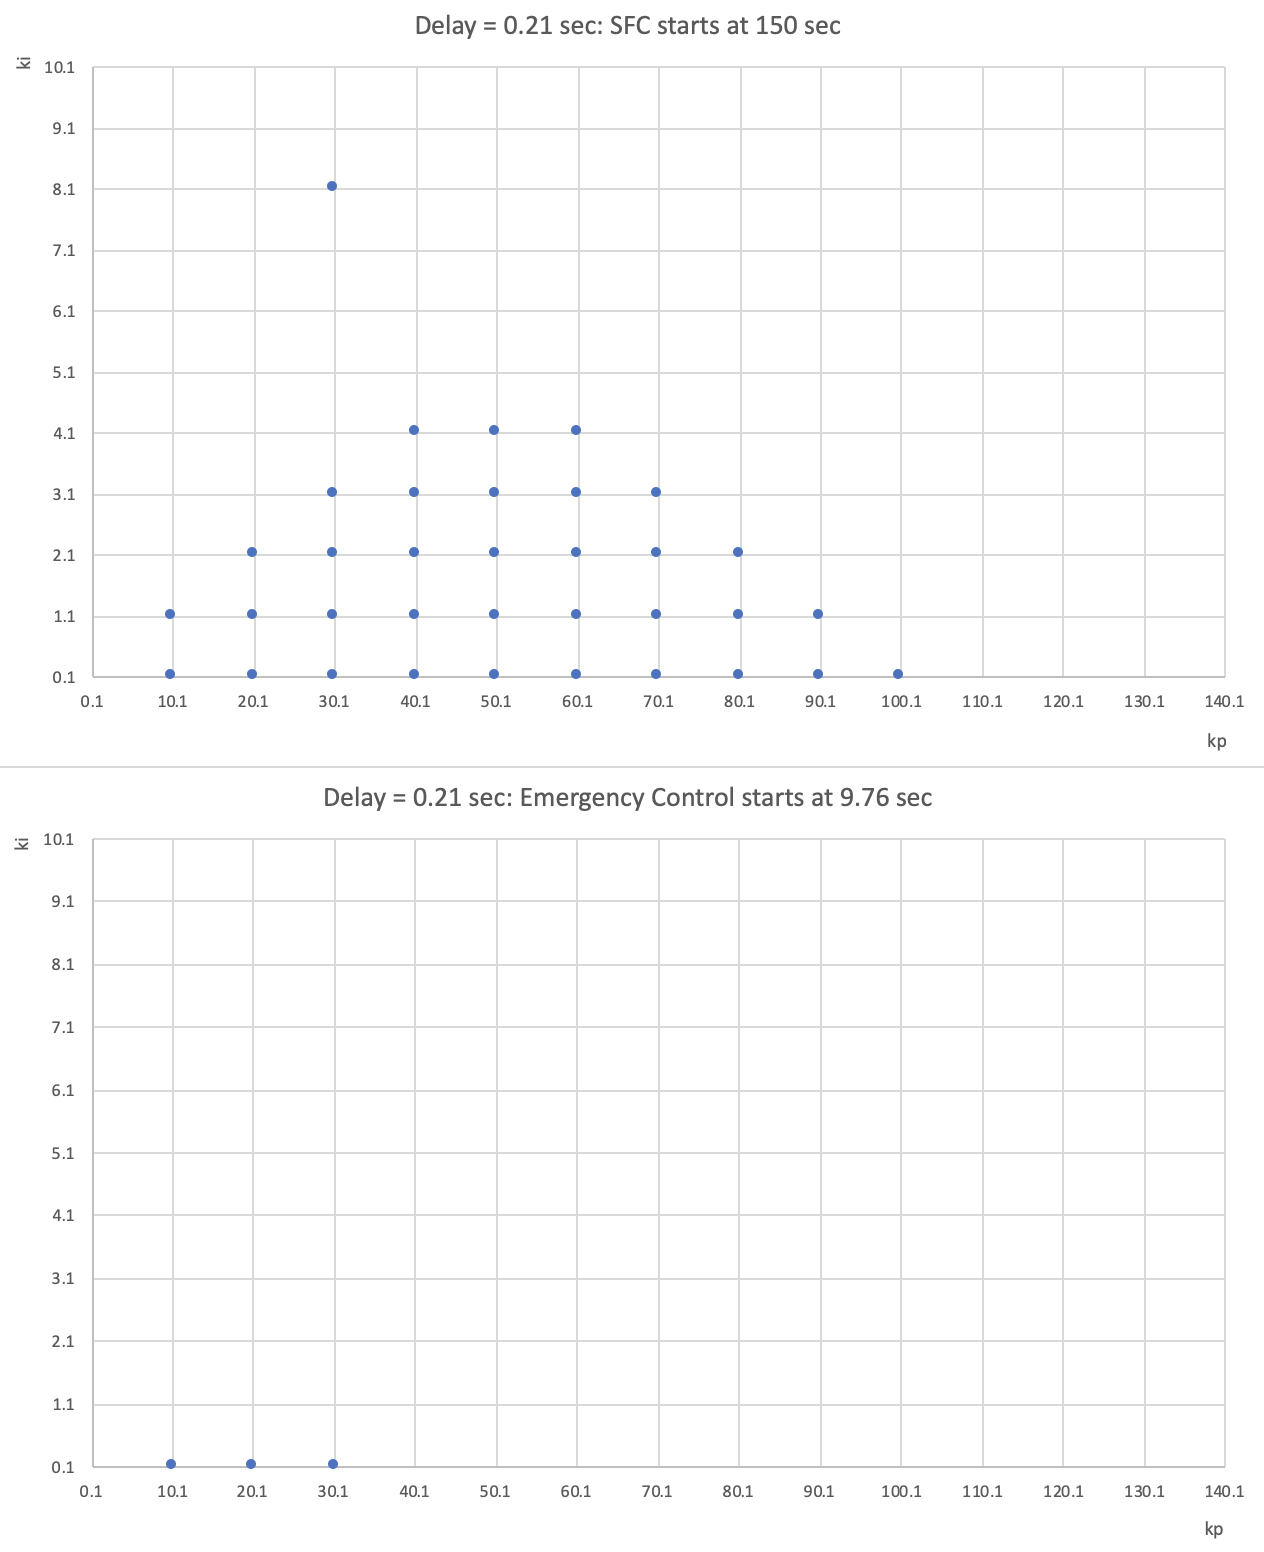
\includegraphics[width = .891\textwidth]{figure/6_4_copare_21.png}
\caption{Comparison: Delay is 0.21 sec}
\label{6_4_copare_21}
\end{figure}


\begin{figure}[htbp]
\centering
\includegraphics[width = .891\textwidth]{figure/6_4_CompaPlots_21.png}
\caption{Sketches for SFC and Emergency Control: Delay is 0.21 sec}
\label{6_4_CompaPlots_21}
\end{figure}




\subsection{The Best Tuning Result} %6.4.2
The best tuning result is compared with the signal without SFC control and is shown in Figure~\ref{6_4_2_best}.

\begin{figure}[htbp]
\centering
\includegraphics[width = .891\textwidth]{figure/6_4_2_best.png}
\caption{Best Emergency Control vs Without Control}
\label{6_4_2_best}
\end{figure}
\section{Risk Analysis} % 6.5
One of the most important parts of Emergency Control is to control and prevent the risk.  In reality, we introduce the speed of output power of a generator. The aim of doing this is to track the moment-to-moment fluctuations in the loads and to correct for the unintended fluctuations in generation.\\


\begin{figure}[htbp]
\centering
\includegraphics[width = .819\textwidth]{figure/6_5_code1.png}
\caption{RAMSES: add cases.}
\label{6_5_code1}
\end{figure}


\begin{figure}[htbp]
\centering
\includegraphics[width = .819\textwidth]{figure/6_5_code2.png}
\caption{MATLAB: collect data.}
\label{6_5_code2}
\end{figure}

The implement methods are as follows. In Python function, we can add more cases for specific generators and get their power-time information. For instance, Figure~\ref{6_5_code1} will communicate the simulator and the controller and collect the power output by g6 into a cur file. So we can use MATLAB program like Figure \textcolor{red}{\ref{6_5_code2}} to communicate the cur file and MATLAB so we can analyse the speed of power output by using modules like stepinfo.\\


Detailedly, in theory, the speed of power output can be defined as "Speed of Power Output = $\frac{\Delta P}{\Delta t}$".\\

We need to know the power changes in the related time period. In MATLAB, we can use RiseTime, which calculates the response rising from 10\% to 90\% of the steady-state response, as our time period. Then, we need to find the power changes during this time period. Similar to Figure~\ref{3_4_2_code5} in Subsection~\ref{subsection3.4.2}, we use index to search the start time and the end time of RiseTime. Finally,  we can use the start time and the end time to find the related power output so we can find the speed of power output.\\


However, in Nordic system, there is no SFC so there is no official data about the limit of the speed of power output. \\

In the United States, a typical large fossil-fired thermal generator may be able to ramp 1\% of its capacity in 1 minute. Thus, we can reference this, i.e. the limit of power output should be controlled under the 1\% of its capacity in 1 minute, to analyse and filter some tuning results in SFC.\\

\chapter{Conclusion}
\label{Chapter7}
In this project, we gave readers a thorough overview of Secondary Frequency Control and PI control: the algorithms (PART I) and the test case scenario (Nordic) (PART II), as well as how we contributed to the analytical tools to connect the theories and testings. \\

In Chapter~\ref{Chapter2}, we walked through the overview of Frequency Control, including Primary Frequency Control, Secondary Frequency Control and Tertiary Frequency Control. We knew the reasons we need Frequency Control and the mechanisms of the three Frequency Controls. Equally important is that we knew the response time and the feature of the three Frequency Controls. \\

In Chapter~\ref{Chapter3}, we covered the theory elements of Secondary Frequency Control and PI control. We introduced the physical theory behind Secondary Frequency Control and the logic of a central control algorithm. We explained we need to simplify the model to remove some conditions that do not affect the simulation results. We introduced the mathematical and physical theory of PID control. Through the frequency problems in the reality, we understood the reasons of using P-term and the I-term in SFC and the reasons of not using D-term because of amplifying the high component parts in the signal. Then, we introduced the core codes in PI control in Python and how we sent the information into the generators to fix the frequency problems. Besides, we introduced the deadband error and discussed the deadband control algorithm. In the last part of this chapter, we introduced our tuning methodology. First, we analysed the impacts of ki and then we introduced bisection method into tuning models. Then, we introduced analytical models written in Python and MATLAB and finally they can be used in filtering unacceptable results according to signal requirements, in generating 2D diagram, and in generating 3D triangle surface plot with multiple needs. \\

In PART II, the key questions we wanted to answer are: Is there any feature of a PI control under the condition of low time delay? What are the impacts of time delay to such a PI controller? Where is the best tuning result? What are the impacts of the rate of change? What are the impacts of time delay to the emergency control? Is there any impact on the stability of the system?\\

In Chapter~\ref{Chapter4}, we put forward how to assume the conditions, i.e. hypothesis, of the Nordic system and finally, we choose suitable value of kp, ki, delay, start time, end time etc. Then, we discussed the expected outcome based on physical theory of SFC before the simulation starts. Then, we introduced how to tune PI control and finally we showed you the simulation results. We thought a larger kp responses faster but at the same time it can potentially exceed the speed limit of power output. Finally, we introduce the ramp rate which is significant in real life. It is concluded that the ramp rate can remove some unacceptable results but we need to set the limit of ramp rate reasonably.\\

In Chapter~\ref{Chapter5}, like in Chapter~\ref{Chapter4}, we put forward how to assume the conditions of the Nordic system and finally, we choose the range of time delay and keep the condition in Chapter 4. Then, we discussed the expected outcome based on physical theory of SFC before the simulation starts. Then, we introduced how to tune time delay and finally we showed you the simulation results. We think there are some outliers that will interfere the analysis so we decided to filter them. We concluded that acceptable results are less and kp and ki are shrank to each other with a larger time delay. \\

In chapter~\ref{Chapter6}, we discussed the impact of time delay under the condition of  Emergency Control. We concluded that there is no difference for Emergency Control and a SFC interns on the impact of time delay: the controllers are affected by the time delay. Besides, we analysed the ramp rate of the emergency control and compare it with the SFC. We concluded that the emergency control requires a larger ramp rate than the SFC needs. This poses a challenge to the stability of the grid in an emergency.\\

I am really excited about the progress that has been made for the past one academic year. At the same time, we also deeply believe that there is still a long way to go towards smart grid algorithms, and we are still facing challenges and a lot of open questions that need to be addressed in the future. For instance, we need spend more time on developing reasonable limits of ramp rate. We need to analyse every possible emergency situation and find a way to predict it and prevent it. Another challenge is that we need to keep designing more advanced algorithms. Algorithms like Artificial Neural Network (ANN) \cite{pandey2013literature}, \cite{chaturvedi1999load}, Genetic Algorithms \cite{pandey2013literature}, \cite{dangprasert1996genetic}, \cite{rerkpreedapong2003robust} and Particle Swarm Optimisation (PSO) Algorithms \cite{pandey2013literature}, \cite{hosseini2008adaptive} has been discussed in the area for years, but so far we haven't found a universal perfect algorithm yet.\\

% Bibliography
\bibliographystyle{IEEEtran}
\bibliography{ref}


\end{document}